\documentclass[print]{dissertation}

\usepackage{amsmath}
\usepackage{amssymb}
\usepackage{amsfonts}
\usepackage{cancel}
\usepackage{epstopdf, epsfig}
\usepackage{exscale}
\usepackage{gensymb}
\usepackage{graphicx}
\usepackage{mathtools}
\usepackage{multirow}
\usepackage{natbib}
\usepackage{chapterbib}
\usepackage{psfrag}
\usepackage{soul}
%\usepackage{subfigure}
\usepackage{tikz}
\usepackage{url}
\usepackage{xcolor}
\usepackage{appendix}
\usepackage{chngcntr}
\usepackage{etoolbox}
\usepackage{lipsum}
\usepackage{arydshln}
\usepackage[utf8]{inputenc}
\usepackage{subcaption}
\usepackage{mathtools, nccmath}
%\usepackage{mathptmx}
\usepackage{textcase}
%\usepackage{hyperxmp}[2020/03/01]
%\usepackage{embedfile}[2020/04/01]

\AtBeginEnvironment{subappendices}{%
\section*{Appendix}
\addcontentsline{toc}{chapter}{Appendix}
\counterwithin{figure}{section}
\counterwithin{table}{section}
}


\newtheorem{lemma}{Lemma}
\newtheorem{corollary}{Corollary}

\newcommand{\dr}[1]{\frac{\partial #1}{\partial r}}
\newcommand{\dz}[1]{\frac{\partial #1}{\partial z}}
\newcommand{\dzz}[1]{\frac{\partial^2 #1}{\partial z^2}}
\newcommand{\dzr}[1]{\frac{\partial^2 #1}{\partial zr}}
\newcommand{\dt}[1]{\frac{\partial #1}{\partial t}}
\newcommand{\half}{\frac{1}{2}}
\newcommand{\AND}{\quad\text{and}\quad} 

%To keep only one chapter for review
%\includeonly{ch1_introduction/ch1_introduction}
%\includeonly{ch2_litsurvey/ch2_litsurvey}
%\includeonly{ch3_su2eqn/ch3_su2eqn}
%\includeonly{ch4_results/ch4_results}
%\includeonly{ch5_fpvg/ch5_fpvg}
%\includeonly{ch6_roughness/ch6_roughness}
%\includeonly{ch7_newmexico/ch7_newmexico}
%\includeonly{ch8_conclusion/ch8_conclusion}

%\DeclareUnicodeCharacter{FEFF}{ }
\RequirePackage{chapterbib}
\begin{document}
{\color{black}
%% Specify the title and author of the thesis. This information will be used on
%% the title page (in title/title.tex) and in the metadata of the final PDF.

\title[ ]{Development of a pressure based incompressible flow solver for wind turbine applications}

\author{Akshay}{Koodly Ravishankara}

%% Use Roman numerals for the page numbers of the title pages and table of
%% contents.
\frontmatter

\include{title/title}

%% The (optional) dedication can be used to thank someone or display a
%% significant quotation.
\begin{center}
\dedication{\textit{Dedicated to my grandmothers N. Shantalakshmi and H.S. Narasamma.}{}}
\end{center}
\tableofcontents

\chapter*{Summary}
\addcontentsline{toc}{chapter}{Summary}
\setheader{Summary}

Wind turbine aerodynamics spans a wide range of scales starting from the millimeter thick boundary layers up to atmospheric flows. Analysis of each of these scales have traditionally been performed using simplified or 'engineering' models. However, with simplifications also come uncertainties. In order to reduce the uncertainties and also to improve the design process, more accurate analysis tools are necessary. Computational Fluid Dynamics (CFD) based methods are being used to fill this need. This thesis presents the development and application of an incompressible pressure based solver. The new solver has been developed within the framework of SU2, an open source collection of C++ based software tools for multi-physics analysis. 

Wind turbines operate under "incompressible" conditions and the CFD methods are based on solving the Navier-Stokes equations in the incompressible form. The main difficulty in solving the incompressible Navier-Stokes equations lies in resolving the pressure velocity coupling. Various approaches have been proposed over the years to overcome this difficulty and in this work the SIMPLE algorithm is used. The common link among all the approaches to resolve the pressure velocity coupling was the use of staggered grids, where pressure and velocities are stored at cell centers and cell faces respectively. The staggered grid comes with its own disadvantages, especially for modern day industrial problems. A momentum based interpolation technique is used to allow for the SIMPLE algorithm to be applied on collocated grids. The effect of turbulence is modeled using the eddy viscosity based Spalart-Allmaras (SA) and the $k$-$\omega$ Shear Stress Transport (SST) models. Verification of the new solver is carried out using Couette flow problems where analytical solutions to the Navier-Stokes equations can be found. Validation of the new solver is carried out using widely studied problems like flow over a flat plate, backward facing steps and cylinder. 

CFD is used for a wide variety of problems in the wind turbine industry. Three such problems are studied in this work. First, the effect of vortex generators on the boundary layer is presented. Integral boundary layer (IBL) based methods are used extensively for quick and accurate analysis of airfoil performance. The effect of vortex generators on the boundary layer is analyzed using the mixing layer theory as a first step towards modeling vortex generators in IBL methods. Another issue gaining importance recently is the effect of leading edge erosion. As the blade surface is exposed to the elements continuously, it is prone to erosion which leads to a reduction in performance. A roughness model is implemented and used to analyze the effect of erosion on aerodynamic performance and boundary layer behavior. Finally, the new solver is used to study the flow past a rotating wind turbine blade.

\chapter*{Samenvatting}
\addcontentsline{toc}{chapter}{Samenvatting}
\setheader{Samenvatting}

{\selectlanguage{dutch}
De aerodynamica van windturbines omvat een brede diversiteit aan schalen, van de millimeter dikke grenslagen tot atmosferische stromingen. Analyse van elk van deze schalen werd traditioneel grotendeels uitgevoerd met behulp van vereenvoudigde of 'engineering' modellen. Echter, vereenvoudigingen introduceren ook onzekerheden. Om deze onzekerheden te verminderen en ook om het ontwerpproces te verbeteren, zijn nauwkeurigere analyse-methoden nodig. Om in deze behoefte te voorzien, worden methoden gebruikt, die gebaseerd zijn op Computational Fluid Dynamics (CFD). Dit proefschrift presenteert de ontwikkeling en toepassing van een onsamendrukbare, pressure based solver. De nieuwe solver is ontwikkeld binnen het raamwerk van SU2, een open source verzameling van op C++ gebaseerde softwaretools voor multi-disciplinaire analyse.

Windturbines werken onder $"$onsamendrukbare$"$ omstandigheden en de CFD methoden zijn gebaseerd op het oplossen van de Navier-Stokes vergelijkingen in de onsamendrukbare vorm. De grootste moeilijkheid bij het oplossen van de onsamendrukbare Navier-Stokes-vergelijkingen ligt in het oplossen van de koppeling tussen de druk en snelheden. In de loop der jaren zijn er verschillende benaderingen voorgesteld om deze moeilijkheid te overwinnen en in dit werk wordt het SIMPLE-algoritme gebruikt. De overeenkomst tussen alle benaderingen voor het oplossen van de koppeling tussen druk en snelheden was het gebruik van staggered roosters, waar druk en snelheden worden opgeslagen in respectievelijk het midden en op de randen van de cel. Het staggered rooster heeft zijn eigen nadelen, vooral voor moderne industri\"ele problemen. Een op impuls gebaseerde interpolatietechniek wordt gebruikt om het SIMPLE-algoritme toe te passen op collocated grids. Het effect van turbulentie is gemodelleerd met behulp van de eddy-viscositeit modellen van Spalart-Allmaras (SA) en $k$-$\omega$ Shear Stress Transport (SST). Verificatie van de nieuwe solver wordt uitgevoerd met behulp van Couette-stromingsproblemen waarvoor analytische oplossingen van de Navier-Stokes vergelijkingen gevonden kunnen worden. Validatie van de nieuwe solver wordt uitgevoerd met behulp van veel bestudeerde problemen, zoals de stroming over een vlakke plaat, backward facing step en cilinder.

CFD wordt gebruikt voor een breed scala aan problemen in de windturbine-industrie. In dit werk worden drie van deze problemen bestudeerd. Ten eerste wordt het effect van wervel-generatoren op de grenslaag gepresenteerd. Grenslaag Integraal Methoden (Engelse afkorting IBL) worden veelvuldig gebruikt voor snelle en nauwkeurige analyse van de prestaties van het vleugelprofiel. Het effect van wervel-generatoren op de grenslaag wordt geanalyseerd met behulp van de mixing layer theorie als een eerste stap naar het modelleren van wervel-generatoren in grenslaag-integraalmethoden. Een ander probleem dat recentelijk steeds belangrijker wordt, is het effect van erosie aan de voorkant van het blad. Omdat het bladoppervlak continu wordt blootgesteld aan de elementen, is het gevoelig voor erosie, wat leidt tot een vermindering van de prestaties. Een ruwheidsmodel is ge\"{\i}mplementeerd en gebruikt om het effect van erosie op de aerodynamische prestaties en het gedrag van de  grenslaag te analyseren. Ten slotte wordt de nieuwe solver gebruikt om de stroming over een draaiend windturbineblad te bestuderen.

}


\include{acknowledgement/acknowledgement}
%\include{preface/preface}
%% Use Arabic numerals for the page numbers of the chapters.
\mainmatter

%% Turn on thumb indices.
\thumbtrue
\chapter{Introduction}
\label{ch:introduction}

%% The following annotation is customary for chapter which have already been
%% published as a paper.

%% It is only necessary to list the authors if multiple people contributed
%% significantly to the chapter.
Humanity has long harnessed the power of wind for various applications ranging from simple sailing boats to grain mills and water pumps. Some researchers estimate wind energy has been in use for over 2000 years~\cite{kaldellis2011wind}. In the present day, wind energy is poised to play an important role in moving away from fossil fuel based sources of energy.

\section{Historical overview}
Beurskens~\cite{beurskens2014history} broadly classifies four different periods in which the use of wind energy evolved into its current form. 
\begin{enumerate}
\item 600–1890 (classical period) - Classic windmills mainly used as mechanical drives to operate grain mills and other applications. More than $100,000$ windmills were constructed in northwestern Europe. This period ended after the discovery of the steam engine and because of the ready availability of wood and coal. 
\item 1890–1930 - Development of the first electricity generating wind turbines. The development of electricity as a source of energy available to everyone led to the use of windmills as an additional possibility for generating electricity. This period saw some basic developments in the field of aerodynamics and control. This period ended as cheaper fossil fuels like oil became more readily available to generate electricity.
\item 1930–1973 - First phase of modern innovation. The necessity of electrifying rural areas and the shortage of energy during the Second World War stimulated new developments. This period saw major advances in the field of aerodynamics. 
\item From 1973 to present day - Second phase of innovation and mass production of wind turbines. The energy crisis and environmental problems in combination with technological advances ensure a commercial breakthrough.
\end{enumerate}

The classical wind turbines converted the kinetic energy of wind to mechanical energy directly and were likely vertical. The blades consisted of sailcloth and no control mechanisms were present. Yaw mechanisms were the first piece of technology adopted to align the turbines with the wind direction. Textile strips attached on the wooden blades and the pressure difference across the two sides of the blade kept the strips in place giving an aerodynamic profile. John Smeaton was one of the earliest pioneers in experimenting with aerodynamic efficiency of wind turbines. He introduced the twist in blades (which he termed as “weather”). More improvements to the technology steadily improved the performance of wind turbines but they were superseded by steam power after the invention of steam engines.

In the late 1800s, the rise in popularity of the dynamo reignited interest in using wind power to generate electricity and the earliest wind turbines generated a few kW of power. Development of wind turbines continued in Europe spurred largely by the unpredictability of oil prices during the early $20^{th}$ century. Denmark, US and Germany were the main hubs of innovations in wind energy in this period. The Smidth Company of Denmark introduced two blade turbines capable of producing 50kW and 70kW. A three bladed 200kW machine was installed in Gedser around the year 1957 (see for example figure~\ref{fig:windturbex1}). After the second world war, wind power saw gradual improvement in other areas spurred largely by increasing demand for electricity and reluctance to rely on fossil fuels for all power. The aerodynamic knowledge gained in the aerospace sector also played a key role. However, the progress started to slow as fossil fuels became cheaper and nuclear power emerged as a viable source of energy. And just as steam power had sidelined wind power almost a century earlier, nuclear energy and fossil fuels seemed to do the same until the oil crisis of 1973. 

A new energy policy was pursued after the oil crisis to address the over dependence on oil and also to account for the fact that fossil fuels could be exhausted if over used. Environmental problems with the use of fossil fuels and the danger of nuclear energy came to light almost a decade later. Once again, renewable sources of energy like wind, solar and geothermal were actively pursued. It was quickly realized that the only way for wind power to be economical was with large multi megawatt turbines. This phase of development saw large leaps in research in wind turbine design and associated fields like grid connections, wake flows, structures, installation among others. Offshore wind energy was identified as the best candidate for large wind farms. The first offshore farm was erected 2.5 km from the coast of Vindeby in Denmark in 1991 with a total capacity of 4.95 MW comprising 11 450kW turbines. 
More information about the history of wind turbines can be found in History of Wind by Buerskens~\cite{beurskens2014history}. 
\begin{figure}[h!]
    \centering
    \captionsetup{justification=centering}
    \begin{subfigure}[b]{0.45\textwidth}
    \centering
    \captionsetup{justification=centering}
        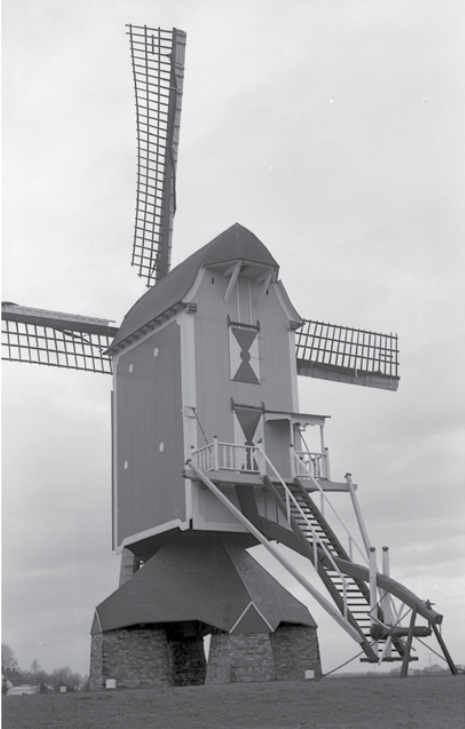
\includegraphics[width=0.75\textwidth]{ch1_introduction/images/postwindmill.png}
        \caption{A post wind mill in the Netherlands.}
    \end{subfigure}
    ~ %add desired spacing between images, e. g. ~, \quad, \qquad, \hfill etc. 
      %(or a blank line to force the subfigure onto a new line)
    \begin{subfigure}[b]{0.45\textwidth}
    \captionsetup{justification=centering}
        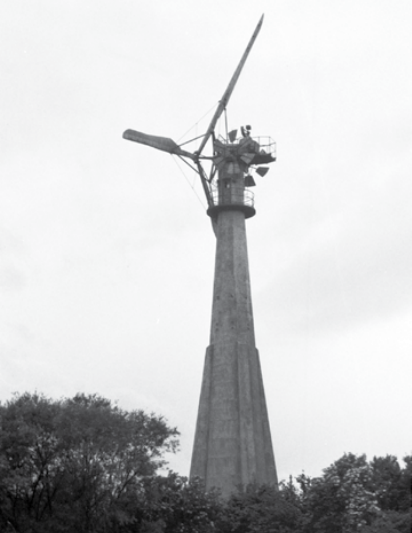
\includegraphics[trim=0 0 0 0,clip,width=0.9\textwidth]{ch1_introduction/images/Smidth-Aeromotor_fig120hist.png}
        \caption{Smidth-Aeromotor in Denmark.}
    \end{subfigure}
    \caption{Wind mills used for mechanical drives (a) and an out of service Smidth-Aeromotor in Denmark with a nominal output of $70kW$ (b)~\cite{beurskens2014history}.}
    \label{fig:windturbex1}
\end{figure}
\begin{figure}[h!]
    \centering
    \captionsetup{justification=centering}
 \begin{subfigure}[b]{0.45\textwidth}
 \centering
    \captionsetup{justification=centering}
        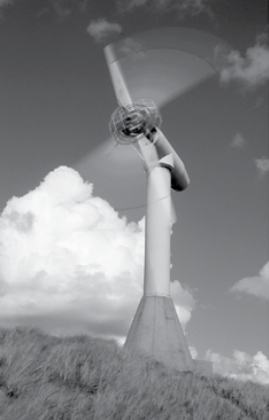
\includegraphics[trim=0 0 0 0,clip,width=0.45\textwidth]{ch1_introduction/images/petten_25mhawt.png}
        \caption{The $25 m$ HAT wind turbine in operation at Petten ($0.4 MW$ rated capacity)~\cite{beurskens2014history}.}
    \end{subfigure}
    \begin{subfigure}[b]{0.45\textwidth}
    \centering
    \captionsetup{justification=centering}
        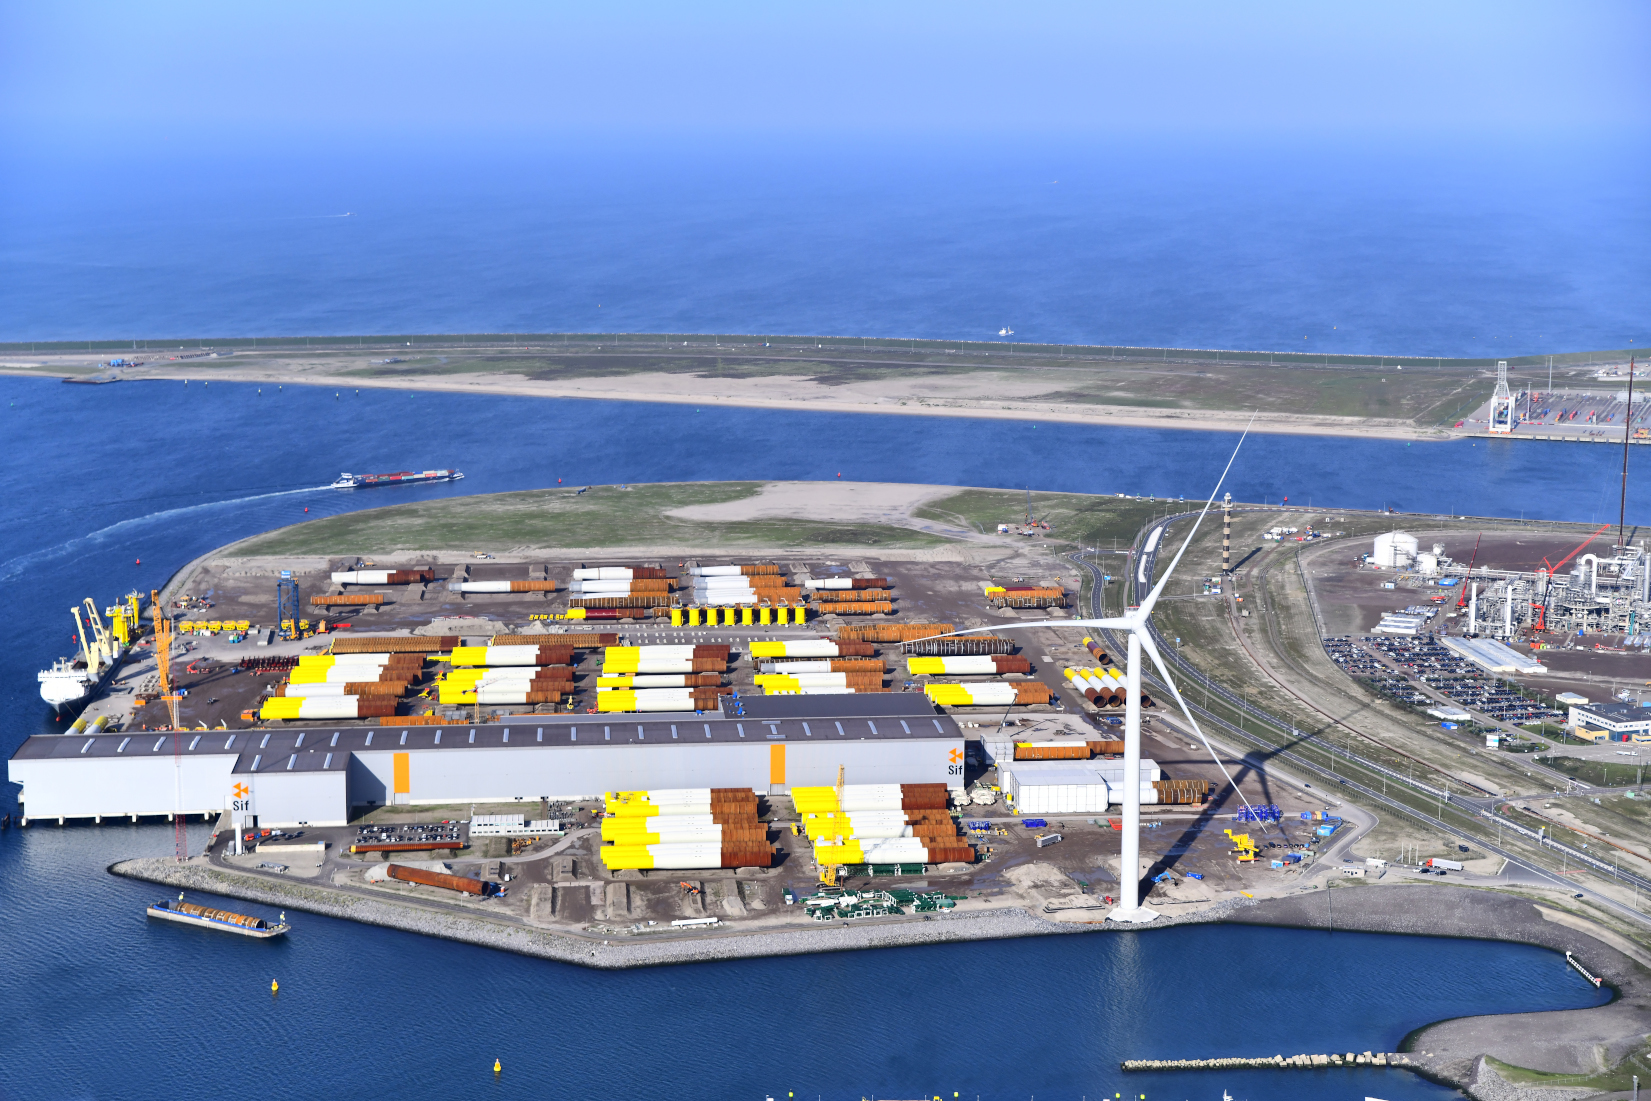
\includegraphics[width=0.9\textwidth]{ch1_introduction/images/gehaliadex.jpg}
        \caption{The $12 MW$ GE Haliade X at the port of Rotterdam~\cite{GE}.}
    \end{subfigure}
    \caption{Evolution of wind turbines, from producing $<1 MW$ in 1980s (a) to large wind turbines producing $>10 MW$ today (b).}
    \label{fig:windturbex2}
\end{figure}

\section{Wind energy in the current energy climate}
While a period of steady but unspectacular growth in wind energy was observed in the early 1990s, in recent times it has grown spectacularly (figure~\ref{fig:wind_inst_hist}). Wind energy is expected to play a crucial role in transitioning towards a zero carbon energy sector. 
\begin{figure}[h!]
\centering
\captionsetup{justification=centering}
 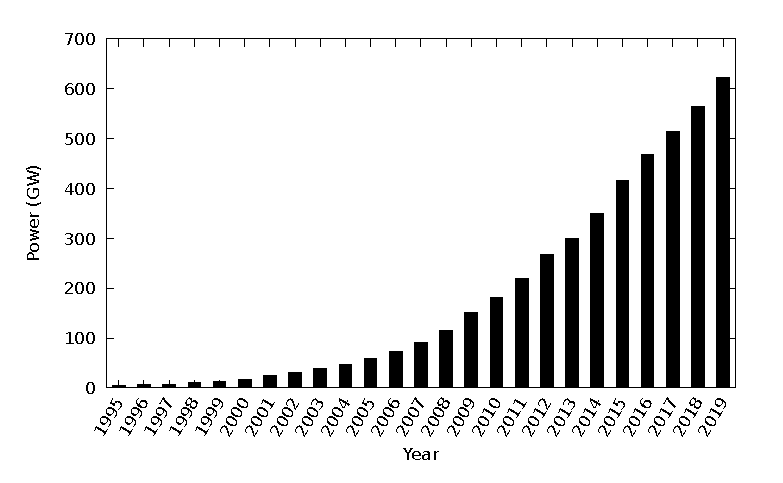
\includegraphics[width=0.85\textwidth]{ch1_introduction/images/wind_inst_cap_hist.eps}
\caption{Worldwide cumulative installed capacity of wind energy over time.}
 \label{fig:wind_inst_hist}
\end{figure} 
Constant improvements in wind turbine design has led to larger and larger wind turbines (figure~\ref{fig:wind_rotor}). Larger wind turbines (see figure~\ref{fig:windturbex2}) have driven installation costs per megawatt (MW) down which is reflected in the massive cost reduction for both onshore and offshore wind turbines. The global weighted-average levelized cost of energy (LCOE) of projects  using this technology and commissioned in 2019 was USD 0.053/kWh — $9\%$ lower than in 2018 and $39\%$ lower than in 2010, when it was USD 0.086/kWh. Onshore wind energy now consistently outcompetes even the cheapest fossil fuel fired source of electricity, while costs continue to decrease~\cite{irenareport}. 
\begin{figure}[h!]
\centering
\captionsetup{justification=centering}
 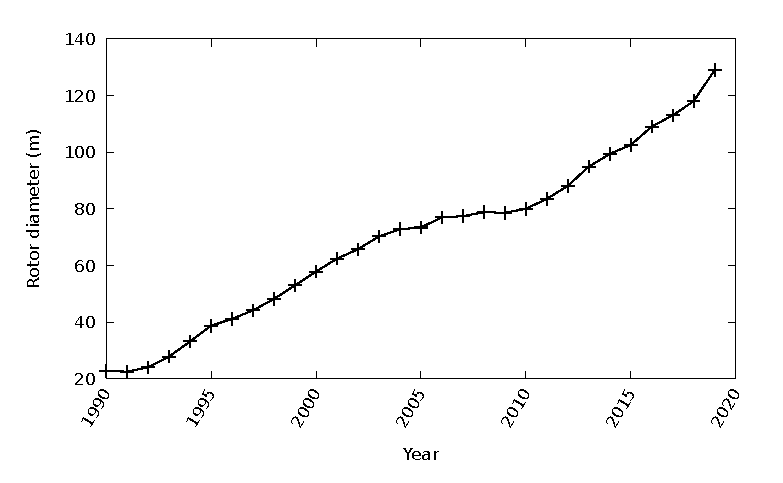
\includegraphics[width=0.85\textwidth]{ch1_introduction/images/wind_rotor_size.eps}
\caption{Rotor diameter size over years~\cite{rotorsize}.}
 \label{fig:wind_rotor}
\end{figure} 

Research on wind turbine aerodynamics have played a huge role in improving the performance of turbine blades over the years. Aerodynamicists have a variety of tools at their disposal. Over the years field experiments, wind tunnel measurements and computational tools have all been used to push the envelope of wind turbine aerodynamics. Looking ahead, the wind turbines are likely to become increasingly efficient and complex. To facilitate tackling the upcoming challenges, the tools used for research must also improve. Uncertainties in research tools must be reduced by using higher fidelity tools to keep up with the growth of technology. 

\section{Wind turbine aerodynamics}

Wind turbines operate at high Reynolds numbers and low Mach numbers which is somewhat unique compared to other external aerodynamic applications like aerospace, and greatly advantageous in terms of numerical analysis. The high Reynolds number means large regions of the flow can be considered inviscid except for a small region around the body known as the boundary layer (figure~\ref{fig:zonal}). The low Mach numbers imply that the flow remains incompressible. This combination of conditions have been exploited to develop a wide variety of numerical tools based on simplified forms of the Navier-Stokes equations.
\begin{figure}[h!]
\centering
\captionsetup{justification=centering}
 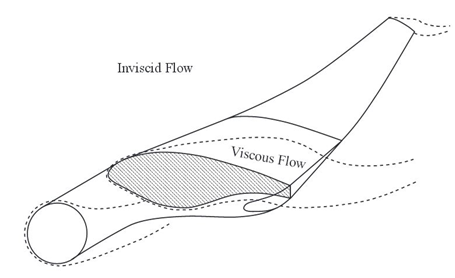
\includegraphics[width=0.5\textwidth]{ch1_introduction/images/zonal.png}
\caption{Inviscid flow and boundary layer regions~\cite{katz_plotkin_2001} for the flow around a wind turbine blade.}
 \label{fig:zonal}
\end{figure} 
On the other hand, aerodynamic analysis of wind turbines remains very challenging because of the disparate range of the scales involved (figure~\ref{fig:scales}). The relevant length scales range from boundary layers on the turbine blades that  are a few millimeters thick all the way upto wind farms that are tens of kilometers long. 
\begin{figure}[h!]
\centering
\captionsetup{justification=centering}
 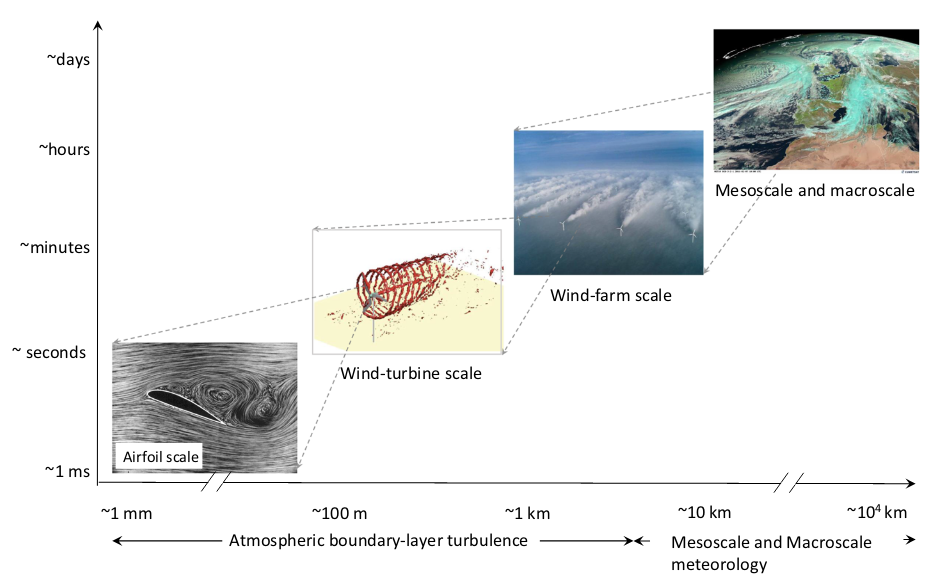
\includegraphics[width=0.75\textwidth]{ch1_introduction/images/scales_porteagel.png}
\caption{Range of scales of flow that are relevant in wind turbine aerodynamics~\cite{porte2020wind}.}
 \label{fig:scales}
\end{figure} 

In the following sections, a review of wind turbine aerodynamics is presented in three parts - aerodynamics of airfoils, aerodynamics of rotors and wind farm analysis.

\subsection{Airfoil analysis}\label{ssec:ch1airfoil}
Airfoil aerodynamics is at the heart of wind turbine rotor aerodynamics. Two dimensional analysis of airfoils is required by many different rotor design methods. Also analyzing the flow over a simpler two dimensional airfoil can give much needed insight into the physics of wind turbine aerodynamics under complex flow conditions. Due to wind turbines operating at very high Reynolds numbers, the flow around airfoils can be divided into the boundary layer very near the airfoil surface and an inviscid region away from the surface. While the boundary layer region is crucial in many applications, the inviscid analysis can also give useful information especially in attached flow regions. By neglecting the effect of viscosity and assuming the flow to be irrotational, potential flow analysis can be used. Panel methods~\cite{katz_plotkin_2001} are very popular for the inviscid analysis of airfoils. The boundary layer can be analyzed separately by solving the simplified boundary layer equations~\cite{Lyon2014}. Integral boundary layer methods can further simplify the two dimensional boundary layer equations into a one dimensional problem. Combination of the boundary layer methods with potential flow methods can give the global flow field. This is known as the interacting boundary layer approach~\cite{Ozdemir2020} which is used in tools like XFOIL~\cite{drela1989xfoil} and RFOIL~\cite{rfoil_orig}.

However, the simplified analysis methods are only valid under attached flow conditions. While inviscid flow methods cannot be used to analyze separated flow, even boundary layer methods loose accuracy under such conditions. Passive flow control devices like vortex generators are widely used to improve the performance of the airfoil and delay separation. Potential flow methods and boundary layer methods cannot be used for such complex geometries readily. With increasing use of wind turbines in adverse weather conditions, rotor blades are also subject to erosion. Modeling such effects are also not yet possible with lower fidelity tools. 
\begin{figure}[h!]
\centering
\captionsetup{justification=centering}
 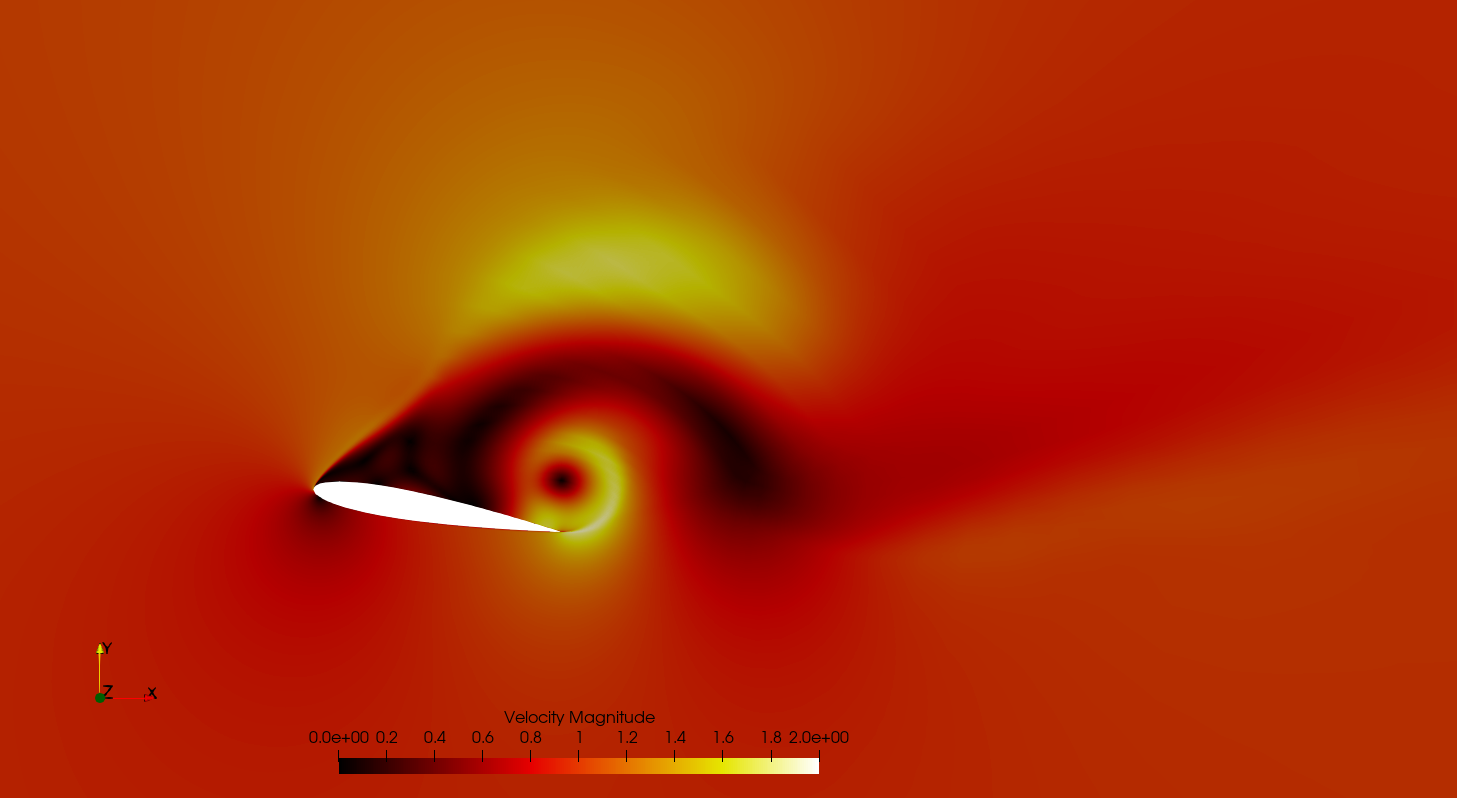
\includegraphics[width=0.5\textwidth]{ch1_introduction/images/airfoil_picture.png}
\caption{Velocity contours for a flow past an airfoil.}
 \label{fig:airfoil}
\end{figure} 

Computational Fluid Dynamics (CFD) methods do not have such limitations as the incompressible Navier Stokes equations are solved without any of the simplifying assumptions used for the methods mentioned above. Reynolds Averaged Navier Stokes (RANS) based methods are more widely used in combination with turbulence modeling, but the use of Large Eddy Simulations (LES), and hybrid LES methods are gaining traction. Some of the challenges for CFD in airfoil aerodynamics are the prediction of laminar to turbulent transition and flow separation.



\subsection{Rotor modeling}
%Blade aerodynamics - BEM, lifting line, Panel methods, CFD RANS, CFD DES (LES) ..
The design of rotor blades is a multi-disciplinary endeavour including aerodynamic analysis and structural design. Focusing on the aerodynamics only, due to faster computational times the Blade Element Momentum (BEM) theory is widely used in the early stages of the design process. The rotor design from BEM is then evaluated by an aeroelastic tool and if the design turns out to be efficient, it is evaluated by more advanced and accurate methods~\cite{bak2011aerodynamic} like CFD. The rotor design is carried out with the intention of maximizing Annual Enegy Production (AEP) which is traditionally done by a mixture of designer experience and numerical optimization. Due to this iterative nature of the design process, computational speed at a reasonable accuracy overrides other criteria for selecting numerical tools. 

BEM theory is the oldest method~\cite{windenergyexp, bak2011aerodynamic} that has been constantly improved over the years~\cite{Gerardthesis}. The local blade element theory is used in combination with the one dimensional momentum theory. The assumptions are that the flow is inviscid and there are no losses. The rotor plane is assumed to be an ideal and permeable disc that extracts energy~\cite{windenergyexp, bak2011aerodynamic}. Design of rotor blades is done iteratively based on two dimensional airfoil characteristics which can be found using the methods described in section~\ref{ssec:ch1airfoil} .

Vortex wake methods are a more accurate representation of the flow field around rotors. The flow is still assumed to be steady, but the rotor geometry is represented either as a lifting line~\cite{awsm_arne} or a lifting surface~\cite{katz_plotkin_2001}. Trailing and shed vortices are computed based on local flow conditions and airfoil characteristics. These vortices are then convected into the wake. In a lifting line model, the blade is represented by a single line with bound vorticity that varies radially. For lifting surfaces, the blade is represented by a zero thickness surface along the camber line instead of assuming that all lift is concentrated along a line, as is done in the lifting line theory. Three dimensional panel methods represent the exact geometry of the blade and are also used for rotor analysis. Similar to the two dimensional scenario, a potential flow solution is sought~\cite{katz_plotkin_2001, arne_phd}.
All the methods described so far are inviscid and as the fidelity of the representation of rotor increases from the lifting line to lifting surface and finally to the panel method, so does the computational requirements. 

CFD has also been used for rotor blade analysis. The first RANS simulations on wind turbine rotors were performed in the late 1990s and early 2000s~\cite{duque2000numerical, sorensen1998rotor, varela1999cfd}. A detailed historical overview of the use of CFD in rotor modeling can be found in Sumner et al~\cite{sumner2010cfd}. While the use of RANS turbulence models is still common, there have been some hybrid LES studies on rotors reported recently~\cite{criticalreview}. 

The inviscid methods rely to some extent on two dimensional airfoil characteristics and are prone to missing some three dimensional phenomena like rotational augmentation where it is observed that the inboard sections of blades produce lift and drag that is significantly different from the two dimensional characteristics~\cite{sumner2010cfd, schreck2002rotational}. Performing full three dimensional CFD analysis of rotors overcomes this limitation but that comes with an increase in computational cost. Some authors~\cite{xu2002development, schmitz2005parallelized} have proposed the use of a hybrid between CFD and inviscid vortex based methods. The region close to the rotor is modeled using CFD and the flow outside is modeled as inviscid using the inviscid methods described earlier. Hybrid approaches are especially useful in studying wake aerodynamics. 
\begin{figure}[h!]
\centering
\captionsetup{justification=centering}
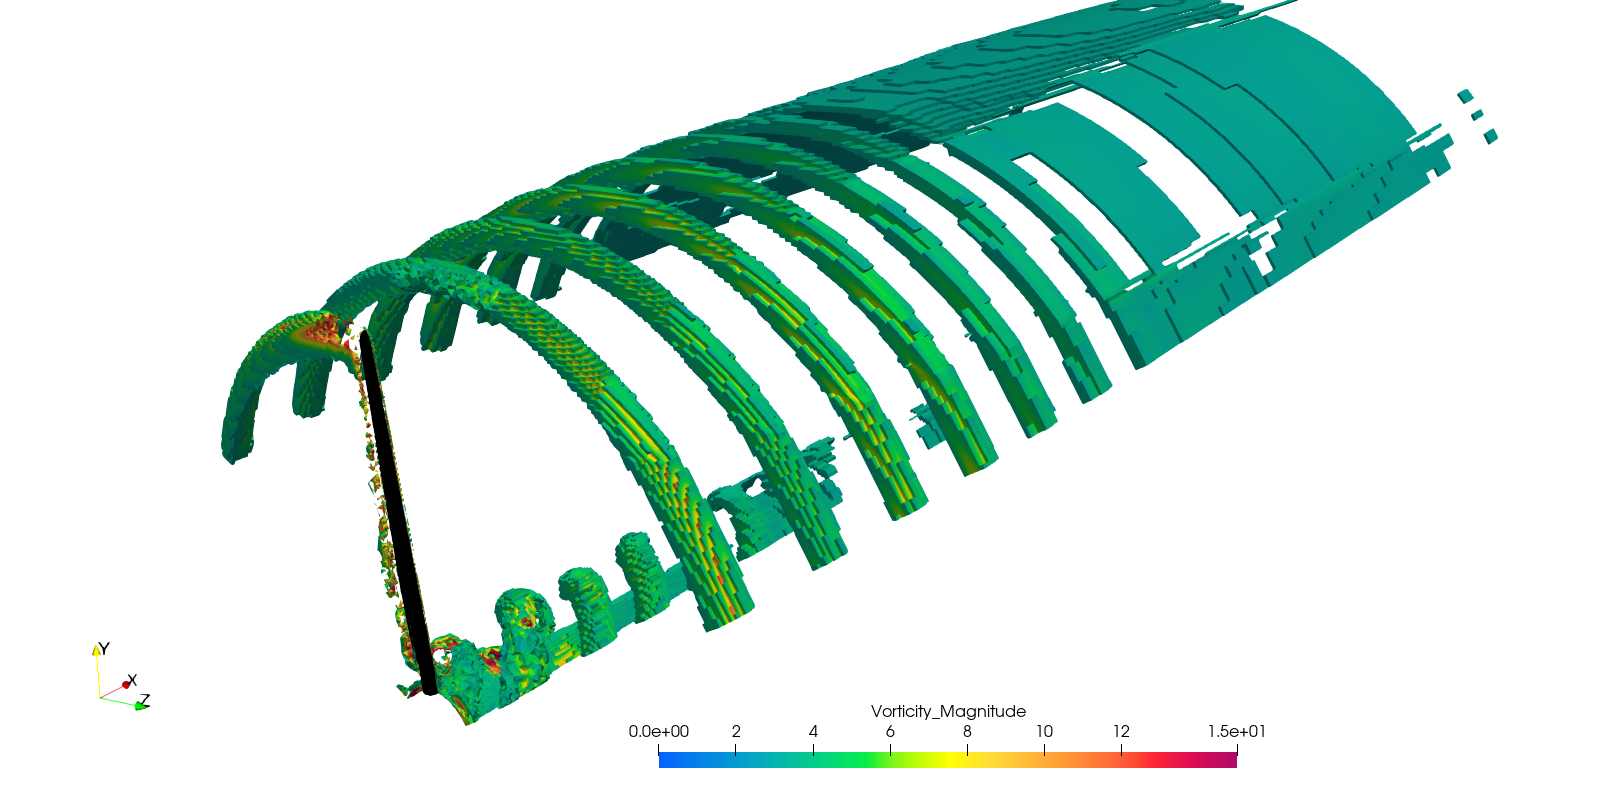
\includegraphics[width=\textwidth]{ch1_introduction/images/turbine_wake_picture2.png}
\caption{Vortex structures behind a turbine blade (periodic CFD simulation).}
 \label{fig:rotor}
\end{figure} 

Another alternative to modeling rotor blades in CFD is the use of an actuator disc (AD)~\cite{aagaard1982actuator, rajagopalan1985finite}. The AD method is based on the blade element theory and represents the rotor with an equivalent porous surface and it is modeled as a source term that acts on the flow in that region. However, this method is mostly used to model wind farms to study the behavior of wakes which is the subject of the next section.

\subsection{Wind farms} 
The wakes emanating from wind turbines are unsteady and highly turbulent. In addition, these wakes also interact with the atmospheric boundary layer which is also dynamic and turbulent. Also wind turbines, especially offshore turbines, are clustered in large wind farms to reduce installation and maintenance costs. Because of the relatively close spacing however, the wake from the turbines interact with each other in addition to the atmospheric boundary layer. Turbines that are downstream of another turbine can see power losses in the range of $40\%$ in full wake conditions and experience increased fatigue loads~\cite{porte2020wind, stevensreview, sandresereview}.

The wind turbine wake can be divided into two regions~\cite{vermeer2003wind} - the near wake region that extends about $2$-$4$ rotor diameters downstream from the turbine and the far wake which is further downstream (see figure~\ref{fig:ablwake}). The near wake region is influenced greatly by wind turbine features like blade profile, nacelle and is highly complex and three dimensional. The far wake region, however, is influenced more by wind turbine parameters such as thrust and power coefficients, incoming flow etc. As the spacing between any two turbines in a wind farm is larger than the near wake, modeling the far wake accurately is more important than the near wake for understanding wind farm aerodynamics.
\begin{figure}[h!]
\centering
\captionsetup{justification=centering}
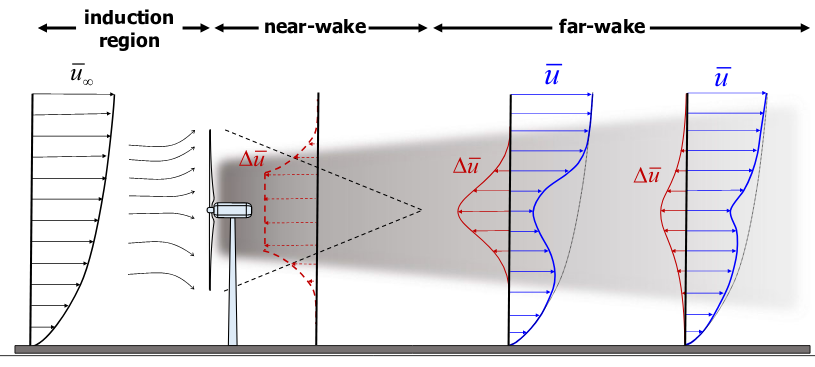
\includegraphics[width=0.75\textwidth]{ch1_introduction/images/wake_regions.png}
\caption{Schematic figure from Port{\'e}-Agel et al.~\cite{porte2020wind} showing the time averaged flow features resulting from the interaction of a wind turbine with the incoming turbulent (atmospheric) boundary layer.}
 \label{fig:ablwake}
\end{figure} 


Numerical modeling of wakes is done either using analytical models or the use of three dimensional CFD analysis where the rotors are represented as an actuator disc or line or surface~\cite{sorensonal, sandresereview}. Analytical models are used to predict the velocity deficit caused by the wind turbine wakes. These models have a lower accuracy compared to full 3D CFD simulations but have a very low computational cost. Analytical models mostly aim to predict the mean velocity deficit and do not consider the turbulence properties in the wake that can be significantly different from the undisturbed flow field. Thus, they are commonly used for design purposes like optimization of the wind farm layout, control of wind farms and other multi-disciplinary simulations. RANS modeling of wind farms have been extensively studied. Steady state tools like RANS are not suitable for capturing important dynamic wake effects that can significantly affect wind turbine loading.
As computational resources have improved, the use of LES to study wind farm aerodynamics have become very common~\cite{stevensreview, criticalreview}.

Reviews of wind turbine wake aerodynamics can be found in literature (for example, Sanderse et al~\cite{sandresereview},  Port{\'e}-Agel et al.~\cite{porte2020wind}, Stevens and Meneveau~\cite{stevensreview}, Th{\'e} and Yu~\cite{criticalreview}).



%\section{Outlook}
%However as the size of the turbine blades has increased, issues like thick airfoils, transition modeling are becoming more important. Additionally, new concepts to improve the efficiency of the turbines (e.g. vortex generators) are becoming more common. While it is possible to extend the existing tools like RFOIL to account for some of the new problems\cite{Ramanujam2016, Ramanujam2017, doublewake} arising out of modern wind turbine blades, they are still limited in their scope of applicability. Thus, a higher fidelity general purpose tool like CFD becomes necessary.
\subsection*{Looking ahead}
From the preceding section it can be seen that despite the vast range of scales involved in wind turbine aerodynamics, CFD methods are regularly used in all cases. As wind turbines become more complex, the use of a higher fidelity tool like CFD will become more prevalent. Additionally, CFD tools are increasingly being used in multi disciplinary problems like fluid structure interaction~\cite{hsu2012fsi, wang2016fsi, airfoilfsi}, shape optimization~\cite{madsenshapeopt, dhertshapeopt}, uncertainty quantification~\cite{andresuq, hsiehuq}, aeroacoustics~\cite{luolesacoust, edisonacoust} to name a few. It must be noted that the references cited here are only a small selection of the state of the art. While industrial adoption of CFD for the full rotor design is likely far away in the future, CFD methods are increasingly being used earlier in the design process instead of just being used for evaluation purposes. 

\section{Goal}

The main aim of this thesis is to develop a new pressure based solver within the framework of the open source multi-physics suite SU2~\cite{SU22013}. The immediate goals are to use this solver for various wind turbine aerodynamics applications like rotor simulations, vortex generator modeling and improving lower fidelity tools. In the long term, the goal is to take advantage of the open source nature of SU2 to not only improve the solver for aerodynamic applications but also to use it as a base for multi disciplinary applications like fluid structure interaction, aeroacoustics and optimization. 

\section{Dissertation overview}
This thesis can be broadly divided into two parts - Chapters 2, 3 and 4 are devoted to the implementation details of the new pressure based solver in SU2 while chapters 5, 6 and 7 focus on different applications of CFD in wind energy. 

Chapter 2 describes the governing equations for incompressible flow and different methods to solve them. First a short overview of the incompressible Navier Stokes equations is presented. The finite volume method that is commonly used in CFD is described for a general scalar equation highlighting the various numerical aspects. Subsequently, the challenges when dealing with the incompressible flow equations and different methods to overcome them are described. Finally, an overview on turbulence modeling for incompressible flows is given.

Chapter 3 describes the implementation of the governing equations and solution methods outlined in chapter 2 into SU2. 

Chapter 4 presents some verification and validation results for the new solver. Verification of the accuracy of the solver is carried out against analytical solutions. Different test cases that replicate different conditions faced in wind turbine aerodynamics are chosen to validate the solver. 

Chapter 5 presents the first steps towards modeling vortex generators in integral boundary layer methods. First a conceptual overview of the effect of vortex generators (VGs) on turbulent boundary layers is presented. CFD simulations of VGs on flat plates is then used to introduce the modeling approach. 
%Finally, a preliminary VG model is applied to a flat plate integral boundary layer tool and the results are compared against CFD results.

Chapter 6 presents the effect of leading edge erosion using roughness models for eddy viscosity based RANS turbulence models. The performance of the roughness models is first validated against empirical formulations and experimental data for a flat plate and airfoils. Different methods to characterize roughness numerically are surveyed. Finally, the impact of roughness on turbulent boundary layers are studied and future research required to model roughness in integral boundary layers are presented. 

Chapter 7 will present preliminary results from the CFD analysis of the widely studied New Mexico rotor blade.

\bibliographystyle{dissertation}
\bibliography{ch1_introduction/ch1bib}


%\begin{figure}[h!]
%\centering
%\captionsetup{justification=centering}
% 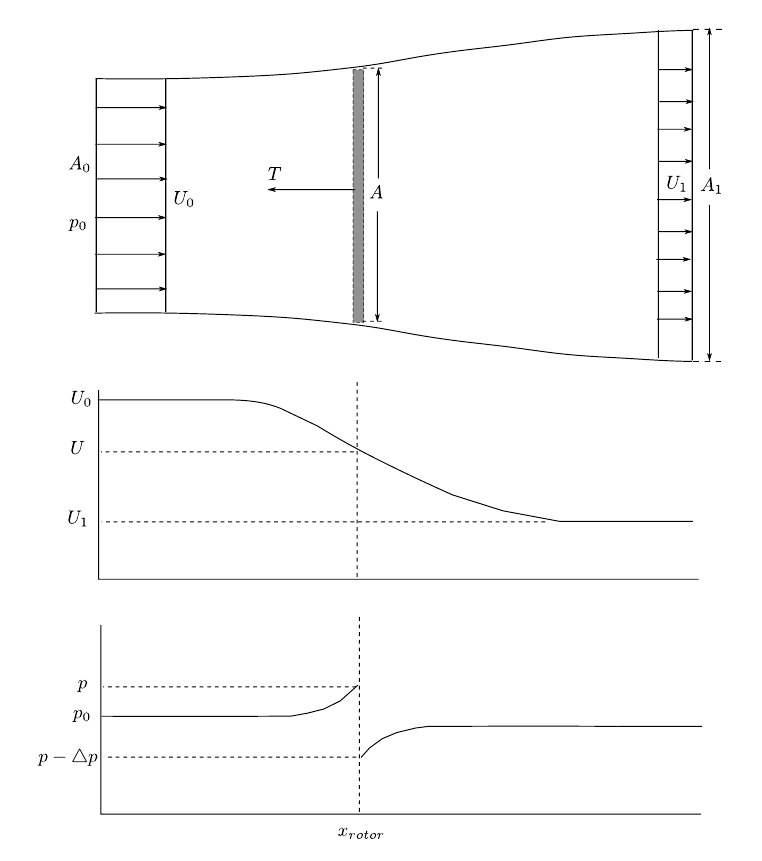
\includegraphics[width=0.65\textwidth]{ch1_introduction/images/BEM_rotor_plane.png}
%\caption{Flow through the wind turbine rotor plane for BEM analysis~\cite{zhangthesis}.}
% \label{fig:bemintro}
%\end{figure} 

%\begin{figure}[h]
%    \centering
%    \begin{subfigure}[b]{0.45\textwidth}
%    \centering
%    \captionsetup{justification=centering}
%        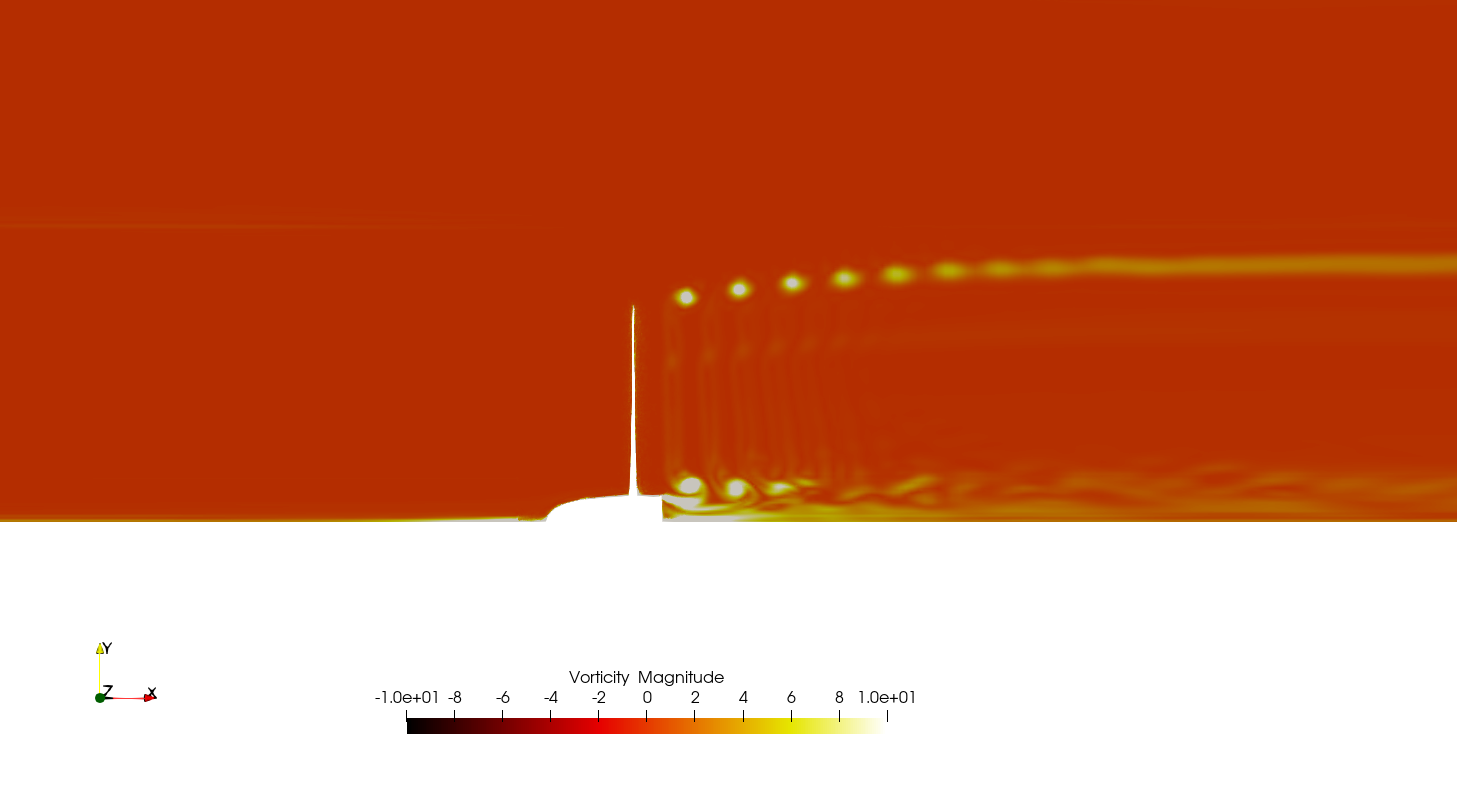
\includegraphics[width=.75\textwidth]{ch1_introduction/images/turbine_picture.png}
%        \caption{Vorticity contour for flow past a turbine blade.}
%    \end{subfigure}
    ~ %add desired spacing between images, e. g. ~, \quad, \qquad, \hfill etc. 
      %(or a blank line to force the subfigure onto a new line)
%    \begin{subfigure}[b]{0.45\textwidth}
%    \centering
%    \captionsetup{justification=centering}
%        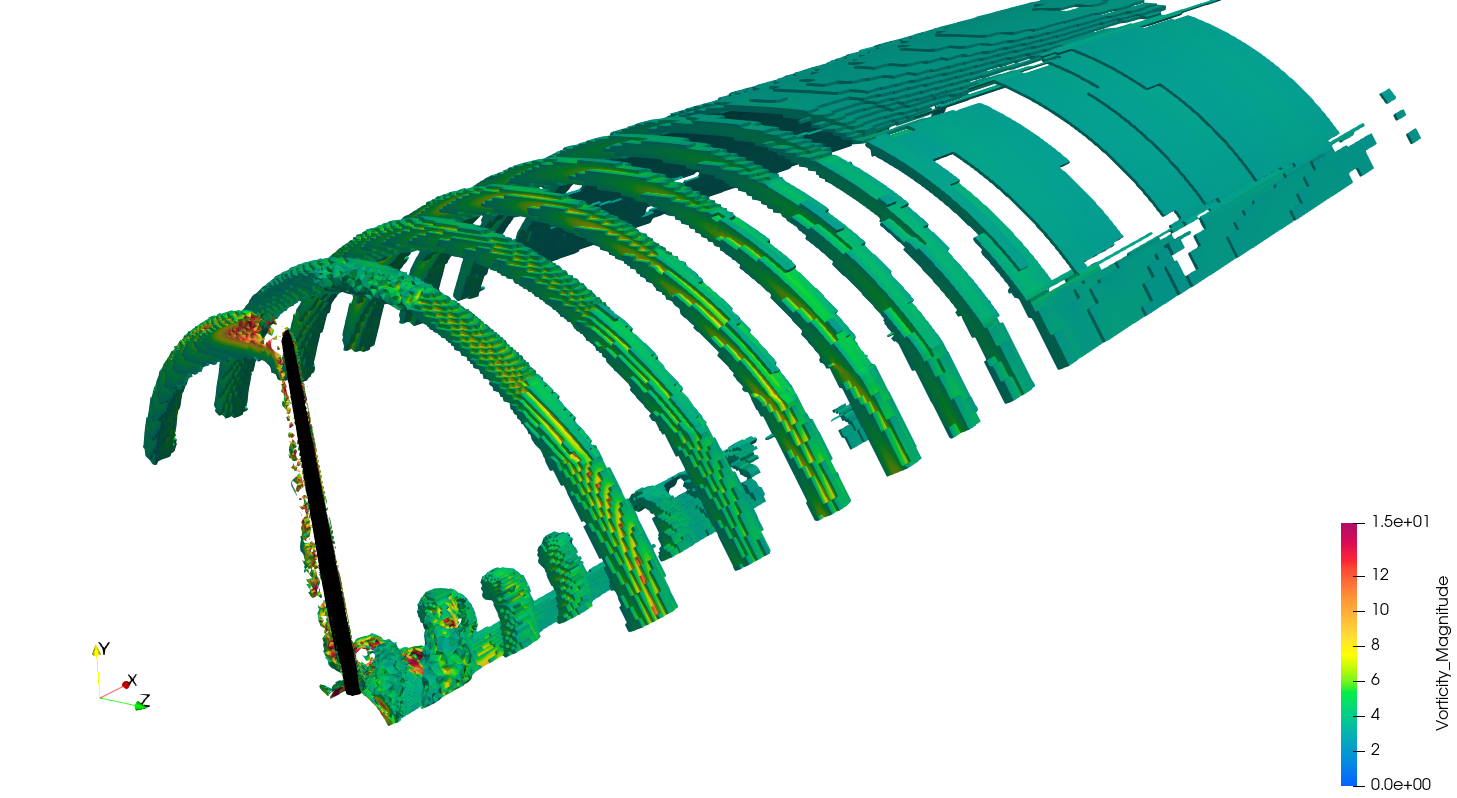
\includegraphics[width=0.75\textwidth]{ch1_introduction/images/turbine_wake_picture.png}
%        \caption{Vorticity shed from the turbine blade (periodic simulation).}
%    \end{subfigure}
%    \label{fig:rotor}
%    \caption{Vorticity contour for flow past a turbine blade.}
%\end{figure}

\chapter[Incompressible flow equations]{Incompressible flow equations}
\label{ch:ch2incompeq}

%% The following annotation is customary for chapter which have already been
%% published as a paper.
%\blfootnote{This chapter has been submitted to the Journal of Fluid Mechanics.}
%\blfootnote{footnote}
\begin{abstract}
In this chapter the governing equations and solution methods for incompressible flows are presented. The incompressible Navier Stokes equations are first given in dimensional and non-dimensional forms. Subsequently, the finite volume method applied to a general conservation equation is described. The difficulty associated with solving the incompressible flow equations numerically, namely the pressure velocity coupling, is described and the different methods to overcome this issue are presented. Finally, the solution procedure to solve turbulent incompressible flow equations are shown.
\end{abstract}
%This chapter presents the governing equations for incompressible flow and describes  different solution methods. 
\section{Navier Stokes equations}
The governing flow equations for incompressible flow with constant density and viscosity and no heat transfer are 
\begin{equation}
\frac{\partial (\rho u)}{\partial x} + \frac{\partial (\rho v)}{\partial y} + \frac{\partial (\rho w)}{\partial z} = 0,
\label{eq:continuity}
\end{equation}
\begin{equation}
\frac{\partial (\rho u)}{\partial t} + \frac{\partial (\rho u u)}{\partial x}+ \frac{\partial (\rho uv)}{\partial y} + \frac{\partial (\rho uw)}{\partial z} = -\frac{\partial p}{\partial x} + \mu\left(\frac{\partial^2 u}{\partial x^2} + \frac{\partial^2 u}{\partial y} + \frac{\partial^2 u}{\partial z}\right)
\label{eq:xmommentum}
\end{equation}
\begin{equation}
\frac{\partial (\rho v)}{\partial t} + \frac{\partial (\rho uv)}{\partial x}+ \frac{\partial (\rho vv)}{\partial y} + \frac{\partial (\rho vw)}{\partial z} = -\frac{\partial p}{\partial y} + \mu\left(\frac{\partial^2 v}{\partial x^2} + \frac{\partial^2 v}{\partial y} + \frac{\partial^2 v}{\partial z}\right)
\label{eq:ymommentum}
\end{equation}
\begin{equation}
\frac{\partial (\rho w)}{\partial t} + \frac{\partial (\rho wu)}{\partial x}+ \frac{\partial (\rho wv)}{\partial y} + \frac{\partial (\rho ww)}{\partial z} = -\frac{\partial p}{\partial z} + \mu\left(\frac{\partial^2 w}{\partial x^2} + \frac{\partial^2 w}{\partial y} + \frac{\partial^2 w}{\partial z}\right)
\label{eq:zmommentum}
\end{equation}
where $\rho$ is the constant density of the fluid, $u$, $v$ and $w$ are the $x-$, $y-$ and $z-$ components of the velocity vector respectively, $p$ is the pressure and $\mu$ is the dynamic viscosity, assumed to be constant. Equation~\ref{eq:continuity} is the continuity equation or the mass conservation equation. For incompressible flows, this condition reduces to a zero divergence condition for the velocity vector. Equations~\ref{eq:xmommentum}, \ref{eq:ymommentum} and \ref{eq:zmommentum} are the momentum conservation equations in $x$, $y$ and $z$ directions respectively. Here it is assumed that the fluid is Newtonian. Under the incompressible flow assumption the energy equation is decoupled from the continuity and momentum equations and is therefore not shown here.
\subsection{Non-dimensionalization}
All the quantities in equations~\ref{eq:continuity}, \ref{eq:xmommentum}, \ref{eq:ymommentum} and \ref{eq:zmommentum} are dimensional and their magnitudes can vary widely. The governing equations can be transformed into a non dimensional form by scaling the variables using reference values. The scaling parameters can be defined as follows
\begin{list}{}{}
	\item $L$ - reference length (e.g. chord of the airfoil),
	\item $V$ - reference velocity (e.g. the free stream velocity, $V_{\infty}$),
	\item $f$ - characteristic frequency (e.g., one cycle of a periodic process, or $V/L$),
	\item $p_0$ - reference pressure (e.g., dynamic pressure, $\rho V_{\infty}^2$).
\end{list}

With the aid of these characteristic quantities we can define the following non-dimensional variables
\begin{equation*}
	x^*=\frac{x}{L}, \quad y^*=\frac{y}{L}, \quad z^*=\frac{z}{L},
\end{equation*}
\begin{equation*}
	u^*=\frac{u}{V}, \quad v^*=\frac{v}{V}, \quad w^*=\frac{w}{V},
\end{equation*}
\begin{equation*}
	p^*=\frac{p}{p_0}=\frac{p}{\rho V^2}, \quad t^*= tf.
\end{equation*}
Based on dimensional analysis, the following non dimensional numbers can be defined
\begin{equation}
St = \frac{fL}{V}, \label{eq:Stdefn} 
\end{equation}
\begin{equation}
Re = \frac{V L}{\nu} , \label{eq:Redefn}
\end{equation}
where $St$ is known as the Strouhal number and $Re$ is the Reynolds number. $\nu=\frac{\mu}{\rho}$ is the kinematic viscosity. Using the non-dimensional variables and the new non dimensional numbers, equation~\ref{eq:continuity} can be written as:
\begin{equation*}
\frac{\partial u^*}{\partial x^*} + \frac{\partial v^*}{\partial y^*} + \frac{\partial w^*}{\partial z^*}= 0,
\end{equation*}
and the equations~\ref{eq:xmommentum}, \ref{eq:ymommentum} and \ref{eq:zmommentum} as 
\begin{equation*}
St \frac{\partial u^*}{\partial t^*} + \frac{\partial (u^* u^*)}{\partial x^*} +  \frac{\partial (u^* v^*)}{\partial y^*} + \frac{\partial (u^* w^*)}{\partial z^*} = -\frac{p_0}{\rho V^2}\frac{\partial p^*}{\partial x*} + \frac{1}{Re}\left( \frac{\partial^2 u^*}{\partial x^{*2}} + \frac{\partial^2 u^*}{\partial y^{*2}} + \frac{\partial^2 u^*}{\partial z^{*2}}\right),
\end{equation*}
\begin{equation*}
St\frac{\partial v^*}{\partial t^*} + \frac{\partial (v^*u^*)}{\partial x^*} + \frac{\partial (v^*v^*)}{\partial y^*} +\frac{\partial (v^*w^*)}{\partial z^*} = -\frac{p_0}{\rho V^2}\frac{\partial p^*}{\partial y*} + \frac{1}{Re}\left( \frac{\partial^2 v^*}{\partial x^{*2}} + \frac{\partial^2 v^*}{\partial y^{*2}} + \frac{\partial^2 v^*}{\partial z^{*2}}\right),
\end{equation*}
\begin{equation*}
St\frac{\partial w^*}{\partial t^*} + \frac{\partial (w^*u^*)}{\partial x^*} + \frac{\partial (w^*v^*)}{\partial y^*} +\frac{\partial (w^*w^*)}{\partial z^*} = -\frac{p_0}{\rho V^2}\frac{\partial p^*}{\partial z*} + \frac{1}{Re}\left( \frac{\partial^2 v^*}{\partial x^{*2}} + \frac{\partial^2 v^*}{\partial y^{*2}} + \frac{\partial^2 v^*}{\partial z^{*2}}\right).
\end{equation*}
If the reference values are chosen judiciously, the comparison of the different non dimensional quantities can yield information about the relative importance of different flow features. Additionally, matching the non dimensional parameters will allow for comparison of data across different experiments and numerical simulations. 

The above equations can be written more compactly using the index notation (see below). In addition to using the index notation, the time and pressure references are chosen as $f = V/L$ and $p_0 = \rho V^2$ leading to the coefficients of the unsteady term and the pressure gradient term to be unity. The $\ast$ is dropped for the sake of convenience but all quantities shown are non dimensional.
\begin{equation}
\frac{\partial u_i}{\partial x_i} = 0,
\label{eq:contindx}
\end{equation}
\begin{equation}
\frac{\partial u_i}{\partial t} + \frac{\partial (u_iu_j)}{\partial x_j} = -\frac{\partial p}{\partial x_i} + \frac{1}{Re}\left( \frac{\partial^2 u_i}{\partial x_j\partial x_j} \right).
\label{eq:momindx}
\end{equation}
Here the velocities are represented by $u_i$, with $i=1,2,3$ being the three components of the velocity vector and similarly $x_i$ represents the three coordinate directions. Repeated indices indicate a summation over that index. Thus, equation~\ref{eq:momindx} represents the three momentum equations.

The rest of the thesis will use index notation to keep the equations compact.

\section{Numerical methods}
%Describe numerical methods - briefly introduce FVM and show discretization.
The equations described in the previous section cannot be solved analytically except for some simplified cases and are solved numerically. Consider the example of a typical flow problem - the flow past a cylinder. The region of interest extends outwards from the cylinder as shown in figure~\ref{fig:airfoildom}. 
\begin{figure}[h!]
\centering
\captionsetup{justification=centering}
 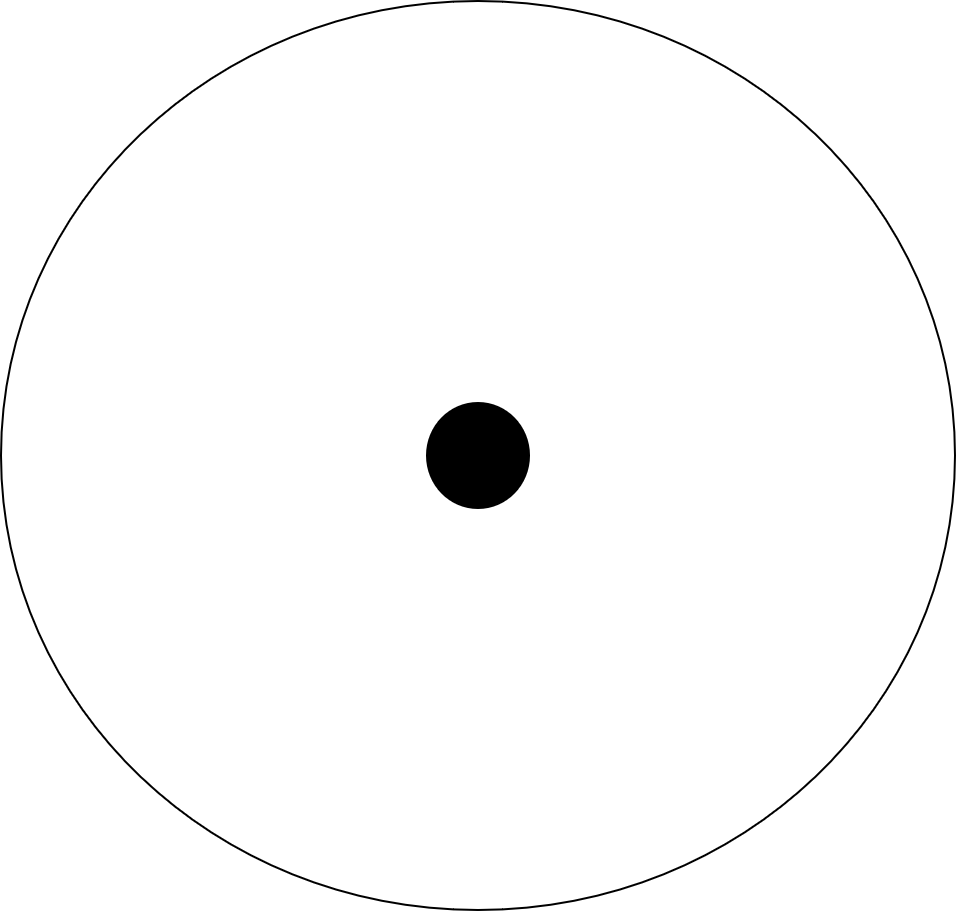
\includegraphics[width=0.55\textwidth]{ch2_litsurvey/Figures/airfoil_domain.png}
\caption{Region of interest for flow over a cylinder.}
 \label{fig:airfoildom}
\end{figure} 
In order to find the velocities and pressures in this region, the physical domain is divided into smaller domains where the partial differential equations can be approximated in a simpler manner. This process is known as \textit{discretization}. Since the partial differential equations are non-linear, care must be taken during the discretization process to preserve all the important flow phenomena in the approximate equations as well. 

However, in order to solve the approximate equations numerically, they must converted into algebraic equations. The equations are then solved at some specified points (\textit{nodes} or \textit{grid points}) within each of the smaller domains. This process can be done using many different methods. The earliest approaches used truncated Taylor series approximations of the difference terms known as the finite difference method. A more common approach is the finite volume method where the governing equations are integrated over the smaller discretized regions to obtain an approximate algebraic equation. In this study, the finite volume discretization is used. More information about other discretization techniques can be found in literature (for example~\cite{Moukalled,hirsch1997numerical,Ferziger2002}).
\subsection{Finite Volume discretization}\label{sec:ch2disceqnphi}
In this section the finite volume discretization methods will be described briefly. 
Consider a general conservation equation for any scalar variable $\phi$ 
\begin{equation}
\frac{\partial (\rho \phi)}{\partial t} + \frac{\partial (\rho U_i \phi)}{\partial x_i} = \frac{\partial}{\partial x_i}\left(\Gamma\frac{\partial \phi}{\partial x_i}\right) + Q
\label{eq:genphi}
\end{equation}
where $\rho$ is the constant fluid density, $U_i$ is the velocity field (assumed constant in this section), $\Gamma$ is the diffusion coefficient and $Q$ is a source term. First, the physical domain on which the equation~\ref{eq:genphi} needs to be solved is discretized into smaller domains known as \textit{control volumes}. For simplicity consider a $2D$ case and define a control volume around a node $P$ as shown in figure~\ref{fig:2ddaxis}.
\begin{figure}[h]
\centering
\captionsetup{justification=centering}
 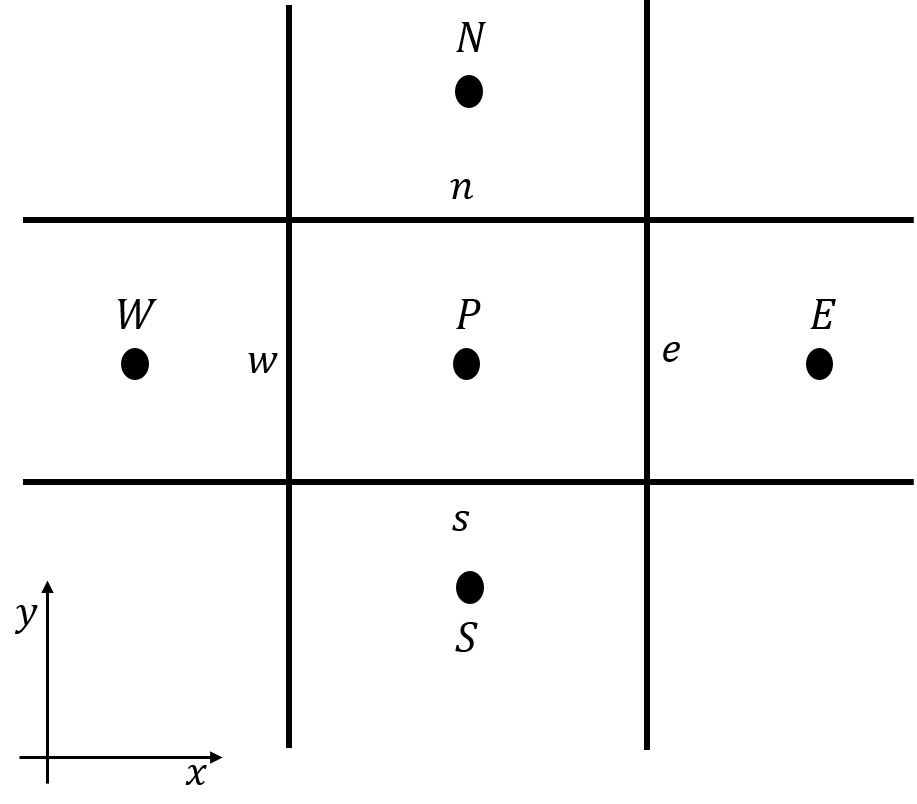
\includegraphics[width=0.4\textwidth]{ch2_litsurvey/Figures/2ddomainwaxisneigh.png}
\caption{$2D$ control volume around a node $P$.}
 \label{fig:2ddaxis}
\end{figure} 

The control volume is bound on four sides by faces $e$, $w$, $n$ and $s$  representing east, west, north and south respectively. Integrating equation~\ref{eq:genphi} on a control volume $\Omega$ gives
\begin{equation}
\int_{\Omega}\frac{\partial (\rho \phi)}{\partial t}d\Omega + \int_{\Omega} \frac{\partial (\rho U_i \phi)}{\partial x_i} d\Omega = \int_{\Omega}\frac{\partial}{\partial x_i}\left(\Gamma\frac{\partial \phi}{\partial x_i}\right) d\Omega + \int_{\Omega} Q d\Omega.
\label{eq:genphidisc}
\end{equation}

\subsubsection{Discretization of the viscous term}
First consider the diffusion term on the right hand side of equation~\ref{eq:genphidisc}. Using the divergence theorem the volume integral can be converted into a surface integral as
\begin{equation}
\int_{\Omega}\frac{\partial}{\partial x_i}\left(\Gamma\frac{\partial \phi}{\partial x_i}\right) d\Omega = \int_{\partial \Omega} \left(\Gamma\frac{\partial \phi}{\partial x_i}\right) n_i d (\partial\Omega),
\end{equation}
where $\partial \Omega$ represents the boundary of the control volume and $n_i$ is the unit outward pointing normal of the boundary. In the simplified $2D$ example of figure~\ref{fig:2ddaxis}, 
%the boundary of the control volume consists of the faces $e$, $w$, $n$ and $s$ and thus 
the integral can be written as a summation over the four faces as
\begin{equation}
\int_{\partial \Omega} \left(\Gamma\frac{\partial \phi}{\partial x_i}\right) n_i d (\partial\Omega) = \sum_{f} \left(\Gamma\frac{\partial \phi}{\partial x_i}\right) n_i \Delta S_f,
\end{equation}
where $f=e,w,n$ and $s$, $n_i$ is the corresponding outward unit normal vector of the face $f$ and $\Delta S_f$ is the area of the face $f$. Here the midpoint integration rule is used and the quantities on the face $f$ are computed at the face centroids. Based on the axis directions shown in figure~\ref{fig:2ddaxis} the summation can be expanded as
\begin{align}
\sum_{f} \left(\Gamma\frac{\partial \phi}{\partial x_i}\right) n_i \Delta S_f = \left(\Gamma\frac{\partial \phi}{\partial x_1}\right)_e \Delta S_e - 
\left(\Gamma\frac{\partial \phi}{\partial x_1}\right)_w \Delta S_w + \nonumber \\
\left(\Gamma\frac{\partial \phi}{\partial x_2}\right)_n \Delta S_n -
\left(\Gamma\frac{\partial \phi}{\partial x_2}\right)_s \Delta S_s.
\label{eq:viscsumm}
\end{align}
Here $x_1$ and $x_2$ are the $x$ and $y$ directions respectively. The derivatives at the faces can be written based on the nodal values of $\phi$. For example, considering the neighboring nodes to east of node $P$ in figure~\ref{fig:2ddaxis} to be $E$, the derivative of $\phi$ at the face $e$ for a constant $\Gamma$ can be written as
\begin{equation}
\left(\Gamma\frac{\partial \phi}{\partial x_1}\right)_e \Delta S_e = \Gamma \frac{\phi_E-\phi_P}{\Delta_{PE}}\Delta S_e = a_{E,v}\phi_E - a_{E,v}\phi_P,
\end{equation}
where $\Delta_{PE}$ is the distance between the nodes $P$ and $E$ and $a_{E,v}$ is the viscous coefficient of $\phi_E$ given by
\begin{equation*}
a_{E,v} = \Gamma \frac{\Delta S_e}{\Delta_{PE}}.
\end{equation*}
Similar expressions can be written for the other terms in the summation in equation~\ref{eq:viscsumm} to obtain an algebraic relation in terms of the nodal values of $\phi$ with the viscous coefficients being
\begin{equation*}
a_{W,v} = \Gamma \frac{\Delta S_w}{\Delta_{PW}}, \quad a_{N,v} = \Gamma \frac{\Delta S_n}{\Delta_{PN}}, \quad a_{S,v} = \Gamma \frac{\Delta S_s}{\Delta_{PS}},
\end{equation*}
and
\begin{equation*}
a_{P,v} = -(a_{E,v} + a_{W,v} + a_{N,v} + a_{S,v}).
\end{equation*}
Here $a_{P,v}$ is the viscous coefficient of $\phi_{P}$.
\subsubsection{Discretization of the advective term}
Now focusing on the advective term of equation~\ref{eq:genphidisc} and applying the divergence theorem again gives,
\begin{equation}
\int_{\Omega} \frac{\partial (\rho U_i \phi)}{\partial x_i} d\Omega = \int_{\partial \Omega} \rho U_i \phi n_i d(\partial \Omega).
\end{equation}
Similar to the discretization of the viscous term, the surface integral can be split into a summation over the four bounding faces of the control volume shown in figure~\ref{fig:2ddaxis}
\begin{equation*}
\int_{\partial \Omega} \rho U_i \phi n_i d(\partial \Omega) = \sum_f \left(\rho U_i \phi n_i \right)_f \Delta S_f,
\end{equation*}
\begin{equation*}
\sum_f \left(\rho U_i \phi n_i \right)_f \Delta S_f = \left(\rho U_1 \phi \right)_e \Delta S_e - \left(\rho U_1 \phi \right)_w \Delta S_w + \left(\rho U_2 \phi \right)_n \Delta S_n - \left(\rho U_2 \phi \right)_s \Delta S_s,
\end{equation*}
where the same sign convention used for the viscous discretization is also applied here and the mid point integration rule is used to approximate the integral over the face. The  term within the brackets can be found using the known velocity field. Determining the value of the scalar variable, $\phi$, can be done in various ways. Some of the more common methods are described below.
\begin{figure}[h]
\centering
\captionsetup{justification=centering}
 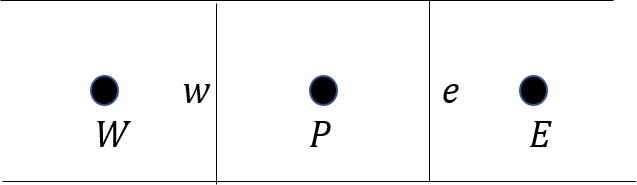
\includegraphics[width=0.3\textwidth]{ch3_su2eqn/figures/1dcv.png}
\caption{$1D$ control volume around node $P$ and neighboring nodes $E$ and $W$.}
 \label{fig:ch2pefrcinterp}
\end{figure}
\paragraph{Central scheme}
In a central scheme, the value of the scalar variable is approximated as the weighted average of the neighboring nodes. For example at the face $e$ and assuming the eastward neighbor of node $P$ in figure~\ref{fig:ch2pefrcinterp} is $E$, the value of $\phi$ is simply
\begin{equation}
\phi_e = \lambda_P \phi_P + \lambda_E \phi_E,
\end{equation}
where $\lambda_P$ and $\lambda_E$ are weighting factors of $P$ and $E$ respectively given by
\begin{equation}
\lambda_P = \frac{d_{Pe}}{d_{PE}}, \quad \lambda_E = \frac{d_{eE}}{d_{PE}}.
\end{equation} 
Here $d_{Pe}$ is the distance from node $P$ to face $e$, $d_{eE}$ is the distance from face $e$ to node $E$ and $d_{PE}$ is the distance from node $P$ to node $E$ ($d_{PE} = d_{Pe} + d_{eE}$). Thus, the contribution from the face $e$ to the summation can be written in terms of the nodal values of $\phi$ as 
\begin{equation}
\left(\rho U_i \phi \right)_e \Delta S_e = (\rho U_1 \Delta S)_e \lambda_P \phi_P + (\rho U_1 \Delta S)_e\lambda_E \phi_E.
\end{equation}
Hence,
\begin{equation*}
a_{E,c} = (\rho U_1 \Delta S)_e\lambda_E.
\end{equation*}
Similarly for the other faces around the control volume of node $P$ in figure~\ref{fig:2ddaxis}, the coefficients of the nodal values of $\phi$ can be written as
\begin{equation*}
a_{W,c} = -(\rho U_1 \Delta S)_w\lambda_W, \quad a_{N,c} = (\rho U_2 \Delta S)_n\lambda_N, \quad a_{S,c} = -(\rho U_2 \Delta S)_s\lambda_S,
\end{equation*}
and as with the viscous term discretization,
\begin{equation*}
a_{P,c} = -(a_{E,c} + a_{W,c} + a_{N,c} + a_{S,c}).
\end{equation*}
\paragraph{Upwind scheme}
An alternative to the central scheme, is to mimic the physics of the problem and determine the value at the face based on the direction of flow. 
Denoting the term
\begin{equation*}
\rho U_i n_i \Delta S_f = \dot{m}_f,
\end{equation*}
as the mass flux across the face $f$, the direction of the flow can be found based on the sign of the mass flux. Choosing the value of $\phi$ as
\begin{equation}
\phi_e = \begin{cases}
\phi_P\quad if\quad \dot{m}_e > 0, \\
\phi_E\quad if\quad \dot{m}_e < 0,
\end{cases}
\end{equation}
will replicate the physics of the flow at the face $e$. If the flow is in the positive $x$ direction, the mass flux at the face $e$ is positive ($\dot{m}_e>0$) and the value of the variable at the node $P$ is chosen. On the other hand if the direction of the flow is reversed, the value of $\phi$ at the node $E$ is chosen. This ensures the physics of the flow is also replicated in the discretized equation. The coefficients of the nodal values of $\phi$ for the face $e$ are then
\begin{equation}
a_{E,c} = \text{max}(-m_e,0.0), \quad a_{P,c} = \text{max}(m_e,0.0).
\end{equation}
Similar expressions can be written at other faces to find the coefficients of $\phi_P$ and its neighbors.

To examine the difference in behavior of the central and upwind scheme, consider a one dimensional pure advection problem given by
\begin{equation}
\frac{\partial \rho \phi}{\partial t} + \frac{\partial (\rho U \phi)}{\partial x} = 0.
\label{eq:advecphieqn}
\end{equation}
Let the domain of the problem be $x \in [0,1]$ and $U=1$ is the advection velocity and $\rho=1$ is the density. Assume an initial condition for $\phi$ as
\begin{equation}
\phi_0 = \begin{cases}
1.0 \quad if \quad x < 0.25, \\
0 \quad if \quad x > 0.25.
\end{cases}
\end{equation}
Since no dissipation is present, the initial condition must be advected across the domain without any loss in information. Figure~\ref{fig:upwcen} shows the numerical results from both the upwind and central schemes compared against the exact solution.
\begin{figure}[h]
\centering
\captionsetup{justification=centering}
 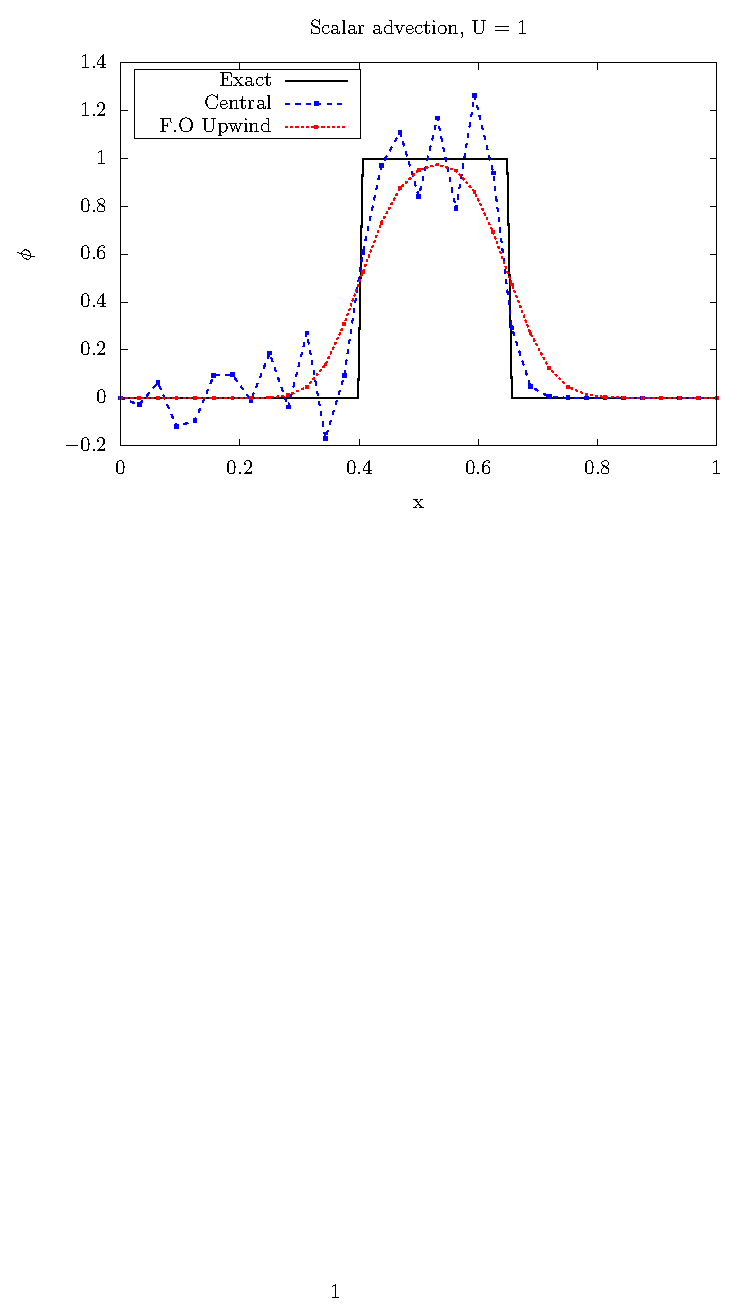
\includegraphics[trim=0 390 0 0,clip, width=0.5\textwidth]{ch2_litsurvey/Figures/box_cen_fo.eps}
\caption{Comparison of numerical solutions and exact solution for one dimensional scalar advection equation using central and first order upwind schemes.}
 \label{fig:upwcen}
\end{figure}
In this case, a uniform grid with $128$ elements was used. The solution shown is at time $t=0.5$. While the central scheme is more accurate, it is prone to instability which can be seen in the form of the unphysical wiggles that appear around the exact solution. This is understandable since the central discretization does not take the physics of the flow into account. However, while the upwind scheme does not have any wiggles in the solution, there is a loss of information and thus it is not very accurate. The source of these errors can be found by analyzing the truncation errors due for the upwind and central schemes~\cite{Moukalled, Ferziger2002}. Expanding the value of $\phi_f$ around the upwind node $U$ using Taylor series
\begin{equation}
\phi_f = \phi_U + \left(\frac{\partial \phi}{\partial x}\right)_U\Delta x + + \frac{1}{2!}\left(\frac{\partial^2 \phi}{\partial x^2}\right)_U\Delta x^2 + ...
\end{equation}
where $\Delta x$ is the distance between the upwind node $U$ and the face $f$. The upwind discretization presented so far only uses the first term in this expansion. The first term where the approximation gets truncated is a function of $\Delta x$ and thus this scheme is said to be first order accurate. In order to improve the accuracy of the upwind scheme the value at the face can be improved by considering more terms of the Taylor series expansion.
\paragraph{Second order upwind}
Instead of using only the value at the upstream node, the approximation of the face value of $\phi$ can be improved if the gradient of $\phi$ at the upstream node is also used. The value of $\phi$ at a face $f$ is reconstructed using both the value of $\phi$ at the upstream node and its gradient as
\begin{equation*}
\phi_f = \phi_U + \left(\frac{\partial \phi}{\partial x}\right)_U\Delta x,
\end{equation*}
where $f$ is the face under consideration, $U$ denotes the upstream node and $\Delta x$ is the distance from the node $U$ to the face $f$. In this approximation, the truncation error is of the order ($\Delta^2$) and the value is second order accurate. The solution of the one dimensional pure advection equation using the second order upwind scheme is shown in figure~\ref{fig:upwcen2ord}.
\begin{figure}[h]
\centering
\captionsetup{justification=centering}
 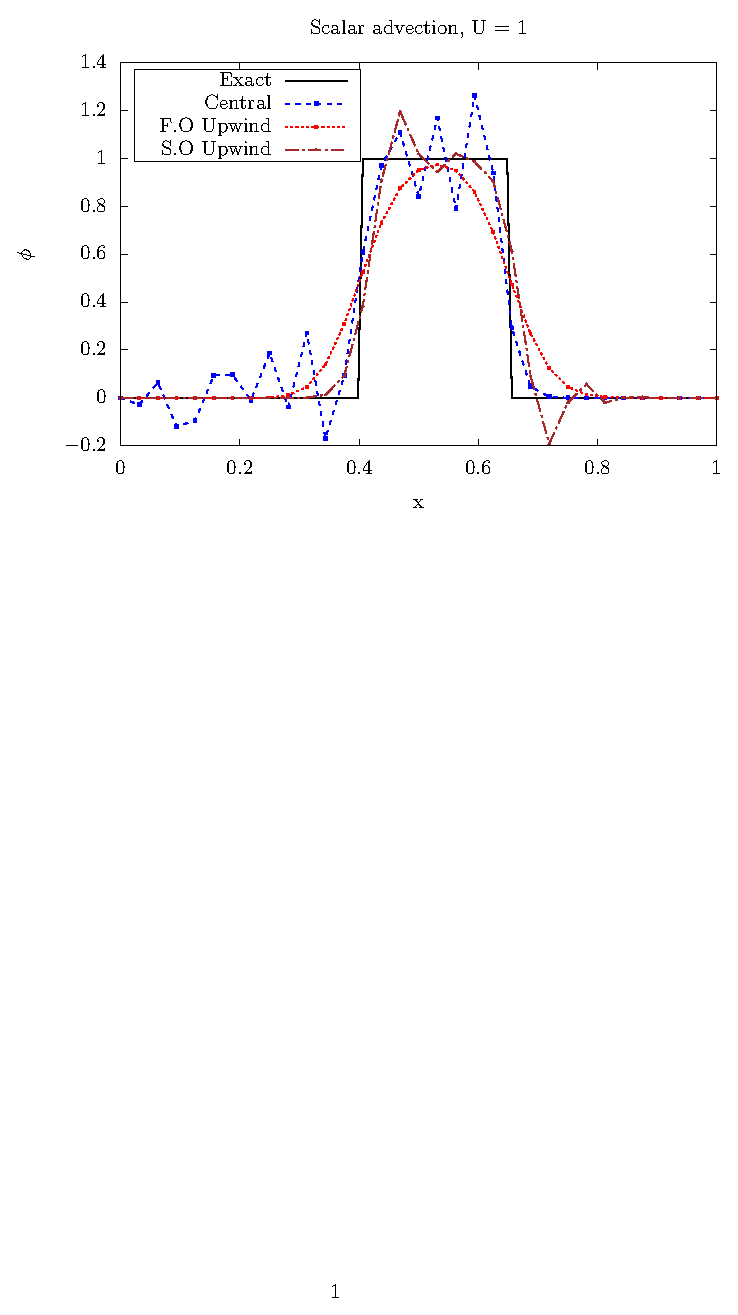
\includegraphics[trim=0 395 0 0,clip, width=0.5\textwidth]{ch2_litsurvey/Figures/box_cen_foso.eps}
\caption{Comparison of numerical solution and exact solution for one dimensional scalar advection equation using central, first and second order upwind schemes.}
 \label{fig:upwcen2ord}
\end{figure}
Clearly, there is less loss of information compared to the first order approximation and there are fewer wiggles than the central discretization.
\paragraph{Slope limiters}
However, reconstructing the face value using gradients can also lead to non-physical oscillations and convergence issues at times. This can be seen in figure~\ref{fig:upwcen2ord} at the end of the wave. A monotonic upwind discretization can be found based on the concept of total variation~\cite{hirsch1997numerical}. The total variation of $\phi$ in equation~\ref{eq:advecphieqn} is given by
\begin{equation}
TV = \int\left|\frac{\partial \phi}{\partial x}\right|dx.
\end{equation}
The total variation of any physically admissible solution does not increase in time~\cite{hirsch1997numerical,leveque2002finite}. A numerical scheme can produce a physically monotonic solution only if it ensures that the total variation of the solution does not increase. Such schemes are called Total Variation Diminishing (TVD) schemes. Based on the concept of total variation, slope limiters that ensure the solution remains smooth and monotonic near sharp gradients can be derived~\cite{hirsch1997numerical,leveque2002finite}. The value of $\phi$ at a face $f$ is reconstructed using slope limiters, given by
\begin{equation*}
\phi_f = \phi_U + \psi(r)\left(\frac{\partial \phi}{\partial x_i}\right)_U\Delta x,
\end{equation*}
where $f$ is the face under consideration, $U$ denotes the upstream node, $\Delta x$ is the distance from the node $U$ to the face $f$ and $\psi(r)$ is the slope limiter function. For the face $e$ in figure~\ref{fig:ch2pefrcinterp}, $r$ is given by
\begin{equation*}
r = \frac{u_P - u_W}{u_E - u_P}.
\end{equation*}
For the van Albada~\cite{vanalbada} slope limiter, $\psi(r)$ is given by
\begin{equation*}
\psi(r) = \frac{r^2 + r}{r^2 + 1}.
\end{equation*}
The solution of the $1D$ scalar advection equation using the van Albada slope limiter is shown in figure~\ref{fig:slopelim}.
\begin{figure}[h]
\centering
\captionsetup{justification=centering}
 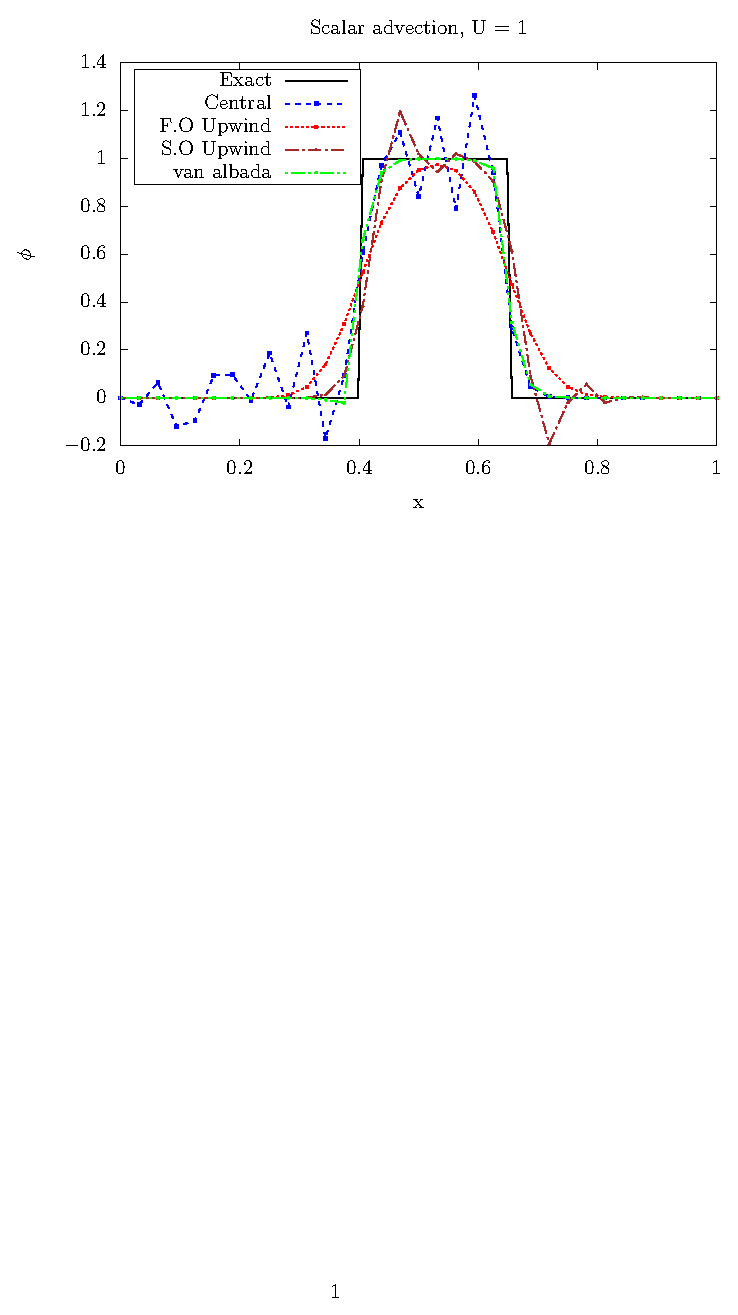
\includegraphics[trim=0 395 0 0,clip, width=0.5\textwidth]{ch2_litsurvey/Figures/box_cen_fososl.eps}
\caption{Comparison of numerical solution and exact solution for one dimensional scalar advection equation using central, first, second order upwind schemes with and without slope limiter.}
 \label{fig:slopelim}
\end{figure}
With the use of the van Albada slope limiter, a more accurate representation of the exact solution is found without any oscillations.
%\subsubsection{QUICK}
\subsubsection{Discretization of the source term}
The source term, $Q$, can be discretized using the mid point integration rule. For example on a control volume around a node $P$ shown in figure~\ref{fig:2ddaxis}, the discretized form of the source term is
\begin{equation}
\int_{\Omega} Q d\Omega \approx Q_P |\Omega| = b_P.
\end{equation}
This discretization is approximately second order accurate~\cite{Ferziger2002}.

\subsubsection{Discretized equation}
The semi discretized form of equation~\ref{eq:genphidisc} for a node $P$ can be written as
\begin{equation}
\int_{\Omega} \frac{\partial \phi}{\partial t} d\Omega + a_P \phi_P + \sum_{C\in\mathcal{N}(P)}a_{C}\phi_{C} = b_P,
\label{eq:algeqnphist1}
\end{equation}
where $C\in\mathcal{N}(P)$ denotes the neighbors of the node $P$ and $b_P$ is the discretized source term contribution. The coefficients, $a$, are the sum of the advective and viscous contributions
\begin{equation*}
a_P = a_{P,c} + a_{P,v}, \quad a_{C} = a_{C,c} + a_{C,v}.
\end{equation*}
%The discretization of the unsteady term will now be described. 

\subsubsection{Time discretization}
Finally, focusing on the unsteady term in equation~\ref{eq:genphidisc} and using the mid point rule for a control volume around a node $P$ as shown in figure~\ref{fig:2ddaxis} gives,
\begin{equation}
\int_{\Omega} \frac{\partial \phi}{\partial t} d\Omega \approx \frac{\partial \phi}{\partial t} |\Omega|_P.
\end{equation}
The time derivative can be discretized in different ways. The simplest method is to use the Euler time integration schemes. Denoting quantities at a time level $t^n$ as $\phi^n$, the approximation for the unsteady term is
\begin{equation}
\frac{\partial \phi}{\partial t} |\Omega|_P \approx \frac{\phi^{n+1}_P - \phi^n_P}{\Delta t} |\Omega|_P.
\end{equation}
There are now two possible approaches to solve equation~\ref{eq:algeqnphist1}. Either all the $\phi$ values in the spatially discretized terms could be from the current time level $t^n$ giving an explicit formulation or these values could be from the time level $t^{n+1}$ giving an implicit formulation.
\paragraph{Explicit Euler}
Using the known values of $\phi^n$ in the spatial discretization gives
\begin{equation}
\frac{\phi^{n+1}_P - \phi^n_P}{\Delta t} |\Omega|_P + a_P \phi_P^n + \sum_{C\in\mathcal{N}(P)}a_{C}\phi_{C}^n = b_P^n.
\end{equation}
The only unknown quantity in this equation is $\phi^{n+1}$ and this equation can be written in an explicit form to solve for $\phi^{n+1}$ as
\begin{equation*}
\phi^{n+1}_P = \phi^n_P + \frac{\Delta t}{|\Omega|_P}\left(b_P - a_P \phi_P^n - \sum_{C\in\mathcal{N}(P)}a_{C}\phi_{C}^n\right),
\end{equation*}
or 
\begin{equation}
\phi^{n+1}_P = \phi^n_P - \frac{\Delta t}{|\Omega|_P} R^n_P(\phi),
\end{equation}
where $R^n(\phi)_P$ is the residual at the time level $t^n$ given by
\begin{equation}
R^n_P(\phi) = a_P \phi_P^n + \sum_{C\in\mathcal{N}(P)}a_{C}\phi_{C}^n - b_P.
\end{equation}
\paragraph{Implicit Euler}
Using the values of $\phi$ from time level $t^{n+1}$ instead in equation~\ref{eq:algeqnphist1} gives
\begin{equation}
\frac{\phi^{n+1}_P - \phi^n_P}{\Delta t} |\Omega|_P + a_P \phi_P^{n+1} + \sum_{C\in\mathcal{N}(P)}a_{C}\phi_{C}^{n+1} = b_P^{n}.
\end{equation}
Thus, an implicit equation for $\phi^{n+1}_P$ is obtained, namely
\begin{equation*}
\phi^{n+1}_P \frac{|\Omega|_P}{\Delta t} + a_P \phi_P^{n+1} + \sum_{C\in\mathcal{N}(P)}a_{C}\phi_{C}^{n+1} = b_P^{n} + \phi^n_P \frac{|\Omega|_P}{\Delta t},
\end{equation*}
which can be further simplified as
\begin{equation}
a_P^t \phi_P^{n+1} + \sum_{C\in\mathcal{N}(P)}a_{C}\phi_{C}^{n+1} = B_P,
\label{eq:algeqnphiv1}
\end{equation}
where the coefficient $a_P^t$ contains the contribution from the spatial discretization as well as temporal discretization and the source term $B_P$ contains the contribution from the previous time step
\begin{equation}
a_P^t = a_P + \frac{|\Omega|_P}{\Delta t}, \quad B_P = b_P^{n} + \phi^n_P \frac{|\Omega|_P}{\Delta t}. 
\end{equation}

Alternately if only a steady state solution is required, using the residual $R_P(\phi)$ defined earlier, but now at the time level $t^{n+1}$ the above equation can be simplified as
\begin{equation}
\frac{\phi^{n+1} - \phi^n}{\Delta t} |\Omega|_P + R^{n+1}_P(\phi) = 0.
\label{eq:235}
\end{equation}
Instead of solving for $\phi^{n+1}$ directly, the numerator of the time discretization can be written as the update to the solution, $\Delta \phi^n = \phi^{n+1} - \phi^n$, at time level $t^n$. Thus, the equation~\ref{eq:235} can also be written as 
\begin{equation}
\frac{\Delta \phi^n}{\Delta t} |\Omega|_P + R^{n+1}_P(\phi) = 0.
\label{eq:implaltform}
\end{equation}
The residual $R^{n+1}_P(\phi)$ is also unknown and can be linearized about the time $t^n$ as 
\begin{equation*}
R_P^{n+1}(\phi)  = R_P^n(\phi) + \frac{\partial R_P^n}{\partial t}\Delta t + \mathcal{O}(\Delta t^2),
\end{equation*}
or 
\begin{equation}
R_P^{n+1}(\phi)  = R_P^n(\phi) + \sum_{C\in\mathcal{N}(P)}\frac{\partial R_P^n(\phi)}{\partial \phi_{C}}\Delta \phi^n_{C} + \mathcal{O}(\Delta t^2).
\end{equation}
The term $ \sum_{C\in\mathcal{N}(P)}\frac{\partial R_P^n(\phi)}{\partial \phi_{C}}$ is known as the Jacobian matrix. Thus equation~\ref{eq:implaltform} can be written as
\begin{equation}
\frac{\Delta \phi^n}{\Delta t} |\Omega|_P + \sum_{C\in\mathcal{N}(P)}\frac{\partial R_P^n(\phi)}{\partial \phi_{C}}\Delta \phi^n_{C} = -R_P^n(\phi).
\end{equation}
This can also be written in the form of equation~\ref{eq:algeqnphiv1} as 
\begin{equation}
a_P^{t^\prime} \phi_P + \sum_{C\in\mathcal{N}(P)}a_{C}^{\prime}\phi_{C} = B_P^{\prime},
\label{eq:algeqnphiv2}
\end{equation}
However, the coefficients are now different, namely
\begin{equation}
a_P^{t^\prime} = a_P^{\prime} + \frac{|\Omega|_P}{\Delta t}, \quad B_P^{\prime} = -R_P^n(\phi). 
\end{equation}
Here $a_P^{t,\prime}$ contains the coefficients of node $\phi_P$ from the Jacobian matrix and $a_{\mathcal{N}(P)}^{\prime}$ contains the coefficients of the neighbors of node $\phi_P$ from the Jacobian matrix.

So far it has been assumed that the coefficients of nodal values of $\phi$, $a_P$ are constant. This is true for the general scalar conservation equation (equation~\ref{eq:genphi}) with constant velocity field $U$. However, if the velocity field is itself not constant, the coefficients $a_P$ are evaluated using values at the time level $t^n$. 

\paragraph{System of linear algebraic equations}
The equation~\ref{eq:algeqnphiv1} or equation~\ref{eq:algeqnphiv2} can be written as a system of linear algebraic equations with the unknowns as the nodal values of $\phi$ as
\begin{equation}
\mathbf{A}_{ij}\phi_j = b_i,
\end{equation}
where $\mathbf{A}_{ij}$ is the coefficient matrix, $\phi_j$ is the vector of all the nodal values of $\phi$ and $b_i$ is the right hand side (RHS).
This equation can be solved using different linear solvers for which information can be found in literature~\cite{Moukalled,Ferziger2002,van2003iterative, strang1993introduction, saad1986gmres}. The linear solvers available in SU2 are the Flexible Generalized Minimal Residual (FGMRES)~\cite{saad1986gmres} and Biconjugate Gradient Stabilized (BiCGSTAB)\cite{van2003iterative, strang1993introduction, saad1986gmres} which will also be used in the pressure based solver.
%Before applying the solution procedure described here to solve the incompressible flow equations, the nature of the incompressible Navier Stokes equation will be examined.

In this section, the procedure to solve a generic partial differential equation of the form equation~\ref{eq:genphi} was described. The momentum equations (equation~\ref{eq:momindx}) closely resemble the generic conservation equation and the discretization described here can be used to solve them. However, when dealing with incompressible flows additional complications arise which will be described next.

\section{Pressure velocity coupling}
For an incompressible flow, the main variables of interest are the velocities, $u_i$ and pressure $p$ (\textit{primitive variables}). The momentum equations (equation~\ref{eq:momindx}) closely resemble the general scalar equation~\ref{eq:genphi}. However, unlike the scalar equation the velocity field is unknown and thus the equations are non linear. Additionally, it can be seen that the pressure, which is also unknown, appears as a gradient term in the momentum equations but the continuity equation (equation~\ref{eq:contindx}) does not contain pressure and cannot be used to solve for it. Thus, despite having four equations for the four unknowns, a direct solution is not possible from the system of equations. This pressure velocity coupling is the biggest challenge in solving the incompressible flow equations~\cite{Kwak2003,KWAK2005283, Ferziger2002, Moukalled, Shyy1994}. For compressible flow problems, the continuity equation acts as an evolution equation for density which can be used in conjunction with the energy equation and thermodynamic relations to obtain the pressure field. However as the continuity equation reduces to a divergence condition on the mass flux for incompressible flows and the energy equation is decoupled there is no direct way to compute the pressure field. 

A conceptual interpretation of this scenario would be to consider the implications of the constant density assumption. In any medium, sound travels as pressure and density disturbances. Since density is assumed to be a constant, the speed at which the pressure disturbances must travel is infinite. Thus the effect of any pressure disturbance is felt instantaneously everywhere in the domain. Realistically however, the speed of sound is many times faster than the reference velocities encountered in incompressible problems. This leads to the commonly used condition on the Mach number, $Ma < 0.3$, to determine if a flow is incompressible or not. The Mach number is a non-dimensional number and is defined as the ratio of the reference velocity, $V$, and the speed of sound, $c$. Thus at lower Mach numbers the speed of sound is much greater than the reference velocity and pressure disturbances can be assumed to travel much faster than the flow velocity.

This discrepancy in the different propagation speeds of pressure and velocity is reflected in the different natures of the governing equations. Pressure behaves in an elliptic manner propagating in all directions simultaneously and instantly, whereas the velocities behave in a parabolic manner i.e. have a definite marching direction~\cite{Ferziger2002}. In order to solve the incompressible flow equations, the two different natures of the pressure and velocity must be resolved.

\section{Solution methods}\label{ssec:pbdb}
One way to overcome the challenges posed by the incompressible form of the Navier Stokes equations is to solve the compressible Navier Stokes equations as they are also valid for incompressible flows. However there are many known drawbacks of this approach. The equations become very stiff at lower Mach numbers leading to poor convergence behavior. Additionally, the excessive numerical diffusion causes a degradation in the accuracy of the solutions~\cite{Tom2019,barsukow2017numerical}. Preconditioning of the compressible Navier Stokes equations~\cite{turkel1987preconditioned} can be used to overcome some of the limitations posed by solving the compressible equations, but such methods are more commonly used in flows where a wide range of Mach numbers are observed.

To alleviate the problems with pressure velocity coupling in the incompressible Navier Stokes equations, the pressure can be eliminated from the equations using derived quantities like stream function and vorticity~\cite{hirsch1997numerical, Ferziger2002} which can then be solved to obtain the flow field. In $2D$, the stream function, $\psi$, and vorticity, $\omega$, are related to the velocities $u$ and $v$ as
\begin{equation}
u = \frac{\partial \psi}{\partial y}, \quad v = -\frac{\partial \psi}{\partial x}
\end{equation}
and
\begin{equation}
\omega = \frac{\partial u}{\partial y} - \frac{\partial v}{\partial x}.
\end{equation}
Based on these definitions, a Poisson equation for the streamfunction and a conservation equation for vorticity can be found~\cite{Ferziger2002}. The nature of the two equations reflect the nature of pressure and velocity but the biggest advantage is that the pressure is eliminated as a dependent variable. However, there are some major drawbacks as well. It is difficult to specify boundary conditions for the stream function and vorticity, especially for complex geometries. Also this method does not generalize well into $3D$ as both vorticity and stream function have three components and thus there are six equations to be solved. 

Therefore, the use of the primitive variables (pressure and velocity) is preferred. There are two broad classes of methods to resolve the pressure velocity coupling in primitive variables: the density based approach and the pressure based approach.

%The continuity equation (equation~\ref{eq:contindx}) is automatically satisfied when the velocities are written in terms of the streamfunction. Additionally, substituting the velocities in terms of streamfunction in the definition of vorticity gives a Poisson equation of the form
%\begin{equation}
%\frac{\partial^2 \psi}{\partial x^2} + \frac{\partial^2 \psi}{\partial y^2} = -\omega.
%\end{equation}
%Diffrentiating the $x$ and $y$ momentum equations with respect to $y$ and $x$ respectively and subtracting them, an equation for vorticity can be written as

%\subsection{Density based approach}
An example of the density based method is the pseudo compressibility approach~\cite{Park1984, Kwak2003, chorinartcomp} where  an artificial speed of sound is introduced in the continuity equation to mimic the compressible flow formulation.  The most common approach, especially for constant density flows, is to introduce a time derivative of the pressure in the continuity equation to transform the behavior of the continuity equation from elliptic to hyperbolic. Equation~\ref{eq:contindx} is then becomes
\begin{equation}
\frac{1}{\beta}\frac{\partial p}{\partial t} + \frac{\partial u_i}{\partial x_i} = 0.
\label{eq:artcompbeta}
\end{equation}
Here $\beta$ is the artificial compressibility factor. The larger the value of $\beta$, the closer the equation~\ref{eq:artcompbeta} is to the incompressible equations. Clearly, equation~\ref{eq:artcompbeta} is not time accurate and is valid only for steady state problems. A dual time stepping algorithm can overcome this limitation. The artificial compressibility factor, $\beta$ can be considered as a form of preconditioning for the continuity equation. Its value will have a marked effect on the convergence behavior of the solution. For steady state problems, it can affect the accuracy of the solution via artificial dissipation. This method belongs to the more general approach of pre-conditioned compressible flow solution methods. Economon~\cite{Tom2019} suggests to precondition all the equations instead of only the continuity equation for robustness and stability of the solver.

The existing incompressible solver in SU2 follows this approach and has been extended to variable-density flows and heat transfer applications~\cite{Tom2019}. The aim of this thesis is to implement a pressure based solver in SU2. The details of such a solver will be given in the next section.
%\subsection{Pressure based approach}

\section{Pressure based methods}

The difficulty in solving the incompressible equations was explored qualitatively earlier. Numerically it manifests as the well known checkerboard pressure problem~\cite{Patankar1980,Moukalled}. This problem arises from the discretization of the pressure gradient term in the momentum equations. 
\begin{figure}[h]
\centering
\captionsetup{justification=centering}
 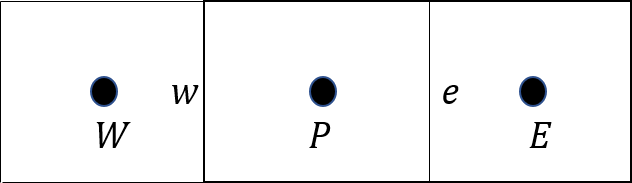
\includegraphics[width=0.3\textwidth]{ch2_litsurvey/Figures/1ddomain.png}
\caption{One dimensional control volumes around nodes $P$ and the neighboring nodes$E$ and $W$.}
%across a face $e$.}
 \label{fig:1dCV}
\end{figure}
If the pressure gradient is treated as a source term and integrated using the mid point rule over the control volume like the one shown in figure~\ref{fig:1dCV}, the discretized form can be written as 
\begin{equation}
\int_{\Omega} \frac{\partial p}{\partial x_i} d\Omega \approx \frac{\partial p}{\partial x_i}|\Omega|.
\end{equation}
In the simplified one dimensional scenario, for the control volume around a node $P$ with two neighbors $E$ and $W$ to the east and west respectively (figure~\ref{fig:1dCV}), using a central difference scheme the discretized form reduces to 
\begin{equation}
\frac{\partial p}{\partial x_i}|\Omega| = \frac{p_E - p_W}{2\Delta x}|\Omega|.
\end{equation}
A uniform grid spacing of $\Delta x$ is assumed throughout the domain for simplicity. Thus, the discretized pressure gradient term involves only the difference between alternating nodes. Similarly, the continuity equation
\begin{equation}
\frac{\partial u_i}{\partial x_i} = 0
\end{equation}
which discretized in a one dimensional scenario for a control volume around node $P$ is simply
\begin{equation}
\int_{\Omega}\frac{\partial u}{\partial x} d\Omega \approx (u_e - u_w)\Delta S = 0.
\end{equation}
Using the central scheme gives
\begin{equation}
u_E - u_W = 0.
\end{equation}
Once again, the discretized equation around a node $P$ relies only on alternating nodes. Under such conditions any zigzag pressure field will appear uniform and a zigzag velocity field will satisfy the continuity equation. Additionally, if a certain pressure field is found as the solution, infinitely more solutions can be found by adding an arbitrary zigzag variation to the smooth solution.

\subsection{Staggered grids}\label{sec:pcorrstag}
Since the pressure terms in the discretized momentum equation was decoupled from the velocity, one potential solution is to stagger the locations where pressure and velocities are computed. In a staggered arrangement, the velocities are stored at the cell faces and pressure is stored at the centroid. In two dimensions, the $x$ component of the velocity is staggered in the $x$ direction and the $y$ component of the velocity is staggered in the $y$ direction as seen in figure~\ref{fig:stagger}. 
\begin{figure}[h!]
\centering
\captionsetup{justification=centering}
 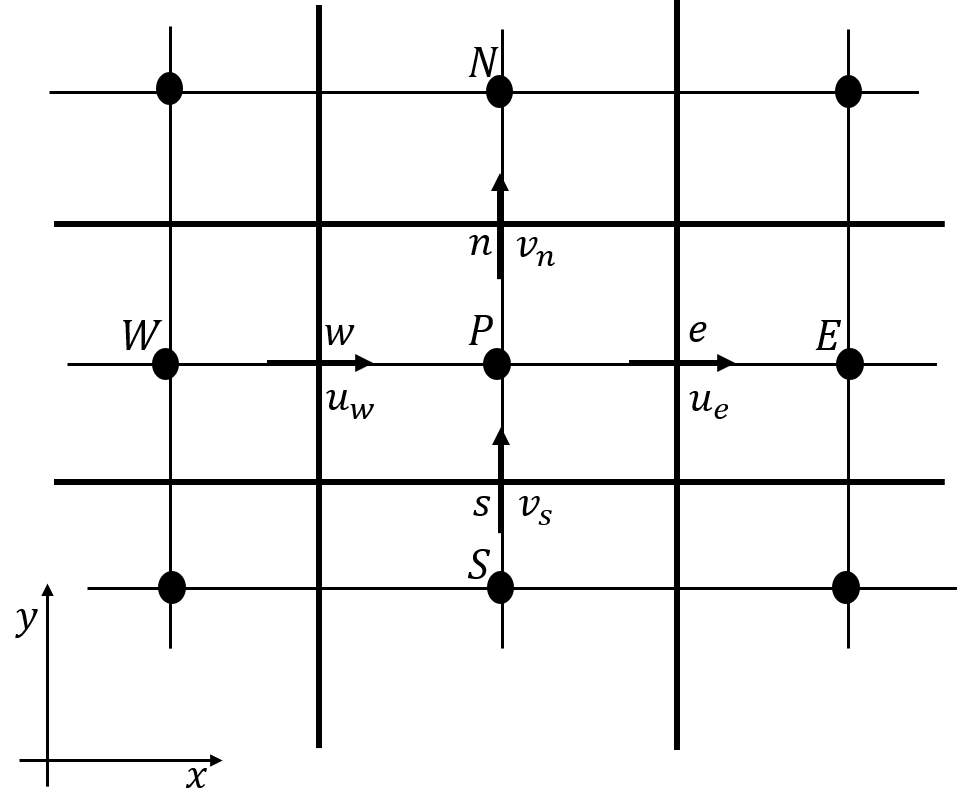
\includegraphics[width=0.5\textwidth]{ch2_litsurvey/Figures/stag2ddomain.png}
\caption{Staggered grid showing the locations of pressure and velocity variables in $2D$.}
 \label{fig:stagger}
\end{figure}

This scheme was first suggested by Harlow and Welch~\cite{F.H.Harlow1965} in their marker and cell (MAC) method. One consequence of storing the velocities and pressure at staggered locations is that the control volumes for each of the momentum and continuity equations is now different. In figure~\ref{fig:stagger}, the control volume for the continuity equation is formed around node $P$, for the momentum equation in $x$ direction, the control volume is formed around the mid point of face $e$ (or $w$) and for the momentum equation in $y$ direction the control volume is formed around the mid point of face $n$ (and $s$).
The pressure gradient term in the momentum equations can be computed directly based on cell values. Also, there is no need to interpolate velocities to the faces since they are available directly. The momentum equations for the velocity components can be solved in a segregated manner treating each of them similar to the scalar equation~\ref{eq:genphi}. For example, the equation for the $x$ component of velocity on the face $e$ in figure~\ref{fig:stagger} will be
\begin{equation}
a_e^u u_e + \sum_{f \in\mathcal{N}(e)} a_f^u u_f = -|\Omega|_e \frac{\partial p}{\partial x_e},
\label{eq:segueqn}
\end{equation}
where $a_e^u$ is the coefficient of $u$ at the face $e$, $a_f$ are the coefficients of the neighboring nodes $\mathcal{N}(e)$. The coefficients can be found as described in section~\ref{sec:ch2disceqnphi}. However, unlike the scalar transport equation since the velocity field itself is unknown, the coefficients are a function of the velocities. The pressure gradient term is treated as a constant within the control volume. The gradient can now be found as 
\begin{equation}
\frac{\partial p}{\partial x} = \frac{p_E - p_P}{\delta x_{PE}},
\end{equation}
which can be found without any interpolation since the pressure values are stored on the nodes $P$ and $E$. Since consecutive nodes are used to find the pressure gradient, the checkerboard problem is eliminated. However, the value of the pressure is not known and needs to be solved for simultaneously. At this stage, in order to find a new equation for the pressure, the divergence of the discretized momentum equations can be taken and along with the continuity equation a Poisson equation for the pressure can be found~\cite{Ferziger2002}. The most commonly used procedure to do this is described now.

Equation~\ref{eq:segueqn} can only be solved if the pressure is either known beforehand or at least estimated. If an estimate of the pressure field is used, the resulting velocity field will also be an estimate. Denoting the velocity estimate by an $\ast$, the equation~\ref{eq:segueqn} can be written more accurately as
\begin{equation}
a_e^u u_e^{\ast} + \sum_{f \in\mathcal{N}(e)} a_f^u u_f^{\ast} = -|\Omega|_e \frac{\partial p^{\ast}}{\partial x_e}.
\label{eq:segueqn*}
\end{equation}
Similarly, the estimate of pressure is represented by $p^{\ast}$. Denoting the corrections to velocities and pressure by $u_e^{\prime}$ and $p^{\prime}$, the corrected velocity and pressure are
\begin{equation}
p=p^{\ast} + p^{\prime}, \quad u_e = u_e^{\ast} + u_e^{\prime}.
\end{equation}
Subtracting equation~\ref{eq:segueqn*} from equation~\ref{eq:segueqn}, 
\begin{equation}
a_e^u u_e^{\prime} + \sum_{f \in\mathcal{N}(e)} a_f^u u_f^{\prime} = -|\Omega|_e \frac{\partial p^{\prime}}{\partial x_e}.
\label{eq:segueqncorr}
\end{equation}
Analogous equations can be written for the vertical component of the velocity at the face $n$ in figure~\ref{fig:stagger} as
\begin{equation}
a_n^v v_n^{\prime} + \sum_{f \in\mathcal{N}(n)} a_f^v v_f^{\prime} = -|\Omega|_n \frac{\partial p^{\prime}}{\partial y_n}.
\label{eq:segveqncorr}
\end{equation}

Unlike the momentum equations where the control volume for velocities are defined around cell faces (like $e$ in figure~\ref{fig:stagger}), the continuity equation is solved using the control volume around a node. In figure~\ref{fig:stagger}, the discretized continuity equation around the node $P$ is
\begin{equation}
\sum_f \dot{m}_f = \dot{m}_e + \dot{m}_w + \dot{m}_n + \dot{m}_s = 0.
\end{equation}
Since the velocities are stored at the faces, the mass fluxes can be written in terms of the face velocities directly as
\begin{equation}
\dot{m}_e = \rho u_e \Delta S_e = \rho u_e^{\ast} \Delta S_e + \rho u_e^{\prime} \Delta S_e = \dot{m}_e^{\ast} + \dot{m}_e^{\prime},
\end{equation}
where $\dot{m}_e^{\ast}$ and $\dot{m}_e^{\prime}$ is the estimated mass flux and the correction of the mass flux. The continuity equation in terms of the estimated and corrected mass flux is
\begin{equation*}
\sum_f (\dot{m}_f^{\ast} + \dot{m}_f^{\prime}) = 0,
\end{equation*}
or
\begin{equation}
\sum_f \dot{m}_f^{\prime} = -\sum_f \dot{m}_f^{\ast}.
\end{equation} 
Substituting for mass flux correction in terms of the velocity corrections
\begin{equation}
\rho u^{\prime}_e \Delta S_e - \rho u^{\prime}_w \Delta S_w + \rho u^{\prime}_n \Delta S_n - \rho u^{\prime}_s \Delta S_s  = -\sum_f \dot{m}_f^{\ast}.
\label{eq:contstag}
\end{equation}
The estimated mass flux can be computed from the solution of equation~\ref{eq:segueqn*}. Substituting for the velocity corrections from equation~\ref{eq:segueqncorr} will give a new equation for the pressure corrections which can be used to overcome the pressure velocity coupling. Patankar and Spalding~\cite{Patankar1972} introduced an additional simplification to equation~\ref{eq:segueqncorr} by neglecting the term $\sum_{f \in\mathcal{N}(e)} a_f^u u_f^{\prime}$ giving 
\begin{equation}
u_e^{\prime} = -\frac{|\Omega|_e}{a_e^u} \frac{\partial p^{\prime}}{\partial x_e}.
\label{eq:simplestageqn}
\end{equation}
Substituting this simplified equation of the velocity correction in equation~\ref{eq:contstag} results in
\begin{equation}
-\left(\rho \frac{|\Omega|_e}{a_e^u} \frac{\partial p^{\prime}}{\partial x_e} \Delta S_e - \rho\frac{|\Omega|_w}{a_w^u} \frac{\partial p^{\prime}}{\partial x_w} \Delta S_w + \rho \frac{|\Omega|_n}{a_n^v} \frac{\partial p^{\prime}}{\partial y_n} \Delta S_n - \rho \frac{|\Omega|_s}{a_s^v} \frac{\partial p^{\prime}}{\partial y_s} \Delta S_s\right)  = \sum_f \dot{m}_f^{\ast}.
\label{eq:pcorrstag1}
\end{equation}
Denote the coefficient of the pressure gradient terms as
\begin{equation}
D_f = \rho \frac{|\Omega|_f}{a_f} \Delta S_f,
\label{eq:ch2dfeqn}
\end{equation}
where $f$ is the face. Equation~\ref{eq:pcorrstag1} can then be written as
\begin{equation}
\sum_f -D_f \frac{\partial p^{\prime}}{\partial x_e} = \sum_f \dot{m}_f^{\ast}.
\label{eq:pcorrstag2}
\end{equation}
This equation is a discretized Poisson equation for the pressure correction. This pressure corrections will be used to correct the estimated pressure used in equation~\ref{eq:segueqn*}. 
%Equation~\ref{eq:simplestageqn} can then be used to find the velocity corrections. 

\subsubsection{Pressure and velocity corrections}
Once the pressure corrections are found by solving equation~\ref{eq:pcorrstag2}, the velocity corrections can be found from equation~\ref{eq:simplestageqn}
\begin{equation*}
u_e^{\prime} = -\frac{|\Omega|_e}{a_e^u} \frac{\partial p^{\prime}}{\partial x_e}.
\end{equation*}
With the pressure and velocity corrections, the estimated values can now be updated as follows
\begin{eqnarray}
p = p^{\ast} + \alpha_p p^{\prime}, \label{eq:pcorrstg}\\
u = u^{\ast} + u^{\prime}.\label{eq:ucorrstg}
\end{eqnarray}
Here $\alpha_p$ is an under-relaxation parameter for the pressure correction. At convergence, the estimated velocities will satisfy the continuity equation rendering the right hand side of the equation~\ref{eq:pcorrstag2} zero which then makes the pressure corrections and subsequently velocity corrections also go to zero. It is necessary to use some under-relaxation in pressure correction to ensure convergence~\cite{Ferziger2002, Moukalled, Patankar1972}. No under-relaxation is necessary for the velocity corrections.

\subsubsection{SIMPLE algorithm}
This procedure of using an estimate of the pressure field to find the velocity field using the momentum equations and then correcting both using the continuity equation is known as the Semi-Implicit Method for Pressure-Linked Equations or SIMPLE~\cite{Patankar1972, caretto1973two}. The solution algorithm is
\begin{enumerate}
    \item Guess the pressure field $p^{\ast}$.
    \item Solve the momentum equations like equation~\ref{eq:segueqn*} to find the estimated velocities $u_i^{\ast}$.
    \item Find the mass flux at the faces $m_f^{\ast}$ using the estimated velocities.
    \item Assemble the pressure correction equation based on the mass fluxes and the momentum equation.
    \item Solve the pressure correction equation (Eq. \ref{eq:pcorrstag2}) to find the pressure and velocity corrections.
    \item Update the pressure and velocity corrections using equations~\ref{eq:pcorrstg} and equation~\ref{eq:ucorrstg} and repeat till convergence.
\end{enumerate}
The biggest assumption made in this procedure was the neglection of the term $\sum_{f \in\mathcal{N}(e)} a_f^u u_f^{\prime}$ in equation~\ref{eq:segueqncorr}. This term contains the information about velocity corrections of the neighboring nodes. However, since the neglected terms are only used in the iterative pressure velocity correction algorithm, it does not have an effect on the final solution. It does however have an effect on the rate of convergence of the iterative procedure and occasionally whether the algorithm converges at all.

\subsubsection{SIMPLE family of algorithms}

There are many variants of the widely used SIMPLE algorithm~\cite{Patankar1980, Moukalled, Murthy2002, Xiao2018, pisoref, simplerref} that can improve the performance.
\paragraph{SIMPLEC}
Instead of neglecting the term $\sum_{f \in\mathcal{N}(e)} a_f^u u_f^{\prime}$ in equation~\ref{eq:segueqncorr}, it can be approximated to improve the convergence rate~\cite{simplerref}. The velocity correction at any node $P$ is assumed to be the weighted average of the corrections at the neighboring points. For example for the velocity correction $u_e^{\prime}$,
\begin{equation}
u_e^{\prime} \approx \frac{\sum_{f\in\mathcal{N}(e)}a^u_f u^{\prime}_f}{\sum_{f\in\mathcal{N}(e)}a^u_f}.
\end{equation}
Thus the relation between velocity and pressure correction will be 
\begin{equation}
u_e^{\prime} = -\frac{|\Omega|_e}{a_e^u + \sum_{f\in\mathcal{N}(e)}a^u_f}\frac{\partial p^{\prime}}{\partial x_e}.
\label{eq:simplecstageqn}
\end{equation}

This leads to a smaller term being neglected in the pressure correction, thus improving the speed of convergence. There is only a modification of the coefficients of the pressure correction equation compared to the SIMPLE algorithm and the sequence of operations remains the same. However, the speed of convergence in SIMPLE can be recovered~\cite{Ferziger2002} if the under-relaxation parameter for the pressure correction, $\alpha_p$ is set to
\begin{equation}
\alpha_p = 1+\frac{\sum_{f \in\mathcal{N}(e)} a_f^u}{a_e^u}.
\end{equation}

%The underrelaxation factor for pressure, $\alpha_{P}$ is set as $1-\alpha_{U}$, where $\alpha_{U}$ is the velocity under-relaxation. While there is no explicit under-relaxation applied to the velocity equation, the pseudo time step acts like an under-relaxation. Thus, the pressure under-relaxation is 
%\begin{equation}
%\alpha_{P}=\frac{(|\Omega|/\Delta t)_{P,U}}{1+(|\Omega|/\Delta t)_{P,U}}.
%\end{equation}
\paragraph{PISO}
In this variation, an additional correction step is employed~\cite{pisoref}. The same sequence of operations outlined for SIMPLE is followed, and the corrected velocity and pressure field is used to explicitly solve the momentum equations to find a new estimate of the velocity field. Based on the explicit velocity solution, the mass imbalance is computed once again and the pressure correction is solved to find a newer estimate of velocity. The explicit solution recovers a portion of the neglected terms and aids in increasing the rate of convergence. 

\paragraph{SIMPLER} In SIMPLER~\cite{Patankar1980}, the pressure correction is used to correct the velocity field only. This algorithm arose out of an observation that the pressure correction equation is very good at correcting the velocities that satisfies the continuity equation but rather poor at giving a converged pressure field. A new equation for the pressure field is found without neglecting any terms as it was done in SIMPLE. The new pressure equation is analogous to equation~\ref{eq:pcorrstag1} but contains the pressure itself instead of the pressure corrections and also contains additional terms that involve the neighbors on the right hand side. Equation~\ref{eq:segueqn} can be written as 
\begin{equation*}
 u_e = -\frac{\sum_{f \in\mathcal{N}(e)} a_f^u u_f}{a_e^u}  - \frac{|\Omega|_e}{a_e^u} \frac{\partial p}{\partial x_e}.
\end{equation*}
Define a pseudo-velocity, $\hat{u}_e$ as
\begin{equation*}
\hat{u}_e = -\frac{\sum_{f \in\mathcal{N}(e)} a_f^u u_f}{a_e^u},
\end{equation*}
which then gives
\begin{equation}
u_e = \hat{u}_e - \frac{|\Omega|_e}{a_e^u} \frac{\partial p}{\partial x_e}. 
\end{equation}
Analogous equations can be written for the other components of the velocity. Substituting the expressions for velocity into the discretized continuity equation around a node $P$ (figure~\ref{fig:stagger})
\begin{align}
-\left(\rho \frac{|\Omega|_e}{a_e^u} \frac{\partial p}{\partial x_e} \Delta S_e - \rho\frac{|\Omega|_w}{a_w^u} \frac{\partial p}{\partial x_w} \Delta S_w + \rho \frac{|\Omega|_n}{a_n^v} \frac{\partial p}{\partial y_n} \Delta S_n - \rho \frac{|\Omega|_s}{a_s^v} \frac{\partial p}{\partial y_s} \Delta S_s\right) \nonumber \\  = -\left( (\rho \hat{u}_e \Delta S_e) - (\rho \hat{u}_w \Delta S_w) + (\rho \hat{v}_n \Delta S_n) - (\rho \hat{v}_s \Delta S_s) \right).
\label{eq:psimpler}
\end{align}
This equation can be solved directly for the pressure if the velocity is available. 
The algorithm is 
\begin{enumerate}
\item Guess a velocity field. 
\item Calculate the coefficients for the pressure equation~\ref{eq:psimpler}.
\item Solve equation~\ref{eq:psimpler} to find the pressure field.
\item Treat the new pressure field as the estimated pressure field $p^{\ast}$ and solve the momentum equations to find $u_e^{\ast}$ and other estimated velocities.
\item Compute the mass imbalance at the faces $\dot{m}_f^{\ast}$.
\item Solve the pressure correction equation~\ref{eq:pcorrstag2}.
\item Use the pressure correction equation to solve for the velocity corrections only.
\item Use the updated velocity and repeat from step 2.
\end{enumerate}
Another advantage of SIMPLER is that unlike SIMPLE. no guessed pressure field is required. However, each iteration requires the solution of two Poisson problems which can be more computationally intensive. This method unlike SIMPLE provides the correct pressure field if the initial velocity field is already correct.


\subsubsection{Disadvantages of the staggered grid arrangement}
Staggering the storage of pressure and velocities has been critical in overcoming the pressure velocity coupling. However, there are many disadvantages of using a staggered grid in problems of practical interest. On Cartesian grids, the staggering procedure is relatively straightforward but increases the memory requirements as the locations of the cell faces have to be stored along with the cell centroids. On non-Cartesian grids, like curvilinear grids, the staggering of velocities itself is very challenging. The cell surfaces are not aligned with the velocity components. One alternative is to store all the components at all cell faces but this comes at a significant cost. The use of curvilinear velocity components can overcome some of the difficulties in storage but the momentum equations in curvilinear coordinates are more complicated. On unstructured grids, which are increasingly common in many practical applications, there is no obvious staggering direction. Storing all velocity components at all faces will allow the use of staggered grid approach for unstructured grids but as mentioned above, it comes with a significant increase in complexity and computational cost. Additionally, Rhie and Chow~\cite{Rhie1983} note that while storing all the components of the velocity at all faces for non-Cartesian grids removed the checkerboard problem in the direction of the grids, the pressure oscillations remained in the diagonal direction.

\subsection{Collocated grids}\label{ssec:collocated}
The remedy to the disadvantages of the staggered grid arrangement is to use the collocated arrangement for pressure and velocities but to store or compute the mass fluxes at cell faces. However, as evidenced earlier the use of collocated grids could result in oscillatory pressure fields. The main problem with the collocated grid was that the pressure gradient approximation relied on alternate nodes and was insensitive to variation in consecutive nodes. The pressure gradient is typically approximated using a second order central scheme which would yield an approximation that depends on nodes $W$ and $E$ when discretizing the momentum equation for node $P$. This approximation can be considered as a $2\Delta X$ approximation of the pressure gradient and is insensitive to a $\Delta X$ variation of pressure. Staggered grids overcome this deficiency by storing the velocities on faces and creating a $\Delta X$ approximation of pressure gradient (see figure~\ref{fig:faceinterp}). 
\begin{figure}[h]
\centering
\captionsetup{justification=centering}
 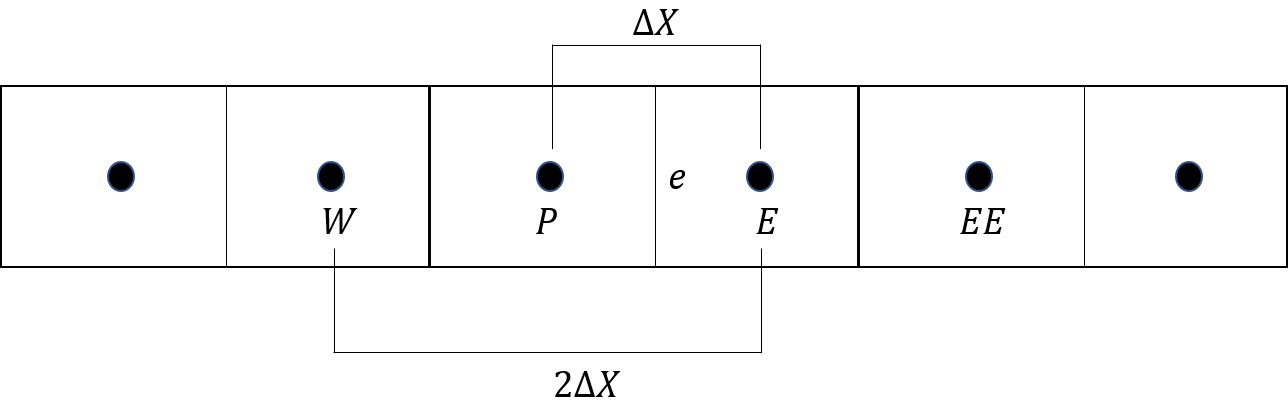
\includegraphics[width=0.6\textwidth]{ch2_litsurvey/Figures/RCinterp_pressureapprox.png}
\caption{Pressure gradient approximation stencils in Rhie Chow interpolation.}
 \label{fig:faceinterp}
\end{figure}

Rhie and Chow~\cite{Rhie1983} introduced an interpolation scheme that allowed the use of pressure correction methods like SIMPLE to be used on collocated grids as well. A dissipation term representing the difference between the two ways of computing the pressure gradient, the $\Delta X$ and the $2\Delta X$ approximations,  is added to the linear interpolation of the velocity at cell faces. 
The velocity at the face, $\overline{u}_e$, at a face $e$ in figure~\ref{fig:faceinterp} is approximated by a linear interpolation as
\begin{equation}
\overline{u}_e = \lambda_P u_P + \lambda_E u_E,
\label{eq:interpvel}
\end{equation}
where $\lambda_P$ and $\lambda_E$ are the weighting factors for nodes $P$ and $E$ respectively. The new interpolation scheme from Rhie and Chow modify the velocity 
at the face as
\begin{equation}
u_e = \overline{u}_e + D_f\left( \left(\frac{\partial p}{\partial x}\right)_e - \overline{\left(\frac{\partial p}{\partial x}\right)}_e \right).
\label{eq:RCorig}
\end{equation}
The term $D_f$ was introduced earlier in equation~\ref{eq:ch2dfeqn}. The $\overline{u}_e$ is the linearly interpolated velocity in equation~\ref{eq:interpvel}. The first term within the brackets is the $\Delta X$ approximation of the pressure gradient and the second term represents the $2\Delta X$ approximation of the pressure gradient. On a uniform $1D$ grid, these derivatives are
\begin{equation}
\left(\frac{\partial p}{\partial x}\right)_e = \frac{p_E - p_P}{\Delta X},
\end{equation}
and
\begin{equation}
\overline{\left(\frac{\partial p}{\partial x}\right)}_e = \frac{1}{2}\left(\frac{p_E - p_P}{\Delta X} + \frac{p_P - p_W}{\Delta X} \right)= \frac{p_E - p_W}{2\Delta X}.
\end{equation}
%This equation will be derived in the next chapter using a different approach.
%Extension of the SIMPLE and other algorithms to collocated grids needs special attention. Momentum interpolation methods to compute the mass flux based on the formulation introduced by Rhie and Chow in~\cite{Rhie1983} is adapted in the current paper to avoid the odd-even decoupling of pressure. 

The new interpolation scheme, commonly referred to as either the Rhie-Chow interpolation or the momentum interpolation, allows the use of the SIMPLE like algorithms on collocated grids. The solution algorithm is very similar to the staggered grid.
\begin{enumerate}
    \item Guess the pressure field $p^{\ast}$.
    \item Solve the momentum equations like equation~\ref{eq:segueqn*} to find the estimated velocities $u_i^{\ast}$.
    \item Use the Rhie-Chow interpolation to compute the velocities at the cell faces.
    \item Find the mass flux at the faces $m_f^{\ast}$ using the cell face velocities.
    \item Assemble the pressure correction equation based on the mass fluxes and the momentum equation.
    \item Solve the pressure correction equation (equation~\ref{eq:pcorrstag2}) to find the pressure and velocity corrections.
    \item Update the pressure and velocity corrections and repeat till convergence.
\end{enumerate}
Other algorithms based on SIMPLE, like SIMPLEC, SIMPLER and PISO can also be used as long as the mass flux imbalance is computed using the new interpolation scheme.
\section{Turbulent flows}
Most flow problems encountered in practical situations, including the flow past wind turbines, are turbulent in nature. Turbulent flows are highly unsteady with the velocity fields fluctuating rapidly in all three dimensions (usually around a mean value). A laminar flow becomes turbulent due to an instability in the flow that gets amplified, either due to external factors or the flow itself, when above a certain critical Reynolds number. Discussing the nature of turbulence is beyond the scope of this thesis and the emphasis of this section is on modeling the effects of turbulence.

Despite the vastly different natures of laminar and turbulent flows, the Navier Stokes equations presented earlier in equations~\ref{eq:continuity}, \ref{eq:xmommentum}, \ref{eq:ymommentum} and \ref{eq:zmommentum} are valid for both situations. However, turbulent flows involve instantaneous fluctuations in three dimensions, rapid mixing and appears random. Unlike laminar flows, there is an additional mechanism for energy transfer which is usually described as an energy cascade. This process describes the transfer of energy from very large eddies (zones of recirculating motion of the fluid) to smaller ones in a cascading process till the size of the eddies are small enough for viscous dissipation to become relevant.

In order to accurately model the energy cascade process, the numerical methods used must resolve all the scales down to the smallest ones, known as the Kolmogrov scales~\cite{Pope2000}. The smallest length scales are characterized by the viscosity of the fluid and for flows at high Reynolds numbers such as the flow around a wind turbine, these scales are extremely small. An accurate representation of eddies at this scale would require enormous computational resources. The computational cost of such simulations can be shown to be proportional to approximately $Re^3$. Such simulations where all the scales of the flow are resolved are known as Direct Numerical Simulations (DNS). Due to the prohibitively expensive computational requirements, DNS can be carried out only for low Reynolds number flows under relatively simple conditions and cannot be applied to problems of practical interest. Thus, approximate approaches that can model the effect of turbulence within reasonable computational costs are sought.

One such approximate solution is to use the Large Eddy Simulations (LES) approach. As the name implies, the larger eddies in a turbulent flow are resolved numerically whereas the statistical nature of the energy cascade process, especially at smaller length scales, is used to model the smaller scales. This lifts some of the more restrictive computational requirements of DNS while still maintaining relatively high accuracy. Despite the still significant computational requirements the use of LES for practical engineering problems is gaining increasing significance. 

However, the most commonly used approach to model turbulent flows is based on the solutions of Reynolds Averaged Navier Stokes equations (RANS). The turbulent flow field is split into a time averaged mean flow and a fluctuating component. The Reynolds averaging process brings the computational requirements for most practical problems to a manageable level while maintaining sufficient accuracy. Combinations of RANS and LES like Detached Eddy Simulation (DES) and Delayed Detached Eddy Simulation (DDES) are becoming increasingly common for practical engineering applications as well. 

The Reynolds averaging and the resulting equations will be described in detail in the following section.
\subsection{Reynolds averaging}\label{ssec:rans}
Any general variable $\phi$ in a turbulent flow is three dimensional and varies with time (figure~\ref{fig:ransfluct}). 
\begin{figure}[h]
\centering
\captionsetup{justification=centering}
 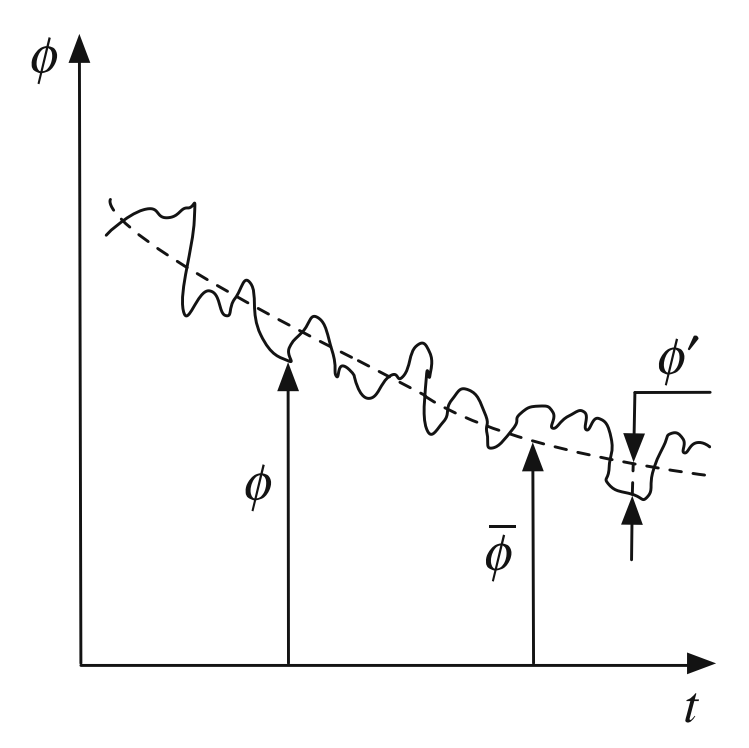
\includegraphics[width=0.45\textwidth]{ch2_litsurvey/Figures/RANSfluctphi.png}
\caption{Fluctuating and mean variable components for a general variable $\phi$~\cite{Moukalled}.}
 \label{fig:ransfluct}
\end{figure}
$\phi$ is assumed to be composed of a mean flow component, $\overline{\phi}$ and a fluctuating component $\phi^{\prime}$ as 
\begin{equation}
\phi(x_i,t) = \overline{\phi}(x_i,t) + \phi^{\prime}(x_i,t).
\end{equation}
The mean flow component can be computed using the Reynolds averaging process~\cite{Moukalled}. Three different approaches are possible
\paragraph{Time averaging}
The mean flow component is found as 
\begin{equation}
\overline{\phi}(x_i,t) = \frac{1}{T}\int_t^{t+T} \phi(x_i,t) dt.
\end{equation}
Here $T$ is the averaging interval which must be large compared to the turbulent fluctuations. This approach is suitable when the mean flow is steady. However, for unsteady mean flows the interval of averaging, $T$, should be chosen such that it is much larger than the time scale of the fluctuations but smaller than the variation of mean flow. This is admittedly difficult and different type of averaging can be used instead.
\paragraph{Ensemble averaging}
The ensemble average is defined as
\begin{equation}
\overline{\phi}(x_i,t) = \frac{1}{N}\sum_N \phi(x_i,t),
\end{equation}
where $N$ is the number of different measurements of $\phi(x_i,t)$. For an accurate ensemble average, the value of $N$ must be as large as possible which is not always practical.
\paragraph{Spatial averaging}
A spatial average represents the average of a quantity over a space interval $\Omega$.
\begin{equation}
\overline{\phi}(x_i,t) = \frac{1}{\Omega}\int_{\Omega} \phi(x_i,t) dx_i.
\end{equation}
This averaging is typically suitable for homogeneous turbulence.
\subsubsection{Properties of Reynolds averaging}
For any two variables $\phi$ and $\psi$ which can be decomposed into a mean flow component ($\overline{\phi}$, $\overline{\psi}$) and a fluctuating component ($\phi^{\prime}$, $\psi^{\prime}$), the following rules apply.
\begin{align}
\overline{\overline{\phi}} = \overline{\phi}, \nonumber\\
\overline{\phi^{\prime}} = 0, \nonumber\\
\overline{\frac{\partial \phi}{\partial x_i}} = \frac{\partial \overline{\phi}}{\partial x_i},\\
\overline{\phi + \psi} = \overline{\phi} + \overline{\psi},\nonumber\\
\overline{\phi \psi^{\prime}} = 0,\nonumber\\
\overline{\phi \psi} = \bar{\phi}\bar{\psi} + \overline{\phi^{\prime} \psi^{\prime}}. \nonumber
\end{align}
\subsection{Incompressible RANS equations}\label{ssec:incomprans}
The Reynolds averaging can be applied to the velocities, $u_i$ and pressure, $p$ to give
\begin{align}
u_i = \overline{u}_i + u_i^{\prime}, \nonumber \\
p = \overline{p} + p^{\prime}.
\end{align}
Substituting these into the continuity equation (equation~\ref{eq:contindx}) and taking the time average gives 
\begin{equation}
\frac{\partial \overline{u}_i}{\partial x_i} = 0.
\label{eq:contindxrans}
\end{equation}
This equation is fundamentally the same as the equation~\ref{eq:contindx}. The divergence condition now applies only to the mean flow components of velocity. Adopting a similar procedure to the momentum equations (equation~\ref{eq:momindx}) and taking the time average gives
\begin{equation}
\frac{\partial \overline{u}_i}{\partial t} + \frac{\partial (\overline{u_iu_j})}{\partial x_j} = -\frac{\partial \overline{p}}{\partial x_i} + \frac{1}{Re}\left( \frac{\partial^2 \overline{u}_i}{\partial x_j\partial x_j} \right).
\label{eq:momindxrans1}
\end{equation}
The unsteady term, pressure gradient term and the viscous diffusion term simplify to a form that is similar to equation~\ref{eq:momindx} but due to the non-linearity of the advective term, special attention is required. Using the property of Reynolds averaging for a product, the advective term can be separated into two components as 
\begin{equation}
\frac{\partial \overline{u}_i}{\partial t} + \frac{\partial (\bar{u_i} \bar{u_j})}{\partial x_j} + \frac{\partial (\overline{u_i^{\prime}u_j^{\prime}})}{\partial x_j} = -\frac{\partial \overline{p}}{\partial x_i} + \frac{1}{Re}\left( \frac{\partial^2 \overline{u}_i}{\partial x_j\partial x_j} \right).
\label{eq:momindxrans2}
\end{equation}
The additional term involving the product of the fluctuating velocity components is unknown and thus the incompressible RANS equations are not closed. This additional term is known as the Reynolds stress tensor and equation~\ref{eq:momindxrans2} is usually written as 
\begin{equation}
\frac{\partial \overline{u}_i}{\partial t} + \frac{\partial (\bar{u_i} \bar{u_j})}{\partial x_j} = -\frac{\partial \overline{p}}{\partial x_i} + \frac{1}{Re}\left( \frac{\partial^2 \overline{u}_i}{\partial x_j\partial x_j} \right) - \frac{\partial (\overline{u_i^{\prime}u_j^{\prime}})}{\partial x_j}.
\label{eq:momindxrans3}
\end{equation}

For the commonly used eddy viscosity models, the Reynolds stress tensor is modeled based on the Boussinesq hypothesis~\cite{Pope2000}, where an analogy between the viscous stresses and Reynolds stresses are made. For a Newtonian fluid, the viscous stresses are a linear function of the mean velocity gradients (mean rate of strain) with the constant of proportionality being the dynamic viscosity of the fluid
\begin{equation}
\tau = \mu \left[\left(\frac{\partial u_i}{\partial x_j} + \frac{\partial u_j}{\partial x_i}\right) - \frac{2}{3}\delta_{ij}\frac{\partial u_i}{\partial x_i}\right].
\end{equation}
Similarly, the Reynolds stresses are assumed to be a linear function of the mean velocity gradients and the proportionality constant being the newly defined turbulent eddy viscosity, $\mu_t$, as
\begin{equation}
\tau^R = - \frac{\partial (\overline{u_i^{\prime}u_j^{\prime}})}{\partial x_j} = \mu_t \left(\frac{\partial u_i}{\partial x_j} + \frac{\partial u_j}{\partial x_i}\right) - \frac{2}{3}\delta_{ij}\left(\rho k + \mu_t\frac{\partial u_i}{\partial x_i}\right).
\end{equation}
Here $\rho$ is the density and $k$ is known as the turbulent kinetic energy defined as
\begin{equation}
k = \frac{1}{2}\overline{u_i^{\prime} u_i^{\prime}}.
\end{equation}
For incompressible flows the divergence of the mean flow velocity is zero and the turbulent kinetic energy term is absorbed into the pressure or simply neglected. This leaves only the turbulent eddy viscosity as the new unknown.

\subsubsection{Turbulent eddy viscosity models}
Using the Boussinesq hypothesis, instead of the unknown Reynolds stress tensor now only a single unknown turbulent eddy viscosity remains. This eddy viscosity can be expressed as a function of a velocity scale ($V$) and a length scale ($l$) based on dimensional analysis as
\begin{equation}
\mu_t = C_{\mu}\rho l V,
\end{equation}
where $C_{\mu}$ is a dimensionless constant. Different eddy viscosity models have been proposed to find these velocity and length scales. The most popular class of these models are the one and two equation turbulence models. An example of a one equation turbulence model is the Spalart-Allmaras model~\cite{spalart1992one} where a scalar transport equation similar to equation~\ref{eq:genphi} is written for a new variable $\tilde{\nu}$. The most common examples of two equation models are the $k$-$\omega$ model from Wilcox~\cite{wilcox1988komega,wilcox2008komega}, the $k$-$\epsilon$ model from Jones and Launder~\cite{launder1974kepsilon,jones1972kepsilon} and the $k$-$\omega$ SST model from Menter~\cite{menter1994two}.

Presently, the one equation SA turbulence model and the two equation $k$-$\omega$ SST turbulence model are available in SU2. 

\subsection{Solution procedure}
Previously, the solution procedure for the incompressible Navier Stokes equations on a collocated grid was described in section~\ref{ssec:collocated}. By solving the turbulence equations in a segregated manner with the flow equations, the solution algorithm does not change significantly. The algorithm for solving the incompressible RANS equations is 
\begin{enumerate}
    \item Guess the pressure field $p^{\ast}$.
    \item Solve the momentum equations like equation~\ref{eq:segueqn*} to find the estimated velocities $u_i^{\ast}$.
    \item Use the Rhie-Chow interpolation to compute the velocities at the cell faces.
    \item Find the mass flux at the faces $m_f^{\ast}$ using the cell face velocities.
    \item Assemble the pressure correction equation based on the mass fluxes and the momentum equation.
    \item Solve the pressure correction equation (equation~\ref{eq:pcorrstag2}) to find the pressure and velocity corrections.
    \item Update the pressure and velocity corrections and update the mean flow gradients.
    \item Solve the turbulence model equations to find the eddy viscosity $\mu_t$ to be used in the next iteration.
    \item Repeat till convergence.
\end{enumerate}

More details about the models and their implementation will be presented in the next chapter.

\bibliographystyle{dissertation}
\bibliography{ch2_litsurvey/su2references}
%\references{su2references}
\chapter[Pressure based incompressible solver in SU2]{Pressure based incompressible solver in SU2}
\label{ch:ch3su2eqn}

%% The following annotation is customary for chapter which have already been
%% published as a paper.
%\blfootnote{footnote}

%% It is only necessary to list the authors if multiple people contributed
%% significantly to the chapter.
\begin{abstract}
The previous chapter described the incompressible flow equations and the approach to solve them numerically. This chapter describes the implementation of those numerical methods in SU2. The implementation details of the different boundary conditions, under-relaxation techniques, turbulence models will also be discussed.
\end{abstract}
%
%%%%%%%%%  
%In this chapter, the governing equations of the new solver are described along with spatial and time integration methods.

%%%%%%%%%%%%%%%%%%%%%%%%%%%%%%%%%%%%%%%%%%%%%%%%%%%%
%%%%%%%%%%%%%%%%%%%%%%%%%%%%%%
%\section{More sections}\label{sec:asymptotic}
%\section{Model equations}\label{sec:goveqn}
The general structure of the partial differential equation (PDE) solved in SU2 is of the form~\cite{SU22014} 
\begin{equation}
\frac{\partial U}{\partial t}  + \frac{\partial F^c}{\partial x_i}-\frac{\partial F^v}{\partial x_i}=Q \quad \text{in} \quad \Omega, \quad t>0,
\label{eq:generic}
\end{equation}
%\nomenclature[A]{$U$}{Solution vector}
where $U$ is the vector of state variables, $F_i^c$ are the convective fluxes, $F^v_i$ are the viscous fluxes and $Q$ is a source term. In the pressure based solver the momentum equations and the pressure correction equation are solved sequentially. The momentum equation remains in the same form as equation~\ref{eq:generic} and the pressure correction equation is derived based on a combination of the momentum and continuity equations as described in the previous chapter. 
\section{Momentum equation}\label{sec:momeq}
For the momentum equations, the terms in equation~\ref{eq:generic} are 
\begin{align}
    U_i = \rho u_i,\quad
    F^c_i = 
           \rho u_i u_j,\quad
    F^v_i = 
           \tau_{ij},\quad
    Q = -\frac{\partial p}{\partial x_i}
\end{align}
%\nomenclature[A]{$\Omega$}{Domain of the problem}
%\nomenclature[A]{$|\Omega|$}{Volume of the domain under consideration}
where $u_i$ are the components of the velocity vector, $\rho$ is the density, $p$ is the gauge pressure ($p - p_{ref}$, where $p_{ref}$ is a reference pressure) and the viscous stresses for incompressible flow are 
\begin{equation}
\tau_{ij}=\mu_{tot}\left(\frac{\partial u_i}{\partial x_j} + \frac{\partial u_j}{\partial x_i} \right).
\label{eq:viscstress}
\end{equation} 
The total viscosity coefficient, $\mu_{tot}$ is the sum of the dynamic viscosity $\mu_{dyn}$ and turbulent eddy viscosity $\mu_{tur}$, which is computed via a turbulence model. 
%The Spalart-Allmara(S-A) and the Mean Shear Stress Transport(SST) turbulence models can be used to compute $\mu_{tur}$.
%\nomenclature[S]{$\rho$}{Density}%
%\nomenclature[S]{$\mu_{dyn}$}{Dynamic viscosity}%
%\nomenclature[S]{$\mu_{tur}$}{Turbulent viscosity}%
%\nomenclature[S]{$\mu_{tot}$}{Total viscosity}%

\subsection{Spatial discretization}\label{ssec:spdisc}

The spatial discretization of equation~\ref{eq:generic} is performed on an edge based dual grid using the finite volume approach~\cite{Moukalled, Ferziger2002, BLAZEK}. The discretization procedure follows along the same lines as described in section~\ref{sec:ch2disceqnphi}. The control volumes are constructed using a median-dual (vertex-based) scheme~\cite{barth1992aspects, SU22014}. The control volume faces are created exactly midway between the adjacent nodes. An illustration of the construction of the dual cell is shown in figure~\ref{fig:dualcell}. The solution is computed at the nodes shown at the intersection  of the solid grid lines. 
%Control volumes are constructed around each of these nodes where the fluxes are evaluated. 
\begin{figure}[h]
\centering
\captionsetup{justification=centering}
 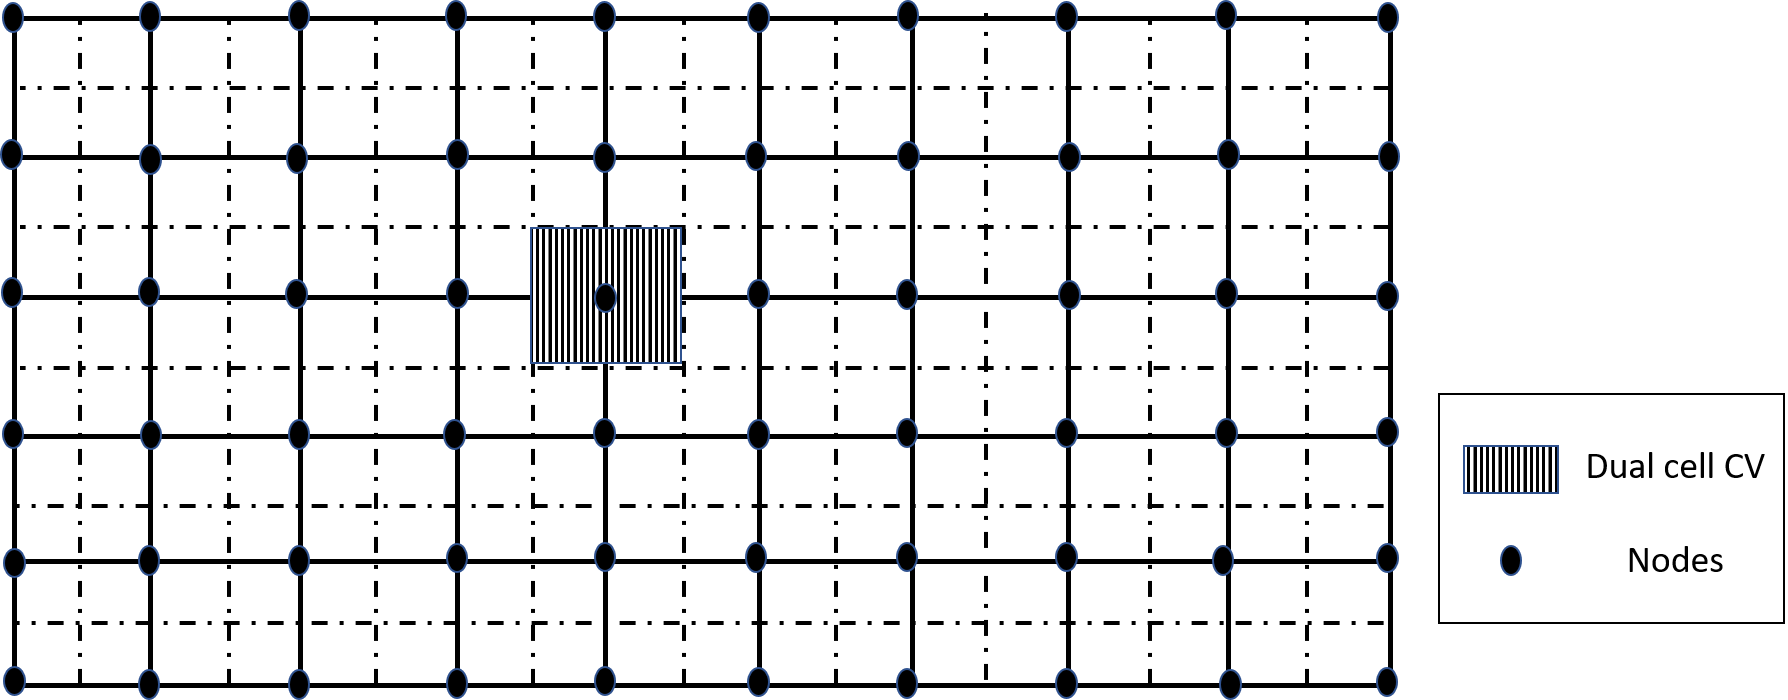
\includegraphics[width=0.65\textwidth]{ch3_su2eqn/figures/dual_cell_nodes.png}
\caption{Dual cell structure on a $2D$ domain.}
 \label{fig:dualcell}
\end{figure}

\noindent Integrating equation~\ref{eq:generic} over one control volume (CV) with a volume of $\Omega$ gives,
\begin{equation}
\int_{\Omega}\frac{\partial U}{\partial t}d\Omega + \int_{\Omega}\frac{\partial}{\partial x_i} (F^c_i-F^v_i)d\Omega = -\int_{\Omega}\frac{\partial P}{\partial x_i} d\Omega.
\end{equation}
Using the divergence theorem on the convective and viscous flux terms results in
\begin{equation*}
\int_{\Omega}\frac{\partial U}{\partial t}d\Omega+\int_{\partial\Omega}(F^c_i-F^v_i)n_i dS=-\int_{\Omega} \frac{\partial P}{\partial x_i}d\Omega,
\end{equation*}
\begin{equation}
\int_{\Omega}\frac{\partial U}{\partial t}d\Omega +R(U)=-F^{p},
\label{eq:fvmeqn}
\end{equation}
%\nomenclature[U]{$c$}{Convective fluxes}%
%\nomenclature[U]{$p$}{Pressure contribution}%
%\nomenclature[U]{$v$}{Viscous fluxes}%
%\nomenclature[U]{$\ast$}{Estimate}%
%\nomenclature[U]{$\prime$}{Correction}%
where $R(U)$ is the residual vector consisting of the discretized convective and viscous fluxes, $F^c$ and $F^v$. The pressure gradient is treated as a source term and its discretized form, $F^p$, is found using the mid point integration rule in the CV and is given by
\begin{equation}
\int_{\Omega} \frac{\partial P}{\partial x_i}d\Omega  \approx |\Omega|\frac{\partial P}{\partial x_i} = F^{p}.
\label{eq:pressapprox}
\end{equation}

\paragraph{Discretization of the viscous term}
For the dual cell, the surface integral of the viscous fluxes can be transformed into a summation along the CV faces.
\begin{equation}
\int_{\partial\Omega}F^{v}_in_i dS \approx \sum_{\partial \Omega} \tau_{ij} n_i \Delta S.
\end{equation}
A central scheme is used to find $\tau_{ij}$ at the face $f$.  For the nodes $P$ and $F$ separated across the face $f$ (figure~\ref{fig:nonorthonodes}),
\begin{equation}
\tau_{ij}|_f = \frac{1}{2}\left(\tau_{ij}|_P + \tau_{ij}|_F\right).
\end{equation}
A correction is applied to account for the non orthogonality of the mesh. For a general variable $\phi$ the derivative in the normal direction is evaluated as
%\begin{equation}
%    \nabla \phi \cdot \vec{n} = \frac{\phi_j - \phi_i}{|x_j - x_i|}\alpha_f + \frac{1}{2}(\nabla \phi|_i + \nabla \phi|_j)\cdot(\vec{n} - \alpha_f \vec{s}),
%    \label{eq:gradrel}
%\end{equation}{}
\begin{equation}
   \left(\frac{\partial \phi}{\partial n}\right)_f = \frac{\phi_F - \phi_P}{d_{PF}} + \frac{1}{2}\left(\frac{\partial \phi}{\partial x_i}\bigg|_P +\frac{\partial \phi}{\partial x_i}\bigg|_F\right)(n_i - \alpha_f s_i),
    \label{eq:gradrel}
\end{equation}{}
where $n_i$ is the face normal, $s_i$ is the normalized vector connecting the cell centers $P$ and $F$ across the face $f$, $d_{PF}$ is the distance between the nodes $P$ and $F$ and $\alpha_f = s_i n_i$. 
\begin{figure}[h]
\centering
\captionsetup{justification=centering}
 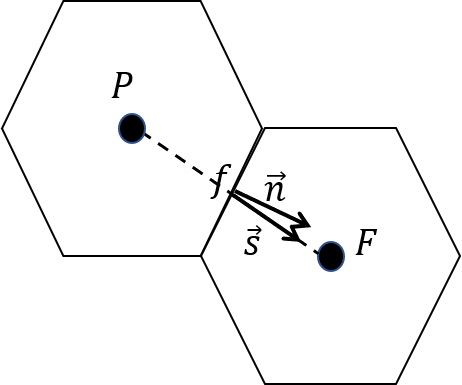
\includegraphics[width=0.3\textwidth]{ch3_su2eqn/figures/noncollinearij.png}
\caption{Nodes $P$ and $F$.}
 \label{fig:nonorthonodes}
\end{figure} 
No correction is applied for the boundary elements. The gradients at the cell centers $P$ and $F$ can be computed using either the Green-Gauss or the Least Squares method~\cite{Moukalled}.

\paragraph{Discretization of the convective term }
The convective fluxes are discretized using a standard upwind scheme and second order accuracy is achieved via reconstruction of variables at the cell faces as described in section~\ref{sec:ch2disceqnphi}. The discretized form of the convective term of the momentum equations is
\begin{equation}
\int_{\partial\Omega}F^{c}_i n_i dS \approx \sum_{\partial \Omega} (\rho u_i n_i)u_j \Delta S = \sum_{\partial \Omega}\dot{m}_f u_j,
\end{equation}
where $\dot{m}_f$ is the mass flux across each face $f$ along the boundary ($\partial\Omega$) of the control volume, $n_i$ is the unit outward normal vector of face $f$ and $u_j$ are the velocity components. 
\begin{figure}[h!]
    \centering
    \captionsetup{justification=centering}
    \begin{subfigure}[b]{0.48\textwidth}
    \centering
    \captionsetup{justification=centering}
        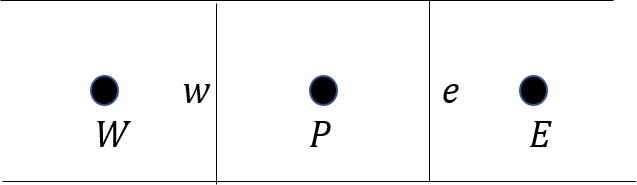
\includegraphics[width=0.75\textwidth]{ch3_su2eqn/figures/1dcv.png}
        \caption{$1D$ control volume around a node $P$.}
        \label{fig:1dd}
    \end{subfigure}
    \begin{subfigure}[b]{0.48\textwidth}
    \captionsetup{justification=centering}
        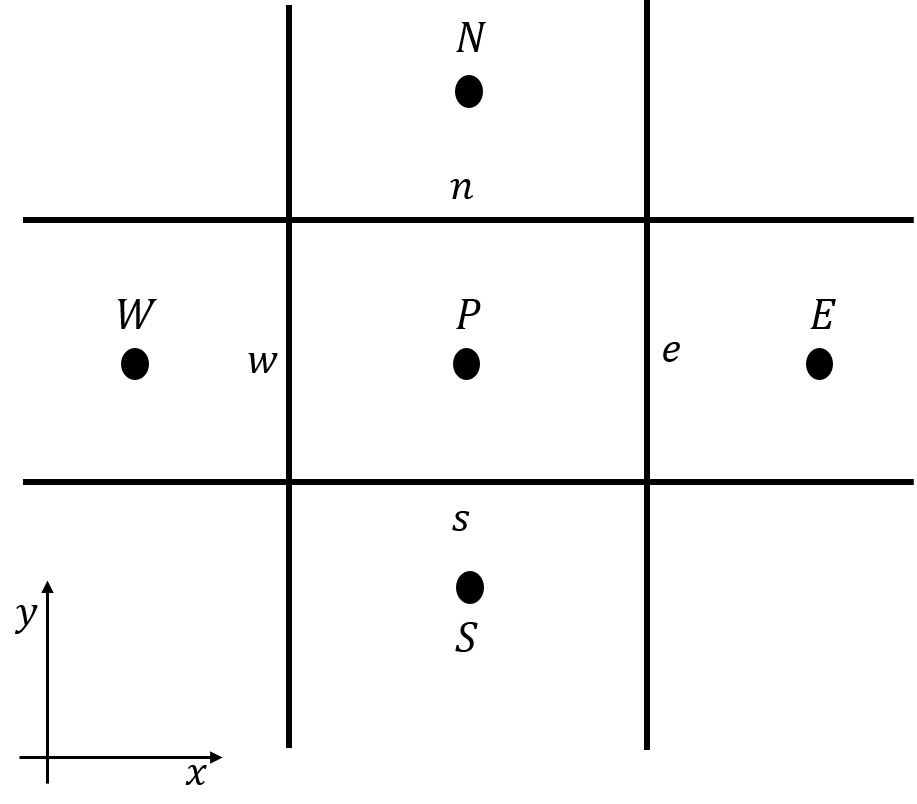
\includegraphics[width=0.75\textwidth]{ch2_litsurvey/Figures/2ddomainwaxisneigh.png}
        \caption{$2D$ control volume around a node $P$.}
        \label{fig:2dd}
    \end{subfigure}
    \caption{Control volume around a node $P$ in (a) $1D$ and (b) $2D$.}
\end{figure}
For instance, on a $1D$ domain (see figure~\ref{fig:1dd}) the discretized form of the convective term is
\begin{equation}
\sum_{\partial \Omega}\dot{m}_f u_j = (\dot{m}u)_e + (\dot{m}u)_w.
\end{equation}
and on a $2$D domain (see figure~\ref{fig:2dd}) the discretized form of the convective term is
\begin{equation}
\sum_{\partial \Omega}\dot{m}_f u_j = (\dot{m}u_j)_e + (\dot{m}u_j)_w + (\dot{m}u_j)_n + (\dot{m}u_j)_s.
\end{equation}
Here $e$,$w$,$n$ and $s$ represent the east, west, north and south face of the CV respectively and $u$ and $v$ are the horizontal and vertical components of velocity. The velocity at the face is reconstructed from the upwind direction which is determined based on the direction of mass flux at each face. For example, for the face $e$, let the neighboring node be $E$. The direction is found as follows. First compute the mass flux across the face, $\dot{m}_e$
\begin{equation*}
\dot{m}_e = \frac{1}{2}\rho (u_{i,P} + u_{i,E})n_i.
\end{equation*}
Define two temporary quantities,
\begin{align*}
\dot{m}_P = \frac{1}{2}(\dot{m}_e + |\dot{m}_e|), \\
\dot{m}_E = \frac{1}{2}(\dot{m}_e - |\dot{m}_e|).
\end{align*}
The upwind direction can then be found as,
\begin{align*}
dir_P = \left\lfloor \frac{\dot{m}_P}{|\dot{m}_e|}\right\rceil, \\
dir_E = \left\lfloor \frac{\dot{m}_E}{|\dot{m}_e|}\right\rceil.
\end{align*}
\noindent Here $ \left\lfloor\right\rceil$ represent rounding to the nearest integer. 
%Clearly, if the flow is from $P$ towards $E$, $\dot{m}_e$ is positive and $dir_P$ becomes $1$ while $dir_E$ becomes zero and vice versa. 
Finally, the velocity at the face $e$ can be found as
\begin{equation}
u_{j,e} = (dir_P) u_{j,P} + (dir_E) u_{j,E}.
\end{equation}
This gives a first order upwind approximation which as seen in section~\ref{sec:ch2disceqnphi} is not very accurate. The velocities at the nodes, $u_{i,P}$ and $u_{i,E}$ can be reconstructed at the face $e$ to obtain a second order upwind scheme. This option is available to the user. SU2 also has different slope limiters to maintain monotonicity of the upwind scheme. The effect of using a slope limiter was also shown in section~\ref{sec:ch2disceqnphi}.


\subsection{Time integration: Steady state problems}\label{sssec:timediscr}
Steady state problems are solved using a pseudo unsteady method. Instead of using an iterative algorithm the solution is marched in time. For steady state problems, the time integration is done using an implicit Euler scheme. Let the solution at a node $P$ at time $t^{n+1}$ be $U_i^{n+1}$. Using an implicit Euler scheme on equation~\ref{eq:fvmeqn},
\begin{equation}
\int_{\Omega}\frac{\partial U^{n+1}_P}{\partial t}d\Omega +R_P(U^{n+1}) + F^{p,n}_P \approx 
\frac{\partial U^{n+1}_P}{\partial t} |\Omega|_P + R_P(U^{n+1}) + F^{p,n}_P.
\end{equation}

A backward Euler time integration scheme is used to discretize the time derivative. The final discretized equation using the procedure outlined in section~\ref{sec:ch2disceqnphi}, can be written as
%Using the backward Euler implicit scheme on the time derivative,
%\begin{equation}
%\frac{U^{n+1}_P - U^n_P}{\Delta t^n_P}|\Omega| +R_P(U^{n+1})  = -F^{p,n}_P.
%\end{equation}
%Since the residual at time $t^{n+1}$ is also unknown, it is linearized about time $t^n$
%\begin{equation}
%R_P(U^{n+1})  = R_P(U^n) + \sum_{\mathcal{N}(P)}\frac{\partial R_P(U^n)}{\partial U_{\mathcal{N}(P)}}\Delta U^n_P + \mathcal{O}(\Delta t^2).
%\end{equation}
%This approximation is valid only when solving for a steady state solution. Thus, the final system of equations can be written as
%\begin{equation*}
%    \left( \frac{|\Omega|}{\Delta t_P^n}\delta_{ij}+\frac{\partial R_{P}(U^n_i)}{\partial U_{j}} \right) \Delta U_{j}^n=-R_P(U^n_j)-F_{P}^{p,n},
%\end{equation*}
%or
\begin{equation}
\boldsymbol{A}^n \Delta\mathbf{U}^n=\mathbf{B}^n.
\label{eq:momeqfinal}
\end{equation}
$\boldsymbol{A}^n$ is the matrix of coefficients at a time level $t^n$ like $\mathbf{a}_{P,i}^n$, 
\begin{align*}
\boldsymbol{A}^n = \begin{bmatrix}
\vdots & & \vdots  & & \vdots \\
 & \ddots & & \ddots  \\
\dots & & \mathbf{a}_{P,i}^n & & \dots\\
 & \ddots & & \ddots  \\
\vdots & & \vdots  & &\vdots
\end{bmatrix},
\end{align*}
$\Delta\mathbf{U}^n$ is the vector containing the update to the solution at all the nodes at a time level $t^n$ and $\mathbf{B}^n$ is the vector containing the residual and pressure contributions from all the nodes,
\begin{align*}
\Delta\mathbf{U}^n = \begin{pmatrix}
\vdots\\
\Delta U_{P,i}^n \\
\vdots
\end{pmatrix},
\qquad
\mathbf{B}^n = \begin{pmatrix}
\vdots \\
-R(U^{n}_{P,i})-F^{p}_i\\
\vdots
\end{pmatrix},
\quad
i=1,2,3.
\end{align*}
%Here  denotes the component of velocity.


%\begin{equation*}
%\boldsymbol{A}_{ij} = \left(\frac{|\Omega|}{\Delta t}\delta_{ij}+\frac{\partial R_{i}}{\partial U_{j}}\right),
%\end{equation*} 
%is the coefficient matrix and $\Delta U^n = U^{n+1}-U^n$ is the update to the solution at time $t^n$. 

A local time stepping scheme is used to accelerate the convergence as each cell advances at a suitable local time step. This local time step is calculated as the minimum of the time steps obtained from convective and viscous terms. The steady solution is obtained faster if larger time steps are used. Also, since time accuracy is not desired when running steady state simulations, the largest possible time step that does not cause the solution to diverge is chosen.
\begin{equation}
\Delta t = min(\Delta t_{conv}, \Delta t_{visc}),
\end{equation}
\begin{equation}
\Delta t_{conv} = CFL\frac{|\Omega|}{\lambda_{conv}}, \qquad
\Delta t_{visc} = CFL\frac{|\Omega|^2}{\lambda_{visc}}.
\end{equation}
where $CFL$ is a user defined value and
\begin{equation}
\lambda_{conv} = \sum_{f}|u_{i,f} n_{i,f}|\Delta S,
\end{equation}
is the sum of the magnitude of the projected face velocity across all the faces of the control volume surrounding a node and 
\begin{equation}
\lambda_{visc} = \sum_{f}C\frac{\mu_{tot}}{\rho}\Delta S^2,
\end{equation}
is the viscous spectral radius~\cite{SU22014}. Here $C$ is a constant and is set to $C=0.25$. In order to avoid the possibility of division by zero, the convective term is changed to 
\begin{equation}
\lambda_{conv} = \sum_{f}|(u_f + u_{ref}) \cdot \vec{n}_f|\Delta S,
\end{equation}
where $u_{ref}$ is a reference velocity. 
%Since the aim of the time integration is to reach a steady state solution, time accuracy is not important and the time step sizes are chosen to ensure fast convergence without causing divergence.
\subsubsection{SIMPLE}
As explained in chapter 2, the SIMPLE algorithm is used to calculate the velocity and pressure in an iterative manner. However, since a pseudo time stepping scheme is used for steady state problems, the time steps take the place of iterations. Thus starting from a time step $t^n$, the velocities and pressure at the next time step $t^{n+1}$ is found as follows. The momentum equations are first solved using the pressure, $p^{n}$ at time $t^n$ to give an estimated velocity field, $u_{i}^{\ast}$. 
\begin{equation}
u_{i}^{\ast} = u_{i}^{n} + \Delta u_{i},
\end{equation}
where $\Delta u_{i}$ is found from the solution of equation~\ref{eq:momeqfinal} as $\Delta u_{i} = \frac{\Delta U_{i}}{\rho}$. 
The estimated velocities and pressure are then corrected based on velocity and pressure corrections.
\begin{align}
u_i^{n+1} = u_i^{\ast} + u_i^{\prime},\label{eq:vcorr}\\
p^{n+1} = p^n + p^{\prime}.
\label{eq:pcorr}
\end{align}
The pressure and velocity corrections are found by solving a Poisson equation. The Poisson equation is derived based on the continuity equation and the momentum equations. This procedure is described in the following section.

\section{Continuity equation}
So far, only the momentum equations have been used to find an estimate of the velocity based on the existing pressure field. In order to correct the velocity estimations and the pressure, the continuity equation must be used to close the system of equations. However, since the continuity equation does not contain any pressure terms a new equation for pressure has to be obtained. This new equation for pressure is derived starting from the discrete form of the continuity equation for an incompressible flow 
\begin{equation}
    \int_{\Omega}\frac{\partial \rho u_i}{\partial x_i} \approx \sum_{\partial \Omega}\rho u_{f,i} n_{f,i}\Delta S = \sum_{\partial \Omega}\dot{m}_{f} = 0 ,
    \label{eq:mfeqn}
\end{equation}
where $u_f$ is the velocity at a face $f$, $\rho$ is the fluid density and $n_i$ is the unit outward face normal and $\Delta S$ is the area. Using a linear interpolation to find this face velocity on collocated grids leads to the well known checkerboard problem in the pressure as seen in the previous chapter and thus momentum interpolation techniques are used. Previously, the momentum interpolation proposed by Rhie and Chow~\cite{Rhie1983} was given with only a conceptual explanation. The same interpolation can also be seen as equivalent to writing a pseudo momentum equation at every face with the coefficients linearly interpolated from the momentum equations of the neighboring nodes~\cite{Moukalled}. Thus, in a sense the momentum interpolation mimics the staggered grid approach on collocated grids. This can also be interpreted as adding a third order derivative of the pressure to stabilize the oscillations in the pressure field~\cite{Ferziger2002}.
%\nomenclature[A]{$\dot{m}_f$}{Mass flux across a face $f$}

\subsection{Momentum interpolation of velocities}
In this section, equation~\ref{eq:RCorig} is derived using an alternative approach following Moukalled et al.~\cite{Moukalled} but adapted to the solution procedure used in SU2. The momentum equation in the $x$ direction for a node $P$ (see figure~\ref{fig:1dd}) can be written as
\begin{equation*}
\mathbf{a}_{P}^{n,u}\Delta u_{P}^n+\sum_{C \in \mathcal{N}(P)} \mathbf{a}_{C,u}^{n,u}\Delta u_{C}^n=-R(u_{P}^{n})- |\Omega|\left(\frac{\partial p^n}{\partial x}\right)_{P} 
\end{equation*}
where $\mathbf{a}_{P}^{n,u}$ is the coefficient of $u$, the velocity along the $x$ direction at the node $P$, $\mathbf{a}_{C}^{n,u}$ is the coefficient of the same velocity component at a node $C$ which is a neighbor of node $P$ ($C \in \mathcal{N}(P)$), $R(u_{P}^{n})$ is the residual computed explicitly and $|\Omega|$ is the volume of the control volume around node $P$. Here ${\mathcal{N}(P)}$ represents the neighbors the node $P$. Since the density is assumed to be constant, it is absorbed in to the coefficients $\mathbf{a}_{P}^{n,u}$ and $\mathbf{a}_{C}^{n,u}$.

The estimate of the velocity at a node $P$ for time level $n+1$ can be written as 
\begin{equation}
u_{P}^{\ast}=u_{P}^{n}+\Delta u_{P}^n=u_{P}^{n}-\frac{1}{\mathbf{a}_{P}^{n,u}}\left(R(u^{n}_{P})+\sum_{C \in \mathcal{N}(P)} \mathbf{a}_{C,u}^n\Delta u_{C}^n+|\Omega|\left(\frac{\partial p^n}{\partial x}\right)_{P} \right),
\end{equation}
Let $H(u^n_P)$ denote  
\begin{equation*}
H(u^n_P)=\frac{1}{\mathbf{a}_{P}^{n,u}}\left(R(u^{n}_{P})+\sum_{C \in \mathcal{N}(P)} \mathbf{a}_{C,u}^n\Delta u_{C}^n\right).
\end{equation*}
The velocity estimates at a node $P$ at time level $t^{n+1}$ can now be re-written as
\begin{equation}
u_{P}^{\ast} = u_{P}^n - H(u^n_P) - \frac{|\Omega|}{\mathbf{a}_{P}^{n,u}}\left(\frac{\partial p^n}{\partial x}\right)_{P}.
\label{eq:velatP}
\end{equation}
Since the pressure gradient used so far is only an estimate, the velocities found using this formula are also an estimate and do not yet satisfy the continuity equation and are thus denoted by $u^{\ast}_i$. 

%\begin{figure}[h]
%\centering
%\captionsetup{justification=centering}
% 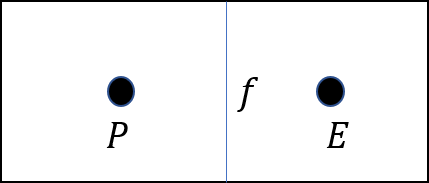
\includegraphics[width=0.2\textwidth]{ch3_su2eqn/figures/PEf_RCinterp.png}
%\caption{Nodes $P$ and $E$ across a face $f$.}
% \label{fig:pefrcinterp}
%\end{figure}
%\noindent
Consider another node $E$, which is a neighbor of node $P$ across the face $e$ in figure~\ref{fig:1dd}. The velocities at node $E$ can be written similar to equation~\ref{eq:velatP} as
\begin{equation}
u_{E}^{\ast} = u_{E}^n - H(u^n_E) -  \frac{|\Omega|}{\mathbf{a}_{E}^{n,u}}\left(\frac{\partial p^n}{\partial x}\right)_{E} .
\label{eq:velatE}
\end{equation}
Since the momentum interpolation technique mimics the staggered approach where velocities are stored on cell faces, hypothetically at the face $e$ between $P$ and $E$, the velocities, $u_{f,i}$ can be written as,
\begin{equation}
u_{e}^{\ast} = u_{e}^n - H(u^n_e) -  \frac{|\Omega|}{\mathbf{a}_{e}^{n,u}}\left(\frac{\partial p^n}{\partial x}\right)_{e} .
\label{eq:velatf}
\end{equation}

\noindent
The coefficients for the hypothetical momentum equation at the face $f$ are assumed to  be interpolated linearly from the neighboring nodes $P$ and $E$ as
\begin{equation}
H(u^n_e)=(\lambda_P H(u^n_P)+\lambda_E H(u^n_E)),
\label{eq:Beqn}
\end{equation}{}
\noindent where $\lambda_P$ and $\lambda_E$ are the weighting factors for the interpolation. Since a median dual grid is used for discretization, the faces are always midway between the two nodes. Thus, $\lambda_P = \lambda_E = 1/2$. Substituting for $H_{f,i}^n$, $H_{P,i}^n$ and $H_{E,i}^n$ in equation~\ref{eq:Beqn} from equations~\ref{eq:velatf}, \ref{eq:velatP} and \ref{eq:velatE} respectively and expanding the pressure source term from equation~\ref{eq:pressapprox}, the velocity at a face $f$ after the momentum equation is
\begin{align}
u_{e}^{\ast} &= u_{e}^n - \left(\lambda_P u_{P}^n + \lambda_E u_{E}^n \right) +\left(\lambda_P u_{P}^{\ast} + \lambda_E u_{E}^{\ast}\right) - \frac{|\Omega|_{f}}{\mathbf{a}_{e}^n}\left(\frac{\partial p^n}{\partial x}\right)_e \nonumber \\&+ \left(\lambda_P\frac{|\Omega|_{P}}{\mathbf{a}_{P}^n}\left(\frac{\partial p^n}{\partial x}\right)_{P} + \lambda_E\frac{|\Omega|_{E}}{\mathbf{a}_{E}^n}\left(\frac{\partial p^n}{\partial x}\right)_{E}\right) 
\label{eq:velatf*st1}
\end{align}
Let $\boldsymbol{D}_{P}^{n,u}$ denote
\begin{equation}
\boldsymbol{D}_{P}^{n,u} = \frac{|\Omega|}{\mathbf{a}_{P}^{n,u}}.
\label{eq:Dfeqn}
\end{equation}
Using the new notation, equation~\ref{eq:velatf*st1} can be written as
\begin{align}
u_{e}^{\ast} &= u_{e}^n - \left(\lambda_P u_{P}^n + \lambda_E u_{E}^n\right) +\left(\lambda_P u_{P}^{\ast} + \lambda_E u_{E}^{\ast}\right) - \boldsymbol{D}_{e}^{n,u}\left(\frac{\partial p^n}{\partial x_i}\right)_e \nonumber \\&+ \left(\lambda_P\boldsymbol{D}_{P}^{n,u}\left(\frac{\partial p^n}{\partial x}\right)_{P} + \lambda_E\boldsymbol{D}_{E}^{n,u}\left(\frac{\partial p^n}{\partial x}\right)_{E}\right).
\label{eq:velatf*st2}
\end{align}
The linear interpolation of the pressure gradient terms from nodes $P$ and $E$ are approximated as
\begin{align}
 \left(\lambda_P\boldsymbol{D}_{P}^{n,u}\left(\frac{\partial p^n}{\partial x}\right)_P + \lambda_E\boldsymbol{D}_{E}^{n,u}\left(\frac{\partial p^n}{\partial x}\right)_E\right) &=\overline{\boldsymbol{D}}_{e}^{n,u}\overline{\left(\frac{\partial p^n}{\partial x}\right)_e}.  \label{eq:pbarassump}
\end{align}
The terms under the over bar are linearly interpolated. This approximation is second order accurate~\cite{Moukalled}. Also the coefficient of the pressure gradient at the face is assumed to be the same as the linearly interpolated value i.e. 
\begin{align*}
\boldsymbol{D}_{e}^{n,u} &= \overline{\boldsymbol{D}}_{e}^{n,u}.
\end{align*}
Additionally, the linearly interpolated terms are written with an over bar as follows
\begin{align*}
(\lambda_P u_{P}^{\ast} + \lambda_E u_{E}^{\ast}) &= \overline{u}_{e}^{\ast}, \\
(\lambda_P u_{P}^{n} + \lambda_E u_{E}^{n}) &= \overline{u}_{e}^{n}.
\end{align*}
Equation~\ref{eq:velatf*st1} can now be written as
\begin{equation}
u_{e}^{\ast}=\overline{u}_{e}^{\ast}-\overline{\boldsymbol{D}}_{e}^{n,u}\left(\left(\frac{\partial p^n}{\partial x}\right)_{e}-\overline{\left(\frac{\partial p^n}{\partial x}\right)_{e}}\right) + \left(u_{e}^n - \overline{u}_{e}^n\right).
\label{eq:uvelatf*}
\end{equation}
Analogously, the $y$ and $z$ components of the velocity can be written as
\begin{align}
v_{e}^{\ast}&=\overline{v}_{e}^{\ast}-\overline{\boldsymbol{D}}_{e}^{n,v}\left(\left(\frac{\partial p^n}{\partial y}\right)_{e}-\overline{\left(\frac{\partial p^n}{\partial y}\right)_{e}}\right) + \left(v_{e}^n - \overline{v}_{e}^n\right).
\label{eq:vvelatf*}\\
w_{e}^{\ast}&=\overline{w}_{e}^{\ast}-\overline{\boldsymbol{D}}_{e}^{n,w}\left(\left(\frac{\partial p^n}{\partial z}\right)_{e}-\overline{\left(\frac{\partial p^n}{\partial z}\right)_{e}}\right) + \left(w_{e}^n - \overline{w}_{e}^n\right).
\label{eq:wvelatf*}
\end{align}

\subsubsection{Effect of pseudo time stepping}
Recall the expression for the face velocity based on the momentum interpolation in Eq. \ref{eq:uvelatf*}, 
\begin{equation*}
u_{e}^{\ast}=\overline{u}_{e}^{\ast}-\overline{\boldsymbol{D}}_{e}^{n,u}\left(\left(\frac{\partial p^n}{\partial x}\right)_{e}-\overline{\left(\frac{\partial p^n}{\partial x}\right)_{e}}\right) + \left(u_{e}^n - \overline{u}_{e}^n\right).
\end{equation*}
The first term on the RHS is the linearly interpolated velocity estimate and the second term is the difference of the pressure gradients. These two terms are identical to the original interpolation proposed by Rhie and Chow~\cite{Rhie1983}. However, the last term arises as a consequence of using the pseudo time stepping scheme in SU2. This term represents the difference between the corrected velocity at the face $u_e^n$ and the linearly interpolated value $\overline{u}_e^n$ from the previous time step. This difference is equivalent to the difference in pressure gradients from the previous time step. Thus, this term is zero at the start of the iteration and for every subsequent iteration, the difference between the two velocities, $u_e^n$ and $\overline{u}_e^n$ is carried over and added to the next iteration. Not considering this term can lead to oscillations in pressure at small time step sizes~\cite{Majumdar1988, Choi1999, Yu2002, Shen2012, Cubero2007, Bartholomew2018}.

In addition to this, the coefficient of the the pressure gradient contains the coefficients of the discretized momentum equations $\mathbf{a}_{e,u_i}^n$ which consists of contributions from time and spatial discretization as,
%\begin{equation*}
%\mathbf{a}_{f,i}^n = \frac{|\Omega|}{\Delta t_i^n}+\frac{\partial R_{i}(U^n)}{\partial U_{j}}.
%\end{equation*}
%Since the time step $\Delta t^n_i$ depends on the $CFL$ number, the interpolated velocity at the face and consequently the solution will also depend on the $CFL$ number. Denoting the contribution from the Jacobian and time discretization separately as 
\begin{equation*}
\mathbf{a}_{e,u_i}^n = \boldsymbol{a}_{e,u_i}^{t,n} + \boldsymbol{a}_{e,u_i}^{jac,n}.
\end{equation*}
Equation~\ref{eq:uvelatf*} can be rewritten as
\begin{equation*}
u_{e}^{\ast}=\overline{u_{e}^{\ast}}-\overline{\frac{|\Omega|}{\boldsymbol{a}_{e,u_i}^{t,n} + \boldsymbol{a}_{e,u_i}^{jac,n}}}\left(\left(\frac{\partial p^{n}}{\partial x}\right)_{e}-\overline{\left(\frac{\partial p^{n}}{\partial x}\right)_{e}}\right)+ \left(u_{e}^n - \overline{u}_{e}^n\right).
\end{equation*}
The contribution from the time discretization, $\boldsymbol{a}_{e,i}^{t,n}$ depends on the size of the time step $\Delta t$ which can be changed based on the user defined $CFL$ number. Thus, the final solution will be dependent on the external value of $CFL$ which is undesirable. This is also noted in Cubero and Fueyo~\cite{Cubero2007}. In order to eliminate this dependence the following approach can be adopted. A relaxation factor, $RC$, is introduced and multiplied to the time discretization contribution, $\alpha_t$. When this relaxation factor is set to zero, the solution is independent of $CFL$. It should be noted that this treatment is not derived analytically and can lead to convergence issues. The $RC$ factor can be changed based on convergence behavior.
\begin{equation*}
u_{e}^{\ast}=\overline{u_{e}^{\ast}}-\overline{\frac{|\Omega|}{RC\boldsymbol{a}_{e,u_i}^{t,n} + \boldsymbol{a}_{e,u_i}^{jac,n}}}\left(\left(\frac{\partial p^{n}}{\partial x_i}\right)_{e}-\overline{\left(\frac{\partial p^{n}}{\partial x_i}\right)_{e}}\right)+ \left(u_{e}^n - \overline{u}_{e}^n\right).
\end{equation*}

\subsection{Pressure correction equation}
To derive the pressure correction equation, first an equation for velocity corrections analogous to equation~\ref{eq:uvelatf*} is required. After applying the velocity and pressure corrections, the equation~\ref{eq:velatP} becomes
\begin{equation}
u_{P}^{n+1} = u_{P}^n - H(u^{n+1}_P) - \frac{|\Omega|}{\mathbf{a}_{P}^{n,u}}\left(\frac{\partial p}{\partial x}\right)^{n+1}_{P}.
\label{eq:velatPnp1}
\end{equation}
Subtracting equation~\ref{eq:velatPnp1} from equation~\ref{eq:velatP} gives an equation for velocity corrections as
\begin{equation}
u_{P}^{\prime} = - H(u^{\prime}_P) - \frac{|\Omega|}{\mathbf{a}_{P}^{n,u}}\left(\frac{\partial p^{\prime}}{\partial x}\right)_{P}.
\label{eq:uvelatP'}
\end{equation}
Following the same derivation steps outlined above to derive the equation for the velocity estimate at face $e$, $u_e^{\ast}$, a new equation for the velocity correction at a face $e$ between two nodes $P$ and $E$ (figure~\ref{fig:2dd}) can be derived as
\begin{equation}
u_{e}^{\prime}=\overline{u_{e}^{\prime}}-\overline{\boldsymbol{D}}_{e}^{n,u}\left(\left(\frac{\partial p^{\prime}}{\partial x}\right)_{e}-\overline{\left(\frac{\partial p^{\prime}}{\partial x}\right)}_{e}\right).
\label{eq:uvelatf'}
\end{equation}
Similarly, the equations for the velocity corrections in the other directions can be written as
\begin{align}
v_{e}^{\prime}&=\overline{v_{e}^{\prime}}-\overline{\boldsymbol{D}}_{e}^{n,v}\left(\left(\frac{\partial p^{\prime}}{\partial y}\right)_{e}-\overline{\left(\frac{\partial p^{\prime}}{\partial y}\right)}_{e}\right).
\label{eq:vvelatf'}\\
w_{e}^{\prime}&=\overline{w_{e}^{\prime}}-\overline{\boldsymbol{D}}_{e}^{n,w}\left(\left(\frac{\partial p^{\prime}}{\partial z}\right)_{e}-\overline{\left(\frac{\partial p^{\prime}}{\partial z}\right)}_{e}\right).
\label{eq:wvelatf'}
\end{align}
As before, the terms under the overbar are linearly interpolated. Before deriving the pressure correction equation, a new notation is introduced for the sake of simplicity.
\begin{equation}
\overline{S}_{f,x}^{n} = \overline{\boldsymbol{D}}_{f}^{n,u} n_{f,x}\Delta S,\quad \overline{S}_{f,y}^{n} = \overline{\boldsymbol{D}}_{f}^{n,v} n_{f,y}\Delta S \quad\text{and} \quad \overline{S}_{f,z}^{n} = \overline{\boldsymbol{D}}_{f}^{n,w} n_{f,z}\Delta S.
\end{equation}
Here $n_{f,i}$ is the outward facing unit normal of a face $f$, $\Delta S$ is the area of the face and $\overline{\boldsymbol{D}}_{f}^{n,u}, \overline{\boldsymbol{D}}_{f}^{n,v}$ and $\overline{\boldsymbol{D}}_{f}^{n,w}$ are the coefficients of the pressure gradient difference term in the velocity expressions (equations~\ref{eq:uvelatf'}, \ref{eq:vvelatf'} and \ref{eq:wvelatf'}) and is defined in equation~\ref{eq:Dfeqn}.

\noindent
Recall the continuity equation in discrete form equation~\ref{eq:mfeqn} 
\begin{equation*}
\sum_{f} \dot{m}_f = 0.
\end{equation*}
For a $1D$ control volume like the one shown in figure~\ref{fig:1dd}, the summation is over the faces $f=e,w$ and for a $2D$ control volume (figure~\ref{fig:2dd}, $f=e,w,n,s$.
Rewriting the discrete continuity equation in terms of estimated velocity and velocity corrections gives
\begin{equation}
\sum_{f}\dot{m}_{f}=\sum_{f}(\dot{m}_{f}^{\ast}+\dot{m}_{f}^{\prime})=0,
\end{equation}
where $\dot{m}^{\ast}_f$ and $\dot{m}^{\prime}_f$, the estimate and correction of the mass flux respectively, are computed as 
\begin{align*}
\dot{m}^{\ast}_f = \rho u_{f,i}^{\ast} n_{f,i} \Delta S,\\
\dot{m}^{\prime}_f = \rho u_{f,i}^{\prime} n_{f,i} \Delta S,
\end{align*}
Substituting for the velocity estimates (equations~\ref{eq:uvelatf*} to \ref{eq:wvelatf*}) and corrections (equations~\ref{eq:uvelatf'} to \ref{eq:wvelatf'}) in the equation~\ref{eq:mfeqn} gives,
\begin{equation}
\sum_{f}\rho\overline{u_{f,i}^{\prime}}n_{f,i}\Delta S-\rho\left(\left(\frac{\partial p^{\prime}}{\partial x_i}\right)_f-\overline{\left(\frac{\partial p^{\prime}}{\partial x_i}\right)_f}\right)\overline{S}_{f,i}^{n}=-\sum_{f}\dot{m}_{f}^{\ast}.
\end{equation}
Rearranging this equation by moving the linearly interpolated terms to the RHS gives
\begin{align}
-\sum_{f}\rho\overline{S}_{f,i}^{n}\left(\frac{\partial p^{\prime}}{\partial x_i}\right)_{f}=&-\sum_{f}\dot{m}_{f}^{\ast} \overbrace{-\sum_{f}\rho\overline{u_{f,i}^{\prime}}n_{f,i}\Delta S-\sum_{f}\rho\overline{S}_{f,i}^{n}\overline{\left(\frac{\partial p^{\prime}}{\partial x_i}\right)_{f}}}^{\text{neglected in SIMPLE}}.\label{eq:pcorrsu21} 
\end{align}
As outlined in section~\ref{sec:pcorrstag}, the terms under the over brace on the RHS of equation~\ref{eq:pcorrsu21} are neglected in the SIMPLE algorithm. The remaining term on the RHS of equation~\ref{eq:pcorrsu21} is the mass flux that is calculated using the estimated velocities. Thus, the pressure correction is
\begin{equation}
-\sum_{f}\rho\overline{S}_{f,i}^{n}\left(\frac{\partial p^{\prime}}{\partial x_i}\right)_{f}=-\sum_{f}\dot{m}_{f}^{\ast},
\label{eq:pcorreq}
\end{equation}
%or
%\begin{equation}
%-\sum_{f}\rho\overline{\boldsymbol{D}}_{f,i}\left(\frac{\partial p^{\prime}}{\partial x_i}\right)_{f} n_{f,i}\Delta S=-\sum_{f}\dot{m}_{f}^{\ast},
%\label{eq:pcorreq}
%\end{equation}
%where 
%\begin{equation}
%\overline{\boldsymbol{D}}_{f,i} = \overline{\frac{|\Omega|}{\mathbf{a}_{f,i}^n}}.
%\end{equation}
 Equation~\ref{eq:pcorreq} is a discretized Poisson equation for the pressure correction, $p^{\prime}$, with the uncorrected mass flux, $\sum_{f}\dot{m}_{f}^{\ast}$, being the source term. This equation has to be solved sequentially with the momentum equations. 

Since the pressure correction equation was derived starting from the continuity equation, the summation of the gradients of the pressure correction are also carried out on the same control volume. Across the control volume shown in figure~\ref{fig:1dd}, the summation will be over the faces $f=e,w$ and for the control volume in figure~\ref{fig:2dd}, the summation will be over the faces $f=e,w,n,s$. The discretized pressure correction gradient for face $e$ can be approximated as
\begin{equation*}
\left(\frac{\partial p^{\prime}}{\partial x_i}\right)_{f} \approx\frac{p_E^{\prime} - p_P^{\prime}}{d_{PE}}n_{f,i},
\end{equation*}
where $d_{PE}$ is the total distance between the nodes $P$ and $E$ across the face $f$ and $n_{f,i}$ is the outward unit normal of the face $f$. In order to find the coefficients of the nodal values of pressure correction, $p^{\prime}_P$, the term $\overline{S}_{f,i}^{n}$ must be calculated at each face $f$. $\overline{S}_{f,i}$ is calculated at a face $f$ using an over-relaxed approach~\cite{Moukalled}. The over-relaxed approach increases the contribution of the nodes $P$ and $E$ as the grid non-orthogonality increases. $\overline{S}_{f,i}^{n}$ is split into the orthogonal ($\overline{E}_{f,i}^{n}$) and non-orthogonal ($\overline{T}_{f,i}^{n}$) parts as
\begin{equation}
\overline{S}_{f,i}^{n} = \overline{E}_{f,i}^{n} + \overline{T}_{f,i}^{n}.
\end{equation}
The orthogonal contribution is treated implicitly and the non orthogonal contribution is neglected.  The pressure correction equation thus becomes
\begin{equation*}
-\sum_{f}\rho\overline{E}_{f,i}^{n}\left(\frac{\partial p^{\prime}}{\partial x_i}\right)_{f}=-\sum_{f}\dot{m}_{f}^{\ast},
\end{equation*}
The coefficients of the nodal values of $p^{\prime}$ calculated using the over-relaxed approach for the nodes $P$ and $E$ across the face $e$ is
\begin{equation}
a_{E}^{p^{\prime}} = (-\rho\Delta S)\frac{(\overline{\boldsymbol{D}}_{f}^{n,u}n_x)^2+(\overline{\boldsymbol{D}}_{f}^{n,v}n_y)^2+(\overline{\boldsymbol{D}}_{f}^{n,w}n_z)^2}{\overline{\boldsymbol{D}}_{f}^{n,u}d_{PE,x}+\overline{\boldsymbol{D}}_{f}^{n,v}d_{PE,y}+\overline{\boldsymbol{D}}_{f}^{n,w}d_{PE,z}},
\end{equation}
where $d_{PE,i}$ is the distance vector between nodes $P$ and $E$. Analogous to the discretization of the viscous terms in the scalar transport equation in section~\ref{sec:ch2disceqnphi}, the coefficients for all the nodal values can be assembled.  Thus, the pressure correction equation can be written as a system of linear equations as
\begin{equation}
a_P^{p^{\prime}} p_P^{\prime} + \sum_{C\in \mathcal{N}(P)}a_{C}^{p^{\prime}}p^{\prime}_C = -\sum_{f\in \mathcal{N}(P)} \dot{m}^{\ast}_f.
\end{equation}
The mass flux on the RHS is computed as the summation of the mass flux across the faces $f$ around the control volume of the node $P$. The system of equations for the nodal values of the pressure corrections $p^{\prime}_P$ can be solved using the linear solvers described in chapter 2. No under-relaxation is used for the Poisson solver. A multigrid method can be applied specifically for the Poisson problem to speed up the convergence, especially for unsteady problems.

\subsection{Pressure and velocity corrections}
Finally, based on the solution of the pressure correction equation, the pressure and velocities at a node $P$ can be corrected as
\begin{align}
&p_{P}^{n+1}=p_{P}^{\ast}+\alpha_{p}p^{\prime}, \label{eq:pcorrfinal}\\
&u_{P}^{n+1}=u_{P}^{\ast}+\boldsymbol{D}_{P}^{n,u}\left(\frac{\partial p^{\prime}}{\partial x}\right)_{P}, \nonumber\\
&v_{P}^{n+1}=v_{P}^{\ast}+\boldsymbol{D}_{P}^{n,v}\left(\frac{\partial p^{\prime}}{\partial y}\right)_{P},\label{eq:velcorrfinal}\\
&w_{P}^{n+1}=w_{P}^{\ast}+\boldsymbol{D}_{P}^{n,w}\left(\frac{\partial p^{\prime}}{\partial w}\right)_{P}\nonumber.
\end{align} 
%$D_P = \frac{|\Omega|}{diag(\boldsymbol{A})}\bigg|_P$ is the ratio of the volume of the element to the momentum equation coefficients at the node $P$ and 
$\alpha_p$ is the under-relaxation factor. There is no need to under-relax the velocity corrections since the pseudo time stepping method, used to solve the  momentum equations, acts as an under-relaxation for the velocities. The choice of the pressure under-relaxation will have an effect on the convergence of the system. 
As seen in chapter 2, the convergence of the SIMPLE algorithm can be accelerated if the pressure under-relaxation is set to
\begin{equation}
\alpha_p = 1+\frac{\sum_{f \in\mathcal{N}(P)} \mathbf{a}_{f,u_i}}{\mathbf{a}_{P,u_i}}.
\end{equation}
For a steady state solution, this factor can be simplified in terms of the velocity under-relaxation factor, $\alpha_v$, as
\begin{equation}
\alpha_p = 1 - \alpha_v,
\end{equation}
In order to find $\alpha_v$, recall the discretized momentum equation in the $x$ direction for a node $P$ is
\begin{equation*}
\mathbf{a}_{P}^{n,u}\Delta u_{P}^n+\sum_{C \in \mathcal{N}(P)} \mathbf{a}_{C}^{n,u}\Delta u_{C}^n=-R(u_{P}^{n})-|\Omega|\frac{\partial p^n}{\partial x}.
\end{equation*}
$\mathbf{a}_{P}^{n,u}$ contains contributions from the pseudo time stepping and the Jacobian and can be split as
\begin{equation}
\mathbf{a}_{P}^{n,u} = \boldsymbol{a}_{P}^{t,n} + \boldsymbol{a}_{P}^{jac,n},
\label{eq:urstart1}
\end{equation}
where $\boldsymbol{a}_{P}^{t,n}$ is the pseudo time stepping contribution and $\boldsymbol{a}_{P}^{jac,n}$ is the contribution from the Jacobian. Comparing to a typical under-relaxed equation of the form 
\begin{equation*}
\frac{\boldsymbol{a}_{P,u_i}^{jac,n}}{\alpha_v}\Delta u_{P,i}^n+\sum_{C \in \mathcal{N}(P)} \mathbf{a}_{C,u_i}^n\Delta u_{C,i}^n=-R(u_{P,i}^{n})-F_{P,i}^{p,n},
\end{equation*}
the under-relaxation factor in the pseudo time stepping scheme is
\begin{equation}
\alpha_v = \frac{\boldsymbol{a}_{P,u_i}^{jac,n}}{\boldsymbol{a}_{P,u_i}^{t,n} + \boldsymbol{a}_{P,u_i}^{jac,n}}.
\end{equation}
Thus, the optimum value of the pressure under-relaxation is
\begin{equation}
\alpha_p = 1 - \alpha_v = \frac{\boldsymbol{a}_{P,u_i}^{t,n}}{\boldsymbol{a}_{P,u_i}^{t,n} + \boldsymbol{a}_{P,u_i}^{jac,n}}.
\end{equation}


\section{Boundary conditions}

The control volume formed around interior nodes in the vertex based approach is shown in figure~\ref{fig:dualcell}. The node lies in the center of the control volume. However, because of the vertex based approach, the control volumes around the boundary nodes are different. The node lies on the face of the control volume at the physical boundary as shown in figure~\ref{fig:bddualcell}
\begin{figure}[h]
    \centering
    \captionsetup{justification=centering}
    \begin{subfigure}[b]{0.45\textwidth}
    \centering
    \captionsetup{justification=centering}
        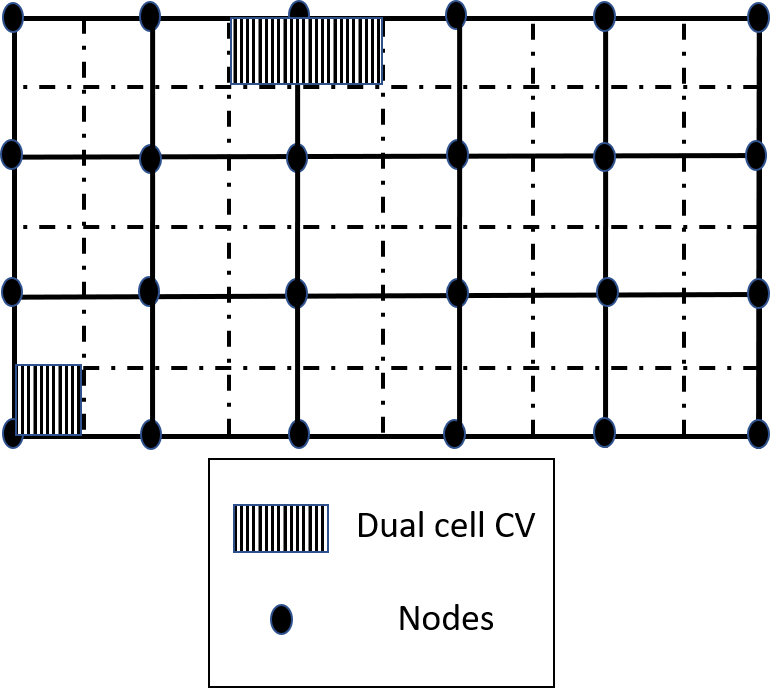
\includegraphics[width=.75\textwidth]{ch3_su2eqn/figures/boundary_dual_cell_nodes.png}
        \caption{Dual cell CV at boundaries.}
        \label{fig:bddualcell}
    \end{subfigure}
    ~ %add desired spacing between images, e. g. ~, \quad, \qquad, \hfill etc. 
      %(or a blank line to force the subfigure onto a new line)
    \begin{subfigure}[b]{0.45\textwidth}
    \centering
    \captionsetup{justification=centering}
        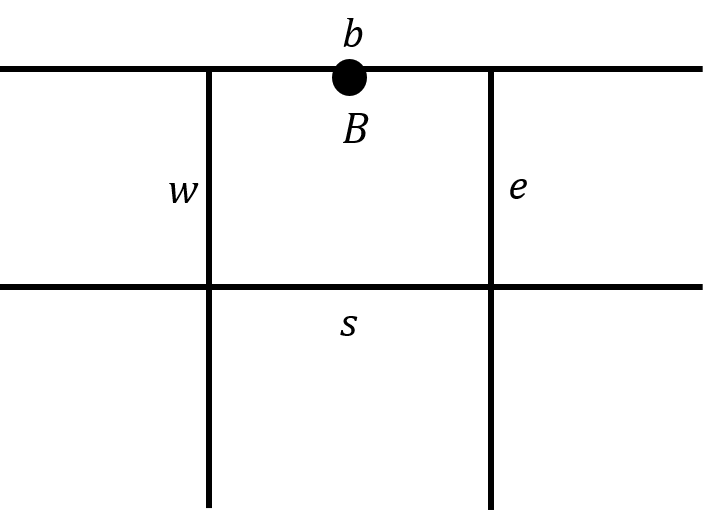
\includegraphics[width=0.75\textwidth]{ch3_su2eqn/figures/boundary_2ddomain.png}
        \caption{Boundary CV discretization.}
        \label{fig:bd2dd}
    \end{subfigure}
    \caption{Control Volume around boundary nodes.}
\end{figure}
While the discretization for the interior faces proceeds as described earlier, the discretization for the boundary face will be presented in this section. Since the boundary node ($B$) is directly on the boundary face ($b$) (figure~\ref{fig:bd2dd}), there is no need to use the momentum interpolation to find the velocity at the face, i.e. for any quantity $\phi$
\begin{equation}
\phi_b = \phi_B.
\end{equation}

The boundary conditions available are free slip wall, no slip wall, velocity inlet, pressure outlet and symmetry boundaries. The application of each of these boundary conditions for the momentum equations, mass flux computation and pressure correction equation is described below.
\subsection{Momentum equations}
\begin{enumerate}
    \item Slip wall: This boundary condition specifies a zero normal flux across the boundary (e.g. inviscid wall). For the momentum equations, this is applied as a weak boundary condition with zero flux across the face. The mass flux across the face is also set to zero.
\begin{equation}
\dot{m}_b = 0.
\end{equation}
    \item Wall (no-slip): This is a strong boundary condition and is generally used to impose a no slip condition on the velocities at the wall. Since the discretization is vertex-based the boundary node lies on boundary face and thus the velocity boundary condition can be enforced as a Dirichlet boundary condition. The mass flux across the face is set to zero and the velocity at the wall is set to zero or to the specified wall velocity ($u_{wall}$).
\begin{equation}
\dot{m}_b = 0, \quad u_b = u_{wall}.
\end{equation}
    \item Inlet: For a prescribed velocity ($u_{in}$) at the inlet, the velocity is imposed as a Dirichlet boundary condition similar to the wall boundary. However, the mass flux is not zero but can be easily computed based on the specified velocity $u_{in}$.
\begin{equation}
\dot{m}_b = \rho u_{i,in} n_i \Delta S_{b}, \quad u_b = u_{in}.
\end{equation}
    \item Outlet: For a specified pressure outlet, a weak boundary condition is applied for the velocities at the outlet. Fully developed flow conditions are assumed at the outlet. Thus, the velocity gradient normal to the outlet surface is zero. Similarly, the mass flux across the face is also computed using the latest estimate of the velocity.
    \begin{equation}
\dot{m}_b = \rho u_{i,b}n_i\Delta S_{b}.
\end{equation}
    \item Symmetry: A symmetry boundary does not only imply a zero flux across the face but also a reflection of the solution state across the boundary face. Consequently, a reflected state of the current state is computed and a Neumann boundary condition is applied. The mass flux across the face is set to zero.
    \item Far-field: Far-field boundaries are typically used in external flow simulations to denote the free-stream conditions. This is treated as an inlet-outlet type boundary where a Dirichlet condition is used for incoming flow and a Neumann boundary for outgoing flow based on the nature of the flux at the boundary face. The mass flux at the far-field face is computed as 
\begin{equation}
\dot{m}_b = \rho u_{i,b}n_i\Delta S_{b}.
\end{equation}
Depending on the sign of the mass flux, this face is treated as an inlet ($\dot{m}_b < 0$) or an outlet ($\dot{m}_b>0$). Implementation of these two conditions are similar to the inlet and outlet boundary conditions.
    \item Periodic: The periodic pair of elements are treated as an internal element by exchanging the flux across the interface. The solution is only computed for the donor node and is transformed back to the receiver node.
\end{enumerate}{}

\subsection{Pressure correction equations}
If the pressure at a particular boundary is unknown (Euler wall, Wall, Inlet, Symmetry) it is treated as a Neumann boundary and the value of the pressure is updated based on the pressure correction. However, if the value of the pressure is specified (Outlet with a specified pressure), the value of the pressure is fixed and the pressure correction is set to zero as a Dirichlet boundary condition.

%\subsection{Turbulence modeling}

%\textcolor{red}{[***May be it better to just mention the turbulence models within a paragraph***]}

%SU2 currently supports two RANS models - the Spalart-Allmaras(S-A) and the Mean Shear Stress Transport (SST) model are linked to the solver. 

%\nomenclature[A]{$C_d$}{Drag coefficient}
%\nomenclature[A]{$P$}{Pressure}
%\nomenclature[A]{$\vec{n}$}{Normal vector}
%\nomenclature[A]{$C_f$}{Skin friction coefficient}
%Here it is assumed $U_{f}^{n}=1/2(U_{P}^{n}+U_{E}^{n})$. This assumption is not valid at every time step and requires further attention. For now, the solution from the momentum equation is only an estimate which will be corrected based on the equation to be derived soon and at convergance when velocity field obeys both continuity and momentum equations, the assumption becomes valid and neglecting the term may be justified. However, this is a workaround and further attention is required

\section{Unsteady problems: Dual time stepping}
Unsteady problems are solved with a dual time stepping scheme. The unsteady problem is converted to a steady state problem within each time step which is solved as described previously. A pseudo transient term is added to equation~\ref{eq:fvmeqn} as
\begin{equation}
\int_{\Omega}\frac{\partial U}{\partial \tau}d\Omega + \int_{\Omega}\frac{\partial U}{\partial t}d\Omega + R(U) = -F^p \rightarrow \int_{\Omega}\frac{\partial U}{\partial \tau}d\Omega + R^{\ast}(U) = 0,
\label{eq:dualtime1}
\end{equation}
where $\tau$ is the pseudo time variable. The pseudo time term is discretized as explained in section~\ref{sssec:timediscr} and the unsteady time term is discretized by a backward Euler scheme. First and second order time integration schemes can be used for the unsteady term. For the first order discretization, $R^{\ast}(U)$ is
\begin{equation}
R^{\ast}(U) = \frac{U-U^n}{\Delta t}|\Omega| + R(U) + F^{p,n},
\end{equation}
and for second order,
\begin{equation}
R^{\ast}(U) = \frac{3U -4U^n +U^{n-1}}{2\Delta t}|\Omega| + R(U) + F^{p,n}.
\end{equation}
At the end of the pseudo-steady solution $U$ of equation~\ref{eq:dualtime1} becomes $U^{n+1}$.
\section{Moving grids}\label{sec:roteqn}
Recall the general form of equations in SU2 from equation~\ref{eq:generic} is 
\begin{equation*}
\frac{\partial U}{\partial t}  + \frac{\partial F^c_i}{\partial x_i}-\frac{\partial F^v_i}{\partial x_i}=Q \quad \text{in} \quad \Omega, \quad t>0.
\end{equation*}
\subsection{Arbitrary Lagrangian Eulerian method}
For the Arbitrary Lagrangian and Eulerian (ALE) formulation, the convective term is expressed as
\begin{equation}
F^c_i = \rho (u_i -u_{g,i})u_j,
\end{equation}
where $u_{g,i}$ is the grid velocity. The other terms remain the same. However, the computation of mass flux at the faces of control volumes must also account for the grid movement. Thus, the relative velocity at a face, $u_{rel,f}$, computed using the Rhie-Chow interpolation is 
\begin{equation}
u_{rel,f}^{\ast}=\overline{u_{f}}^{\ast} - \overline{u}_{f,g} -\overline{\boldsymbol{D}}^{n,u}_f\left(\left(\frac{\partial p^{\prime}}{\partial x}\right)_{f}-\overline{\left(\frac{\partial p^{\prime}}{\partial x}\right)_{f}}\right) + \left(u_{e}^n - \overline{u}_{e}^n\right).
\label{eq:velatfmov}
\end{equation}
Here $\overline{u}_{f,g}$ is the linearly interpolated grid velocity at the face $f$.
\subsubsection{Rotating reference frame}
For steady simulations, in a rotating reference frame with rotation rate $\Omega_i$, the grid velocity can be found as the cross product of the rotation rate vector and the radius vector.
\begin{equation}
u_{g,i} = \epsilon_{ijk} \Omega_i r_j\hat{e}_k.
\end{equation} 
The $\Omega_i$ is the vector of rotation rate about each of the axis, $r_j$ is the radius vector from the center of rotation, $\hat{e}_k$ is the unit coordinate vector and $\epsilon_{ijk}$ is the levi civita tensor. In addition to accounting for grid movement like described above an additional source term is added to the momentum equations
\begin{equation}
Q_{rot} = -\rho \epsilon_{ijk} \Omega_i u_j\hat{e}_k.
\end{equation}
This source term is the cross product of the rotation rate vector, $\Omega_i$, and the velocity vector, $u_j$.
\section{Turbulence modeling}
Turbulence modeling in SU2 is based on solving the Reynolds Averaged Navier Stokes (RANS) equations. As described in section~\ref{ssec:incomprans}, the most widely used approach is to use the Boussinesq hypothesis and write the Reynolds stresses in terms of mean flow gradients. This introduces a new unknown, the turbulent eddy viscosity, $\mu_t$. In order to close the system of RANS equations, equations for the turbulent eddy viscosity are solved. Eddy viscosity turbulence models implemented in SU2 are the Spalart-Allmaras (SA)~\cite{spalart1992one} and the Menter Shear Stress Transport (SST)~\cite{menter1994two} model. These are described in detail in this section.

\subsection{Spalart-Allmaras (SA)}
%\noindent
The SA eddy viscosity model is a one equation model and solves for a scalar variable $\tilde{\nu}$. This scalar is related to the eddy viscosity as
\begin{equation}
\mu_{tur} = \rho \tilde{\nu} f_{v1}.
\end{equation}
Here $\rho$ is the density and $f_{v1}$ is obtained from the turbulence model. Many different versions of the SA turbulence models are available~\cite{NASATMR}. The general form of the equation in all versions closely resembles the transport equation like equation~\ref{eq:genphi}. The standard SA model is
\begin{align}
\frac{\partial \tilde{\nu}}{\partial t} + u_j\frac{\partial \tilde{\nu}}{\partial x_j} = c_{b1}(1-f_{t2})\tilde{S}\tilde{\nu}-\left[c_{w1}f_w - \frac{c_{b1}}{\kappa^2}f_{t2} \right]\left(\frac{\tilde{\nu}}{d}\right)^2 \\+ \frac{1}{\sigma}\left[\frac{\partial}{\partial x_j}\left(\nu_{tot}\frac{\partial \tilde{\nu}}{\partial x_j}\right) + c_{b2}\frac{\partial \tilde{\nu}}{\partial x_i}\frac{\partial \tilde{\nu}}{\partial x_i}\right].\nonumber
\label{eq:saorig}
\end{align}
The definitions of the functions are
\begin{align}
f_{v1} &= \frac{\chi^3}{\chi^3 + c_{cv1}^2}, \nonumber \\
\chi &= \frac{\tilde{\nu}}{\nu},
\end{align}
where $\nu$ is the molecular kinematic viscosity. Additionally,
\begin{equation}
\tilde{S} = \Omega + \frac{\tilde{\nu}}{\kappa^2 d^2}f_{v2}.
\end{equation}
Here $\Omega$ is the magnitude of the vorticity, $d$ is the distance from the point to the nearest wall and
\begin{align}
f_{v2} = 1 - \frac{\chi}{1+\chi f_{v1}}.\nonumber 
\end{align}
$f_w$ is computed as
\begin{align}
f_w &= g\left[\frac{1+c_{w3}^6}{g^6+c_{w3}^6}\right]^{1/6},  \\
g = r + c_{w2}(r^6-r), &\quad r = \text{min}\left(\frac{\tilde{\nu}}{\tilde{S}\kappa^2d^2},10\right) \nonumber.
\end{align}
Finally, $f_{t2}$ is computed as
\begin{align}
f_{t2} = c_{t3}e^{-c_{t4}\chi^2} \nonumber.
\end{align}
The model constants are
\begin{align}
c_{b1} = 0.1355, \quad \sigma=2/3, \quad c_{b2} = 0.622, \nonumber \\
\kappa = 0.41, \quad c_{w2} = 0.3, \quad c_{v1} = 7.1, \\
c_{t3} = 1.2, \quad c_{t4} = 0.5, c_{w1} = \frac{c_{b1}}{\kappa^2} + \frac{1+c_{b2}}{\sigma}. \nonumber
\end{align}
The most widely used version of SA however ignores the trip term $f_{t2}$. This is referred to as the "no trip term" version of the SA turbulence model and is also used in SU2. In this variation the constant $c_{t3}$ is set to zero. The no trip SA turbulence model can now be written in the general form of equation~\ref{eq:generic} as 
\begin{equation*}
\frac{\partial U}{\partial t}  + \frac{\partial F^c_i}{\partial x_i}-\frac{\partial F^v_i}{\partial x_i}=Q \quad \text{in} \quad \Omega, \quad t>0,
\end{equation*}
where
\begin{align}
    U= \Tilde{\nu}, \qquad
    F^c_i = u_i \Tilde{\nu}, \qquad
    F^v_i = \frac{(\nu + \Tilde{\nu})}{\sigma}\frac{\partial \Tilde{\nu}}{\partial x_i} \nonumber, \\
    Q =  c_{b1}\Tilde{S}\Tilde{\nu} -c_{w1}f_w\big(\frac{\Tilde{\nu}}{d_S} \big)^2 + \frac{c_{b2}}{\sigma}\bigg|\frac{\partial \Tilde{\nu}}{\partial x_i}\bigg|^2.
    \label{eq:SAmodel}
\end{align}{}

\subsubsection{Discretization}
Since the turbulence model equation resembles the general scalar transport equation~\ref{eq:genphi}, the discretization is carried out as described in section~\ref{sec:ch2disceqnphi}. Since equation~\ref{eq:SAmodel} is solved sequentially after the momentum and pressure correction equations, the previously solved velocity field is used and the advective term, $F^c_i$ is discretized using an upwind scheme. The viscous term, $F^v_i$, is discretized using a central difference scheme. The source term is discretized using the midpoint integration rule where the gradients are computed with Green-Gauss theorem or the Least Squares method. 

\subsubsection{Boundary conditions}
The most important boundary conditions for the turbulence models are at the walls and far-field boundaries. The boundary condition for the SA turbulence model at the far-field boundaries is
\begin{equation}
\tilde{\nu}_{\infty} = 3 \nu_{\infty}\quad \text{to}\quad 5\nu_{\infty}, 
\end{equation}
and on solid walls 
\begin{equation}
\tilde{\nu} = 0.
\end{equation}
\subsection{Menter Shear Stress Transport (SST)}
The Menter Shear Stress Transport equation~\cite{menter1994two} is a two equation model for finding the turbulent eddy viscosity. The two equations solve for the turbulent kinetic energy, $k$ and specific dissipation rate, $\omega$. This formulation combines two popular two equation models - the $k$-$\omega$ turbulence model~\cite{wilcox1988komega,wilcox2008komega} and the $k$-$\epsilon$ turbulence model~\cite{launder1974kepsilon,jones1972kepsilon} with an additional correction for adverse pressure gradients. The $k$-$\omega$ formulation is used in the inner parts of the boundary layer and $k$-$\epsilon$ formulation in the remaining parts of the flow field. 
The two equations are
\begin{equation}
\frac{\partial \rho k}{\partial t} + \frac{\partial \rho u_j k}{\partial x_j} = P - \beta^* \rho\omega k + \frac{\partial}{\partial x_j}\left((\mu + \sigma_k \mu_t)\frac{\partial k}{\partial x_j} \right),
\label{eq:keqn}
\end{equation}
and
\begin{align}
\frac{\partial \rho\omega}{\partial t} + u_j\frac{\partial \rho u_j \omega}{\partial x_j} = \frac{\partial}{\partial x_j}\left((\mu + \sigma_k \mu_t)\frac{\partial \omega}{\partial x_j} \right) + \frac{\gamma}{\nu_t}P \\ -\beta \rho \omega^2 + 2(1-F_1)\frac{\rho\sigma}{\omega}{\frac{\partial k}{\partial x_i}}{\frac{\partial \omega}{\partial x_i}}.
\label{eq:omeqn}
\end{align}
Here $P$ is the production term given by
\begin{equation}
P = \tau_{ij} \frac{\partial u_i}{\partial x_j}.
\end{equation}
where $\tau_{ij}$ is the viscous stress tensor (equation~\ref{eq:viscstress}). The turbulent eddy viscosity is computed as
\begin{equation}
    \mu_t = \frac{\rho a_1 k}{\text{max}(a_1 \omega, \Omega F_2)},
    \label{eq:kweddyvisc}
\end{equation}{}
where $\rho$ is density, $\Omega$ is the vorticity magnitude, $\Omega = \sqrt{2W_{ij}W_{ij}}$ with 
\begin{equation*}
    W_{ij} = \frac{1}{2}\left(\frac{\partial u_i}{\partial x_j} - \frac{\partial u_j}{\partial x_i} \right).
\end{equation*}{} 
Every constant in the model is a blend of inner and outer value, blended as
\begin{equation*}
    \phi = \phi_1 F_1 + (1 - F_1)\phi_2,
\end{equation*}
where $\phi$ represents any of the constants defined in equation~\ref{eq:kwconst}. The blending functions are computed as
\begin{align*}
    &F_1 = tanh(arg_1 ^4), \\
    &arg_1 = min\Bigg[max\bigg(\frac{\sqrt{k}}{\beta^* \omega d}, \frac{500\nu}{d^2 \omega}\bigg), 
                     \frac{4\rho\sigma_{\omega_2} k}{CD_{k\omega}d^2}\Bigg], \\
    &CD_{k\omega} = max\bigg(2\sigma_{\omega_2}\frac{1}{\omega}\frac{\partial k}{\partial x_j}\frac{\partial \omega}{\partial x_j} ,10^{-20} \bigg), \\
    &F_2 = tanh(arg_2 ^4), \\
    &arg_2 = max\Bigg(2\frac{\sqrt{k}}{\beta^* \omega d}, \frac{500\nu}{d^2 \omega}\Bigg),
\end{align*}
with $d$ being the distance of any field point to the nearest wall.

The constants of the model are given by
\begin{align}{}
a_1 = 0.31, \quad \kappa = 0.41, \quad  \beta^* = 0.09,  \nonumber\\
\sigma_{k_1} = 0.85, \quad \sigma_{\omega_1} = 0.5, \quad \beta_1 = 0.075, \nonumber\\
\sigma_{k_2} = 1.0, \quad \sigma_{\omega_2} = 0.856, \quad  \beta_2 = 0.0828, \nonumber\\
\gamma_1 = \frac{\beta_1}{\beta^*} - \frac{\sigma_{\omega_1}\kappa^2}{\sqrt{\beta^*}}, \quad \gamma_2 = \frac{\beta_2}{\beta^*} - \frac{\sigma_{\omega_2}\kappa^2}{\sqrt{\beta^*}} \label{eq:kwconst}.
\end{align}
Following the general form of the equations in equation~\ref{eq:generic}, the equations~\ref{eq:keqn} and \ref{eq:omeqn} can be written as
\begin{align}
    U=\begin{bmatrix}{}
    \rho k \\
    \rho\omega
    \end{bmatrix},
    F_i^c = \begin{bmatrix}{}
    \rho u_i k \\
    \rho u_i \omega
    \end{bmatrix},
    F^v_i = \begin{bmatrix}{}
    (\mu + \sigma_k \mu_t) \frac{\partial k}{\partial x_i} \\
    (\mu + \sigma_{\omega} \mu_t) \frac{\partial \omega}{\partial x_i}
    \end{bmatrix} \nonumber \\ \nonumber\\
    Q = \begin{bmatrix}{}
    P - \beta^* \rho\omega k \\
    \frac{\gamma}{\nu_t}P - \beta \rho \omega^2 + 2(1-F_1)\frac{\rho\sigma}{\omega}{\frac{\partial k}{\partial x_i}}{\frac{\partial \omega}{\partial x_i}}
    \end{bmatrix}.
\end{align}{}

\subsubsection{Discretization}
Similar to the SA turbulence model, the advective term, $F^c_i$ is discretized using an upwind scheme, the viscous term, $F^v_i$, using a central scheme and the source term is discretized using the midpoint integration rule with the gradients computed using either the Green Gauss theorem or the Least Squares method. 

\subsubsection{Boundary conditions}
The boundary conditions at the far-field boundaries for the SST $k-\omega$ model are
\begin{align}
k_{\infty}  &= \frac{3}{2} V_{\infty}^2 TI^{2},\nonumber\\
\omega_{\infty} &= \frac{k_{\infty}}{\nu_{\infty}\frac{\mu_t}{\mu_{lam}}}.
\end{align}
Here $\nu_{\infty}$ is the kinematic viscosity in the free stream, $V_{\infty}$ is the free stream velocity magnitude, $\rho$ is the density and $TI$ is the turbulent intensity. The ratio $\mu_t/\mu_{lam}$ and turbulent intensity $TI$ are specified as inputs. 
On solid walls, the boundary conditions are 
\begin{align}
k &= 0, \nonumber \\
\omega &= 10 \frac{6 \nu}{\beta_1(\Delta d)^2}.
\end{align}
$\Delta d$ is the first cell height and $\beta_1$ is a model constant defined earlier.


%%%%%%%%%%%%%%%%%%%%%%%%%%%%%%%%%%%%%%%%%%%

\bibliographystyle{dissertation}
\bibliography{ch3_su2eqn/su2ch3}


%\references{su2references}

\chapter[Verification and Validation]{Verification and Validation}
\label{ch:ch4results}

%% The following annotation is customary for chapter which have already been
%% published as a paper.
\blfootnote{}

\begin{abstract}
%abstract
In this chapter, the different features of the new pressure based solver will be verified and validated against analytical solutions, experimental data and other references. For verification of the solver, problems with an analytical solution like the Taylor-Couette flow and the plane Poisuelle flow will be used. The validation cases presented will be used to test the different features that are typically encountered during external aerodynamics applications. First, laminar flow problems are used to validate the implementation of the flow solver. Then, turbulent flow problems are presented to validate the coupling of the new flow solver with the existing turbulence solvers. Finally, the unsteady behavior of the new solver is validated. Wherever possible the grids for the numerical simulations are taken from standard sources like the NASA turbulence modeling database~\cite{NASATMR} or the SU2 test case repository to avoid any potential sources of error from mesh generation.

Laminar and turbulent boundary layers are extremely crucial in wind turbine aerodynamics and the numerical solutions from the new solver are validated against theoretical boundary layer solutions under both circumstances. Flow separation, though undesirable, occurs frequently and the behavior of the new solver under separated conditions is tested for the flow over a backward facing step for both laminar and turbulent flow conditions. Other representative test cases, like the flow over a cylinder and flow past an airfoil are also presented. Finally, two unsteady cases are considered; a laminar flow past a square cylinder and a turbulent flow past a pitching airfoil undergoing dynamic stall. 
\end{abstract}
\section{Verification} 
In order to verify the accuracy of the solver, Couette flow or the flow between two solid surfaces is simulated. Two special cases are considered here - the flow between two concentric infinitely long rotating cylinders (also known as Taylor-Couette flow, see the figure~\ref{fig:couetteschem}) and a planar flow between two solid infinitely long parallel plates that are held fixed (also known as plane Poisuelle flow, see figure~\ref{fig:channelschem}). An analytical solution for the velocity profile can be found for both these cases which is used to calculate the order of convergence of the solver. 

While an analytical solution is not available for the laminar flow in a lid driven cavity, reference solutions for velocity can be found in literature~\cite{Ghia1982}. Thus, the solutions for the lid driven cavity is also used to compute the order of accuracy.

\subsubsection{Taylor Couette flow}
The schematic of the Taylor-Couette flow is shown in figure~\ref{fig:couetteschem}. 
\begin{figure}[h]
    \centering
    \captionsetup{justification=centering}
    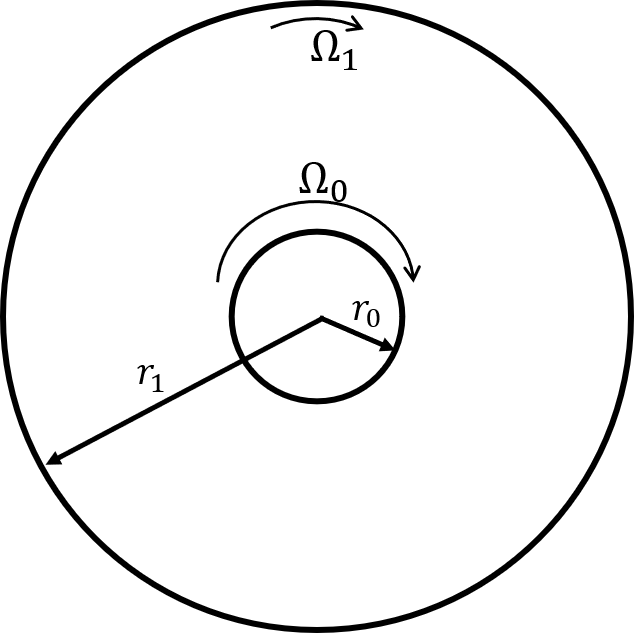
\includegraphics[width=0.25\textwidth]{figures/couette_schem.png}
    \caption{Schematic of the Taylor-Couette flow.}
     \label{fig:couetteschem}
\end{figure}
The inner cylinder has a radius of $r_0$ and the outer radius is $r_1$. $\Omega_0$ and $\Omega_1$ are the angular velocities of the inner and outer cylinders respectively. The analytical solution~\cite{taylor1923viii} for the azimuthal velocity as a function of the radius $r$ is
\begin{equation}
    u_{ana}(r) = r_0 \Omega_0 \frac{r_1/r - r/r_1}{r_1/r_0-r_0/r_1} + r_1 \Omega_1 \frac{r/r_0 - r_0/r}{r_1/r_0-r_0/r_1}.
\end{equation}{}
\begin{figure}[h]
    \centering
     \captionsetup{justification=centering}
    \begin{subfigure}[b]{0.47\textwidth}
    \captionsetup{justification=centering}
        \includegraphics[width=1.0\textwidth]{figures/Velocity_Couette.eps}
        \caption{Velocity vs radial distance.}
        \label{fig:couettevel}
    \end{subfigure}
    ~ %add desired spacing between images, e. g. ~, \quad, \qquad, \hfill etc. 
      %(or a blank line to force the subfigure onto a new line)
    \begin{subfigure}[b]{0.47\textwidth}
    \centering
    \captionsetup{justification=centering}
        \includegraphics[width=1.0\textwidth]{figures/Error_Couette.eps}
        \caption{Order of convergence.}
        \label{fig:couetteerr}
    \end{subfigure}
    \caption{Grid convergence for the Taylor Couette flow.}
\end{figure}

The simulation was carried out on a domain with $r_0 = 1m$ and $r_1=5m$. The outer wall is held fixed ($\Omega_1 = 0$) and the inner wall is rotating at an angular velocity $\Omega_0 = 1$ rad$/$s. The two solid walls are treated as moving wall boundaries. Three different grid resolutions are considered with $16$, $32$ and $64$ cells along the radial direction and with $40$ nodes along the circumference of the cylinders. Uniform grid spacing is used in all cases. 

Figure~\ref{fig:couettevel} shows the comparison between the numerical and analytical velocity profile. The numerical solution matches the analytical solution for all the grid resolutions very well. The numerical error is computed as 
\begin{equation*}
e_{num} = |u_{ana} - u_{num}|.
\end{equation*} 
Figure~\ref{fig:couetteerr} shows the $log_{10}$ of the $L_2$ norm of the error plotted against the number of points in the radial direction.  The numerical error decreases at a rate of $1.938$ indicating an approximately second order rate of convergence as the grid size is halved.

\paragraph{Convergence behavior}
The residual history for the grids with $32$ and $64$ nodes are plotted in figures~\ref{fig:couetteres32} and \ref{fig:couetteres64}. The residuals of both the velocity components and the mass flux, which serves as the indicator for convergence of the continuity equation, all converge within $1200$ iterations for the coarser grid and about $4400$ iterations for the fine grid.
\begin{figure}[h]
    \centering
     \captionsetup{justification=centering}
    \begin{subfigure}[b]{0.48\textwidth}
    \captionsetup{justification=centering}
        \includegraphics[width=1.0\textwidth]{figures/couette_conv_32.eps}
        \caption{$40\times32$ grid.}
        \label{fig:couetteres32}
    \end{subfigure}
    ~ %add desired spacing between images, e. g. ~, \quad, \qquad, \hfill etc. 
      %(or a blank line to force the subfigure onto a new line)
    \begin{subfigure}[b]{0.48\textwidth}
    \centering
    \captionsetup{justification=centering}
        \includegraphics[width=1.0\textwidth]{figures/couette_conv_64.eps}
        \caption{$40\times64$.}
        \label{fig:couetteres64}
    \end{subfigure}
    \caption{Convergence history for the Taylor Couette flow residual.}
\end{figure}
The two velocity components converge identically because of rotational symmetry.

\subsubsection{Plane Poisuelle flow}
The plane Poisuelle flow is the flow between two infinitely long parallel plates that are held fixed (figure~\ref{fig:channelschem}). The boundary conditions used for the simulation are shown in figure~\ref{fig:channelbcs}. At the inlet boundary, a uniform velocity profile is prescribed, and a zero velocity gradient at the outlet is specified. The outlet pressure is set to zero. A small symmetry region is present immediately after the inlet before the channel starts.
\begin{figure}[h!]
    \centering
    \captionsetup{justification=centering}
    \begin{subfigure}[b]{0.47\textwidth}
    \centering
    \captionsetup{justification=centering}
    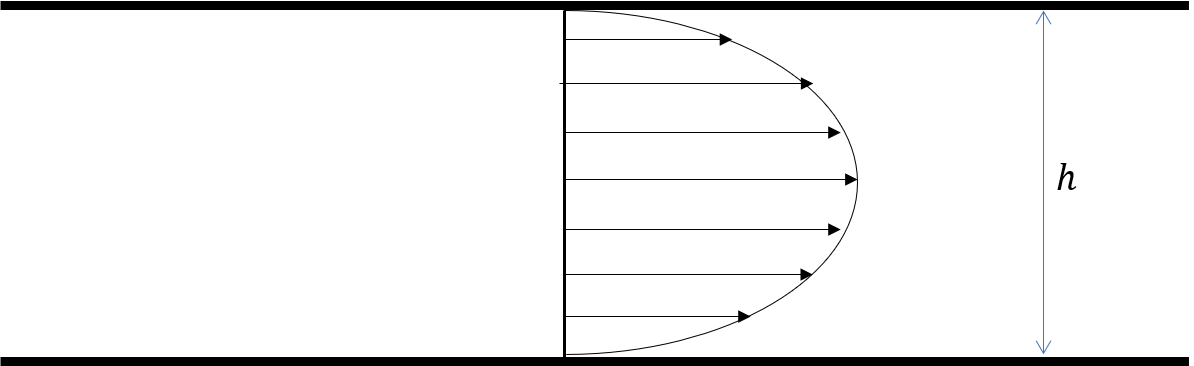
\includegraphics[width=1.0\textwidth]{figures/channel_schem.png}
    \caption{Schematic of the plane Poisuelle flow.}
     \label{fig:channelschem}
    \end{subfigure}
    ~ %add desired spacing between images, e. g. ~, \quad, \qquad, \hfill etc. 
      %(or a blank line to force the subfigure onto a new line)
    \begin{subfigure}[b]{0.47\textwidth}
    \centering
    \captionsetup{justification=centering}
     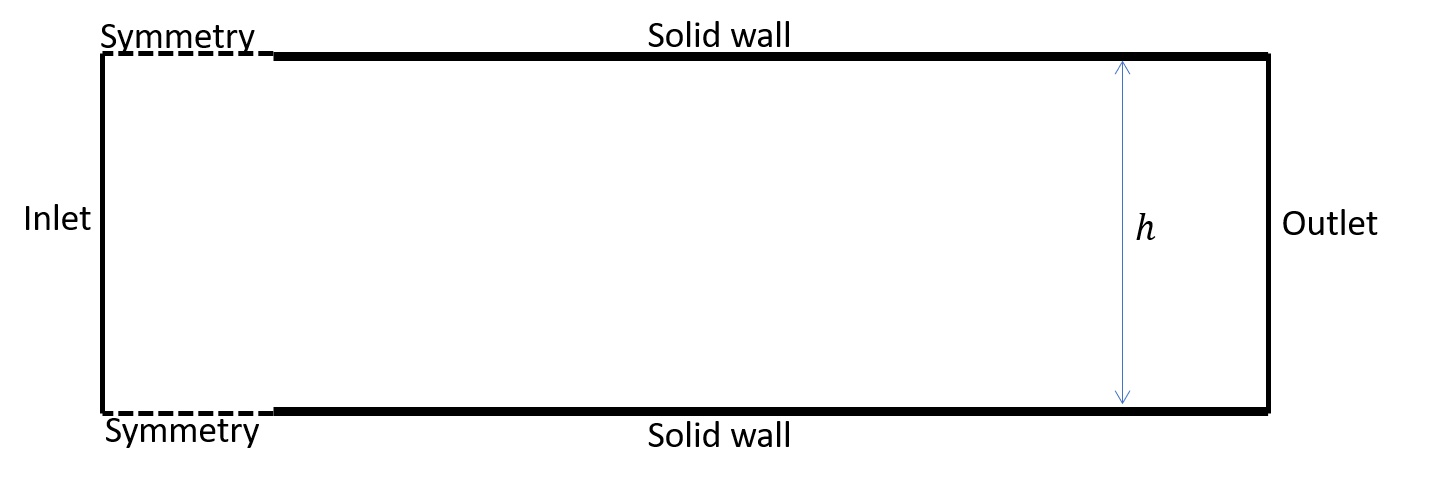
\includegraphics[width=1.0\textwidth]{figures/channel_bcs.png}
    \caption{Domain and boundary conditions.}
     \label{fig:channelbcs}
    \end{subfigure}
    \caption{(a) Schematic of the plane Poisuelle flow and (b) the domain and boundary conditions for the numerical simulation.}
\end{figure}
The plane Poisuelle flow at a mean flow Reynolds number based on channel width $h$ and inlet velocity $U_{in}$ of $Re = \frac{h U_{in}}{\nu} = 400$ is considered. For fully developed flow conditions, the axial velocity profile at any location $y$ can be computed as
\begin{equation}
    u(y)=-\frac{dP}{dx}\frac{1}{2\mu}y(y-h),\qquad 0\leq y \leq h
\end{equation}{}

\noindent where $\frac{dP}{dx}$ is the constant pressure gradient in the streamwise direction, $\mu$ is the laminar viscosity and $h$ is the channel width.
The domain is $1.25 m$ long in the streamwise direction with a symmetry region of $0.25 m$ after the inlet boundary. The distance between the two solid walls is $h=0.125 m$ (figure~\ref{fig:channelbcs}). Four different mesh resolutions are chosen with $16$, $32$, $64$ and $128$ elements in the direction normal to the solid walls and $100$ elements in the streamwise direction. 

\begin{figure}[h!]
    \centering
    \captionsetup{justification=centering}
    \begin{subfigure}[b]{0.45\textwidth}
    \centering
    \captionsetup{justification=centering}
        \includegraphics[width=1.0\textwidth]{figures/channel_vel.eps}
        \caption{Velocity comparison.}
        \label{fig:chvelcmp}
    \end{subfigure}
    ~ %add desired spacing between images, e. g. ~, \quad, \qquad, \hfill etc. 
      %(or a blank line to force the subfigure onto a new line)
    \begin{subfigure}[b]{0.45\textwidth}
    \centering
    \captionsetup{justification=centering}
        \includegraphics[width=1.0\textwidth]{figures/channel_l2.eps}
        \caption{$L_2$ norm of the error}
        \label{fig:chl2}
    \end{subfigure}
    \caption{(a) Comparison of numerical and analytical results. (b) Error as a function of number of cells.}
\end{figure}
Figure~\ref{fig:chvelcmp} shows the comparison of the streamwise velocity at $x=0.9$, which is $7.2h$ away from the start of the channel, as a function of the normal distance for different grid resolutions against the analytical solution. The flow is fully developed after roughly $5h$ to $6h$ from the start of the channel. The pressure gradient required to compute the numerical solution is obtained from the results of the finest grid with $128$ elements in the normal direction. The numerical results from all the grids match the analytical solution closely. The error between the numerical solution and the analytical solution is computed for the three meshes with $16$, $32$ and $64$ elements. The $L_2$ norm of the error is plotted against the number of elements in the normal elements in the figure~\ref{fig:chl2} on a log scale. The slope of the error curve is $2.1$.

\paragraph{Convergence behavior}
\begin{figure}[h]
    \centering
    \captionsetup{justification=centering}
    \begin{subfigure}[b]{0.47\textwidth}
    \captionsetup{justification=centering}
        \includegraphics[width=1.0\textwidth]{figures/channel_conv_hist.eps}
        \caption{SIMPLE convergence history.}
        \label{fig:channelhist}
    \end{subfigure}
    ~ %add desired spacing between images, e. g. ~, \quad, \qquad, \hfill etc. 
      %(or a blank line to force the subfigure onto a new line)
    \begin{subfigure}[b]{0.47\textwidth}
    \centering
    \captionsetup{justification=centering}
        \includegraphics[width=1.0\textwidth]{figures/channel_conv_comparison.eps}
        \caption{SIMPLEC and SIMPLE.}
        \label{fig:channelcmp}
    \end{subfigure}
    \caption{Plane Poisuelle flow  (a) residual convergence history on the $100\times64$ grid and (b) comparsion of convergence behavior for SIMPLE and SIMPLEC for the streamwise velocity on the $100\times64$ grid.}
\end{figure}
Figure~\ref{fig:channelhist} shows the convergence history for the two velocity components and the mass flux for the SIMPLE algorithm. Convergence is achieved in $630$ iterations. Figure~\ref{fig:channelcmp} shows the comparison of residual convergence of the streamwise velocity component for the SIMPLE and SIMPLEC iterative methods. Since the pressure corrections are under-relaxed appropriately, there is no significant difference in convergence behavior. However, SIMPLEC does converge slightly faster in this case.

\subsubsection{Lid driven cavity}
The flow within a lid driven cavity is a commonly used validation problem for CFD solvers. The domain consists of a square cavity with the top wall being moved at a constant velocity along the $x$ axis. This case also serves to test the moving wall boundary condition. While there is no analytical solution for this case, the results from a lid driven cavity are compared against results from Ghia~\cite{Ghia1982}. Ghia~\cite{Ghia1982} solves the vorticity stream function formulation of the incompressible Navier Stokes equations using a multigrid method. The flow is steady and laminar and is a solution of the exact Navier Stokes equation. A square domain $L\times L$ with side $L=1m$ is used. The top wall of the domain is moving at a constant velocity, $U_w$, in the $x$ direction. The flow Reynolds number defined based on the wall velocity, $U_w$ and the length of side of the square lid is $Re= \frac{U_w L}{\nu} = 400$. Three different grids are considered with $33$, $65$ and $129$ nodes along each direction. A uniform grid spacing is used throughout the domain. 
Figure~\ref{fig:ldcgr} shows the $x$ component of the velocity along $x=0.5$ for the three grids and the benchmark results from Ghia~\cite{Ghia1982}. The numerical results improve against the benchmark solution as the grid is refined. Figure~\ref{fig:ldcstr} shows the $L_2$ norm of the error between the results from SU2 and the benchmark solution. The error reduces with a slope of $1.89$ as the grid spacing is halved.
\begin{figure}[h!]
    \centering
    \captionsetup{justification=centering}
    \begin{subfigure}[b]{0.45\textwidth}
    \centering
    \captionsetup{justification=centering}
        \includegraphics[width=1.0\textwidth]{figures/lid_driven_cavity.eps}
        \caption{Velocity at $x=0.5$.}
        \label{fig:ldcgr}
    \end{subfigure}
    ~ %add desired spacing between images, e. g. ~, \quad, \qquad, \hfill etc. 
      %(or a blank line to force the subfigure onto a new line)
    \begin{subfigure}[b]{0.45\textwidth}
     \captionsetup{justification=centering}
        \includegraphics[width=1.0\textwidth]{figures/l2ldc.eps}
%        \includegraphics[width=0.9\textwidth]{figures/lid_driven_cavity_streamlines.png}
        \caption{$L_2$ norm of the error.}
        \label{fig:ldcstr}
    \end{subfigure}
    \caption{(a)Velocity profile comparison between numerical results from SU2 and reference solution~\cite{Ghia1982} at $x=0.5$ and (b) the $L_2$ norm of the error. }
\end{figure}

%Convergence history is also shown for the coarse grid with SIMPLEC and PISO algorithms (Fig. \ref{fig:chconhist}). As expected, the PISO algorithm converges to the final solution faster than the SIMPLEC algorithm.
From both the verification cases with an analytical solution, it is seen that when the number of elements is doubled and subsequently the grid spacing, $\Delta$, is halved, the error is proportional to a factor of approximately $(\Delta)^2$. Also for the lid driven cavity solution where no analytical solution was available, the numerical error when compared against another numerical benchmark result reduced by a factor $(\Delta)^{1.89}$ indicating approximately second order accuracy of the spatial discretization scheme.


\section{Validation}
In this section the numerical results from the new pressure based solver are validated against either experimental data or reference data from other computational methods. The focus will be to test different flow features that are relevant for external aerodynamics.
\subsection{Laminar flows}\label{ssec:blasisus}

\subsubsection{Flow over a flat plate}

Understanding the boundary layer is critical for external aerodynamics. To that end, first the laminar flow over a flat plate with no pressure gradient at a Reynolds number of $Re = 4\times10^5$ is now considered to analyze the behavior of the new solver in capturing the laminar boundary layer. A semi analytical solution, commonly known as the Blasius solution~\cite{schlichting2016boundary}, can be found for the streamwise and normal velocity components under self similar conditions. Self similar solutions can be found by first transforming the coordinates and the velocities as follows
\begin{equation}
x \rightarrow c^2 x, \quad y \rightarrow cy, \quad u \rightarrow u, \quad v \rightarrow \frac{v}{c}.
\end{equation}
Here $c$ is any positive constant. Introducing the new similarity variable $\eta$ and the non dimensional function $f$ as
\begin{equation}
\eta = \frac{y^{\ast}}{\delta(x^{\ast})}, \quad \psi = \sqrt{\nu U x^{\ast}}f(\eta),
\end{equation} 
where $\delta(x)$ is the boundary layer thickness at a location $x$, $U$ is the free stream velocity, $\nu$ is the kinematic viscosity, $\psi$ is the stream function and $f(\eta)$ is a function of the similarity variable only. An ordinary differential equation (ODE) in $f(\eta)$ can then be formed as, see~\cite{schlichting2016boundary} 
\begin{equation}
2f^{\prime\prime\prime} + f^{\prime \prime} f = 0,
\label{eq:blasius}
\end{equation}
where $^{\prime}$ denotes differentiation with respect to the similarity variable $\eta$. The boundary conditions can be derived from the no slip condition at the wall and the matching condition at the edge of the boundary layer.
\begin{align*}
u(x,0) = 0, \quad \rightarrow f^{\prime}(0) = 0, \\
v(x,0) = 0, \quad \rightarrow f(0) = 0, \\
u(x,\infty) = U \quad \rightarrow f^{\prime}(\infty) = 1.
\end{align*}
The velocity components can be written in terms of the stream function $\psi$ and consequently the similarity variable as
\begin{equation}
u(x,y) = \frac{\partial \psi}{\partial y} = U f^{\prime}(\eta), \quad 
v(x,y) = -\frac{\partial \psi}{\partial x} = \frac{1}{2}\sqrt{\frac{\nu U}{x}}[\eta f^{\prime}(\eta) - f(\eta)].
\end{equation}
Additionally, the wall shear stress is given by, 
\begin{equation}
\tau_w = \mu\left(\frac{\partial u}{\partial y}\right)_{y=0} = 0.332\mu U\sqrt{\frac{U}{\nu x}}.
\end{equation}
Using the wall shear stress, the skin friction coefficient, $C_f$, can be found as
\begin{equation}
C_f = \frac{\tau_w}{\frac{1}{2}\rho U^2}, = 0.664\frac{0.664}{\sqrt{Re_x}},
\end{equation}
where $Re_x$ is the local Reynolds number defined as $Re=\frac{U x}{\nu}$. Equation~\ref{eq:blasius} can be solved numerically to find $f(\eta)$ as a function of $\eta$. With that the self similar velocity profiles and the skin friction coefficient can be found which will be used to study the behavior of the new solver in capturing the boundary layer. 

The domain used for the numerical simulations is shown in figure~\ref{fig:lfpdom}. A uniform inflow is prescribed and a small inflow region with a symmetry boundary is used before the flat plate begins. Two different meshes are considered. The coarse mesh has $65$ nodes in both while the fine mesh has $129$ nodes along the streamwise and normal directions. The boundary conditions and the coarse mesh used for the simulation are shown in figures~\ref{fig:lfpdom} and \ref{fig:lfpmesh}. Nodes are clustered near the wall and stretched away from it in the normal direction and clustered around the interface between the symmetry and the wall region and stretched towards the outlet in the streamwise direction (figure~\ref{fig:lfpmesh}). The minimum normal grid spacing in the coarse mesh is $1.60\times10^{-5}m$ and $8.0\times10^{-6}m$ for the fine mesh. Grid spacing at $x=0$ when the wall begins is $0.001m$ in the coarse mesh and $0.0005m$ for the fine mesh
\begin{figure}[h!]
    \centering
    \captionsetup{justification=centering}
    \begin{subfigure}[b]{0.45\textwidth}
    \centering
    \captionsetup{justification=centering}
        \includegraphics[width=\textwidth]{figures/fp_msh.jpeg}
        \caption{Domain and boundary conditions.}
        \label{fig:lfpdom}
    \end{subfigure}
    ~ %add desired spacing between images, e. g. ~, \quad, \qquad, \hfill etc. 
      %(or a blank line to force the subfigure onto a new line)
    \begin{subfigure}[b]{0.45\textwidth}
    \centering
    \captionsetup{justification=centering}
        \includegraphics[trim = 50 50 0 450,clip,width=1.0\textwidth, height=0.35\textwidth]{figures/lamfpdomain.eps}
        \caption{Mesh.}
        \label{fig:lfpmesh}
    \end{subfigure}
    \caption{Flat plate (a) domain and boundary conditions and (b) the $65\times65$ mesh.}
\end{figure}

Figures~\ref{fig:fpux15} and \ref{fig:fpvx15} show the comparison of the streamwise and normal velocity components at $x=0.15m$ against Blasius solution for the two meshes considered. The streamwise component matches very closely with the Blasius solution in both meshes whereas there is a small difference in the normal component of velocity near the edge of the boundary layer. The profile from the fine mesh is closer to the analytical profile. It should also be noted that the normal component of the velocity is significantly smaller than the streamwise component.
\begin{figure}[h!]
    \centering
    \captionsetup{justification=centering}
    \begin{subfigure}[b]{0.47\textwidth}
    \captionsetup{justification=centering}
        \includegraphics[width=\textwidth]{figures/lamfp_ux015.eps}
        \caption{Streamwise component.}
        \label{fig:fpux15}
    \end{subfigure}
    ~ %add desired spacing between images, e. g. ~, \quad, \qquad, \hfill etc. 
      %(or a blank line to force the subfigure onto a new line)
    \begin{subfigure}[b]{0.47\textwidth}
    \centering
    \captionsetup{justification=centering}
        \includegraphics[width=\textwidth]{figures/lamfp_vx015.eps}
        \caption{Normal component.}
        \label{fig:fpvx15}
    \end{subfigure}
    \caption{Comparison of streamwise and normal velocity components to the Blasius solution at $x=0.15$.}
\end{figure}
Figure~\ref{fig:lfpcf} shows the skin friction coefficient from the two meshes compared against the Blasisus solution. A good agreement between the numerical results and theory is found in both cases.
\begin{figure}[h!]
    \centering
    \captionsetup{justification=centering}
    \includegraphics[width=0.5\textwidth]{figures/lamfp_cf.eps}
    \caption{Skin friction coefficient for the laminar flow over the flat plate.}
     \label{fig:lfpcf}
\end{figure}

\subsubsection{Flow over a cylinder}
As a simple test case of external aerodynamics, the flow past a circular cylinder is considered. At low Reynolds numbers, the flow remains steady and laminar~\cite{cylinderref}. The flow separates symmetrically at two points on the cylinder and a recirculation region is formed behind the cylinder. In this study, the drag coefficient and the different flow features (figure~\ref{fig:cylflfeatures}) are compared against a reference numerical solution~\cite{cylinderref}. 
\begin{figure}[h!]
    \centering
    \captionsetup{justification=centering}
    \includegraphics[width=0.6\textwidth]{figures/reattachprop.png}
    \caption{Flow features around a cylinder at a Reynolds number $Re=40$~\cite{cylinderref}.}
     \label{fig:cylflfeatures}
\end{figure}
$L_w$ corresponds to the length of the wake, $(a,b)$ is the location of the recirculation center and $\theta$ is the separation angle on the upper half of the cylinder.

The Reynolds number based on the cylinder diameter is $Re = 40$ and a series of five grids are used to study the properties. The diameter of the cylinder is $D=1m$. The coarsest grid has $65$ nodes on the cylinder. The number of nodes are doubled till $1025$ nodes on the cylinder. The domain extends for $50 D$ to all sides of the cylinder. A freestream boundary condition is imposed on the outer part of the domain. Figure~\ref{fig:cyl40cd} shows the drag coefficient ($C_d$) from the different grids. The values are also listed in table~\ref{tab:lamcylcd}. The solution converges to a value of $1.499$ which is close to the reported value in Gautier et al~\cite{cylinderref}. Figure~\ref{fig:cyl40rec} shows the different flow features. Separation on the upper half occurs around the point $(x,y) = (0.294,0.404)$ (assuming the center of the cylinder lies at $(x,y) = (0,0)$) which corresponds to a separation angle of approximately $\theta = 126^{\circ}$ measured from the leading edge. The center of the recirculation region is at $(1.2,0.295)$ on the upper half and at $(x,y) = (1.2,-0.295)$ on the lower half. The flow features from SU2 and Gautier et al~\cite{cylinderref} are also listed in table~\ref{tab:lamcylfeat}. Like the drag coefficient, the flow features match closely with the reference solution. These flow features are computed on a grid with $513$ nodes on the cylinder as a grid independent solution is obtained at that point.
\begin{figure}[h!]
    \centering
    \captionsetup{justification=centering}
    \begin{subfigure}[b]{0.45\textwidth}
    \captionsetup{justification=centering}
        \includegraphics[width=\textwidth]{figures/cylinder_drag.eps}
        \caption{Grid refinement study of the drag coefficient.}
        \label{fig:cyl40cd}
    \end{subfigure}
    ~ %add desired spacing between images, e. g. ~, \quad, \qquad, \hfill etc. 
      %(or a blank line to force the subfigure onto a new line)
    \begin{subfigure}[b]{0.45\textwidth}
    \centering
    \captionsetup{justification=centering}
        \includegraphics[width=\textwidth]{figures/cylinderreattach.eps}
        \caption{Recirculation region behind the cylinder.}
        \label{fig:cyl40rec}
    \end{subfigure}
    \caption{Laminar flow over a cylinder at $Re =40$.}
\end{figure}
\begin{table}[h!]
\centering
\captionsetup{justification=centering}
\begin{tabular}{ |c|c| } 
\hline
Nodes ($N$) & Drag ($C_d$) \\
\hline
  $65$  & $1.537$ \\ 
 \hline
  $129$  & $1.511$ \\ 
 \hline
 $257$ & $1.502$ \\ 
 \hline
 $513$ & $1.499$ \\ 
 \hline
 $1025$ & $1.499$ \\ 
 \hline
 Gautier et al~\cite{cylinderref} & $1.49$ \\
 \hline
\end{tabular}
\caption{Drag coefficient ($C_d$) for different grid resolutions. $N$ denotes the number of points on the surface of the cylinder.}
\label{tab:lamcylcd}
\end{table}
\begin{table}[h!]
\centering
\captionsetup{justification=centering}
\begin{tabular}{ |c|c|c| } 
\hline
& SU2 & Gautier et al~\cite{cylinderref} \\
\hline
  $L_w/D$  & $2.18$ & $2.24$\\ 
 \hline
  $a/D$  & $0.70$ & $0.71$ \\ 
 \hline
 $b/D$ & $0.59$ & $0.59$\\ 
 \hline
 $\theta$ & $126^{\circ}$ & $126.4^{\circ}$\\ 
 \hline
\end{tabular}
\caption{Flow features for flow around a cylinder at a Reynolds number of $Re=40$.}
\label{tab:lamcylfeat}
\end{table}

Richardson's extrapolation formula~\cite{richardsonext}
\begin{equation}
C_d(h/t) - C_d(h/s) \approx \frac{C_d(h/s) - C_d(h)}{s^k-1} - \frac{C_d(h/t) - C_d(h)}{t^k-1}
\end{equation}
can be used on the drag values in table~\ref{tab:lamcylcd} to find the approximate order of convergence. Here $h$ is the starting grid size, $t$ and $s$ are two integer factors and $k$ is the order of convergence. The grid size $h$ can be found for each case as $\pi D/(N-1)$ where $D$ is the cylinder diameter, $\pi D$ is the circumference of the cylinder and $N$ is the number of nodes on the cylinder. The results are shown in table~\ref{tab:lamcylord}. The drag coefficient converges at a rate of approximately $1.5$.
\begin{table}[h!]
\centering
\begin{tabular}{ |c|c|c|c| } 
\hline
 $N$ & $t$ & $s$ & $k$\\
\hline
  $65$  & $2$ & $4$ &$1.53$\\ 
 \hline
  $129$  & $2$ & $4$ & $1.58$\\ 
 \hline
 $65$ & $4$ & $8$&$1.56$\\ 
 \hline
\end{tabular}
\caption{Order of convergence of the drag coefficient using Richardson's extrapolation for the flow over a cylinder at $Re = 40$.}
\label{tab:lamcylord}
\end{table}

\subsubsection{Flow over a backward facing step}
Flow separation occurs commonly in external aerodynamics. In the previous case of the flow over the cylinder, the separation location was validated against reference data. In this section, the behavior of the flow within the separated region is tested by analyzing the flow over a backward facing step. The domain consists of an inlet channel which expands into a larger channel across a step. The flow separates at the step and re-attaches downstream along the lower wall. Unlike the flow past a cylinder, here the flow separation occurs at a fixed point, namely at the corner of the step removing any uncertainty in the location of the separation point. Depending on the Reynolds number, a secondary separated region can also occur along the top wall. A Reynolds number of $Re=800$ based on the step height is considered and the flow is expected to separate along both the bottom and top walls. The numerical results are compared to results from Gartling~\cite{gartling4}. 

The outline of the domain used is shown in figure~\ref{fig:lambfsstr}. The step height is $0.5m$ and the channel height is $1m$. The step and the inlet is located on the left boundary at $x=0$ as shown in the figure~\ref{fig:lambfsstr}. The step starts at $y=-0.5$ and extends upto $y=0$. The region from $y=0$ to $y=0.5$ is treated as an inlet boundary and a fully developed velocity profile is imposed there. Three different meshes are considered with uniform grid resolutions of $121\times17$, $241\times33$ and $481\times65$ nodes in the streamwise and normal direction, respectively. At the outlet, the pressure is prescribed to be zero.
\begin{figure}[h!]
    \centering
    \captionsetup{justification=centering}
    \includegraphics[trim=0 0 0 350,clip,width=0.9\textwidth]{figures/streamlines_lambfs_cut.png}
    \caption{Streamlines for the laminar backward facing step at $Re=800$.}
     \label{fig:lambfsstr}
\end{figure}
 

\begin{figure}[h!]
    \centering
    \captionsetup{justification=centering}
    \begin{subfigure}[b]{0.48\textwidth}
    \captionsetup{justification=centering}
        \includegraphics[width=\textwidth]{figures/lam_bfs_x7.eps}
        \caption{Streamwise velocity at $x=7m$.}
        \label{fig:bfsx7}
    \end{subfigure}
    ~ %add desired spacing between images, e. g. ~, \quad, \qquad, \hfill etc. 
      %(or a blank line to force the subfigure onto a new line)
    \begin{subfigure}[b]{0.48\textwidth}
    \centering
    \captionsetup{justification=centering}
        \includegraphics[width=\textwidth]{figures/lam_bfs_x15.eps}
        \caption{Streamwise velocity at $x=15m$.}
        \label{fig:bfsx15}
    \end{subfigure}
    \caption{Comparison of the streamwise velocity profiles obtained from the numerical results with the literature at (a) $x=7m$ and (b) $x=15m$.}
    \label{fig:bfsvel}
\end{figure}
Figure~\ref{fig:bfsvel} compares the numerical and experimental results for the streamwise velocity component at two different locations for the three meshes.  Figure~\ref{fig:bfsx7} shows the velocity at $x=7m$. This is within the recirculation region and the flow is separated at the upper wall. The coarse mesh ($121\times17$) performs poorly at this location. The results from the finest mesh ($481\times65$) agree very well with the experimental data. Figure~\ref{fig:bfsx15} shows the same comparison at $x=15m$. This location is after the flow has reattached on both the upper and lower walls. As a consequence, the performance of the coarse mesh improves and the other two meshes also give very good results. The length of the recirculating zone along the lower wall is $5.81m$ and along the upper wall is $5.69m$ which match the results from Gartling~\cite{gartling4}.


\subsection{Turbulent flows}\label{ssec:turbprofile}
Most flows of practical interest are turbulent and in this section the behavior of the new solver in turbulent conditions will be validated.
\subsubsection{Flow over a flat plate}
%\paragraph{Turbulent boundary layer velocity profiles}
The turbulent boundary layer can be broadly divided into two regions \cite{Pope2000,schlichting2016boundary}: the inner region where viscous dissipation is present and the outer region where the turbulence dissipation dominates completely. The inner region consists of the viscous sub-layer where viscous effects dominate and turbulent effects are absent, a buffer region where the turbulent stresses start to grow and finally an overlap or logarithmic region where the turbulent and viscous dissipation match. The overlap region merges into the outer layer of the boundary layer where viscous effects are minimal. The velocity profile in the viscous sub-layer and logarithmic region can be written respectively as
\begin{equation}
    u^+ = y^+, \qquad y^+ \leq 5,
    \label{eq:visclaw4}
\end{equation}{}
\begin{equation}
    u^+ = \frac{1}{\kappa}ln(y^+) + C, \qquad y^+ > 30.
    \label{eq:loglaw4}
\end{equation}{}
The region of the boundary layer between $5 \leq y^+ \leq 30$ is the buffer region. In the above relations, $y^+$ is the non dimensional wall normal coordinate and $u^+$ is the normalized velocity defined as
\begin{equation*}{}
y^+ = \frac{y u_{\tau}}{\nu}, \qquad u^+ = \frac{u}{u_{\tau}}, \qquad  u_{\tau} = \sqrt{\frac{\tau_w}{\rho}}.
\end{equation*}
Here $u_{\tau}$ is known as the wall friction velocity and is used as the velocity scale close to the wall, $\tau_w$ is the wall shear stress, $\rho$ is the density, $u$ is the local tangential velocity and $\nu$ is the kinematic viscosity. The constant in equation \ref{eq:loglaw4} for a smooth wall is known to be $C=5.0$.

A turbulent flow over a flat plate is simulated at a Reynolds number of  $Re=5\times10^6$ and the results are compared to the standard 2D zero pressure gradient flat plate validation case from the NASA Turbulence Modeling resource~\cite{NASATMR}. The domain used is shown in figure~\ref{fig:turbfpdomain}. Five different grid levels are considered.  The coarsest mesh has $29$ points on the wall and $25$ points in the normal direction with an average $y+ \approx 1.7$. The finest mesh has $449$ points on the surface and $385$ points in the normal direction with an average $y+ \approx 0.1$. The points are clustered near the wall to ensure adequate resolution of the turbulent boundary layer near the wall. The grids used are also from the NASA turbulence modeling database~\cite{NASATMR}.
\begin{figure}[h!]
\centering
 \captionsetup{justification=centering}
\includegraphics[width=0.7\textwidth]{figures/fpmeshdomain.png}
\caption{Flat plate domain and mesh ($137\times97$ nodes).}
\label{fig:turbfpdomain}
\end{figure}
\begin{table}[h!]
\centering
\captionsetup{justification=centering}
\begin{tabular}{ |c|c|c| } 
\hline
$N$ & SA & SST \\
\hline
  $29$  & $0.00267$ & $0.00258$\\ 
 \hline
  $57$  & $0.00271$ & $0.00265$\\ 
 \hline
 $113$ & $0.00269$ & $0.00269$\\ 
 \hline
 $225$ & $0.00272$ & $0.00270$\\ 
 \hline
 $449$ & $0.00273$ & $0.00272$\\ 
 \hline
\end{tabular}
\caption{Skin friction coefficient ($C_f$) at $x=0.97 m$ for different grid resolutions with SA and SST. $N$ denotes the number of points on the surface of the flat plate.}
\label{tab:fpgrpb}
\end{table}

The skin friction coefficient ($C_f$) at $x=0.97m$ for the different grids with the SA and SST turbulence models are listed in table~\ref{tab:fpgrpb}. A grid independent solution is obtained for both turbulence models. Further analysis will be carried out on the grid with $225$ points on the surface. Figures~\ref{fig:turbfpsacf} and \ref{fig:turbfpsstcf} show the comparison of the skin friction obtained from the SA and SST turbulence models respectively against numerical results from FUN3D and CFL3D~\cite{NASATMR}.
\begin{figure}[h!]
    \centering
    \captionsetup{justification=centering}
    \begin{subfigure}[b]{0.48\textwidth}
    \centering
    \captionsetup{justification=centering}
        \includegraphics[width=\textwidth]{figures/cfsa.eps}
        \caption{SA.}
        \label{fig:turbfpsacf}
    \end{subfigure}
    ~ %add desired spacing between images, e. g. ~, \quad, \qquad, \hfill etc. 
      %(or a blank line to force the subfigure onto a new line)
    \begin{subfigure}[b]{0.48\textwidth}
    \centering
    \captionsetup{justification=centering}
        \includegraphics[width=\textwidth]{figures/cfsst.eps}
        \caption{SST.}
        \label{fig:turbfpsstcf}
    \end{subfigure}
    \caption{Skin friction coefficient, $C_f$, comparison between the numerical results from SU2, CFL3D and FUN3D~\cite{NASATMR} for the flow over a flat plate at $Re=5\times10^6$ using the (a) SA and (b) SST turbulence models.}
\end{figure}

Figures~\ref{fig:turbfpsaw} and \ref{fig:turbfpsstw} show the comparison of the inner velocity profile from the SA and the SST turbulence models against the analytical profiles~\cite{schlichting2016boundary}. The numerical results match the analytical profile closely in both the viscous sublayer and the logarithmic region. 
\begin{figure}[h!]
    \centering
    \captionsetup{justification=centering}
    \begin{subfigure}[b]{0.48\textwidth}
    \captionsetup{justification=centering}
        \includegraphics[width=\textwidth]{figures/wallunitsa.eps}
        \caption{SA.}
        \label{fig:turbfpsaw}
    \end{subfigure}
    ~ %add desired spacing between images, e. g. ~, \quad, \qquad, \hfill etc. 
      %(or a blank line to force the subfigure onto a new line)
    \begin{subfigure}[b]{0.48\textwidth}
    \captionsetup{justification=centering}
        \includegraphics[width=\textwidth]{figures/wallunitsst.eps}
        \caption{SST.}
        \label{fig:turbfpsstw}
    \end{subfigure}
    \caption{Comparison of the inner velocity profile based on the numerical results from SU2 against analytical results for the turbulent flow over a flat plate at $Re=5e6$ using the (a) SA and (b) SST turbulence model.}
\end{figure}

\paragraph{Convergence behavior}
Figures~\ref{fig:convturbfpsa} and \ref{fig:convturbfpsst} show the convergence history for the velocity components, mass flux and the eddy viscosity for the SA and turbulent kinetic energy for the SST turbulence model. The velocity components converge smoothly and the residuals drop by more than $6$ orders of magnitude for both turbulence models.
\begin{figure}[h!]
    \centering
    \captionsetup{justification=centering}
    \begin{subfigure}[b]{0.48\textwidth}
    \captionsetup{justification=centering}
        \includegraphics[width=\textwidth]{figures/turbfp_sa_conv.eps}
        \caption{SA turbulence model.}
        \label{fig:convturbfpsa}
    \end{subfigure}
    ~ %add desired spacing between images, e. g. ~, \quad, \qquad, \hfill etc. 
      %(or a blank line to force the subfigure onto a new line)
    \begin{subfigure}[b]{0.48\textwidth}
    \captionsetup{justification=centering}
        \includegraphics[width=\textwidth]{figures/turbfp_sst_conv.eps}
        \caption{SST turbulence model.}
        \label{fig:convturbfpsst}
    \end{subfigure}
    \caption{Convergence history of the velocity components, mass flux and turbulence variables for the turbulent flow over a flat plate at $Re=5e6$ using the SA  and SST turbulence models.}
\end{figure}

\subsubsection{Backward facing step}
The laminar flow over a backward facing step was presented earlier to study the behavior of the new solver in separated regions. In this section, the turbulent flow over a backward facing step at a Reynolds number of $Re_H=36,000$ based on the step height is presented. The step is $H=1m$ high and the inlet channel is $9m$ high. As seen previously, the flow separates at the step and reattaches further downstream. Unlike the laminar problem at lower Reynolds numbers, there is only one separated region in the turbulent case. The grids are obtained from the NASA turbulence modeling database~\cite{NASATMR}. Comparison is made between three grid levels and results from CFL3D~\cite{NASATMR} and experimental data~\cite{driver1985features}. The coarsest grid (denoted as SU2 lvl4) has approximately $5000$ nodes, the second grid (SU2 lvl3) has approximately $20000$ nodes and the finest grid (SU2 lvl2) has approximately $80000$ nodes in total. The coarsest mesh and the domain used is shown in figure~\ref{fig:turbbfsdom}. Nodes are clustered near the step in both the streamwise and normal direction and stretched away from the step.
\begin{figure}[h!]
    \centering
     \begin{subfigure}[b]{0.9\textwidth}
    \centering
    \captionsetup{justification=centering}
        \includegraphics[trim=0 0 0 400,clip,width=\textwidth]{figures/turbbfs_domain.png}
        \caption{Domain.}
    \end{subfigure}
     \begin{subfigure}[b]{0.9\textwidth}
    \centering
    \captionsetup{justification=centering}
        \includegraphics[trim=850 200 250 400,clip,width=0.75\textwidth]{figures/turbbfs_domain.png}
        \caption{Step.}
    \end{subfigure}
    \captionsetup{justification=centering}    
    \caption{The coarsest mesh for the whole domain (a) and the mesh around the step (b) for the turbulent flow over backward facing step at $Re_H=36,000$.}
     \label{fig:turbbfsdom}
\end{figure}
\paragraph*{Skin friction and reattachment length}
Figures~\ref{fig:tbfcfsa} and \ref{fig:tbfsstcf} show the skin friction coefficient in the streamwise direction after the step. Both turbulence models overshoot the minimum skin friction coefficient reported in the experiments. This is also observed in the results from CFL3D. The results from the SA turbulence model recover and are closer to the experimental data compared to CFL3D after $x/H=10m$. The results from the SST turbulence model are closer to experimental data compared to the SA turbulence model. The minimum value predicted by the SST model is also closer to the experimental data. After the separation zone, the skin friction coefficient from the SST model matches the experimental results and performs better than CFL3D.

Figures~\ref{fig:tbfcfsa2} and \ref{fig:tbfsstcf2} show the skin friction near the separated region. The reattachment point can be identified by locating where the $C_f$ values become zero for the first time. The SA turbulence model predicts that the flow reattaches at $x/H\approx6.1$ which is close to the value reported by other CFD codes~\cite{NASATMR} using SA. The reattachment point predicted by SST is at $x/H\approx6.54$. The reattachment is observed in the experiment at $x/H=6.25 \pm 0.1$
\begin{figure}[h!]
    \centering
    \captionsetup{justification=centering}
    \begin{subfigure}[b]{0.48\textwidth}
    \captionsetup{justification=centering}
        \includegraphics[width=\textwidth]{figures/Cf_SA.eps}
        \caption{$C_f$ along the lower wall after the step.}
        \label{fig:tbfcfsa}
    \end{subfigure}
    ~ %add desired spacing between images, e. g. ~, \quad, \qquad, \hfill etc. 
      %(or a blank line to force the subfigure onto a new line)
    \begin{subfigure}[b]{0.48\textwidth}
    \centering
    \captionsetup{justification=centering}
        \includegraphics[width=\textwidth]{figures/Cf_SA_zoom.eps}
        \caption{$C_f$ in the recirculation region.}
        \label{fig:tbfcfsa2}
    \end{subfigure}
    \caption{Skin friction coefficient ($C_f$) using the SA turbulence model.}
\end{figure}
\begin{figure}[h!]
    \centering
    \captionsetup{justification=centering}
    \begin{subfigure}[b]{0.48\textwidth}
    \captionsetup{justification=centering}
        \includegraphics[width=\textwidth]{figures/Cf_SST.eps}
        \caption{$C_f$ along the lower wall after the step.}
        \label{fig:tbfsstcf}
    \end{subfigure}
    ~ %add desired spacing between images, e. g. ~, \quad, \qquad, \hfill etc. 
      %(or a blank line to force the subfigure onto a new line)
    \begin{subfigure}[b]{0.48\textwidth}
    \centering
    \captionsetup{justification=centering}
        \includegraphics[width=\textwidth]{figures/Cf_SST_zoom.eps}
        \caption{$C_f$ in the recirculation region.}
        \label{fig:tbfsstcf2}
    \end{subfigure}
    \caption{Skin friction coefficient using the SST turbulence model.}
\end{figure}

\paragraph*{Velocity profiles}
The velocity profiles are normalized by a reference velocity, $U_{ref}$ defined as the centerline velocity at $x/H=-4$. 
\begin{figure}[h!]
    \centering
    \captionsetup{justification=centering}
    \begin{subfigure}[b]{0.48\textwidth}
    \captionsetup{justification=centering}
        \includegraphics[width=\textwidth]{figures/SA_xh1.eps}
        \caption{Velocity at $x/H=1$.}
        \label{fig:tbfsax1}
    \end{subfigure}
    ~ %add desired spacing between images, e. g. ~, \quad, \qquad, \hfill etc. 
      %(or a blank line to force the subfigure onto a new line)
    \begin{subfigure}[b]{0.48\textwidth}
    \centering
    \captionsetup{justification=centering}
        \includegraphics[width=\textwidth]{figures/SA_xh4.eps}
        \caption{Velocity at $x/H=4$.}
        \label{fig:tbfsax4}
    \end{subfigure}
    \caption{Velocity profile using the SA turbulence model (a) $x/h=1$, (b) $x/H=4$.}
\end{figure}
Figures~\ref{fig:tbfsax1} and \ref{fig:tbfsax4} show the velocity profile at $x/H=1$ and $x/H=4$ using the SA turbulence model on different grids. Both these locations are within the separated region and like the skin friction coefficient results, the velocity profile from the SA turbulence model does not match the experimental data. However, above the step height ($y/H=1$) and outside the recirculation zone the results do match the experimental data. At $x/H=4$, the results of all the grid levels from SU2 match the numerical results from CFL3D in the recirculation region. Outside the recirculation region, the velocities recover and match the experimental data earlier than CFL3D but the results from the "lvl 2" grid (fine grid) appears to deviate slightly.
\begin{figure}[h!]
    \centering
    \captionsetup{justification=centering}
    \begin{subfigure}[b]{0.48\textwidth}
    \captionsetup{justification=centering}
        \includegraphics[width=\textwidth]{figures/SA_xh6.eps}
        \caption{Velocity at $x/H=6$.}
        \label{fig:tbfsax6}
    \end{subfigure}
    ~ %add desired spacing between images, e. g. ~, \quad, \qquad, \hfill etc. 
      %(or a blank line to force the subfigure onto a new line)
    \begin{subfigure}[b]{0.48\textwidth}
    \centering
    \captionsetup{justification=centering}
        \includegraphics[width=\textwidth]{figures/SA_xh10.eps}
        \caption{Velocity at $x/H=10$.}
        \label{fig:tbfsax10}
    \end{subfigure}
    \caption{Velocity profile using the SA turbulence model (a) $x/h=6$, (b) $x/H=10$.}
\end{figure}
$x/H=6$ (figure~\ref{fig:tbfsax6}) is at the edge of the recirculation region and consequently, there is a small mismatch near the wall. The numerical results match the experimental data at $x/H=6$ much earlier than $x/H=1$ or $x/H=4$. $x/H=10$ (figure~\ref{fig:tbfsax10}) is in the attached region of the flow and the velocity profile matches the experimental data for most of the region.

\begin{figure}[h!]
    \centering
    \captionsetup{justification=centering}
    \begin{subfigure}[b]{0.48\textwidth}
    \captionsetup{justification=centering}
        \includegraphics[width=\textwidth]{figures/SST_xh1.eps}
        \caption{Velocity at $x/H=1$.}
        \label{fig:tbfsstx1}
    \end{subfigure}
    ~ %add desired spacing between images, e. g. ~, \quad, \qquad, \hfill etc. 
      %(or a blank line to force the subfigure onto a new line)
    \begin{subfigure}[b]{0.48\textwidth}
    \centering
    \captionsetup{justification=centering}
        \includegraphics[width=\textwidth]{figures/SST_xh4.eps}
        \caption{Velocity at $x/H=4$.}
        \label{fig:tbfsstx4}
    \end{subfigure}
    \caption{Velocity profile using the SST turbulence model (a) $x/h=1$, (b) $x/H=4$.}
\end{figure}
As observed with the skin friction results, the SST turbulence model performs much better in the separated region. The velocity profiles at $x/H=1$ (figure~\ref{fig:tbfsstx1}) and $x/H=4$ (figure~\ref{fig:tbfsstx4}) are much closer to the experimental data for all the grid levels compared to those from the SA turbulence model. The velocity profiles at $x/H=6$ (figure~\ref{fig:tbfsstx6}) and $x/H=10$ (figure~\ref{fig:tbfsstx10}) behave similarly to the SA turbulence model.
\begin{figure}[h!]
    \centering
    \captionsetup{justification=centering}
    \begin{subfigure}[b]{0.48\textwidth}
    \captionsetup{justification=centering}
        \includegraphics[width=\textwidth]{figures/SST_xh6.eps}
        \caption{Velocity at $x/H=6$.}
        \label{fig:tbfsstx6}
    \end{subfigure}
    ~ %add desired spacing between images, e. g. ~, \quad, \qquad, \hfill etc. 
      %(or a blank line to force the subfigure onto a new line)
    \begin{subfigure}[b]{0.48\textwidth}
    \centering
    \captionsetup{justification=centering}
        \includegraphics[width=\textwidth]{figures/SST_xh10.eps}
        \caption{Velocity at $x/H=10$.}
        \label{fig:tbfsstx10}
    \end{subfigure}
    \caption{Velocity profile using the SST turbulence model (a) $x/h=6$, (b) $x/H=10$.}
\end{figure}

\subsubsection{NACA0012 airfoil}\label{ssec:NACA0012ss}
Flows over airfoils are a very typical problem in most aerodynamic applications. Lift and drag polars of airfoils used in the different sections of a wind turbine blade are commonly used as input to the lower fidelity tools based on Blade Element Momentum (BEM) theory or lifting line theory which can then be used to analyze the performance of turbine blades. In this section, a fully turbulent flow over a NACA 0012 airfoil employing the SA and the SST turbulence models are compared with the experimental data from Ladson~\cite{ladson1988effects}. Experiments were conducted at a range of Reynolds numbers under free and fixed transition conditions. In this study, the results from the fixed transition case at a Reynolds number of $Re =6\times10^6$ are used. The flow was tripped at $0.05\%$ of the chord using a carborundum strip. A grid refinement study is carried out on a series of 4 grids at an angle of attack of $10^{\circ}$ and the results are tabulated in table~\ref{tab:san12gridref}.
\begin{table}[h!]
\centering
\captionsetup{justification=centering}
\begin{tabular}{ |c|c|c| } 
\hline
 $N$ & $C_l$ & $C_d$ \\
\hline
$129$& $1.082$& $0.0119$\\
\hline
$257$& $1.090$& $0.0119$\\
\hline
$513$& $1.089$& $0.0121$\\
\hline
$1025$& $1.088$& $0.0124$\\
\hline
\end{tabular}
\caption{Lift ($C_l$) and drag ($C_d$) coefficients for the SA turbulence model. $N$ denotes the number of points on the surface of the airfoil at an angle of attack of $10^{\circ}$ for NACA 0012.}
\label{tab:san12gridref}
\end{table}
Based on the grid refinement study, the grid with $513$ points on the airfoil is chosen for further analysis.
\paragraph{Lift and drag coefficients}
The numerical results match the experimental data closely for both turbulence models. Figure~\ref{fig:nacasa} shows the comparison of lift and drag coefficients against experimental data~\cite{ladson1988effects} for the SA turbulence model and figure~\ref{fig:nacasst} shows the results for the SST turbulence model. The results from the SA turbulence model match closely at lower angles of attack but start to deviate at higher angles of attack. The maximum lift coefficient predicted by the SA model is $1.69$. On the other hand, the SST turbulence model matches the experimental data closely at higher angles of attack also. The maximum lift coefficient predicted by the SST turbulence model is $1.60$ which is close to the values reported in the experiments. Steady state simulations were carried out until an angle of attack of $17$ and higher angles were carried out by employing the unsteady solver. Both the turbulence models over-predict the stall angle compared to the experiments. In the latter case, the reported results are time averaged.
\begin{figure}[h!]
    \centering
    \captionsetup{justification=centering}
    \begin{subfigure}[b]{0.48\textwidth}
    \centering
    \captionsetup{justification=centering}
       \includegraphics[width=\textwidth]{figures/NACAClSA.eps}
        \caption{$C_l$ as a function of angle of attack.}
       \label{fig:nacaclcdsacl}
    \end{subfigure}
    ~ %add desired spacing between images, e. g. ~, \quad, \qquad, \hfill etc. 
      %(or a blank line to force the subfigure onto a new line)
          \begin{subfigure}[b]{0.48\textwidth}
    \centering
    \captionsetup{justification=centering}
      \includegraphics[width=\textwidth]{figures/NACAClCdSA.eps}
        \caption{$C_d$ as a function of $C_l$.}
       \label{fig:nacaclcdsacd}
    \end{subfigure}        
    \caption{Turbulent flow over the NACA0012 airfoil. A comparison of the numerical solution for the SA RANS turbulence model against the experimental data for the lift coefficient for various angle of attacks (a) and lift to drag (b). Experimental data is listed as Ladson~\cite{ladson1988effects} $N$ grit where the number $N$ indicates the grit level of the carborundum paper used.}
    \label{fig:nacasa}
\end{figure}
\begin{figure}[h!]
    \centering
    \captionsetup{justification=centering}
    \begin{subfigure}[b]{0.48\textwidth}
    \centering
    \captionsetup{justification=centering}
       \includegraphics[width=\textwidth]{figures/NACAClSST.eps}
        \caption{$C_l$ as a function of angle of attack.}
       \label{fig:nacaclcdsstcl}
    \end{subfigure}
    ~ %add desired spacing between images, e. g. ~, \quad, \qquad, \hfill etc. 
      %(or a blank line to force the subfigure onto a new line)
          \begin{subfigure}[b]{0.48\textwidth}
    \centering
    \captionsetup{justification=centering}
      \includegraphics[width=\textwidth]{figures/NACAClCdSST.eps}
        \caption{$C_d$ as a function of $C_l$.}
       \label{fig:nacaclcdsstcd}
    \end{subfigure}        
  \caption{Turbulent flow over the NACA0012 airfoil. A comparison of the numerical solution for the SST RANS turbulence model against the experimental data for the lift coefficient for various angle of attacks (a) and lift to drag (b). Experimental data is listed as Ladson~\cite{ladson1988effects} $N$ grit where the number $N$ indicates the grit level of the carborundum paper used.}
  \label{fig:nacasst}
\end{figure}

\paragraph{Pressure coefficient}
The pressure coefficients, $C_p$, obtained with SU2 are compared against numerical results from CFL3D~\cite{NASATMR}. The results from the grid with $513$ nodes are used. For the sake of clarity of the pictures, the symbols are plotted for only every $4^{th}$ point. Figure~\ref{fig:tn012cpa0} shows the comparison of $C_p$ at an angle of attack of $0^{\circ}$ for the SA and SST turbulence models. A symmetric distribution is obtained in both cases.
\begin{figure}[h!]
    \centering
    \captionsetup{justification=centering}
    \begin{subfigure}[b]{0.48\textwidth}
    \captionsetup{justification=centering}
        \includegraphics[width=\textwidth]{figures/n0012_sa_a0cp.eps}
        \caption{$C_p$ from SA.}
    \end{subfigure}
    ~ %add desired spacing between images, e. g. ~, \quad, \qquad, \hfill etc. 
      %(or a blank line to force the subfigure onto a new line)
    \begin{subfigure}[b]{0.48\textwidth}
    \centering
    \captionsetup{justification=centering}
        \includegraphics[width=\textwidth]{figures/n0012_sst_a0cp.eps}
        \caption{$C_p$ from SST.}
    \end{subfigure}
    \caption{Pressure coefficient ($C_p$) for the SA and SST turbulence models at $AoA=0^{\circ}$ for turbulent flow over the NACA 0012 airfoil at a Reynolds number of $Re=6\times10^6$.}
    \label{fig:tn012cpa0}
    \end{figure}
Figure~\ref{fig:tn012cpa15} shows the pressure coefficients at an angle of attack of $15^{\circ}$. Results from both the SA and SST model match the results from CFL3D closely. Only the suction side results are available from CFL3D.
\begin{figure}[h!]
    \centering
    \captionsetup{justification=centering}
    \begin{subfigure}[b]{0.48\textwidth}
    \captionsetup{justification=centering}
        \includegraphics[width=\textwidth]{figures/n0012_sa_a15cp.eps}
        \caption{$C_p$ from SA.}
    \end{subfigure}
    ~ %add desired spacing between images, e. g. ~, \quad, \qquad, \hfill etc. 
      %(or a blank line to force the subfigure onto a new line)
    \begin{subfigure}[b]{0.48\textwidth}
    \centering
    \captionsetup{justification=centering}
        \includegraphics[width=\textwidth]{figures/n0012_sst_a15cp.eps}
        \caption{$C_p$ from SST.}
    \end{subfigure}
    \caption{Pressure coefficient ($C_p$) for the SA and SST turbulence models at $AoA=15^{\circ}$ for turbulent flow over the NACA 0012 airfoil at a Reynolds number of $Re=6\times10^6$.}
     \label{fig:tn012cpa15}
\end{figure}

\paragraph{Skin friction coefficient}
Figure~\ref{fig:tn012cfa0} shows the comparison of the skin friction coefficient between SU2 and CFL3D at an angle of attack $AoA=0^{\circ}$. Once again a symmetric profile is observed for both turbulence models.
\begin{figure}[h!]
    \centering
    \captionsetup{justification=centering}
    \begin{subfigure}[b]{0.48\textwidth}
    \captionsetup{justification=centering}
        \includegraphics[width=\textwidth]{figures/n0012_sa_a0cf.eps}
        \caption{$C_f$ from SA.}
    \end{subfigure}
    ~ %add desired spacing between images, e. g. ~, \quad, \qquad, \hfill etc. 
      %(or a blank line to force the subfigure onto a new line)
    \begin{subfigure}[b]{0.48\textwidth}
    \centering
    \captionsetup{justification=centering}
        \includegraphics[width=\textwidth]{figures/n0012_sst_a0cf.eps}
        \caption{$C_f$ from SST.}
    \end{subfigure}
    \caption{Skin friction coefficient ($C_f$) for the SA and SST turbulence models at $AoA=0^{\circ}$ for turbulent flow over the NACA 0012 airfoil at a Reynolds number of $Re=6\times10^6$.}
    \label{fig:tn012cfa0}
\end{figure}
Figure~\ref{fig:tn012cfa15} shows the skin friction coefficients at an angle of attack of $15^{\circ}$. Results for both the SA and SST model match the results from CFL3D closely. Only the suction side results are available from CFL3D. 
%Flow separation near the trailing edge on the upper surface is observed in the results for the SA turbulence model but no such separation is seen in the results for SST. 
\begin{figure}[h!]
    \centering
    \captionsetup{justification=centering}
    \begin{subfigure}[b]{0.48\textwidth}
    \captionsetup{justification=centering}
        \includegraphics[width=\textwidth]{figures/n0012_sa_a15cf.eps}
        \caption{$C_f$ from SA.}
    \end{subfigure}
    ~ %add desired spacing between images, e. g. ~, \quad, \qquad, \hfill etc. 
      %(or a blank line to force the subfigure onto a new line)
    \begin{subfigure}[b]{0.48\textwidth}
    \centering
    \captionsetup{justification=centering}
        \includegraphics[width=\textwidth]{figures/n0012_sst_a15cf.eps}
        \caption{$C_f$ from SST.}
    \end{subfigure}
    \caption{Skin friction coefficient ($C_f$) for the SA and SST turbulence models at $AoA=15^{\circ}$ for turbulent flow over the NACA 0012 airfoil at a Reynolds number of $Re=6\times10^6$.}
     \label{fig:tn012cfa15}
\end{figure}

\subsection{Unsteady flows}
Many external aerodynamic flows are unsteady in nature. In this section the unsteady behavior of the pressure based solver under laminar and turbulent flow conditions is tested.
\subsubsection{Square cylinder}
In order to validate the unsteady behavior, the flow past a square cylinder that is confined in a channel at a Reynolds number of $Re=100$ is considered. The flow past a square cylinder has been studied widely under different configurations. At low Reynolds numbers, the flow remains laminar and steady. Kelkar and Patankar~\cite{kelkar1992numerical} determined using a linear stability analysis that the steady flow becomes unstable for Reynolds number of $Re > 53$. At a Reynolds number of $Re=100$, the flow is unsteady and vorticies are shed from the corners periodically. The flow Reynolds number is defined based on the edge length of the square cylinder, $D$. The blockage ratio, $B=H/D$, is the ratio of the total height ($H$) of the confined channel to the edge length of the square cylinder($D$). A blockage ratio of $B=7$ is used in this study. A uniform velocity profile is prescribed at the inlet and the top and bottom walls are treated as slip walls~\cite{kelkar1992numerical}. Fully developed flow is assumed at the outlet and the pressure is set to zero. The domain and the boundary conditions are shown in figure~\ref{fig:sqcylbc}. Two different meshes are used: a coarse mesh that has $21$ nodes on each edge of the cylinder and a fine mesh that has $41$ nodes on each edge. The time discretization is carried out using the second order backward Euler scheme.
\begin{figure}[h!]
    \centering
%    \begin{subfigure}[b]{0.48\textwidth}
%    \captionsetup{justification=centering}
%        \includegraphics[width=0.8\textwidth]{figures/sqcyldomain.eps}    
%    \caption{Domain extent.}
%    \label{fig:sqcyldomain}
%    \end{subfigure}
    ~ %add desired spacing between images, e. g. ~, \quad, \qquad, \hfill etc. 
      %(or a blank line to force the subfigure onto a new line)
%    \begin{subfigure}[b]{0.48\textwidth}
    \centering
    \captionsetup{justification=centering}
        \includegraphics[width=0.65\textwidth]{figures/unssql_bcs.png}
%        \caption{Boundary conditions.}
%    \end{subfigure}
    \caption{Domain and boundary conditions for flow past a square cylinder.}
    \label{fig:sqcylbc}
\end{figure}

Instantaneous streamlines at two different time instances when the vortex is being shed from one of the two edges are shown in figure~\ref{fig:unssqcylststrml}. The oscillatory behavior of the flow can be seen in the time histories of the lift coefficient shown in figure~\ref{fig:unssqcyllift}.
\begin{figure}[h!]
    \centering
    \captionsetup{justification=centering}
    \begin{subfigure}[b]{0.48\textwidth}
    \captionsetup{justification=centering}
        \includegraphics[width=1.0\textwidth]{figures/streamlines_t942.png}    
    %\caption{$t=$.}
    \end{subfigure}
    ~ %add desired spacing between images, e. g. ~, \quad, \qquad, \hfill etc. 
      %(or a blank line to force the subfigure onto a new line)
    \begin{subfigure}[b]{0.48\textwidth}
    \centering
    \captionsetup{justification=centering}
        \includegraphics[width=1.0\textwidth]{figures/streamlines_t964.png}
        %\caption{Boundary conditions.}
    \end{subfigure}
    \caption{Instantaneous streamlines at two different time instances for the flow past a square cylinder.}
\end{figure}
\label{fig:unssqcylststrml}
\begin{figure}[h!]
    \centering
    \captionsetup{justification=centering}
    \begin{subfigure}[b]{0.48\textwidth}
    \captionsetup{justification=centering}
        \includegraphics[width=1.0\textwidth]{figures/uns_sqcylcl_fine_03.eps}    
   \caption{Time history of the lift coefficient.}
    \end{subfigure}
    ~ %add desired spacing between images, e. g. ~, \quad, \qquad, \hfill etc. 
      %(or a blank line to force the subfigure onto a new line)
    \begin{subfigure}[b]{0.48\textwidth}
    \centering
    \captionsetup{justification=centering}
        \includegraphics[width=1.0\textwidth]{figures/fft_t03.eps}
        \caption{PSD analysis of the lift coefficient.}
    \end{subfigure}
    \caption{Variation of lift coefficient with time and PSD analysis for the $N=41$ and $\Delta t = 0.03s$ case.}
    \label{fig:unssqcyllift}
\end{figure}

The Strouhal number, $St = fD/U$, where $f$ is the frequency of the oscillation in lift, $D$ is the edge length of the square and $U$ is the uniform inlet velocity, is used to characterize the periodicity of vortex shedding. Table~\ref{tab:unssqcyl} lists the Strouhal number, $St$, for the two meshes using different non-dimensional time step sizes. The Strouhal number found in the literature for the current blockage ratio is $0.126$~\cite{kelkar1992numerical}. The frequency of oscillation of the lift coefficient is found using a power spectral density (PSD) analysis. The resulting Strouhal number of $St=0.13$ from the fine mesh is close to the reported values in literature.
\begin{figure}[h!]
    \centering
        \includegraphics[width=0.48\textwidth]{figures/uns_sqcylclzoom.eps}
    ~ %add desired spacing between images, e. g. ~, \quad, \qquad, \hfill etc. 
      %(or a blank line to force the subfigure onto a new line)
        \includegraphics[width=0.48\textwidth]{figures/uns_sqcylclzoom_fine.eps}
        
    \caption{Variation of the lift coefficient with time zoomed in to one cycle on the coarse (left) and fine (right) mesh.}
    \label{fig:unssqcylfine}
\end{figure}
\begin{table}[h!]
\centering
\captionsetup{justification=centering}
\begin{tabular}{ |c|c|c| } 
\hline
 $N$ & $\Delta t U/D$ &  $St$\\
\hline
$21$& $0.06$& $0.145$ \\
\hline
$21$& $0.03$& $0.144$ \\
\hline
$21$& $0.015$& $0.141$ \\
\hline
$41$ & $0.06$ & $0.139$ \\
\hline
$41$ & $0.03$ & $0.138$ \\
\hline
$41$ & $0.015$ &$0.138$\\
\hline
\end{tabular}
\caption{Strouhal number, $St$, for the two meshes using different non dimensional time steps for the unsteady flow over a square cylinder.}
\label{tab:unssqcyl}
\end{table}
%The time averaged quantities are computed once the periodic vortex shedding begins.
%\subsubsection{Airfoil under stall}
%Previously, the flow past the NACA0012 airfoil at a Reynolds number of $Re=6\times10^6$ was studied at various angles of attack. In this section, the focus will be on an angle of attack of $AoA=20^{\circ}$. As seen from the experimental data~\cite{ladson1988effects}, the NACA 0012 airfoil stalls after an angle of attack of approximately $18^{\circ}$. The results from the SA and SST turbulence models also indicate the stall to occur around $19^{\circ}$. Thus, the angle of attack of $20^{\circ}$ is in the stall region. While the flow becomes unsteady much before the stall angle is reached,
\subsubsection{Pitching airfoil}
In this section, the unsteady RANS (URANS) capabilities of the pressure based solver is tested by analyzing the NACA 0012 airfoil under dynamic stall conditions. Understanding the dynamic behavior of wind turbine rotors is crucial as they operate in a highly unsteady environment. 

Dynamic stall is an unsteady phenomenon that arises as a result of the motion of the airfoil. A pitching airfoil tends to stall at a higher angle of attack than a static one and a hysteresis behavior in the force coefficients is observed as a result of the motion of the airfoil. This of course depends on the amplitude and frequency of pitching. The hysteresis behavior is the result of a lag in phase between the motion of the airfoil and the flow gradients around the airfoil~\cite{martinat2008turbulence}. A vortex can be seen to grow and to be shed from the leading edge region as the airfoil pitches upward. As this vortex moves towards the trailing edge, the lift increases beyond the static stall value and when the vortex passes over and is shed from the trailing edge, a sudden loss in lift is observed. As the airfoil pitches back downward, it remains under deep stall conditions and the flow remains separated causing a hysteresis loop in the force coefficients with respect to the angle of attack.~\cite{mcalister1978dynamic}. As the airfoil continues to pitch downwards, the flow finally reattaches from the leading edge. Based on the period of the airfoil motion and the time scale of the flow, a non dimensional reduced frequency can be defined as
\begin{equation}
k=\frac{\omega c}{2 U_{\infty}},
\end{equation}
where $\omega$ is the frequency associated with airfoil motion like the pitching frequency, $c$ is the airfoil chord and $U_{\infty}$ is the free stream velocity.

A wind turbine rotor section can undergo dynamic stall behavior under various circumstances during its operation~\cite{kim2016modelling}. To define the reduced frequency, an effective velocity, $U_{eff}$, 
\begin{equation}
U_{eff} = \sqrt{U^2_{\infty} + (r\Omega)^2}
\end{equation}
is also commonly used instead of the free stream velocity $U_{\infty}$ for wind turbine applications. Here, $r$ is the radial position of the airfoil section and $\Omega$ is the rotation rate of the rotor.

In this section, the dynamic stall behavior of the NACA0012 airfoil at a Reynolds number of $Re=1\times10^6$ is considered. The numerical results are compared to experimental data from McAlister~\cite{mcalister1978dynamic}. The grids used for this simulation are the same as those used previously to find the polars and taken from the NASA turbulence modeling database~\cite{NASATMR}. A grid refinement study is first conducted under steady flow conditions at an angle of attack of $5^{\circ}$. The resulting lift and drag values are listed in table~\ref{tab:re1e62gridref}.
\begin{table}[h!]
\centering
\captionsetup{justification=centering}
\begin{tabular}{ |c|c|c| } 
\hline
 $N$ & $C_l$ & $C_d$ \\
\hline
129& 0.553& 0.0120\\
\hline
257& 0.546& 0.0119\\
\hline
513& 0.545& 0.0122\\
\hline
\end{tabular}
\caption{Lift ($C_l$) and drag ($C_d$) coefficients from the SA turbulence model. $N$ denotes the number of points on the surface of the airfoil at an angle of attack of $5^{\circ}$.}
\label{tab:re1e62gridref}
\end{table}
Based on the grid refinement study, the grid with $N=513$ points on the airfoil is chosen for the unsteady analysis. The non dimensional time step, $\tau = tU_{\infty}/c$, is set to $0.004$ where $c$ is the chord of the airfoil and $U_{\infty}$ is the free stream velocity. The airfoil is undergoing a pitching motion given by
\begin{equation}
\alpha = \alpha_0 + \alpha_m sin(\omega t),
\end{equation}
where $\alpha$ is the instantaneous angle of attack, $\alpha_0=15^{\circ}$ is the angle of attack at time $t=0$, $\alpha_m=10^{\circ}$ is the amplitude of the oscillation and $\omega$ is the angular frequency of the oscillation. 
The reduced frequency is set to $k=0.2$. A first order backward Euler time integration scheme is used. The $y^+$ of the grid used is less than $1$ throughout the airfoil. The pitching motion of the airfoil is simulated by moving the entire mesh as a rigid body.

The lift coefficient as a function of the angle of attack using the SA turbulence model is shown in figure~\ref{fig:pitchclsa}. There is a good match between the numerical and experimental data during the upward pitching motion of the airfoil but there is some difference observed during the downward motion of the airfoil. This is expected as the airfoil is under deep stall conditions and URANS is not accurate enough in this region. The maximum $C_l$ from the numerical results is higher than the experimental values. Figure~\ref{fig:pitchcdsa} shows the drag coefficient as a function of the angle of attack. Once again, there is a good match between the numerical and experimental data at lower angles of attack in the upswing part of the motion. The stall is predicted to occur later by SA compared to the experiments which is in line with what was observed for steady cases as well. 
\begin{figure}[h!]
    \centering
    \captionsetup{justification=centering}
    \begin{subfigure}[b]{0.48\textwidth}
    \captionsetup{justification=centering}
        \includegraphics[width=1.0\textwidth]{figures/pitchliftsal4.eps}    
    \caption{Lift coefficient ($C_l$).}
    \label{fig:pitchclsa}
    \end{subfigure}
    ~ %add desired spacing between images, e. g. ~, \quad, \qquad, \hfill etc. 
      %(or a blank line to force the subfigure onto a new line)
    \begin{subfigure}[b]{0.48\textwidth}
    \centering
    \captionsetup{justification=centering}
        \includegraphics[width=1.0\textwidth]{figures/pitchdragsal4.eps}
        \caption{Drag coefficient ($C_d$).}
    \label{fig:pitchcdsa}
    \end{subfigure}
    \caption{Lift and drag coefficients for a pitching airfoil at Reynolds number $Re=1\times10^6$ using the SA turbulence model.}
\end{figure}
The lift coefficient as a function of the angle of attack using the SST turbulence model is shown in figure~\ref{fig:pitchclsst}. Similar to the results from the SA turbulence model, there is a good match between the numerical and experimental data during the upward pitching motion of the airfoil. A larger oscillation in lift during the downward motion is observed compared to the SA turbulence model. Similar to the results in the steady state analysis, the maximum $C_l$ from the SST turbulence model is closer to the experimental results compared to the SA turbulence model. Figure~\ref{fig:pitchcdsst} shows the drag coefficient as a function of the angle of attack. A larger oscillation in drag coefficient compared to the SA turbulence model is observed. The stall is predicted to occur later by the SST compared to the experiments but earlier than the SA model, which is in line with what was observed for steady cases as well. 
\begin{figure}[h!]
    \centering
    \captionsetup{justification=centering}
    \begin{subfigure}[b]{0.48\textwidth}
    \captionsetup{justification=centering}
        \includegraphics[width=1.0\textwidth]{figures/pitchliftsstl4.eps}    
    \caption{Lift coefficient ($C_l$).}
    \label{fig:pitchclsst}
    \end{subfigure}
    ~ %add desired spacing between images, e. g. ~, \quad, \qquad, \hfill etc. 
      %(or a blank line to force the subfigure onto a new line)
    \begin{subfigure}[b]{0.48\textwidth}
    \centering
    \captionsetup{justification=centering}
        \includegraphics[width=1.0\textwidth]{figures/pitchdragsstl4.eps}
        \caption{Drag coefficient ($C_d$).}
    \label{fig:pitchcdsst}
    \end{subfigure}
    \caption{Lift and drag coefficients for a pitching airfoil at Reynolds number $Re=1\times10^6$ using the SST turbulence model.}
\end{figure}

One of the major reasons for the discrepancy is due to the fact that this was a two dimensional simulation whereas the dynamic stall that occurs during the pitching motion of the airfoil is three dimensional, especially during the downward motion of the airfoil where massive flow separation occurs. Two dimensional URANS methods have a well known limitation in predicting the aerodynamic hysteresis for complex flows~\cite{wang2010numerical, martinat2008turbulence}. Additionally, the SA turbulence model did not perform as well as the SST turbulence model in capturing the separated flow as evidenced in earlier sections. However, the intention of this test case was to ensure that the new solver behaves as expected under such complex flow conditions.

\subsection{Rotating flow problems}
\subsubsection{Laminar flow in a rotating rectangular duct}
To validate the rotating reference frame implementation, the laminar flow in a rotating rectangular duct at two different rates of rotation is simulated. A long rectangular duct is rotating about one of its sides as shown in the figure~\ref{fig:sqductschem}. 
\begin{figure}[h!]
    \centering
    \captionsetup{justification=centering}
    \begin{subfigure}[b]{0.48\textwidth}
    \captionsetup{justification=centering}
        \includegraphics[width=0.8\textwidth]{figures/rotsqduct_schematic.png}    
    \caption{Schematic~\cite{Speziale1982}.}
    \label{fig:sqductschem}
    \end{subfigure}
    ~ %add desired spacing between images, e. g. ~, \quad, \qquad, \hfill etc. 
      %(or a blank line to force the subfigure onto a new line)
    \begin{subfigure}[b]{0.48\textwidth}
    \centering
    \captionsetup{justification=centering}
        \includegraphics[trim=220 0 200 0,clip,width=0.7\textwidth]{figures/rotsqduct_mesh.png}
        \caption{Mesh.}
    \label{fig:sqductmesh}
    \end{subfigure}
    \caption{Schematic (a) and the mesh (b) for the laminar flow in a rotating low aspect ratio ($2:1$) rectangular duct~\cite{Speziale1982}.}
\end{figure}
The relative effects of the rotation rate compared to the axial flow can be characterized by a non dimensional number known as the Rossby number, $Ro$, which is defined as
\begin{equation}
Ro = \frac{U}{2\Omega D},
\end{equation}
where $U$ is the reference velocity, $\Omega$ is the rotation rate and $D$ is the channel depth (see figure~\ref{fig:sqductschem}. The Rossby number is analogous to the inverse of the tip speed ratio commonly used in wind turbine applications. For low aspect ratio ducts, at low rotation rates and consequently high Rossby numbers, a counter-rotating double vortex configuration for the secondary flow appears. As the rotation rate increases (and the Rossby number decreases), this double vortex configuration breaks down into four counter rotating vortices. Further increase of rotation rate leads to a restabilization of the secondary flow into a slightly asymmetric double vortex configuration~\cite{Speziale1982}.

In this study, a $2\times1$ rectangular duct is chosen. Two different flow conditions are studied: first at a moderate rate of rotation at a Reynolds number of $Re=235$ and Rossby number of $Ro=50.5$ and the second at a relatively rapid rate of rotation at a Reynolds number of $Re=86$ and $Ro-1.85$. The depth of the duct is $D=1m$, the height, $H=2m$ and the axial length, $L=25m$, is chosen to be sufficiently long to ensure the flow becomes fully developed and independent of the axial coordinate. Three different grids are used and the numerical results are compared to the results from Speziale~\cite{Speziale1982}. The coarsest grid has $16$ nodes along the width and $32$ nodes along the height of the duct. The number of nodes along the width and height are doubled to $32$ and $64$ respectively in the refined grid and doubled again to $64$ and $128$ respectively in the finest grid. Speziale uses a modified vorticity stream function formulation of the incompressible Navier Stokes equations to resolve the pressure velocity coupling.

\subsubsection{Moderate rotation rate}
The Reynolds number for this case is $Re=235$ and the Rossby number is $Ro = 50.5$. The rotation rate is moderately small and thus the axial velocity profile deviates from the symmetric parabolic profile. The axial velocity profiles along the horizontal and vertical centerlines in the fully developed region is shown in figures~\ref{fig:sqductmodx} and \ref{fig:sqductmody}. The axial velocity along the horizontal line matches the numerical results from Speziale~\cite{Speziale1982} but the velocity along the vertical centerline is over predicted in all the three grids compared to the numerical results from Speziale. However, the velocity profiles behave in the same qualitative way compared to the non rotating simulations.
\begin{figure}[h!]
    \centering
    \captionsetup{justification=centering}
    %\captionsetup{justification=centering}
    \begin{subfigure}[b]{0.48\textwidth}
    \captionsetup{justification=centering}
        \includegraphics[width=1.0\textwidth]{figures/sqduct_moderatevelx.eps}    
    \caption{Horizontal centerline.}
    \label{fig:sqductmodx}
    \end{subfigure}
    ~ %add desired spacing between images, e. g. ~, \quad, \qquad, \hfill etc. 
      %(or a blank line to force the subfigure onto a new line)
    \begin{subfigure}[b]{0.48\textwidth}
    \centering
    \captionsetup{justification=centering}
        \includegraphics[width=1.0\textwidth]{figures/sqduct_moderatevely.eps}
        \caption{Vertical centerline.}
    \label{fig:sqductmody}
    \end{subfigure}
    \caption{Axial velocity profiles for the laminar flow in a rotating rectangular duct at a Reynolds number of $Re=235$ and Rossby number of $Ro=50.5$ along the horizontal (a) and vertical (b) centerline in the fully developed region.}
\end{figure}

\subsubsection{Rapid rotation rate}
The Reynolds number for this case is $Re=86$ and the Rossby number is $Ro=1.85$. The axial velocity along the horizontal and vertical centerlines in the fully developed region is shown in figures~\ref{fig:sqductrapx} and \ref{fig:sqductrapy} respectively. The numerical results are closer to the numerical results from Speziale~\cite{Speziale1982} along the vertical centerline compared to the moderate rotation case. However, a deviation is observed in the velocity profile along the horizontal centerline. In order to obtain a converged solution for this case, the simulation was first initialized at a lower rotation rate. The rotation rate was increased gradually till the desired value was reached.
\begin{figure}[h!]
    \centering
    \captionsetup{justification=centering}
    %\captionsetup{justification=centering}
    \begin{subfigure}[b]{0.48\textwidth}
    \captionsetup{justification=centering}
        \includegraphics[width=1.0\textwidth]{figures/sqduct_rapidvelx.eps}    
    \caption{Horizontal centerline.}
    \label{fig:sqductrapx}
    \end{subfigure}
    ~ %add desired spacing between images, e. g. ~, \quad, \qquad, \hfill etc. 
      %(or a blank line to force the subfigure onto a new line)
    \begin{subfigure}[b]{0.48\textwidth}
    \centering
    \captionsetup{justification=centering}
        \includegraphics[width=1.0\textwidth]{figures/sqduct_rapidvely.eps}
        \caption{Vertical centerline.}
    \label{fig:sqductrapy}
    \end{subfigure}
    \caption{Axial velocity profiles for the laminar flow in a rotating rectangular duct at a Reynolds number of $Re=86$ and Rossby number of $Ro=1.85$ along the horizontal (a) and vertical (b) centerline in the fully developed region.}
\end{figure}

The mismatch in the results could be partially explained by the velocity reference values used. The reference value of the velocity used by Sepziale~\cite{Speziale1982} is not very clear and the numerical results from SU2 were non dimensionalized using the inlet velocity.
%\begin{figure}[h!]
%    \centering
%    %\captionsetup{justification=centering}
%    \begin{subfigure}[b]{0.48\textwidth}
%    \captionsetup{justification=centering}
%        \includegraphics[trim=100 0 100 0, clip,width=1.25\textwidth]{figures/rotsqduct_re235strm.png}    
%    \caption{$Re=235$, $Ro=50.5$.}
%    \label{fig:sqduct235}
%    \end{subfigure}
    ~ %add desired spacing between images, e. g. ~, \quad, \qquad, \hfill etc. 
      %(or a blank line to force the subfigure onto a new line)
%    \begin{subfigure}[b]{0.48\textwidth}
%    \centering
%    \captionsetup{justification=centering}
%        \includegraphics[trim=100 0 100 0, clip,width=1.25\textwidth]{figures/rotsqduct_re86strm.png}
%        \caption{$Re=86$, $Ro=1.85$.}
%    \label{fig:sqduct86}
%    \end{subfigure}
%    \caption{Relative velocity streamlines for the laminar flow in a rotating rectangular duct at a Reynolds number of $Re=235$ and Rossby number of $Ro=50.5$ (a) and a Reynolds number of $Re=86$ and Rossby number of $Ro=1.85$ (b) centerline in the fully developed region.}
%\end{figure}

%\subsubsection{Turbulent flow in a rotating rectangular duct}
\section{Conclusions}
The new pressure based solver is shown to be second order accurate in space by verifying the numerical results against analytical solutions for the Taylor-Couette flow and the plane Poisuelle flow problems. Subsequently, the new solver was validated against experimental and other reference data. The new solver is capable of modeling laminar and turbulent flows under different circumstances and can also be used in unsteady conditions where complex flow phenomena occur.
\bibliographystyle{dissertation}
\bibliography{ch4_results/su2ch4}

\chapter[Wind energy applications: Vortex Generators]{Wind energy applications: Effect of Vortex Generators on a turbulent boundary layer}
\label{chapter_5}
%% The following annotation is customary for chapter which have already been
%% published as a paper.
\blfootnote{This chapter is based on Ravishankara et al.~\cite{vgpaper}. Other contributing authors were H{\"u}seyin {\"O}zdemir and Andrea Franco.}
%% It is only necessary to list the authors if multiple people contributed
%% significantly to the chapter.
\begin{abstract}
In this chapter the effect of a vortex generator (VG) on the turbulent boundary layer is studied. $3D$ CFD simulations of the flow past a VG on a flat plate are carried out and the resulting boundary layer is compared to the standard turbulent boundary layer. As a first step towards modeling the effect of VGs in integral boundary layer (IBL) theory based methods, a $2D$ CFD simulation is carried out separately where the VG is represented by a solid wall of zero thickness normal to the flat plate. This simulation is used to understand the limitations that arise out of modeling VGs in a $2D$ boundary layer which would be the case when using IBL methods. Additionally, IBL methods require closure relations in order to find a solution to the boundary layer. Different closure relations are used for laminar and turbulent boundary layer because of the difference in the nature of the two boundary layers. The introduction of a VG will further modify the nature of the boundary layer and thus a different parametrization is required. The mixing layer will be used as a first step towards forming such a parameterization.
\end{abstract}
\section{Introduction}

%As the threat of global warming becomes imminent, there is an urgent need for sustainable sources of energy like wind power to meet larger power demands. While larger turbines are being designed to meet the new demands, there is a considerable effort to improve the efficiency of (existing) wind turbines as well.  
Vortex generators (VGs) are commonly used to improve the performance of wind turbine blades.
%Many innovative concepts have been used and the use of flow enhancement devices or blade add-ons are becoming more common. An example of such a device is the vortex generator (VG). 
The concept of a vortex generator is quite old and there has been a considerable amount of research into analyzing the effects of vortex generators~\cite{lin2002review, Schubauer1960}. Vortex generators energize the boundary layer and allow for the boundary layer to remain attached for longer~\cite{Cutler1993, Cutler1993a} and have been successfully used to increase lift produced by airfoil sections and delay stall~\cite{WindtunnelDTUold}. Prior research on modeling VGs in CFD methods can be found in eg. references~\cite{Florentie2017} and~\cite{Fernandez2012}. Typically, VGs are modeled by performing a Computational Fluid Dynamics(CFD) analysis of wind turbine blade sections either using a body fitted mesh or by the BAY model~\cite{bender1999vortex} or its variations.~\cite{jbaymodel} Alternatively, other approaches using vortex strengths are also available~\cite{comparisondtu}. 

However, the above mentioned modeling methods all require expensive CFD simulations. Performing such $3D$ CFD simulations during the design phase of wind turbines is prohibitively expensive and a simpler solution can be advantageous. 
%Current wind turbine design tools are based on Blade Element Momentum (BEM) theory~\cite{burton2011wind} and other local blade aerodynamic methods based on
For high Reynolds number flows, like the flow past wind turbine rotors, the effect of viscosity is confined to a small region around the body known as the boundary layer and the flow is largely inviscid further away from the body. The Navier-Stokes equations can thus be simplified for the two regions with matching solutions at the interface, allowing for faster computational times. The flow away from the body can be described by the inviscid Euler equations and can be approximated by faster methods like a panel method. The boundary layer equations in the vicinity of the body can be derived from the Navier-Stokes equations in the limit of large Reynolds numbers. The boundary layer equations can then be further simplified by integrating along the wall normal direction to obtain the integral boundary layer equations. 
Fast solution methods based on the solution of integral boundary layer equations together with the inviscid potential equations coupled with an appropriate viscous-inviscid interaction scheme~\cite{drela1989xfoil, RFOIL1, ozdemir2017unsteady} (also called interacting boundary layer method) are routinely used to optimize shape of airfoils. 
Incorporating the effects of blade add-ons like VGs into such tools will allow for better and more efficient designs at a fraction of the cost compared to full three-dimensional CFD methods.

The main difficulty of this task is that while the vortices induced by the VGs are three dimensional in nature, the integral boundary layer methods are typically used to model two dimensional boundary layers. In this study, the nature of the turbulent boundary layer behind VGs are examined and the requirements for an approximate model that can capture the effects of VGs on a two-dimensional integral boundary layer method are identified.% To this end, the mixing induced by the vortices will be modeled by a mixing layer that interacts with the boundary layer.  %In this study we present a new model for VGs based on the derivation of the two dimensional boundary layer equations including an integration also accounting for the presence of the vortex generator. 

In the section \ref{sec:blsep} the boundary layer separation is examined for laminar and turbulent flows. 
Section~\ref{sec:cfdres} presents the results from the $3D$ CFD simulations of the flow past a VG on a flat plate. The similarities and differences of representing the VG in $2D$ will also be examined.
In section \ref{sec:mixingres}, a mixing layer parametrization is used to explore the qualitative behavior of the $3D$ and $2D$ turbulent boundary layers. 
Section~\ref{sec:iblvgeqns} will briefly describe the integral boundary layer methods and the methods used to derive the requisite closure relations for laminar and turbulent flows. Further the differences in the boundary layer due to the VG will be highlighted.


\section{The boundary layer}\label{sec:blsep}

To understand how the VG can affect the boundary layer, a brief overview of the behavior of laminar and turbulent boundary layers is presented. Finally, the effect of the VG on a turbulent boundary layer is examined qualitatively.

\subsection{Laminar boundary layer}\label{ssec:lambl}
The boundary layer plays a crucial role in determining the flow behavior at high Reynolds number. Due to the no-slip condition at the wall, the incoming flow slows down and the velocities are zero at the wall and gradually away from the wall increases until it matches the edge velocity, $u_e$, at the edge of the boundary layer (approximately the free-stream velocity). The distance from the wall to the edge of the boundary layer is  known as the boundary layer thickness, $\delta$. Based on the boundary layer theory, and assuming the flow to be mostly aligned with the $x$ direction, the boundary layer equations for steady two dimensional flows can be derived starting from the non-dimensional Navier-Stokes equations (equations~\ref{eq:contindx} and \ref{eq:momindx} in chapter 2) and are given by
\begin{equation}
\frac{\partial u}{\partial x} + \frac{\partial v}{\partial y} = 0,
\label{eq:cont1}
\end{equation}
\begin{equation}
\frac{\partial u^2}{\partial x} + \frac{\partial uv}{\partial y} = -\frac{1}{\rho}\frac{\partial p}{\partial x} + \nu\frac{\partial^2 u}{\partial y^2}, 
\label{eq:mom1}
\end{equation}
\begin{equation}
\frac{\partial p}{\partial y} = 0.
\label{eq:momy}
\end{equation}

The equation~\ref{eq:cont1} is the continuity equation which remains unchanged under the assumption of large $Re$ numbers ($Re >> 1$). The momentum equation in the direction normal to the wall ($y$) is reduced to the condition that the normal pressure gradient is zero across the boundary layer (equation~\ref{eq:momy}). Thus the pressure in the boundary layer is imposed on it by the flow outside the boundary layer. And this flow outside the boundary layer is governed by the inviscid Euler equation as viscous effects are negligible in this region. Applying the momentum equation, equation~\ref{eq:mom1}, at the edge of the boundary layer, where $v=0$, an equation for for pressure gradient in terms of edge velocity can be found as
\begin{equation}
\frac{1}{\rho}\frac{\partial p}{\partial x} = -\frac{\partial u_e^2}{\partial x}.
\label{eq:ueprel}
\end{equation}
This relation is essentially the Bernoulli equation for inviscid flow along a streamline which is expected to be valid at the edge of the boundary layer where the flow becomes inviscid and viscous stresses are negligible. 

Depending on the external pressure gradient, the slow moving boundary layer can either remain attached or separate from the wall. 
%If the flow starts to separate, the velocity development along the flow direction would decrease until a flow reversal occurs. In other words, $\frac{\partial u}{\partial x}$ will start decreasing until it reaches zero and then will change sign. 
Boundary layers are prone to separation under adverse pressure gradients (figure~\ref{fig:blsep}). Consider a simplified analysis and neglect the normal ($y$) component of velocity, $v$, for the momentum equation~\ref{eq:mom1} (this assumption is not far from reality in most boundary layer flows)
\begin{equation}
u\frac{\partial u}{\partial x} = -\frac{\partial p}{\partial x} + \nu\frac{\partial^2 u}{\partial y^2}.
\label{eq:uprel}
\end{equation}
In an adverse pressure gradient, where the pressure $p$ is increasing, the pressure gradient, $\frac{\partial P}{\partial x}$ is positive and only the shear stress contribution is preventing the flow from separating. Very near to the wall, the shear stress is essentially the wall stress, $\tau_w$ and the flow will separate once the wall stress contribution is not enough to overcome the adverse gradient. In the absence of a pressure gradient (like flat plates), $\frac{\partial p}{\partial x} = 0$, separation occurs if the wall stress becomes zero ($\tau_w = 0$) or an inflection point appears in the boundary layer profile.
\begin{figure}[h]
\centering
 \includegraphics[width=0.4\textwidth]{figures_vg/bl_sep}
 \caption{A schematic visualization of the boundary layer separation.}
 \label{fig:blsep}
\end{figure}

%----------------------------------------------------------------
%----------------------------------------------------------------
%----------------------------------------------------------------
\subsection{Turbulent boundary layer}\label{ssec:turbbl}

Adding turbulence to flow has a significant effect on the boundary layers. Due to increased energy transfer within the flow, there is now a significant amount of energy even in the boundary layer. However, due to the no-slip condition the velocity at the wall must still go to zero which leads to an even larger gradient very near the wall. Using the Reynolds averaging procedure (see section~\ref{ssec:rans}), the turbulent Reynolds stresses are represented in terms of the eddy viscosity, $\nu_t$, and the mean flow gradients (or strain rate) and the equation~\ref{eq:uprel} becomes
\begin{equation}
u\frac{\partial u}{\partial x} = -\frac{1}{\rho}\frac{\partial p}{\partial x} + (\nu + \nu_t)\frac{\partial^2 u}{\partial y^2}.
\label{eq:uprelt}
\end{equation}

Since the eddy viscosity is positive and the wall shear stress is larger, it is easy to see that the turbulent flow separates later than laminar flow and can overcome larger adverse pressure gradients. 
%This is a very simplified analysis of turbulent boundary layers and to better understand the turbulent boundary layer, a deeper insight is necessary.
% The additional turbulent diffusion leads to a more uniform velocity profile than a laminar flow and thus the mean flow gradients are confined to a very small region near the wall.

%The main characteristic of turbulent flows is the appearance of vortices and the energy cascade from the largest length scales to the smallest. As we approach closer to the wall, the larger scales dissipate away and only smaller scales remain. Very near to the wall, only the smallest scales remain and the viscous stresses become significant again. Hence, there are different regions within the turbulent boundary layer depending on the relative magnitudes of the Reynolds stresses and the viscous stresses.
%Broadly, the turbulent boundary layer can be divided into two layers, namely the inner and outer layers (figure~\ref{fig:walllayers}). The inner layer is the one closest to the wall and viscosity is relatively large in this region. Very near to the wall, the viscous stresses dominate and the Reynolds stresses tend to zero. As we move away from the wall the Reynolds stresses start increasing and the viscous and Reynolds stresses reach to an equilibrium. At the edge of the inner layer, the Reynolds stress are large enough to completely dominate the viscous stresses. In the outer layer of the boundary, the viscous stresses disappear and only the Reynolds stress exists. The exact demarcation between the inner and outer layer is not sharp and depends on local flow conditions and Reynolds number. In general, the outer layer spans from about $y/\delta \approx 0.1$ to the edge of the boundary layer. Within the inner layer, it is more convenient to use a different length scale instead of $\delta$ and thus viscous units are used. A velocity scale, \emph{friction velocity}~\cite{pope_2000}, is defined based on the wall stress as 
%
%\begin{equation*}
%u_{\ast} = \sqrt[]{\frac{\tau_w}{\rho}},
%\end{equation*}
%where, $\tau_{w}$ is the wall shear stress and $\rho$ is the density.
%\nomenclature[A]{$u_{\ast}$}{Friction velocity}%
%\nomenclature[S]{$\tau_w$}{Wall shear stress}%
%Based on the friction velocity, a non-dimensional length scale, $y^+$ can be defined as
%\begin{equation*}
%y^+ = \frac{y u_{\ast}}{\nu}.
%\end{equation*}
%\nomenclature[A]{$y^+$}{Non-dimensional length scale}%
%The inner layer is further subdivided into different regions based on $y^+$. The different regions within a turbulent boundary layer is shown in Figure. \ref{fig:walllayers}~\cite{pope_2000}.

%\begin{figure}[h]
%\centering
% \includegraphics[width=0.5\textwidth]{figures_vg/Wall_layers}
%\caption{An overview of wall regions defined in terms of $y^+$ and $y/\delta$ at $Re = 10^6$\cite{pope_2000}.}
% \label{fig:walllayers}
%\end{figure}

%----------------------------------------------------------------
%----------------------------------------------------------------
%----------------------------------------------------------------
\subsection{Vortex generator in the boundary layer}\label{ssec:mixingtheory}

Adding a vortex generator (VG) has an analogous effect on turbulent boundary layers as the introduction of turbulence had on laminar boundary layers~\cite{Schubauer1960}. As the name suggests, a vortex generator generates vortices that entrain high energy fluid from outside of the boundary layer and mix it with the boundary layer flow. The additional momentum and energy introduced to the boundary layer help to overcome more severe adverse pressure gradients and the boundary layer can remain attached for longer~\cite{Schubauer1960}.

The vortex generator is assumed to be submerged in the boundary layer (low-profile VG~\cite{lin2002review} or sub boundary layer VG~\cite{Baldacchino_VG}), but to extend well into the outer layer of the boundary layer. For instance, the height of the vortex generators used in experiments typically range from $5mm$~\cite{WindtunnelDTUold} to about $10mm$~\cite{Flatplateexp2004}. From the operational Reynolds numbers in the experiments, one can compute the height of the vortex generators to be approximately between $y^+ = 1000$ and $y^+ = 2050$ which is far away from the inner boundary layer where viscous stresses from the wall are dominant. However, the additional shear layer introduced due to mixing will now create a new region within the boundary layer where viscous stresses become significant again away from the wall. Unlike a fully turbulent boundary layer where the outer layer is completely dominated by Reynolds stresses, the VG will introduce additional mean flow gradients and viscous stresses in the outer layer as well which will also lead to an increase in the production of turbulent kinetic energy within the boundary layer. 

Thus the presence of mixing induced by VGs will increase viscous dissipation due to the additional mean flow gradients. The new eddy viscosity, $\nu_t^\prime$ (which is different than $\nu_t$), will also increase due to additional production of turbulent kinetic energy. Thus the extra viscous and eddy dissipation will lead to a more controlled rate of growth of the boundary layer and delay separation. This can also be verified by looking at the simplified relations in equations~\ref{eq:uprel} and \ref{eq:uprelt}. If the VG were to introduce an additional term to counter the pressure gradient,
\begin{equation}
u\frac{\partial u}{\partial x} = -\frac{1}{\rho}\frac{\partial p}{\partial x} + (\nu+\nu_t^\prime)\frac{\partial^2 u}{\partial y^2} + \text{viscous dissipation due to VG}.
\label{eq:uprelvg}
\end{equation}
The additional viscous dissipation and a larger $\nu_t^\prime$ can help the boundary layer to overcome an even larger adverse pressure gradient and remain attached for longer than the turbulent boundary layer (equation~\ref{eq:uprelt}). 
%In the following sections, it will be shown that indeed an extra dissipation term arises due to the VG and its exact form will be derived. To derive the model it is assumed that the effect of the VG is confined mostly to the outer layer (referred to as the \emph{mixing region} and denoted by $m$) and has very little effect on the flow very near to the wall (referred to as the \emph{wall region} and denoted by $w$), see figure~\ref{fig:mixschem}.
%\begin{figure}[h!]
%\centering
%\includegraphics[width=0.5\textwidth]{figures_vg/mixing_schem.png}
%\caption{Schematic of the effect of VGs on the boundary layer velocity profile.}
%\label{fig:mixschem}
%\end{figure}
%\nomenclature[A]{$VG$}{Vortex generator}%
%\nomenclature[B]{$VG$}{Value at the location of the vortex generator}%
%\nomenclature[A]{$X_{VG}$}{$x-$ coordinate of the VG}
%\nomenclature[A]{$x/h$}{$\frac{X-X_{VG}}{h}$, Non dimensional location based on distance from the VG and height of VG}%
%\nomenclature[A]{$h$}{height of the VG}
%\nomenclature[A]{$C_p$}{Pressure coefficient}
%\nomenclature[A]{$C_l$}{Lift coefficient}
%\nomenclature[A]{$C_d$}{Drag coefficient}
%\nomenclature[A]{c}{Chord length}
%\nomenclature[A]{$u_e$}{Edge velocity}
%\nomenclature[A]{$P$}{Pressure}
%\nomenclature[S]{$\delta$}{Boundary layer thickness}
%\nomenclature[S]{$\delta^\ast$}{$\int_0^{\delta} \Big(1 - \frac{u}{u_e} \Big) dy$, Displacement thickness}
%\nomenclature[S]{$\delta^k$}{$\int_0^\delta\frac{u}{u_e}\Big(1 - \frac{u^2}{u_e^2} \Big)dy$, Energy thickness}
%\nomenclature[S]{$\theta$}{$\int_0^{\delta} \frac{u}{u_e}\Big(1- \frac{u}{u_e}\Big) dy$,  Momentum thickness}
%\nomenclature[A]{$C_f$}{Skin friction coefficient}
%\nomenclature[A]{$C_D$}{Dissipation coefficient}
%\nomenclature[A]{$C_{\tau}$}{Shear stress coefficient}
\noindent
In order to analyze the effect of VGs more quantitatively, numerical simulations are performed and are described in the following section.

\section{Numerical simulation}\label{sec:cfdres}
\subsection{Three dimensional simulation}
The pressure based solver is used to simulate the the flow over a flat plate with vortex generator. The geometry of the vortex generator geometry is based on the experimental study of Baldacchino et al~\cite{Baldacchino_VG}. The height of the vortex generators is $h=5mm$. An array of $15$ pairs of vortex generators were used in the experiments.
Figure~\ref{fig:fpvgschem} shows the schematic of the rectangular vortex generators used in this study. The distance between the trailing edges of the pair of vortex generators is $d=12.5mm$, the distance between the pairs of vortex generators is $D=30mm$ and the incidence angle is $\beta=18^{\circ}$ (see figure~\ref{fig:vgdefn}).
\begin{figure}[h!]
    \centering
    \captionsetup{justification=centering}
    \begin{subfigure}[b]{0.4\textwidth}
    \centering
    \captionsetup{justification=centering}
        \includegraphics[width=0.45\textwidth]{figures_vg/vgschem.png}
        \caption{Rectangular vane VG pair~\cite{Baldacchino_VG}.}
        \label{fig:fpvgschem}
    \end{subfigure}
    ~ %add desired spacing between images, e. g. ~, \quad, \qquad, \hfill etc. 
      %(or a blank line to force the subfigure onto a new line)
    \begin{subfigure}[b]{0.48\textwidth}
    \centering
    \captionsetup{justification=centering}
        \includegraphics[trim = 0 0 0 0, clip, width=\textwidth]{figures_vg/vg_spacing.png}
        \caption{Array of VGs~\cite{Baldacchino_VG} (top view).}
        \label{fig:vgdefn}
    \end{subfigure}
    \caption{Schematic of a pair of rectangular vortex generators (a) and the mesh of the rectangular pair used in the $3D$ CFD simulations (b).}
\end{figure}

For the numerical study, only one pair used and a periodic boundary condition is applied on the spanwise boundaries. The domain and the other boundary conditions used for the simulation are shown in figure~\ref{fig:fpdomain} and the vortex generators in figure~\ref{fig:vgstrm}. The trailing edge of the vortex generator is placed at $x_{VG}=985mm$ from the start of the plate. The domain is $2.1m$ long and $0.25m$ high. There are $82$ points in the normal direction with a minimum grid spacing at the wall of $1\times 10^{-5} m$. There are $816$ nodes in the stream wise direction with the nodes clustered in the vicinity of the vortex generator. A simulation without vortex generators on the same domain with the same grid resolutions was also conducted. 
%Baldacchino~\cite{Baldacchino_VG} report that the Reynolds number based on the momentum thickness, $Re_{\theta}$ is approximately $2600$, but
\begin{figure}[h!]
    \centering
    \captionsetup{justification=centering}
    \begin{subfigure}[b]{0.48\textwidth}
    \captionsetup{justification=centering}
        \includegraphics[width=\textwidth]{figures_vg/fp_domain}
        \caption{Flat plate domain}
        \label{fig:fpdomain}
    \end{subfigure}
    ~ %add desired spacing between images, e. g. ~, \quad, \qquad, \hfill etc. 
      %(or a blank line to force the subfigure onto a new line)
    \begin{subfigure}[b]{0.48\textwidth}
    \centering
    \captionsetup{justification=centering}
        \includegraphics[width=0.9\textwidth]{figures_vg/vg_vel_streamlines.png}
        \caption{Pair of vortex generators.}
        \label{fig:vgstrm}
    \end{subfigure}
    \caption{Computational domain used for flat plate simulations (a), VG model (b).}
\end{figure}

\subsubsection{Results}
The results for the simulations with VGs are denoted as 'VG' and the simulations without VG as 'Clean'. The results are presented in terms of the scaled stream wise location, $s_{VG}$,  given by
\begin{equation*}
s_{VG} = \frac{x-x_{VG}}{h_{VG}},
\end{equation*}
where $x_{VG}$ the location of the trailing edge of the VG and $h_{VG}$ is the height of the VG. The results are presented in different planes as shown in figure~\ref{fig:yplanesvg}. Here $y=0$ represents the plane between the VG pair, $y=TE$ represents the plane through the trailing edge of the VG and $y=D/3$ represents the plane $D/3$ away from the centerline. The solution is also extracted along the planes $y=-TE$ and $y=-D/3$ that are symmetrically away from the $y=0$ plane, as $y=TE$ and $y=D/3$.
\begin{figure}[h!]
\centering
\captionsetup{justification=centering}
\includegraphics[width=0.25\textwidth]{figures_vg/yplanes.png}
\caption{Different planes along which the information is presented. }
\label{fig:yplanesvg}
\end{figure}

Figure~\ref{fig:allplan3d} shows the velocity profile from the clean and VG cases at different streamwise locations downstream of the VG. The velocity profiles in all the planes deviate from the clean boundary layer. 
Figure~\ref{fig:allplanxhm3} shows the velocity profiles at a location $s_{VG}=-3$ which is located upstream of the leading edge of the VG. As the flow approaches the VGs, deviations are observed along the $y=\pm TE$ planes. Relatively less deviation is observed along other planes because the VG is only physically present along the $y=\pm TE$ plane. 
Figure~\ref{fig:allplanxh10} shows the velocity profiles at a distance of $s_{VG}=10$. The velocity near the wall is much larger than the clean simulation along the centerline $y=0$. Along the $y=\pm TE$ plane, the velocity near the wall is higher but the profile around the $z=h_{VG}$ level is still recovering after encountering the trailing edge of the VG. A sharp shear layer appears at this height. A velocity deficit appears along the $y=\pm D/3$ around $z=h_{VG}$ while the profile near the wall is similar to the clean boundary layer. The shear layers formed are confined to a height of $2h_{VG}$.
Figure~\ref{fig:allplanxh25} shows the velocity along the same planes at a location further downstream, $s_{VG}=25$. The effect of the VG on the velocity profiles is now spread out over a larger region. The velocity near the wall along the $y=0$ plane remains higher than the clean boundary layer.  The velocity profile along the $y=\pm TE$ planes near the wall is also larger than the clean boundary layer and the shear layer formed due the trailing edge of the VG is now more diffuse. 
Further downstream at $s_{VG} = 50$ (figure~\ref{fig:allplanxh50}), the effect of the VG has spread over an even larger distance in the direction normal to the wall. The velocity close to the wall is larger than the clean simulations along all the planes and shear layers formed have diffused. The effect of the VG can now be seen upto a height of approximately $4h_{VG}$ along all the planes. The deviations in the velocity profiles in all the planes are similar to those reported in Baldacchino et al~\cite{Baldacchino_VG}.
\begin{figure}[h!]
    \centering
    \captionsetup{justification=centering}
    \begin{subfigure}[b]{0.48\textwidth}
    \captionsetup{justification=centering}
        \includegraphics[width=\textwidth]{figures_vg/Vel_comp_all_planes_xhm3.eps}
        \caption{$s_{VG} = -3$}
        \label{fig:allplanxhm3}
    \end{subfigure}
    \begin{subfigure}[b]{0.48\textwidth}
    \captionsetup{justification=centering}
        \includegraphics[width=\textwidth]{figures_vg/Vel_comp_all_planes_xh10.eps}
        \caption{$s_{VG} = 10$}
        \label{fig:allplanxh10}
    \end{subfigure}
    \begin{subfigure}[b]{0.48\textwidth}
    \centering
    \captionsetup{justification=centering}
        \includegraphics[width=\textwidth]{figures_vg/Vel_comp_all_planes_xh25.eps}
        \caption{$s_{VG} = 25$.}
        \label{fig:allplanxh25}
    \end{subfigure}
    \begin{subfigure}[b]{0.48\textwidth}
    \centering
    \captionsetup{justification=centering}
        \includegraphics[width=\textwidth]{figures_vg/Vel_comp_all_planes_xh50.eps}
        \caption{$s_{VG} = 50$.}
        \label{fig:allplanxh50}
    \end{subfigure}
    \caption{Boundary layer velocity profile from the $3D$ simulations at different spanwise locations.}
    \label{fig:allplan3d}
\end{figure}

Figure~\ref{fig:spanall} shows the spanwise variation of the velocity at different streamwise locations at three different heights normal to the wall. The first two locations at a height of $z=h_{VG}$ and $z=2h_{VG}$ are well within the boundary layer and the third location at a height of $z=6h_{VG}$ is just outside the edge of the boundary layer. Figure~\ref{fig:spanxhm3} shows the velocity profiles just upstream of the VG. The flow has slowed down in the vicinity of the VG at a height of $z=h_{VG}$ while the other two locations remain largely unaffected. Figure~\ref{fig:spanxh10} shows the velocity profiles at a location $s_{VG}=10$ and the effect of the vortices can be seen clearly at heights $z=h_{VG}$ and $z=2h_{VG}$. The two troughs in velocity observed at $z=h_{VG}$ correspond to the $y=\pm TE$ planes. At $z=2h_{VG}$, the flow is affected only in the region between $y=0$ and $y=\pm TE$. This was also observed in the normal velocity profiles in figure~\ref{fig:allplanxh10}.
At a location $s_{VG}=25$ (figure~\ref{fig:spanxh25}), the vortices appear to have spread out wider beyond the $y=\pm TE$ planes and a greater influence is observed at $z=2h_{VG}$. Further downstream at $s_{VG}=50$ (figure~\ref{fig:spanxh50}) the effect of the vortices is more diffuse at $z=h_{VG}$, but stronger at $z=2h_{VG}$. The velocity just outside the boundary layer at $z=6h_{VG}$ remains unaffected at all the streamwise locations.
\begin{figure}[h!]
    \centering
    \captionsetup{justification=centering}
    \begin{subfigure}[b]{0.48\textwidth}
    \captionsetup{justification=centering}
        \includegraphics[width=\textwidth]{figures_vg/span_svgm3.eps}
        \caption{$s_{VG} = -3$}
        \label{fig:spanxhm3}
    \end{subfigure}
    \begin{subfigure}[b]{0.48\textwidth}
    \centering
    \captionsetup{justification=centering}
        \includegraphics[width=\textwidth]{figures_vg/span_svg10.eps}
        \caption{$s_{VG} = 10$.}
        \label{fig:spanxh10}
    \end{subfigure}
    \begin{subfigure}[b]{0.48\textwidth}
    \centering
    \captionsetup{justification=centering}
        \includegraphics[width=\textwidth]{figures_vg/span_svg25.eps}
        \caption{$s_{VG} = 25$.}
        \label{fig:spanxh25}
    \end{subfigure}
    \begin{subfigure}[b]{0.48\textwidth}
    \centering
    \captionsetup{justification=centering}
        \includegraphics[width=\textwidth]{figures_vg/span_svg50.eps}
        \caption{$s_{VG} = 50$.}
        \label{fig:spanxh50}
    \end{subfigure}
    \caption{Results from the $3D$ simulations along different planes at different spanwise locations.}
    \label{fig:spanall}
\end{figure}

\paragraph{Discussion}
As expected, the flow is symmetric about the centerline, $y=0$. While such a symmetry is natural at the location of the VG due to the periodic array of VGs, this symmetry extends far downstream after the VG as seen in figure~\ref{fig:spanxh50}. Similar analysis must be be performed for airfoils with VGs to verify this behavior. The spanwise variation in the flow appears to be dominated by the orientation of the VG upstream. This strong influence of the VG orientation on the flow far downstream can be useful to understand the behavior of the turbulent boundary layer using faster methods using simplified equations like the integral boundary layer equations. 

The integral boundary layer methods are used for two dimensional flow analysis and while the flow behind a VG is not strictly two dimensional, the spanwise interaction occurs only around the VG and the flow downstream develops as a two dimensional boundary layer. 
%Thus, if the effect of the orientation of the VG can be modeled differently, integral boundary layer methods can be used to analyze the effect of VGs.
In order to understand the differences between the $3D$ flow field around a VG and a strictly two dimensional boundary layer as modeled using IBL methods, a $2D$ simulation of only the $y=TE$ plane is carried out and described in the following section.

\subsection{Two dimensional numerical simulation}
$2D$ CFD simulations are performed under the same conditions as before using the Spalarat-Allmaras turbulence models for steady, incompressible flow conditions, first for no VG (clean) cases and then for cases including the VG under the same flow conditions as the $3D$ simulation. The flat plate is $4.0 m$ long and the VG is placed at $x_{VG}=0.985m$ corresponding to the $y=TE$ plane. The trailing edge of the VG is represented in the $2D$ domain as a zero thickness solid wall of the same height, $h_{VG}$ perpendicular to the flat plate. The boundary conditions used are the same as those shown in figure~\ref{fig:fpdomain}.
%As the aim of the study is to implement the effect of the VGs in a 2D IBL method, the CFD simulations are carried out on a 2D flat plate configuration where the VG is presented as a wall boundary condition with height, $h_{VG}$, and zero thickness.
%Near wall behavior is not shown here to emphasize the behavior in the mixing region. 

Figure~\ref{fig:velprcl} shows that the effect of the VG on the velocity profile are observed as far upstream as $-10 h_{VG}$ and extends up to approximately $100 h_{VG}$ (figure~\ref{fig:velpr}). However, significant differences in the velocity profile are observed over a much narrower range. In figure~\ref{fig:2d3dvgvel} the comparison between the $2D$ and $3D$ simulations can be seen. Evidently, the behavior of the near wall region is completely different in the $2D$ and $3D$ cases very close to the VG as seen in figure~\ref{fig:2d3dcl}, but the profiles appear to behave similarly albeit with an offset as the flow moves further downstream in figure~\ref{fig:2d3dfar}.
%In a clean boundary layer, the vorticity is usually maximum at the wall and the vortex strength tends to zero as we approach to the edge of the boundary layer. However, in the VG case, a new vortex starts to appear away from the wall near the VG location (about $-7h_{VG}$ upstream) and gets dissipated as it moves downstream. The difference in vorticity magnitude near the wall (figure~\ref{fig:vortcl}) between the clean and VG is due to the fact that the boundary layer is laminar in the clean case whereas transition has already been triggered in the VG case. Identical vorticity profiles can be observed far downstream where both cases are turbulent and the effect of VG is not felt.
%Figure~\ref{fig:nutcl} shows the eddy viscosity profile around the VG. The eddy viscosity reaches it's peak value at a higher distance from the wall compared to the clean case. This can be explained by the additional shear layers introduced (Fig. \ref{fig:velgradcl}) due to mixing and thus the traditional eddy viscosity profile in a boundary layer~\cite{drelaphdthesis, pope_2000} is not observed anymore.
% As proposed in Sec. \ref{ssec:mixingtheory}, there is an additional turbulent kinetic energy production which leads to a larger eddy viscosity (Fig. \ref{fig:nuturb}). The mean velocity profile shows the velocity deficit along the boundary layer downstream of the VG. There is very large deficit immediately after the VG (Fig. \ref{fig:velprcl}) and correspondingly there is a sharp gradient (Fig. \ref{fig:velgradcl}). As the flow moves downstream, the velocity deficit starts to decrease and the mean flow gradient reduces but spreads over a larger distance. The velocity profile recovers and after sufficient distance downstream (Fig. \ref{fig:velpr}) the mean flow gradients become zero (Fig. \ref{fig:velgrad}). In an undisturbed flow, the mean flow gradient quickly reaches zero and viscous dissipation becomes negligibly small after a short distance away from the wall along the normal direction, however, the introduction of the VG has led to formation of another region of mean flow gradients away from the wall due to the mixing.
% Within this study CFD simulations are performed as numerical experiments mainly to compare the global boundary layer properties (e.g. displacement thickness, momentum thickness, etc.) for the cases of with and without VGs (clean case). These comparisons will help to modify the existing closure set and/or derive new closure relations. Furthermore it would be possible to correlate the numerical results with the effect of VGs on the mixing and wall regions defined above.
% While it is not possible to exactly determine the edges of the wall and the mixing regions ($\delta_w$ and $\delta_m$, see Sec. \ref{sec:mixingeqns}), the profile of the mean flow gradients along the wall normal directions can be used to approximately locate the regions where mixing due to the VG occurs. The mixing layer can be assumed to form immediately after the VG and spread gradually downstream as is the case in a plane mixing layer under zero pressure gradient (e.g., Fig. \ref{fig:refprofile} \cite{pope_2000}).
\begin{figure}[h!]
    \centering
    \captionsetup{justification=centering}
    \begin{subfigure}[b]{0.45\textwidth}
    \captionsetup{justification=centering}
        \includegraphics[width=\textwidth]{figures_vg/2Dbeforevgpb.eps}
        \caption{Before VG}
        \label{fig:velprcl}
    \end{subfigure}
    ~ %add desired spacing between images, e. g. ~, \quad, \qquad, \hfill etc. 
      %(or a blank line to force the subfigure onto a new line)
    \begin{subfigure}[b]{0.45\textwidth}
    \centering
    \captionsetup{justification=centering}
        \includegraphics[width=\textwidth]{figures_vg/2Daftervgpb.eps}
        \caption{Downstream of VG}
        \label{fig:velpr}
    \end{subfigure}
    \caption{Comparison of velocity profiles with and without VG at various $x$ locations.}
    \label{fig:velprofile}
\end{figure}
\begin{figure}[h!]
    \centering
    \captionsetup{justification=centering}
    \begin{subfigure}[b]{0.45\textwidth}
    \captionsetup{justification=centering}
        \includegraphics[width=\textwidth]{figures_vg/2D3DVel1.eps}
        \caption{around VG}
        \label{fig:2d3dcl}
    \end{subfigure}
    ~ %add desired spacing between images, e. g. ~, \quad, \qquad, \hfill etc. 
      %(or a blank line to force the subfigure onto a new line)
    \begin{subfigure}[b]{0.45\textwidth}
    \centering
    \captionsetup{justification=centering}
        \includegraphics[width=\textwidth]{figures_vg/2D3DVel2.eps}
        \caption{downstream of VG}
        \label{fig:2d3dfar}
    \end{subfigure}
    \caption{Comparison of velocity profiles with VG between $2D$ and $3D$ simulations at various $x$ locations.}
    \label{fig:2d3dvgvel}
\end{figure}

Figure~\ref{fig:nut2d} shows the eddy viscosity in the boundary layer for the $2D$ simulation at various locations upstream and downstream of the VG. The effect of the VG is felt slightly upstream starting in the $2D$ simulation. Figure~\ref{fig:nutcmp} shows the comparison of the eddy viscosity in the boundary layer between the $2D$ simulation and the $3D$ simulation along the $y=TE$ plane. Once again, near the VG, the behavior of the two cases are very different. As the flow moves further downstream, both cases behave qualitatively similarly but there is a difference in the magnitudes of the eddy viscosity. 
\begin{figure}[h!]
\centering
\captionsetup{justification=centering}
\begin{subfigure}[b]{0.45\textwidth}
  \centering
  \captionsetup{justification=centering}
  \includegraphics[width=\textwidth]{figures_vg/2DNuT_comp1.eps}
  \caption{$2D$ clean and VG comparison}
  \label{fig:nut2d}
\end{subfigure}
\begin{subfigure}[b]{0.45\textwidth}
  \centering
  \captionsetup{justification=centering}
  \includegraphics[width=\textwidth]{figures_vg/2D3DNuT.eps}
  \caption{$2D$ and $3D$ comparison}
  \label{fig:nutcmp}
 \end{subfigure}
 \caption{Comparison of eddy viscosity profiles between (a) clean and VG simulations and (b) $2D$ and $3D$ simulations at various $x$ locations.}
 \label{fig:nuturbvg}
\end{figure}

%\begin{figure}[h!]
%\centering
%\captionsetup{justification=centering}
%\begin{subfigure}[b]{0.45\textwidth}
%  \centering
%  \captionsetup{justification=centering}
%  \includegraphics[width=\textwidth]{figures_vg/flowgrad_around_vg.eps}
%  \caption{around VG}
%  \label{fig:velgradcl}
%\end{subfigure}
%\begin{subfigure}[b]{0.45\textwidth}
%  \centering
%  \captionsetup{justification=centering}
%  \includegraphics[width=\textwidth]{figures_vg/flowgrad_far_after_vg.eps}
%  \caption{downstream of VG}
%  \label{fig:velgrad}
%\end{subfigure}
%\caption{Comparison of mean flow gradient profiles with and without VG at various locations.}
%\label{fig:meangrad}
%\end{figure}

The velocity and eddy viscosity results, especially in the near vicinity of the VG indicate that the mixing process in this region are very different in $2D$ and $3D$ cases. However, encouragingly, the results further downstream display similar qualitative behavior. While representing the effect of the VG in $2D$ by a solid wall of zero thickness is not accurate, the intention of this simulation was to check if the same mixing process that occurs due to the VG can be approximated to some degree in $2D$. To verify this, a brief introduction of the mixing layer is given below and the results from the two simulations are examined further.

\section{Mixing layer}\label{sec:mixingres}

%As mentioned in section \ref{sec:mixingeqns}, to close the system of IBL equations a closure needed for both laminar and turbulent flow conditions are usually obtained from parametric velocity profiles based either on extensive experimental data or theory. These velocity profiles are not valid for boundary layers with VGs and different relations are needed. To obtain these new relations, the plane mixing layer theory is used. 
The plane mixing layer is a free shear flow and is widely studied~\cite{pope_2000,Schubauer1960}. 
Earlier work (e.g., see, \cite{Rebello1973},\cite{Konig} and \cite{sabin1965analytical}) in studying mixing layers have reported some correlations for parameters like momentum thickness (of the mixing layer), width of mixing region, eddy diffusivity and spreading rate under zero pressure gradient and adverse pressure gradients~\cite{sabin1965analytical, Konig}. 
However, most of these studies are conducted in the context of free shear flows and assume that the mixing layer can spread without any constraints. This will not be the case here as the wall will significantly impact the spreading of the mixing layer in one direction.
As no external pressure gradient exists in the flow over a flat plate, a self similar velocity profile can be expected to form within the boundary layer region~\cite{Rebello1973}. However, due to presence of the wall, the similarity profiles are likely to be very different compared to the standard plane mixing layer.

For a mixing layer~\cite{pope_2000} (figure~\ref{fig:refmixing}), two imposed velocities, $U_h$ and $U_l$ of the two parallel streams can be defined (figure~\ref{fig:refmixing}).
\begin{figure}[h!]
    \centering
    \captionsetup{justification=centering}
    %\begin{subfigure}[b]{0.45\textwidth}
        \includegraphics[trim=60 0 0 0,clip,width=0.5\textwidth]{figures_vg/mixing_profile}
        \caption{An example of a plane mixing layer.}
        \label{fig:refmixing}
    %\end{subfigure}
    ~ %add desired spacing between images, e. g. ~, \quad, \qquad, \hfill etc. 
      %(or a blank line to force the subfigure onto a new line)
    %\begin{subfigure}[b]{0.45\textwidth}
    %\centering
    %    \includegraphics[width=0.5\textwidth]{figures_vg/ref_mixing_profile}
    %    \caption{Example of a scaled velocity profile in a mixing layer.}
    %    \label{fig:refmix2}
    %\end{subfigure}
    %\caption{A plane mixing layer\cite{pope_2000}.}
    %\label{fig:refmixing}
\end{figure}
Based on these velocities, a characteristic convection velocity, $U_c$, and a characteristic velocity difference, $U_s$, is defined as,
\begin{align*}
U_c \equiv \frac{1}{2}(U_h + U_l),\\
U_s \equiv U_h - U_l.
\end{align*}
In the present case, the mixing layer can be assumed to form in the vicinity of the VG as the flow above $y=h_{VG}$ mixes with the flow below it. The characteristic velocities, $U_h$ and $U_l$, are however not uniform and need to be computed. These characteristic velocities are found as follows,
\begin{eqnarray}
U_l = \frac{\int^{h_{VG}}_{0}(\rho u) u dy}{\int^{h_{VG}}_{0}(\rho u)dy},\\
U_h = \frac{\int_{h_{VG}}^{\delta}(\rho u)u dy}{\int_{h_{VG}}^{\delta}(\rho u)dy}.
\end{eqnarray}
%\nomenclature[A]{$U_c$}{Characteristic convection velocity}
%\nomenclature[A]{$U_l$}{Velocity at the lower side of the mixing region}
%\nomenclature[A]{$U_h$}{Velocity at the upper side of the mixing region}
%\nomenclature[A]{$U_s$}{Characteristic velocity difference}
In both equations, the numerator represents the momentum flux and the denominator represents the mass flux within the bounds of integration. Thus, $U_h$ and $U_l$ can be viewed as the average velocity with which the mass flux is convected in the boundary layer. The stream wise location where this integration is carried out is important since the mixing layer is assumed to form immediately after the VG.
%the characteristic velocities are found at a small distance downstream ($\approx 3h_{VG}$) from the location of VG.

To define the characteristic width of the mixing layer based on the local mean velocity, $U$, a new weighting factor, $\alpha$, is introduced such that
\begin{equation}
U = U_l + \alpha(U_h - U_l),\label{eq:ualfa}
\end{equation}
and then the width, $w(x)$, defined as
\begin{equation}
w(x) = z_{\alpha=0.9}(x) - z_{\alpha=0.1}(x),
\end{equation}
and a reference lateral position is defined as
\begin{equation}
\overline{w}(x) = \frac{1}{2}(z_{\alpha=0.9}(x) + z_{\alpha=0.1}(x)).
\end{equation}
Here $z_{\alpha=0.9}$ represents the location where the local velocity can be found by setting $\alpha =0.9$ in equation~\ref{eq:ualfa} and analogously $z_{\alpha=0.1}$ is the location where $\alpha=0.1$. Based on these definitions, a scaled wall normal distance can be defined as,
\begin{equation}
\xi = \frac{z - \overline{w}(x) - h_{VG}}{w(x)},
\end{equation}
and the scaled velocity as
\begin{equation}
f(\xi) = \frac{U - U_c}{U_s}.
\end{equation}
For a plane mixing layer, the scaled velocity must be self similar as shown in figure~\ref{fig:refmix2}. The scaled velocity profile is bound by the two velocities of the two streams, $U_h$ and $U_l$. The upper half of the scaled profile tends towards the velocity $U_h$ and the lower half tends towards $U_l$. 
\begin{figure}[h!]
    \centering
    \captionsetup{justification=centering}
    %\begin{subfigure}[b]{0.45\textwidth}
        %\includegraphics[trim=60 0 0 0,clip,width=0.5\textwidth]{figures_vg/mixing_profile}
        %\caption{An example of a plane mixing layer.}
        %\label{fig:refmixing}
    %\end{subfigure}
    ~ %add desired spacing between images, e. g. ~, \quad, \qquad, \hfill etc. 
      %(or a blank line to force the subfigure onto a new line)
    %\begin{subfigure}[b]{0.45\textwidth}
    %\centering
       \includegraphics[width=0.45\textwidth]{figures_vg/ref_mixing_profile}
        \caption{Example of a scaled velocity profile in a mixing layer~\cite{pope_2000}.}
        \label{fig:refmix2}
    %\end{subfigure}
    %\caption{A plane mixing layer\cite{pope_2000}.}
    %\label{fig:refmixing}
\end{figure}
These equations will now be applied to the results from the $2D$ and the $3D$ simulations. The characteristic velocities $U_h$ and $U_l$ are computed at the start of the mixing layer which is assumed to be at $s_{VG}=3$. $x_{VG}$ is assumed to be the same on all the planes for the $3D$ simulation and is set to $x_{VG}=0.985m$ corresponding to the $TE$ location the $y=\pm TE$ plane, see figure~\ref{fig:yplanesvg}.

\subsection{Three dimensional simulation}
The velocities at three different spanwise planes are scaled according to the mixing layer relations and are presented in this section.

\paragraph*{$y = 0$}
Figure~\ref{fig:scaledveld0} shows the scaled velocity as a function of the scaled distance in the plane $y=0$. All the scaled velocity profiles collapse on a single curve, especially away from the VG location. The collapse is not as good as the analytical example because the two mixing velocities considered here are not uniform. The scaled velocities deviate from the plane mixing layer profile in the lower half as the effect of the wall is dominant.
\begin{figure}[h!]
\centering
\captionsetup{justification=centering}
\begin{subfigure}[b]{0.45\textwidth}
  \centering
  \captionsetup{justification=centering}
  \includegraphics[width=1.0\textwidth]{figures_vg/yd0_3to12.eps}
  \caption{$s_{VG} = 3$ to $s_{VG}=12$.}
  \label{fig:scaleyd01}
\end{subfigure}
\begin{subfigure}[b]{0.45\textwidth}
  \centering
  \captionsetup{justification=centering}  
  \includegraphics[width=1.0\textwidth]{figures_vg/yd0_14to30.eps}
  \caption{$s_{VG} = 14$ to $s_{VG}=30$.}
  \label{fig:scaleyd02}
\end{subfigure}
\caption{Scaled velocity and cross stream distance on the $y=0$ plane.}
\label{fig:scaledveld0}
\end{figure}

\paragraph*{$y = \pm TE$}
Figure~\ref{fig:scaledveldte} shows the scaled velocity as a function of the scaled distance in the plane $y=\pm TE$. The collapse of the velocities is not as close as in the $y=0$ plane. The deviation is stronger in the lower half of the profile, which is nearer to the wall. Once again, the velocities in the upper half are more similar as the mixing effect is more dominant than the presence of the wall.
\begin{figure}[h!]
\centering
\captionsetup{justification=centering}
\begin{subfigure}[b]{0.45\textwidth}
   \includegraphics[width=1.0\textwidth]{figures_vg/ydmte_3to12.eps}
   \caption{$s_{VG} = 3$ to $s_{VG}=12$.}
   \captionsetup{justification=centering}
   \label{fig:scaleydte1}
\end{subfigure}
\begin{subfigure}[b]{0.45\textwidth}
   \centering
   \captionsetup{justification=centering}
   \includegraphics[width=1.0\textwidth]{figures_vg/ydmte_14to30.eps}
   \caption{$s_{VG} = 14$ to $s_{VG}=30$.}
   \label{fig:scaleydte2}
\end{subfigure}
\caption{Scaled velocity and cross stream distance on the $y=\pm TE$ plane.}
\label{fig:scaledveldte}
\end{figure}

\paragraph*{$y = \pm D/3$}
Figure~\ref{fig:scaledveld3} shows the scaled velocity as a function of the scaled distance in the plane $y=\pm D/3$. The collapse of the velocity profiles is better on this plane. There is some deviation in the lower half where the flow encounters the wall, but it is not as much as observed in the $y=\pm TE$ plane.
\begin{figure}[h!]
\centering
\captionsetup{justification=centering}
\begin{subfigure}[b]{0.45\textwidth}
   \centering    
   \captionsetup{justification=centering}
   \includegraphics[width=1.0\textwidth]{figures_vg/yd3_3to12.eps}
   \caption{$s_{VG} = 3$ to $s_{VG}=12$.}
   \label{fig:scaleyd31}
\end{subfigure}
\begin{subfigure}[b]{0.45\textwidth}
   \centering
   \captionsetup{justification=centering}
   \includegraphics[width=1.0\textwidth]{figures_vg/yd3_14to30.eps}
   \caption{$s_{VG} = 14$ to $s_{VG}=30$.}
   \label{fig:scaleyd32}
\end{subfigure}
\caption{Scaled velocity and cross stream distance on the $y=\pm D/3$ plane.}
\label{fig:scaledveld3}
\end{figure}

While the scaled velocities do not behave exactly as a plane mixing layer, self similarity is still observed to some extent in all the planes so far. The plane $y=0$ displays the strongest self similarity indicating the mixing to be the strongest in this plane. In the other planes, the scaled velocities deviate considerably in the lower half of the mixing layer (when the scaled distance is negative). This is due to increasing influence of the wall. The upper half of the scaled profiles match the analytical profile more closely as mixing effects dominate in this region. The scaled velocity profile is bound by the edge velocity of the boundary layer which is close to the value of $U_h$ whereas the velocities in the lower half of the profile are not bound by $U_l$ and reach zero at the wall. Thus, as the effect of the wall becomes more prominent, the scaled velocity profile deviates further away from the analytical one. Also, at the local Reynolds numbers, the $y^+$ at the $h_{VG}$ is approximately $500$. Thus, part of the lower half of the mixing layer is likely interfering with the inner layer of the boundary layer. %From the three planes it can be seen that further away from the wall, the scaled velocities collapse on to a single curve much like the theoretical plane mixing layer.
\subsection{Two dimensional mixing layer}
Now the plane mixing layer scaling is applied to the results from the $2D$ simulation to compare the difference between the qualitative behavior between the $2D$ and $3D$ cases. The scaled velocity profiles for the $2D$ simulation are shown in figure~\ref{fig:scaledvel}. In figure~\ref{fig:scaleclose}, the scaled velocities all collapse on top of each other, however just as with the $3D$ case, the shape of the collapsed curve is different from the standard mixing layer due to the non uniform velocities at the start of the mixing layer. As the flow moves downstream, the width of the mixing layer grows and the presence of the wall inhibits the development leading to truncated profiles as seen in figure~\ref{fig:scalefar}. 
%The spreading of the mixing layer is seen in figure~\ref{fig:spreading} . No such self similar profile exists in the clean case (figure~\ref{fig:cleanscale}).

\begin{figure}[h]
    \centering
    \captionsetup{justification=centering}
    \begin{subfigure}[b]{0.45\textwidth}
    \captionsetup{justification=centering}
        \includegraphics[width=1.0\textwidth]{figures_vg/2d_3to10.eps}
        \caption{$s_{VG}=3$ to $s_{VG}=10$.}
        \label{fig:scaleclose}
    \end{subfigure}
    ~ %add desired spacing between images, e. g. ~, \quad, \qquad, \hfill etc. 
      %(or a blank line to force the subfigure onto a new line)
    \begin{subfigure}[b]{0.45\textwidth}
    \centering
    \captionsetup{justification=centering}
        \includegraphics[width=1.0\textwidth]{figures_vg/2d_11to20.eps}
        \caption{$s_{VG}=11$ to $s_{VG}=20$}
        \label{fig:scalefar}
    \end{subfigure}
    \caption{Scaled velocity and cross stream distance for the $2D$ simulation.}
    \label{fig:scaledvel}
\end{figure}

The scaled velocity profiles show a much closer resemblance to the plane mixing layer in $2D$ than $3D$ which is expected. However away from the wall, both $2D$ and $3D$ simulations show a strong self similarity indicating that the mixing behavior is dominant and is captured in both cases. These results indicate that the mixing layer equations can be used to derive a parametric relation for the velocities. However, as seen in the velocity and eddy viscosity profiles, the behavior in the near wall region is completely different in the $2D$ and $3D$ simulations.
%While such self similar profiles are not possible on airfoils due to the external gradients~\cite{Rebello1973}, other parametric definitions of the velocity profiles are available as shown by Sabin~\cite{sabin1965analytical}. 

%\begin{figure}[h]
%    \centering
%    \begin{subfigure}[b]{0.45\textwidth}
%        \includegraphics[width=1.0\textwidth]{figures_vg/spreading.eps}
%        \caption{Mixing layer growth.}
%        \label{fig:spreading}
%    \end{subfigure}
%    ~ %add desired spacing between images, e. g. ~, \quad, \qquad, \hfill etc. 
%      %(or a blank line to force the subfigure onto a new line)
%    \begin{subfigure}[b]{0.45\textwidth}
%    \centering
%        \includegraphics[width=1.0\textwidth]{figures_vg/mixing_clean_scaled.eps}
%        \caption{Scaled velocity in a flatplate without VG.}
%        \label{fig:cleanscale}
%    \end{subfigure}
%     \caption{Spreading of the mixing region for the VG case (a) and the scaled velocity profiles for the clean case (b).}
%\end{figure}

% \begin{figure}[h]
%     \centering
%     \begin{subfigure}[b]{0.45\textwidth}
%   \includegraphics[width=\textwidth]{figures/mixing_profile}
%   \caption{An example of a mixing layer \cite{pope_2000}}
%   \label{fig:refprofile}
%     \end{subfigure}
%     ~ %add desired spacing between images, e. g. ~, \quad, \qquad, \hfill etc. 
%       %(or a blank line to force the subfigure onto a new line)
%     \begin{subfigure}[b]{0.45\textwidth}
%     \centering
%         \includegraphics[width=\textwidth]{figures/mixingprofile}
%         \caption{Spread of mixing region in wall bounded flows.}
%         \label{fig:mixinglayer}
%     \end{subfigure}
%     \caption{Mixing layer.}
% \end{figure}

% {\color{red} Once again, it must be made clear that while the effect of introducing a VG is three dimensional, we seek an approximate model for two dimensional IBL method. To obtain a two-dimensional model, the above analysis is repeated for different span-wise locations ($y-$direction) and the results are averaged appropriately.} 


Before exploring the methods to model the effect of vortex generators on turbulent boundary layers using a $2D$  integral boundary layer method, a brief introduction of the integral boundary layer equations is presented.
\section{Integral boundary layer equations}\label{sec:iblvgeqns}
The integral boundary layer (IBL) equations can be obtained by taking the zeroth and the first moment of the boundary layer equations and integrating them across the direction normal to the wall. The $n^{th}$ moment of the boundary layer equation is defined as~\cite{Matsushita}
\begin{equation}
[\text{Eq. }\ref{eq:mom1}]\times(n+1)u^n - [\text{Eq. }\ref{eq:cont1}]\times(u_e^{n+1} - u^{n+1}) = 0.
\label{eq:moment}
\end{equation}
Integrating the boundary layer equations in the direction normal to the wall reduces their dimensionality by one. New integral thicknesses are introduced as
\begin{align}
\delta^{\ast} = \int_0^{\delta} \left(1-\frac{u}{u_e}\right) dy,\label{eq:dstar} \\
\theta = \int_0^{\delta}\frac{u}{u_e} \left(1-\frac{u}{u_e}\right) dy, \label{eq:theta}\\
\delta^{k} = \int_0^{\delta}\frac{u}{u_e} \left(1-\frac{u^2}{u_e^2}\right) dy.\label{eq:dkin}
\end{align}
Here $\delta^{\ast}$ is the displacement thickness, $\theta$ is the momentum thickness and $\delta^{k}$ is the kinetic energy thickness. The corresponding shape factors are defined as
\begin{align}
H = \frac{\delta^{\ast}}{\theta}, \label{eq:Hdefn} \\
H^k = \frac{\delta^k}{\theta}.\label{eq:Hkdefn}
\end{align}
$H$ and $H^k$ are called shape factors. The integral boundary layer equations are written in terms of the integral thicknesses and shape factors.

\paragraph{Momentum integral equation}

The momentum integral equation is obtained by taking the zeroth moment of the boundary layer equations where the $n = 0$ in equation~\ref{eq:moment}. 
\begin{equation}
\frac{d u_e \theta}{dx} = \frac{C_f}{2}u_e - (\delta^{\ast} + \theta)\frac{d u_e}{dx}.
\end{equation}
Here $u_e$ is the velocity at the edge of the boundary layer, $\delta^{\ast}$ and $\theta$ are the displacement and momentum thickness respectively defined in equations~\ref{eq:dstar} and \ref{eq:theta}. $C_f$ is the skin friction coefficient and is defined as
\begin{equation}
C_f = \frac{\tau_w}{\frac{1}{2}\rho u_e^2},
\end{equation}
where $\tau_w$ is the wall shear stress. Using the shape factor defined in equation~\ref{eq:Hdefn}, the momentum integral equation can also be written as
\begin{equation}
\frac{d\theta}{dx}+(2+H)\frac{\theta}{u_e}\frac{du_e}{dx} =\frac{C_f}{2}.
\label{eq:ibleq1}
\end{equation}
\paragraph{Kinetic energy integral equation}

The kinetic energy integral equation is obtained by taking the first moment of the boundary layer equations where $n=1$ in equation~\ref{eq:moment}.
%Thus, the first moment is 
%\begin{equation}
%2u^2\frac{\partial u}{\partial x} + 2uv\frac{\partial u}{\partial y} - 2uu_e\frac{\partial u_e}{\partial x} -(u_e^2 - u^2)\frac{\partial u}{\partial x} - (u_e^2 - u^2)\frac{\partial v}{\partial y} = 2u\nu\frac{\partial^2 u}{\partial y^2},
%\end{equation}
%Integration along the wall normal direction from $y=0$ to $y=\delta$,and using equation~\ref{eq:velsplit} similar to the momentum integral equation leads to
%The kinetic energy thickness, $\delta^k$ is defined as
Using the energy thickness definition in equation~\ref{eq:dkin} the following equation is obtained,
\begin{equation}
\frac{d u_e^3\delta^k}{d x} = 2C_D u_e^3,
\label{eq:ibleq2int}
\end{equation}
where $\delta^k$ is the kinetic energy thickness defined in equation~\ref{eq:dkin}. The dissipation coefficient, $C_D$, is defined as
\begin{align*}
D = \int_{0}^{\delta}2\tau\frac{\partial u}{\partial y}dy, \\
C_D = \frac{D}{1/2\rho u_e^3}.
\end{align*}
Using the shape factor defined in equation~\ref{eq:Hkdefn} and equation~\ref{eq:ibleq1}, the kinetic energy integral equation can also be written as
\begin{equation}
\theta\frac{dH^k}{dx} + H^k(1-H)\frac{\theta}{u_e}\frac{du_e}{dx} = 2C_D - H^k\frac{C_f}{2}.
\label{eq:ibleq2}
\end{equation}
\subsection{Closure relations}
The new variables introduced in equations~\ref{eq:ibleq1} and \ref{eq:ibleq2} are $\theta$, $\delta^*$, $\delta^k$, $C_f$ and $C_D$. Using the shape factors $H$ and $H^k$ will only replace the variables $\delta^{\ast}$ and $\delta^k$. The edge velocity $u_e$ can be found using an inviscid flow analysis and is considered to be a known quantity in this system of equations. Equations~\ref{eq:ibleq1} and \ref{eq:ibleq2} make no assumptions about whether the flow is laminar or turbulent and are valid in both cases. However despite starting from a closed system of equations, there are more unknowns than the number of equations and this system of equations is not closed. To close the system of equations, two dependent variables can be chosen from the equations and closure relations must be defined for the other variables in terms of the two chosen dependent variables. Typically, the momentum and displacement thicknesses, $\theta$ and $\delta^{\ast}$, or $\theta$ and the shape factor $H$ are chosen. For ease of analysis, closure relations are defined based on the non-dimensional shape factor $H$ and the Reynolds number based on momentum thickness, $Re_{\theta}$, as 
\begin{equation*}
Re_{\theta} = \frac{\theta u_e}{\nu}.
\end{equation*}

As noted earlier, despite starting from a closed system of equations the integral boundary layer equations are not closed. This situation is a result of the integration of the equations. While integrating the Navier-Stokes equations along the direction normal to the wall, the details of the flow in the normal direction is lost. Thus, in order to close the integral boundary layer equations, a velocity profile family of one or more parameters that represent the flows under consideration must be used to account for the simplification introduced during the integration procedure. 

\subsubsection{Laminar flow closure relations}
Previously in section~\ref{ssec:blasisus}, a semi analytical velocity profile based on the solution to the Blasisus equations was shown. However, the solution to Blasisus equation is valid only for the flow over a flat plate and a more general profile is required. The Falkner-Skan solution to the laminar boundary layer equations can be used to find the laminar closure relations. Consider the flow over a wedge with an angle of $\pi \beta/2$ with an incoming velocity of $U_0$ as shown in figure~\ref{fig:wedge}.
\begin{figure}[h]
\centering
\captionsetup{justification=centering}
 \includegraphics[width=0.25\textwidth]{figures_vg/wedge.pdf}
 \caption{A schematic of the flow past a wedge.}
 \label{fig:wedge}
\end{figure}
The edge velocity along the solid surface is assumed to follow the relation
\begin{equation}
u_e(x) = U_0 \left(\frac{x}{L}\right)^m,
\end{equation}
where $L$ is a characteristic length scale and $m$ is a dimensionless constant which is determined by the wedge angle as
\begin{equation}
\beta = \frac{2m}{m+1}.
\end{equation}
$\beta = 0$ corresponds to the Blasisus solution for flow over a flat plate. Drela~\cite{drelaphdthesis} solved the Falkner-Skan equation using a prescribed shape parameter to obtain the laminar closure relations as follows
\begin{equation}
H^k = \begin{cases}
1.515 + 0.076\frac{(4-H)^2}{H},\quad H < 4,\\
1.515 + 0.040\frac{(H-4)^2}{H},\quad H > 4.
\end{cases}
\end{equation}
\begin{equation}
Re_{\theta}\frac{C_f}{2} = \begin{cases}
-0.067+ 0.01977\frac{(7.4-H)^2}{H-1},\quad H < 7.4,\\
-0.067+0.022\left(1-\frac{1.4}{H-6}\right)^2,\quad H > 7.4.
\end{cases}
\end{equation}
\begin{equation}
Re_{\theta}\frac{2C_D}{H^k} = \begin{cases}
0.207 + 0.00205(4-H)^{5.5},\quad H < 4,\\
0.207 - 0.003\frac{(H-4)^2}{(1+0.02(H-4)^2)},\quad H > 4.
\end{cases}
\end{equation}
\subsubsection{Turbulent flow closure relations}
Unlike laminar flows, no analytical or single parameter self similar solutions can be found for the velocity profile in a turbulent boundary layer. As seen in section~\ref{ssec:turbprofile}, the turbulent boundary layer consists of a two layer structure. In the inner layer both turbulent and molecular viscous stresses are relevant whereas in the the outer layer, only the turbulent stress are important. Thus, the inner layer thickness scales differently compared to the outer layer.

As seen in section~\ref{ssec:turbprofile}, the velocity profile in the inner layer of the boundary layer is defined based on the friction velocity, $u_{\tau}$, which in turn depends on the wall shear stress. Thus, the wall shear stress is the primary scaling factor in the inner layer of a turbulent boundary layer~\cite{drelaphdthesis} and will be used to define other quantities. The most commonly used formula to compute the skin friction for turbulent boundary layers is the formula derived by Swafford~\cite{swafford1979cf}
\begin{align}
\noindent C_f = \frac{0.3\exp(-1.33H)}{(log_{10}Re_{\theta})^{1.74+0.31H}} + 0.00011\left(tanh \left(4.0 - \frac{H}{0.875}\right) - 1.0\right).
    \label{eq:cfrf}
\end{align}
Drela~\cite{drelaphdthesis} derived the closure relation for the kinetic energy shape factor $H^k$ using the combination of the velocity profile in the inner and outer layers of the turbulent boundary layer. The velocity profile used was first derived by Swafford~\cite{swafford1979cf} as
\begin{equation}
\frac{u}{u_e} = \frac{u_{\tau}}{u_e}\frac{s}{0.09}tan^{-1}(0.09y^+) + \left(1- \frac{u_{\tau}}{u_e}\frac{s\pi}{0.18}\right)tanh^{1/2}\left(a\left(\frac{y}{\theta}\right)^b\right),
\end{equation}
where
\begin{align*}
\frac{u_{\tau}}{u_e} = \Bigg|\frac{C_f}{2}\Bigg|^{\frac{1}{2}}, \quad s = \frac{C_f}{|C_f|}, \quad y^+ = \frac{u_{\tau} y}{\nu}.
\end{align*}
$a$ and $b$ are two constants which are calculated for a given $\delta^{\ast}$ and $\theta$ by using the skin friction formula in equation~\ref{eq:cfrf} and substituting the velocity profile in the defintiions of $\delta^{\ast}$ and $\theta$. The closure relation for the kinetic energy shape factor obtained by Drela~\cite{drelaphdthesis} is
\begin{align}
H^k = \begin{cases}
1.505 + \frac{4}{Re_{\theta}}+\left(0.165 - \frac{1.6}{\sqrt{Re_{\theta}}}\right)\frac{(H_0 -H)^{1.6}}{H}, \qquad \qquad H < H_0 \\ \\
1.505 + \frac{4}{Re_{\theta}} + (H_0 - H)^2\left(\frac{0.04}{H}+0.007\frac{ln(Re_{\theta}}{(H-H_0+\frac{4}{ln(Re_{\theta})})^2}\right), \quad H > H_0.
\end{cases}
\end{align}
where 
\begin{equation*}
H_0 = 3.0 + \frac{400}{Re_{\theta}}.
\end{equation*}

Two distinct approaches can be used to find the closure relations for the dissipation coefficient. The first approach assumes that there are two distinct contributions to the integral dissipation coefficient - one from the wall layer and one from the outer layer (also known as the wake layer). One such closure relation from Le Balleur (taken from Drela~\cite{drelaphdthesis}) is
\begin{equation}
C_D = \frac{C_f}{2}\frac{u_s}{u_e} + \frac{K\pi^2}{16}\left(1-\frac{u_s}{u_e}\right)^3.
\end{equation}
The second approach~\cite{drelaphdthesis} is based on the concept of an equilibrium boundary layer. A new pressure gradient parameter analogous to the  Falkner-Skan pressure gradient parameter and a modified shape parameter are introduced for turbulent flows. The turbulent boundary layers can be shown to be self similar when using the new parameters and closure relations can be derived similar to the laminar flow closures. The new pressure gradient parameter, $\beta$ is given by
\begin{equation}
\beta = -\frac{2}{C_f}\frac{\delta^{\ast}}{u_e}\frac{du_e}{dx}.
\end{equation}
Experimental evidence shows that if the new pressure gradient parameter is constant, the modified shape factor, $G$,
\begin{equation}
G=\frac{H-1}{H}\sqrt{\frac{2}{C_f}}
\end{equation}
is also constant. The empirical relation between $G$ and $\beta$ is~\cite{drelaphdthesis}
\begin{equation}
G = 6.7\sqrt{1+0.75\beta}.
\end{equation}
Using the expressions for $G$, $\beta$ and assuming equilibrium conditions in the boundary layer (i.e. constant shape factor), the closure relation for $C_D$ is given by
\begin{equation}
\frac{2C_D}{H^k} = \frac{C_f}{2}\left(\frac{4}{H}-1\right)\frac{1}{3} + 0.03\left(\frac{H-1}{H}\right)^3.
\end{equation}
Both the closure relations presented so far for $C_D$ are based on equilibrium flow conditions. 
%In a turbulent boundary layer the velocity can be split using the Reynolds decomposition as
%\begin{equation*}
%u = \bar{u} + u^{\prime},
%\end{equation*}
%where $\bar{u}$ is the mean or time averaged component and $u^{\prime}$ is the fluctuating component. The momentum and kinetic energy integral equations can be derived by following the same procedure outlined above for the time averaged equations. 
As discussed earlier in section~\ref{ssec:turbbl}, in a turbulent flow additional stresses appear as a result of the Reynolds averaging of the turbulent fluctuations and is given by,
\begin{equation}
\tau = \mu\frac{\partial u}{\partial y} - \rho \overline{u^{\prime}v^{\prime}}.
\label{eq:tauturb}
\end{equation}
Under the equilibrium boundary layer assumption, the closure relations for the dissipation coefficient, $C_D$, already involve a velocity gradient weighted integral of the Reynolds stress~\cite{drelaphdthesis}. However such equilibrium profiles assume only a local dependence of boundary layer parameters on Reynolds stresses. This assumption does not hold in many situations like flows under an adverse pressure gradient that is increasing downstream or in flows were an adverse pressure gradient is suddenly removed, both of which can occur around airfoil trailing edges.

To account for upstream history effects another equation known as the shear lag equation~\cite{drela1989xfoil,RFOIL1} is added to the system of equations. 
First, a new non dimensional quantity, $C_{\tau}$, the maximum Reynolds shear stress coefficient is introduced as,
\begin{equation}
C_{\tau} = \frac{1}{u_e^2}(-\overline{u^{\prime}v^{\prime}})_{max}.
\end{equation}
%\nomenclature[S]{$\tau$}{Shear stress}%
%\nomenclature[B]{$EQ$}{Value at the equilibrium condition}%
Then it is assumed that the maximum Reynolds shear stress point is representative of the Reynolds shear stress level of the entire boundary layer. The local shear stress is obtained by solving a shear-stress transport equation. A parameter, the equilibrium shear stress coefficient, $C_{\tau_{EQ}}$, is defined as the value of the shear stress coefficient which would occur if the local boundary layer was part of an equilibrium flow~\cite{drelaphdthesis,drela1989xfoil}.
The shear lag equation is defined as
\begin{equation}
\frac{\delta}{C_{\tau}}\frac{d C_{\tau}}{d x} = 2a_1\frac{u_e}{u}\frac{\delta}{L}(C_{\tau_{EQ}}^{1/2} - C_{\tau}^{1/2} ).
\label{eq:ctaueq}
\end{equation}
\noindent The values of the constants commonly used are~\cite{drelaphdthesis,drela1989xfoil,RFOIL1}
\begin{align*}
a_1 = 0.15, \quad
\frac{u_e}{u} = 1.5, \quad
\frac{L}{\delta} = 0.08.
\end{align*}
Here $L$ represents the conventional mixing length used in turbulence modeling.

\subsection{Effect of vortex generators}
\subsubsection{Boundary layer thickness}
The effect of VG on the integral boundary layer parameters is examined by extracting the displacement and momentum thicknesses and shape factors from the CFD simulations. The edge of the boundary layer is located based on vorticity magnitude and then the displacement, momentum thickness and other boundary layer parameters are calculated by integrating the velocity profiles numerically. The extracted thicknesses are shown in figures~\ref{fig:dstr3d} and \ref{fig:thet3d}. There is  a significant increase in the displacement and a drop in momentum thickness at the $x_{VG}=0.985m$. Once again, the planes $y=\pm TE$ and $y=\pm D/3$ are symmetric. As the flow moves downstream all the planes tend towards a similar value.
\begin{figure}[h]
    \centering
    \captionsetup{justification=centering}
    \begin{subfigure}[b]{0.4\textwidth}
    \captionsetup{justification=centering}
    \centering
  \includegraphics[trim=0 390 0 0,clip,width=\textwidth]{figures_vg/dstar3d.eps}
  \caption{$\delta^{\ast}$ along the different planes.}
  \label{fig:dstr3d}
    \end{subfigure}
    ~ %add desired spacing between images, e. g. ~, \quad, \qquad, \hfill etc. 
      %(or a blank line to force the subfigure onto a new line)
    \begin{subfigure}[b]{0.4\textwidth}
    \centering
    \captionsetup{justification=centering}
        \includegraphics[trim=0 390 0 0,clip,width=\textwidth]{figures_vg/theta3d.eps}
        \caption{$\theta$ along the different planes.}
        \label{fig:thet3d}
    \end{subfigure}
    \caption{Displacement and momentum thickness along the flat plate computed from the $3D$ CFD simulations.}
\end{figure}
Figures~\ref{fig:H3dvg} and \ref{fig:Hk3dvg} show the shape factors $H$ and $H^k$ computed from the CFD simulations. The shape factor along the planes $y=\pm D/3$ is very close to the clean simulation whereas the other planes deviate significantly in the vicinity of the VG and then match the clean simulation as the flow moves downstream.
\begin{figure}[h]
    \centering
    \captionsetup{justification=centering}
    \begin{subfigure}[b]{0.4\textwidth}
    \captionsetup{justification=centering}
    \centering
  \includegraphics[trim=0 390 0 0,clip,width=\textwidth]{figures_vg/H3dvg.eps}
  \caption{$H$ along the different planes.}
  \label{fig:H3dvg}
    \end{subfigure}
    ~ %add desired spacing between images, e. g. ~, \quad, \qquad, \hfill etc. 
      %(or a blank line to force the subfigure onto a new line)
    \begin{subfigure}[b]{0.4\textwidth}
    \centering
    \captionsetup{justification=centering}
        \includegraphics[trim=0 390 0 0,clip,width=\textwidth]{figures_vg/Hk_3dvg.eps}
        \caption{$H^k$ along the different planes.}
        \label{fig:Hk3dvg}
    \end{subfigure}
    \caption{Shape factors $H$ and $H^k$ along the flat plate computed from the $3D$ CFD simulations.}
\end{figure}

Figures~\ref{fig:dt2dvg} and \ref{fig:HHk2dvg} show the integral boundary layer quantities computed from the $2D$ CFD simulation. While a sharp increase in the displacement thickness similar to the $3D$ simulation is observed, the behavior of the momentum thickness is different. The shape factors $H$ and $H^k$ behave similarly in both the $2D$ and $3D$ simulations. The values of $H$ and $H^k$ from both the $2D$ and $3D$ simulations tend towards approximately $1.34$ and $0.78$ away from the VG.
\begin{figure}[h!]
    \centering
    \captionsetup{justification=centering}
    \begin{subfigure}[b]{0.4\textwidth}
    \captionsetup{justification=centering}
    \centering
  \includegraphics[trim=0 390 0 0,clip,width=\textwidth]{figures_vg/dstartheta2d.eps}
  \caption{$\delta^{\ast}$ and $\theta$.}
  \label{fig:dt2dvg}
    \end{subfigure}
    ~ %add desired spacing between images, e. g. ~, \quad, \qquad, \hfill etc. 
      %(or a blank line to force the subfigure onto a new line)
    \begin{subfigure}[b]{0.4\textwidth}
    \centering
    \captionsetup{justification=centering}
        \includegraphics[trim=0 390 0 0,clip,width=\textwidth]{figures_vg/HHk2d.eps}
        \caption{$H$ and $H^k$.}
        \label{fig:HHk2dvg}
    \end{subfigure}
    \caption{Integral boundary layer parameters along the flat plate computed from the $2D$ CFD simulations.}
\end{figure}

From these results, it appears that the $2D$ simulation matches the behavior of the integral boundary layer properties of the $3D$ simulation except in the immediate vicinity of the VG. 

\subsubsection{Closure relations}
Figure~\ref{fig:cfcmpvgcl} shows the skin friction coefficient from the numerical simulations with and without VGs. For the VG simulations, the skin friction coefficient is shown in five different planes - $y=0$, $y=\pm TE$ and $y=\pm D/3$. Upstream of the VG location, the skin friction coefficient behaves identically with and without VGs in all the planes considered. There is a sharp spike at the location of the VG and subsequently, the $C_f$ is significantly different to the clean simulations. Symmetry is observed in the $C_f$ results around $y=0$, similar to the velocity profiles. 
\begin{figure}[h!]
    \centering
    \captionsetup{justification=centering}
      \includegraphics[width=0.65\textwidth]{figures_vg/Cf_cmp_vgcl.eps}
      \caption{Comparison of skin friction coefficient ($C_f$) with and without a VG.}
    \label{fig:cfcmpvgcl}
\end{figure}
The deviation from the clean results are the largest in the $y=0$ plane and lowest in the $y=\pm D/3$ planes. As the flow moves downstream, the $C_f$ from the VG simulations start to match the clean simulation results. The $C_f$ along the planes $y=\pm D/3$ match the clean results earlier than the other planes. From these results, there appears to be a region immediately downstream of the VG where the behavior of the turbulent boundary layer even in the near wall region is altered and this behavior recovers back to the standard turbulent boundary layer further downstream. 


While the near wall region or the inner boundary layer recovers to a profile similar to the clean boundary layer, the behavior in the outer layer is yet to be examined. Figure~\ref{fig:nutplan3d} shows the eddy viscosity computed from the CFD simulations at different streamwise locations in the $y=0$, $y=\pm TE$ and $y=\pm D/3$ planes. As expected no difference between the clean and VG eddy viscosity in the outer layer is observed at $s_{VG}=-3$. As the flow moves downstream, the outer layer is significantly different in the VG simulation. At $s_{VG}=10$ and $s_{VG}=50$ (figures~\ref{fig:nutplanxh50} and \ref{fig:nutplanxh50}), the eddy viscosity profiles are symmetric around $y=0$. Further downstream, the eddy viscosity remains different at $s_{VG}=199$ as seen in figure~\ref{fig:nutplanxh99}. However, at this location no difference between the planes is observed.
\begin{figure}[h!]
    \centering
    \captionsetup{justification=centering}
    \begin{subfigure}[b]{0.48\textwidth}
    \captionsetup{justification=centering}
        \includegraphics[width=\textwidth]{figures_vg/NuT_comp_all_planes_xhm3.eps}
        \caption{$s_{VG} = -3$}
        \label{fig:nutplanxhm3}
    \end{subfigure}
    \begin{subfigure}[b]{0.48\textwidth}
    \captionsetup{justification=centering}
        \includegraphics[width=\textwidth]{figures_vg/NuT_comp_all_planes_xh10.eps}
        \caption{$s_{VG} = 10$}
        \label{fig:nutplanxh10}
    \end{subfigure}
    \begin{subfigure}[b]{0.48\textwidth}
    \centering
    \captionsetup{justification=centering}
        \includegraphics[width=\textwidth]{figures_vg/NuT_comp_all_planes_xh50.eps}
        \caption{$s_{VG} = 50$.}
        \label{fig:nutplanxh50}
    \end{subfigure}
    \begin{subfigure}[b]{0.48\textwidth}
    \centering
    \captionsetup{justification=centering}
        \includegraphics[width=\textwidth]{figures_vg/NuT_comp_all_planes_xh199.eps}
        \caption{$s_{VG} = 199$.}
        \label{fig:nutplanxh99}
    \end{subfigure}
    \caption{Boundary layer velocity profile from the $3D$ simulations at different spanwise locations.}
    \label{fig:nutplan3d}
\end{figure}

The presence of the VG causes a deviation in not only the outer layer of the turbulent boundary layer, but also in the near wall region or the inner layer. However, the inner layer appears to recover back to the standard turbulent boundary layer, but the outer layer remains different. As seen in figure~\ref{fig:cfcmpvgcl}, the skin friction coefficient, which is used as a scaling parameter for the inner layer, is different and equation~\ref{eq:cfrf} is no longer valid. Similarly, since the eddy viscosity profiles are now different, the Reynolds stresses in the boundary layer will behave differently and the shear lag equation needs to be re-examined.

In order to derive these closure relations the mixing layer scaling shown in section~\ref{sec:mixingres} can be used. However, in order to derive such relations, more data from numerical simulations and experiments of VGs at different Reynolds numbers and configurations are required. 


%%\section{Boundary layer modeling}\label{sec:nummodel}
%%
%%% Here we show bl data, show the results of the model and incorporate it into RFOIL and UniFy2D.
%%Currently, the VG model obtained for the flat plate is implemented in an in-house unsteady interactive boundary layer method~\cite{ozdemir2017unsteady}. As noted in section~\ref{sec:mixingres}, more extensive work to characterize the velocity profile due to VGs are needed and in this section, a preliminary implementation of the proposed model is presented. The purpose of this implementation is to verify if the presented concept is valid.
%%
%%To model the effect of VG in an IBL method, the boundary layer parameters are extracted from the CFD simulations. The edge of the boundary layer is located based on vorticity magnitude and then the displacement, momentum thickness and other boundary layer parameters are extracted by integrating the velocity profiles numerically. The extracted thicknesses are shown in figures~\ref{fig:cfdblcvg} and \ref{fig:cfdiblc}. There is  a significant increase in the displacement and momentum thickness because of the VG as seen in figure~\ref{fig:cfdblcvg}. The results from the CFD simulation matches the IBL results closely in figure~\ref{fig:cfdiblc}.
%%\begin{figure}[h]
%%    \centering
%%    \captionsetup{justification=centering}
%%    \begin{subfigure}[b]{0.45\textwidth}
%%    \captionsetup{justification=centering}
%%    \centering
%%  \includegraphics[width=\textwidth,height=0.55\textwidth]{figures_vg/cfd2dbl.eps}
%%  \caption{CFD for clean and VG flat plate.}
%%  \label{fig:cfdblcvg}
%%    \end{subfigure}
%%    ~ %add desired spacing between images, e. g. ~, \quad, \qquad, \hfill etc. 
%%      %(or a blank line to force the subfigure onto a new line)
%%    \begin{subfigure}[b]{0.45\textwidth}
%%    \centering
%%    \captionsetup{justification=centering}
%%        \includegraphics[width=\textwidth,height=0.55\textwidth]{figures_vg/cfd2d_iblcfd.eps}
%%        \caption{CFD and IBL for clean case.}
%%        \label{fig:cfdiblc}
%%    \end{subfigure}
%%    \caption{Boundary layer thickness}
%%\end{figure}
%%\begin{figure}[h!]
%%    \centering
%%    \captionsetup{justification=centering}
%%    \begin{subfigure}[b]{0.45\textwidth}
%%    \captionsetup{justification=centering}
%%        \includegraphics[width=1.0\textwidth]{figures_vg/cfd_bl_data_Cf_clean_vs_vg.eps}
%%        \caption{Skin friction along the flat plate}
%%        \label{fig:cffull}
%%    \end{subfigure}
%%    ~ %add desired spacing between images, e. g. ~, \quad, \qquad, \hfill etc. 
%%      %(or a blank line to force the subfigure onto a new line)
%%    \begin{subfigure}[b]{0.45\textwidth}
%%    \centering
%%    \captionsetup{justification=centering}
%%        \includegraphics[width=1.0\textwidth]{figures_vg/cfd_bl_data_Cf_clean_vs_vg_zoom.eps}
%%        \caption{Skin friction around the VG.}
%%        \label{fig:cfzoom}
%%    \end{subfigure}
%%    \caption{Skin friction (magnitude).}
%%    \label{fig:cfprofile}
%%\end{figure}
%%
%%%\begin{figure}[h]
%%%    \centering
%%%    \captionsetup{justification=centering}
%%%    \begin{subfigure}[b]{0.45\textwidth}
%%%    \captionsetup{justification=centering}
%%%  \includegraphics[width=\textwidth]{figures_vg/cfd_bl_data_Ctau_eq.eps}
%%%  \caption{Maximum shear stress coefficients.}
%%%  \label{fig:ctaucompcfd}
%%%    \end{subfigure}
%%%    ~ %add desired spacing between images, e. g. ~, \quad, \qquad, \hfill etc. 
%%%      %(or a blank line to force the subfigure onto a new line)
%%%    \begin{subfigure}[b]{0.45\textwidth}
%%%    \centering
%%%    \captionsetup{justification=centering}
%%%        \includegraphics[width=\textwidth]{figures_vg/cfd_bl_data_H_clean_vs_vg.eps}
%%%        \caption{Shape factor, $H$.}
%%%        \label{fig:hcompcfd}
%%%    \end{subfigure}
%%%    \caption{CFD for clean and VG}
%%%\end{figure}
%%%As a result of the presence of VG, the transition from laminar to turbulent flow is triggered sooner as also discussed above. However, it should be noted that this transition occurs some distance downstream of the VG and not at the location of VG. Additionally, there is a very significant increase in both momentum and displacement thicknesses due to the VG, but the shape factor in the turbulent region is actually lower than the clean flow case (figure~\ref{fig:hcompcfd}) . This is along expected lines as the increased mixing will increase the momentum within the boundary layer by a larger magnitude than the mass flux~\cite{Schubauer1960}. The difference in skin friction coefficient is shown in figures~\ref{fig:cffull},\ref{fig:cfzoom}). The maximum shear stress in the VG case sees a very sharp peak (figure~\ref{fig:ctaucompcfd}) just downstream of the VG but then recovers and matches the clean case as the flow moves downstream. Interestingly, the largest difference between the shear stress coefficient is in the region between $h_{VG}$ to $30h_{VG}$ which is also where self similar velocity profiles were observed. As the flows moves downstream, the wall inhibits the growth of the mixing layer and the $C_f$ and $C_{\tau}$ also recovers back to traditional boundary layer profile. 
%%% {\color{red} Add H figure here}
%%
%%Before the VG model can be implemented in the IBL method, first a comparison between the boundary layer parameters obtained for the clean case from the CFD simulations and the IBL method is made to verify the agreement between the two methods.
%%The two methods are in good agreement in the laminar region but the CFD simulations predict transition to occur earlier than the IBL method which leads to a difference in thickness values in the turbulent region. The IBL method uses the $e^N$ method~\cite{drela1989xfoil,RFOIL1} to detect the location of transition and the correlation based BC transition model~\cite{BCtransition} is used in CFD. Subsequently, a forced transition method is used in the IBL code by triggering the transition at the same location as obtained from CFD and the non dimensional shear stress parameter, $C_{\tau}$, and skin friction coefficient, $C_f$, (shown in figures~\ref{fig:comCtau} and \ref{fig:compCf}) are compared. In all three cases, the skin friction in the turbulent region agrees closely. Both CFD and natural transition model of IBL display an erratic behavior in $C_f$ around their respective transition regions. The maximum Reynolds stress predicted by CFD is generally greater than both the IBL cases. It is somewhat more difficult to obtain the dissipation coefficient from CFD data and is not plotted here.
%%\begin{figure}[h!]
%%    \centering
%%    \captionsetup{justification=centering}
%%    \begin{subfigure}[b]{0.45\textwidth}
%%    \captionsetup{justification=centering}
%%  \includegraphics[width=\textwidth]{figures_vg/ibl_vs_cfd_Ctau}
%%  \caption{Maximum shear stress}
%%  \label{fig:comCtau}
%%    \end{subfigure}
%%    ~ %add desired spacing between images, e. g. ~, \quad, \qquad, \hfill etc. 
%%      %(or a blank line to force the subfigure onto a new line)
%%    \begin{subfigure}[b]{0.45\textwidth}
%%    \centering
%%    \captionsetup{justification=centering}
%%        \includegraphics[width=\textwidth]{figures_vg/ibl_vs_cfd_Cf}
%%        \caption{Skin friction coefficient}
%%        \label{fig:compCf}
%%    \end{subfigure}
%%    \caption{Non dimensional coefficients from CFD and IBL (natural and forced transition)}
%%\end{figure}
%%
%%In order to properly introduce a VG model in IBL, closure relations need to be derived starting from the new velocity profiles. However, there is not enough data (not enough test cases simulated) to derive a reliable model yet. To test the VG model concept presented, a rudimentary model is implemented using the data extracted from CFD simulations (not necessarily building a general closure set). This gives a first impression on the validity of the described procedure. Naturally, in the follow up studies the model will be refined with more numerical and experimental data. To this end a comparison between the shape factor, $H$,  in the boundary layer parameters from CFD for the clean and VG cases are made and is implemented in the IBL code. 
%%The resulting displacement and momentum thicknesses are shown in figures~\ref{fig:dstarvgiblcfd} and \ref{fig:thetavgiblcfd} and maximum shear stress profile in figure~\ref{fig:ctauvgiblcfd}. A forced transition method was used for this simulation. While it was not possible to match the extreme peaks observed in CFD by the IBL method, a similar trend can be observed in the behavior of shear stress and the boundary layer thicknesses. The extreme peak observed in the displacement thickness profile from CFD is most likely due to the offset in the wall boundary at the location of the VG and currently different ways to incorporate this offset is being investigated.
%%\begin{figure}[h!]
%%%\centering
%%\captionsetup{justification=centering}
%%    \begin{subfigure}[b]{0.45\textwidth}
%%    \centering
%%    \captionsetup{justification=centering}
%%  \includegraphics[width=\textwidth]{figures_vg/ibl_vs_cfd_vg_deltastar}
%%  \caption{Displacement thicknesses}
%%  \label{fig:dstarvgiblcfd}
%%    \end{subfigure}
%%    \begin{subfigure}[b]{0.45\textwidth}
%%    \centering
%%    \captionsetup{justification=centering}
%%  \includegraphics[width=\textwidth]{figures_vg/ibl_vs_cfd_vg_theta}
%%  \caption{Momentum thicknesses}
%%  \label{fig:thetavgiblcfd}
%%    \end{subfigure} \\
%%    \centering
%%    \captionsetup{justification=centering}
%%    \begin{subfigure}[b]{0.45\textwidth}
%%        \includegraphics[width=\textwidth]{figures_vg/ibl_vs_cfd_vg_Ctau}
%%        \caption{Maximum shear stress}
%%        \label{fig:ctauvgiblcfd}
%%    \end{subfigure}
%%    \caption{A comparison of displacement and momentum thicknesses (a) and the maximum shear stress (b) obtained by CFD simulation and by the IBL method with the preliminary VG.}
%%    \label{fig:vgiblcfd}
%%\end{figure}

\section{Conclusions and future work}\label{sec:future}
CFD simulations of the flow over a vortex generator(VG) on a flat plate were performed using the new pressure based solver. The nature of the turbulent boundary layer in the presence of a VG was examined and compared to a clean boundary layer. It was observed that while the boundary layer is three dimensional, the spanwise variation of the velocity in the boundary layer is determined by the orientation of the VG. Spanwise symmetry was observed not only in the vicinity of the VG but also far downstream. This symmetry can be taken advantage of to model the effect of VGs in simpler two dimensional methods. To identify the difference between a two dimensional approximation and the fully resolved VG simulation in $3D$, a $2D$ CFD simulation of one of the planes of the $3D$ domain was carried out. The $2D$ boundary layer with the VG (represented by a zero thickness line) behaves differently in the vicinity of the VG and in the near wall region. However, away from the wall, both the $2D$ and $3D$ boundary layers show similar qualitative behavior downstream of the VG. To better understand the qualitative behavior of the two boundary layers,the velocities in the boundary layers were scaled using the plane mixing layer relations. Since the vortex generators mixes high energy fluid from outside the boundary layer with the slower moving boundary layer the velocities are likely to resemble a mixing layer. The scaled velocities within this embedded mixing layer behave differently than a standard plane mixing layer especially in near the wall. Away from the wall, the scaled velocities show very good self symmetry. This self symmetry was observed along the different planes in the $3D$ simulation and in the $2D$ simulation. The velocities in the mid plane between the two VGs resembled the plane mixing layer more closely than in other planes.

This velocity scaling can be taken advantage of to model the effect of VGs using simpler two dimensional methods based on the integral boundary layer (IBL) equations. To solve the IBL equations closure relations need to be derived. These closure relations are currently based on velocity profiles observed in standard turbulent boundary layers. To derive new closure relations based on the mixing layer scaling, more numerical simulations and experiments need to be carried out at different Reynolds numbers and VG configurations.


\bibliographystyle{dissertation}
\bibliography{ch5_fpvg/VG_reference}

\chapter[Wind energy applications: Roughness modeling]{Wind energy applications: Roughness modeling}
\label{chapter_6}
%% The following annotation is customary for chapter which have already been
%% published as a paper.
\blfootnote{This chapter was published in the journal Renewable Energy~\cite{Ravishankara_2021}. Other contributing authors were H{\"u}seyin {\"O}zdemir and Edwin van der Weide.}
%% It is only necessary to list the authors if multiple people contributed
%% significantly to the chapter.


\begin{abstract}
 The surface of wind turbine blades are prone to degradation due to exposure to the elements. Rain, hail, insects are among the many causes of turbine blade degradation or erosion. Surface degradation of the wind turbine blades leads to a reduction in the aerodynamic performance, resulting in power losses. The effect of surface degradation is studied by modeling the turbine blade as a rough surface. Surface roughness can be positive (insects or other foreign objects) or negative (erosion, delamination). The individual roughness elements are however very small and it is not always feasible to study the actual degraded surface. Thus various roughness models have been proposed in the literature which eliminate the need to accurately model the degraded surface by representing erosion with a virtual surface and modeling the effect of erosion on the flow quantities near the eroded surface. In this study, the reduction in performance of airfoils due to leading edge roughness is quantified. Different roughness models are investigated and evaluated against theoretical models. Additionally, the effect of roughness on different integral boundary layer quantities like displacement thickness, momentum thickness and skin friction are presented.
\end{abstract}
% =============================================
\section{Introduction}

Leading edge erosion is an issue of growing concern in the wind turbine industry in recent years. The combination of growth in the size of wind turbines, increased offshore installations, especially in locations with more adverse weather conditions, has made this subject crucial to the industry \cite{HERRING2019109382}. Erosion of turbine blades are largely caused by rain, hailstones, accumulation of contaminants and tends to change the shape of the airfoils. This leads to a reduction in aerodynamic performance of the affected sections. Han\citep{han2018effects} presented the effects of contamination of the airfoil used at blade tips on a $5$ MW NREL turbine blade using CFD simulations. They report a worst case scenario where the Annual Energy Production (AEP) drops by $3.7\%$. Herring\cite{HERRING2019109382} presents a thorough review on the growing importance of leading edge erosion and different coating alternatives to reduce the impact of erosion. A wide range of drop in AEP, from about $25\%$ to about $3.7\%$, is reported and the authors suggest it is due to different operating conditions and roughness levels used to evaluate the impact of erosion. The authors also note that repair of moderate erosion can recover the AEP by about $2\%$. 


In order to quantify the adverse effects of roughness the flow around the turbine blades should be investigated. Laminar flow tends to transition to turbulent flow prematurely in presence of roughness. A review of experimental approaches to model roughness and its effect on transition can be found in Ehrmann et al \cite{ehrmann2017effect}. Langel et al. \cite{langel2017rans} performed experiments on two airfoils by adding cut vinyl decals and focused on $100 < Re_k < 400$, where $Re_k$ is the Reynolds number based on roughness height $k$. They also present a numerical approach to model the effect of roughness on transition by adding a scalar field variable. The new scalar variable is used to modify the $\gamma-Re_{\theta}$  transition model \cite{menter2006transition}. Sareen et al. \cite{sareen2014effects} note that most of the experimental studies on roughness use strips or zigzag tapes to simulate real roughness and not many studies exist on negative roughness like erosion where material is lost from the blade. 

Apart from causing early transition, the nature of the turbulent boundary layer also changes due to roughness. Skin friction increases and a shift in the velocity profile in the inner part of the boundary layer is observed. The additional dissipation near the roughness elements leads to thickening of the boundary layer which can make the boundary layer prone to early separation. %In this paper, we explore different methods to model the effect of roughness in RANS simulations and the effects of roughness on the turbulent boundary layer. 

The concept of equivalent sand grain roughness is widely used in turbulence models to account for the effect of roughness on turbulent boundary layers. Nikuradse\citep{nikuradse1950laws} performed experiments to measure pressure losses across pipes due to roughness, which forms the basis of the sand grain roughness concept. Nikuradse provided relations for the loss in pressure head (friction) and the velocity shift as a function of sand grain roughness heights. Real roughness is first converted to equivalent sand grain roughness when using the roughness models for RANS turbulence models.
Typically the rough surface is replaced by a smooth surface and the effect of roughness is modeled as extra dissipation in the inner boundary layer.%The modifications to turbulence models to account for the effect of roughness are based on these equivalent sand grain roughness heights.  

Integral boundary layer based tools like RFOIL\cite{rfoil_orig} are used extensively in the wind energy community for quick and accurate analysis of airfoil performance, especially in combination with other methods like Blade Element Momentum theory, to obtain the power output of wind turbines in a relatively inexpensive manner. However, it is restricted mainly to clean airfoils due to lack of research on developing roughness models for integral boundary layer methods. Olsen et al\cite{olsen2020improved} recently proposed a new closure relation for skin friction in the presence of roughness. The authors also note that further work is necessary to refine their study. 

In this study, roughness models for the SA and SST $k-\omega$ turbulence models are implemented in the open source tool SU2\cite{SU22014}. The grid requirements and the accuracy of the two models are examined and validated against experimental data. Two airfoils are considered - NACA $65_2215$ and a popular wind turbine airfoil DU-96-W-180. The NACA $65_2215$ airfoil has been used for validating roughness models earlier\cite{hellsten1997extension}\cite{knopp2009new}. Sareen et al. \cite{sareen2014effects} performed experiments on the DU-W-96-180 with 'negative' roughness. Thus different ways to obtain equivalent sand grain roughness for 'negative' roughness are also examined in this paper. The numerical solution of the RANS equations is then used to analyze the behaviour of the turbulent boundary layer and the various integral boundary layer quantities in the presence of roughness as well as to analyze the integral boundary layer parameters in order to improve roughness modeling in integral boundary layer methods.

The organization of the paper is as follows: the two different roughness models for RANS are presented in section~\ref{sec:roughness}, validation cases for the roughness models are presented in section \ref{sec:fpvalid}. Based on the results in section \ref{sec:fpvalid}, the SA roughness model is validated against experiments on airfoils in section \ref{sec:airfoilappln}. In section \ref{sec:blanalysis}, the effect of roughness on various integral boundary layer properties is analysed. The conclusions are presented in section \ref{sec:conclusions}. 


%\section{Numerical method}\label{sec:nummethods}

\subsection{SU2}\label{ssec:su2}
% \textcolor{red}{[Do we need this much details for SU2?]} \\ Not citing SciTech2020 since we don't use PB anywhere. The extension for incompressible flows I mention is the DB one. 
SU2, the CFD solver used in this study, is an open-source collection of C++ based software tools for performing Partial Differential Equation (PDE) analysis and solving PDE-constrained optimization problems \cite{SU22014}. 
Originally developed for aerospace applications, the solver has been extended for incompressible flows \cite{SU2incomp2019,koodly2020implementation}. In this study, we use the low Mach preconditioned incompressible flow solver \cite{SU2incomp2019}. The governing equations of SU2 solved on a domain $\Omega$ are written in the general form as
\begin{equation}
\frac{\partial U}{\partial t} + \frac{\partial F^c_i}{\partial x_i}-\frac{\partial F^v_i}{\partial x_i}=Q \quad \text{in} \quad \Omega, \quad t>0,
\label{eq:generic}
\end{equation}
where $U$ is the vector of conservative variables, $F^c_i$ are the convective fluxes, $F^v_i$ are the viscous fluxes and $Q$ is a source term defined as
\begin{align}
    U=\begin{bmatrix}{}
    \rho \\
    \rho u_i
    \end{bmatrix},
    F^c_i = \begin{bmatrix}{}
    \rho u_i \\
    \rho u_i u_j + P\delta_{ij}
    \end{bmatrix},
    F^v_i = \begin{bmatrix}{}
   0 \\
    \tau_{ij} 
    \end{bmatrix},
    Q = \begin{bmatrix}{}
    0 \\
    0
    \end{bmatrix}.
\end{align}{}
% \begin{align}
%     U = \begin{bmatrix}
%             \rho \\
%           \rho u_{1} \\
%           \rho u_{2} \\
%           \rho u_{3}
%          \end{bmatrix},\quad
%     \vec{F}^c_i = \begin{bmatrix}
%             \rho u_i \\
%           \rho u_i u_{1} + P\delta_{i1} \\
%           \rho u_i u_{2} + P\delta_{i2} \\
%           \rho u_i u_{3} + P\delta_{i3}
%          \end{bmatrix},\quad
%     \vec{F}^v_i = \begin{bmatrix}
%             0 \\
%           \tau_{i1} \\
%           \tau_{i2} \\
%           \tau_{i3}
%          \end{bmatrix}.
%          \label{eq:defns}
% \end{align}
Here $u_i$ are the components of the velocity vector, $\rho$ is the density, $P$ is the dynamic pressure and the viscous stresses are $\tau_{ij}=\mu_{tot}\big(\partial_j u_i + \partial_i u_j -\frac{2}{3} \delta_{ij}\partial_k u_k \big)$. The total viscosity coefficient, $\mu_{tot}$ is the sum of the dynamic viscosity $\mu_{dyn}$ and turbulent viscosity $\mu_{tur}$, which is computed via a turbulence model. The Spalart-Allmaras (SA)\cite{spalart1992one} and the Mean Shear Stress Transport (SST)\cite{wilcox1998turbulence} turbulence models can be used to compute $\mu_{tur}$. More details on the low Mach number preconditioning method can be found in \cite{SU2incomp2019}.

% For the low Mach preconditioning approach, the equations are written in primitive variables, $V=\{p,\vec{u}\}$. The preconditioning matrix, $\Gamma$, can be then written as 
%  \begin{align}
%      \Gamma = \begin{bmatrix}{}
%       \frac{1}{\beta^2} & 0 & 0 & 0 \\
%       \frac{u}{\beta^2} & \rho & 0 & 0  \\
%       \frac{v}{\beta^2} & 0 & \rho & 0  \\
%       \frac{w}{\beta^2} & 0 & 0 & \rho
%      \end{bmatrix},
%      \label{eq:preconmatrix}
%  \end{align}{}
% \noindent where $\beta$ is the preconditioning factor. More details on the derivation of the preconditioning matrix can be found in \cite{SU2incomp2019}. The final form of governing equations are
%  \begin{equation}
%      \Gamma\partial_t V + \nabla \cdot \vec{F}^c-\nabla \cdot \vec{F}^{v}=Q \quad \text{in} \quad \Omega, \quad t>0.
%  \label{eq:primvarform}
%  \end{equation}{}
% The solution vector in equation \ref{eq:primvarform} is recast into primitive variable form compared to equation \ref{eq:generic}, and the other terms are defined in equation \ref{eq:defns}. 


\subsubsection{Spatial discretization}\label{ssec:spdisc}
\noindent The spatial discretization is performed on an edge based dual grid using a finite volume approach. The control volumes are constructed using a median-dual (vertex-based) scheme. 
% Integrating the equation \ref{eq:primvarform} on the control volume $\Omega$ gives
%  \begin{equation}
%  \int_{\Omega}\Gamma\frac{\partial V}{\partial t}d\Omega + \int_{\Omega}\nabla(\vec{F}^c-\vec{F}^{v})d\Omega = \int_{\Omega}Qd\Omega.
%  \end{equation}
%  The semi discrete version is
%  \begin{equation}
%  \int_{\Omega}\Gamma\frac{\partial V}{\partial t}d\Omega = -R(V),
%  \label{eq:fvmeqn}
%  \end{equation}
% where $R(V) = \sum(\Tilde{F}^c - \Tilde{F}^v)\Delta S + Q|\Omega|$ is the residual vector, $\Tilde{F}^c$ and $\Tilde{F}^v$ are the discretized convective term and viscous term respectively, $\Delta S$ is the area of the face of the control volume and $|\Omega|$ is the volume of the control volume. 
An upwind Flux Difference Splitting (FDS) scheme is used to compute the convective flux residual. 
%  For a face $f$ between two nodes $i$ and $j$, the resulting convective flux vector $\Tilde{F}^c$ using the FDS scheme can be written as \cite{SU2incomp2019}
%  \begin{equation}
%      \Tilde{F}_{ij}^c = \bigg( \frac{\vec{F}^c_i + \vec{F}^c_j}{2} \bigg).\vec{n}_{ij} - \frac{1}{2}\Gamma P |\Lambda_{\Gamma}| P^{-1} (V_i - V_j).
%      \label{eq:fds}
%  \end{equation}{}
% Here $\vec{n}_{ij}$ is the normal vector of the face $f$ between nodes $i$ and $j$, $\vec{F}^c_i$ is the convective flux defined in equation \ref{eq:defns} at a node $i$, $P$ is the matrix of eigenvectors of the preconditioned flux jacobian matrix, $|\Lambda_{\Gamma}|$ is a diagonal matrix with diagonal entries corresponding to the eigenvalues of the convective preconditioned flux jacobian matrix. 
The MUSCL scheme in combination with the van Albada slope limiter is used to obtain second order accuracy. The gradients for flux reconstruction are computed using the Weighted Least Squares method. The gradients required to evaluate the viscous fluxes are computed using either the Least Squares method or the Green Gauss theorem.

\subsubsection{Time discretization}\label{ssec:timedisc}
\noindent Steady state problems are also solved using a pseudo-time stepping approach where the solution is marched in time until convergence. Time integration is carried out using the Implicit Euler method. 
%  The final equation for the update of the solution at a node $i$ is of the form \cite{SU2incomp2019}
%  \begin{equation}
%      \Bigg(\Gamma_i\frac{|\Omega|}{\Delta t_i^n}\delta_{ij}+\frac{\partial R_{i}(V^n)}{\partial U_{j}}\Bigg)\Delta V_{j}=-R_i(V^{n}),
%      \label{eq:momeqdisc}
%  \end{equation}


 \subsubsection{Boundary conditions}
%\noindent The solution of equations \ref{eq:momeqdisc} is subject to boundary conditions. 
For the test cases considered in this study, only the no-slip wall boundary condition on the surface of the airfoil and the far field boundary condition on the external domain is necessary. Since SU2 uses a vertex-based dual grid approach, the implementation of the no slip boundary condition is relatively straightforward. For the momentum equations, a no slip condition is enforced strongly by setting the velocity on the wall to zero (since no wall movement is necessary) and a Neumann boundary condition is used for the other equations. For the far field boundaries, the flux across the face is computed in a similar manner to internal faces where the neighboring states are assumed to be the internal solution and the free stream value. 

\subsection{Turbulence modeling}

\subsubsection{Spalart-Allamaras (SA)}

\noindent The SA model\cite{spalart1992one} with no trip term can be written in the general form of equation \ref{eq:generic} as 
\begin{align}
    U= \Tilde{\nu}, \qquad
    F^c_i = u_i \Tilde{\nu}, \qquad
    F^v_i = \frac{(\nu + \Tilde{\nu})}{\sigma}\frac{\partial \Tilde{\nu}}{\partial x_i} \nonumber \\
    Q =  c_{b1}\Tilde{S}\Tilde{\nu} -c_{w1}f_w\big(\frac{\Tilde{\nu}}{d_S} \big)^2 + \frac{c_{b2}}{\sigma}\bigg|\frac{\partial \Tilde{\nu}}{\partial x_i}\bigg|^2.
    \label{eq:SAmodel}
\end{align}{}
The turbulent viscosity is then computed as
\begin{eqnarray*}
    \mu_{tur} = \rho \Tilde{\nu} f_{v1},\quad f_{v1} = \frac{\chi^3}{\chi^3 + c_{v1}^3}, \quad \chi = \frac{\Tilde{\nu}}{\nu},\\
    \quad \Tilde{S}= \Omega+\frac{\Tilde{\nu}}{\kappa^2 d^2}f_{v2}, \quad f_{v2}=1-\frac{\chi}{1+\chi f_{v1}}.
\end{eqnarray*}
Here $\nu = \frac{\mu}{\rho}$ is the kinematic viscosity and $d$ is the distance to the nearest wall. The definitions of the other model constants can be found in the literature\cite{spalart2000trends,spalart1992one}.

\subsubsection{SST $k$-$\omega$}
\noindent Following the general form of the equations in equation \ref{eq:generic}, the corresponding terms for the SST $k$-$\omega$\cite{wilcox1998turbulence} model are
\begin{align}
    U=\begin{bmatrix}{}
    \rho k \\
    \rho\omega
    \end{bmatrix},
    F_i^c = \begin{bmatrix}{}
    \rho u_i k \\
    \rho u_i \omega
    \end{bmatrix},
    F^v_i = \begin{bmatrix}{}
    (\mu + \sigma_k \mu_t) \frac{\partial k}{\partial x_i} \\
    (\mu + \sigma_{\omega} \mu_t) \frac{\partial \omega}{\partial x_i}
    \end{bmatrix} \nonumber \\
    Q = \begin{bmatrix}{}
    P - \beta^* \rho\omega k \\
    \frac{\gamma}{\nu_t}P - \beta \rho \omega^2 + 2(1-F_1)\frac{\rho\sigma}{\omega}{\frac{\partial k}{\partial x_i}}{\frac{\partial \omega}{\partial x_i}}
    \end{bmatrix}.
\end{align}{}
Here the production term, $P = \tau_{ij} \frac{\partial u}{\partial x_j}$, where $\tau_{ij}$ is defined earlier in section \ref{ssec:su2}, $\rho$ is density, $\nu_t = \mu_t/\rho$ is the kinematic turbulent viscosity and $\mu$ is dynamic viscosity. The turbulent eddy viscosity is computed as
\begin{equation}
    \mu_t = \frac{\rho a_1 k}{\text{max}(a_1 \omega, \Omega F_2)},
    \label{eq:kweddyvisc}
\end{equation}{}
where $\Omega$ is the vorticity magnitude and $F_2$ is a model constant. More information can be found in the literature \cite{wilcox1998turbulence}.

 \subsubsection{Boundary conditions:}
 At the far field the boundary conditions for the SA and SST $k-\omega$ model are respectively
\begin{eqnarray*}
 \nu_{t,\infty} &= 0.210438 \nu_{\infty}\quad \text{to}\quad 1.294234\nu_{\infty},\\ 
 k_{\infty}  &= (3.0/2.0)V_{\infty}^2 TI^{2},\\
 \omega_{\infty} &= \rho k_{\infty}/(\mu_{lam}(\mu_t/\mu_{lam})).
\end{eqnarray*}
Here $\nu_{\infty}$ is the kinematic viscosity in the free stream, $V_{\infty}$ is the free stream velocity magnitude, $\rho$ is the density and $TI$ is the turbulent intensity. The ratio $\mu_t/\mu_{lam}$ and turbulent intensity $TI$ are specified as inputs. 
On solid walls, the boundary conditions for clean walls are defined below. 
 \begin{eqnarray*}
 \nu_t &= 0, \\
  k &= 0, \\
  \omega &= 10 \frac{6 \nu}{\beta_1(\Delta d)^2}.
 \end{eqnarray*}{}
$\Delta d$ is the distance to the nearest normal neighbor and $\beta_1$ is a model constant.
Model constant definitions can be found in the literature\cite{SU22014, wilcox2006turbulence}.

\section{Roughness modeling}\label{sec:roughness}
To motivate the roughness model used in this study, a brief introduction of turbulent boundary layers and the impact of roughness is presented below.

The turbulent boundary layer can be broadly divided into two regions~\cite{Pope2000,schlichting2016boundary}; the inner region where viscous dissipation is comparable to the turbulent dissipation and the outer region where turbulence dissipation dominates completely. The inner region can be further subdivided into three regions - the viscous sub-layer where viscous effects dominate and turbulent effects are absent, a buffer region where the turbulent stresses start to grow and finally an overlap region or a logarithmic region where the turbulent and viscous dissipation match. The overlap region leads into the outer layer of the boundary layer where viscous effects are minimal. The velocity profile in the viscous sub-layer and overlap region can be written respectively as
\begin{equation}
    u^+ = y^+, \qquad y^+ \leq 5,
    \label{eq:visclaw}
\end{equation}{}
\begin{equation}
    u^+ = \frac{1}{\kappa}ln(y^+) + C, \qquad y^+ > 30.
    \label{eq:loglaw}
\end{equation}{}
The region of the boundary layer between $5 \leq y^+ \leq 30$ is the buffer region. In the above relations, $y^+$ is the non dimensional wall normal coordinate and $u^+$ is the normalized velocity defined as
\begin{equation*}{}
y^+ = \frac{y u_{\tau}}{\nu}, \qquad u^+ = \frac{u}{u_{\tau}}, \qquad  u_{\tau} = \sqrt{\frac{\tau_w}{\rho}}.
\end{equation*}
Here $u_{\tau}$ is known as the wall friction velocity and is used as the velocity scale close to the wall, $\tau_w$ is the wall shear stress, $\rho$ is the density, $u$ is the local velocity and $\nu$ is the kinematic viscosity. The constant in equation~\ref{eq:loglaw} for a smooth wall is known to be $C=5.0$.

The presence of surface roughness on the wall alters the nature of the velocity distribution near the wall. The roughness elements will introduce new turbulent fluctuations in the flow increasing the skin friction. Typically, a standardized notion of roughness known as the "equivalent sand grain roughness height ($k_s$)" is used to denote roughness of a wall~\cite{nikuradse1950laws, SAroughorig,schlichting2016boundary}. A given physical roughness distribution is converted into the "equivalent sand grain roughness height" using empirical correlations~\cite{braslow1958simplified,dirling1973method,grabow1975surface}. A more detailed review is presented in section~\ref{ssec:eqks}. 
% The equivalent sand grain roughness height can be considered in reference to experiments from Nikuradse\cite{nikuradse1950laws}, where pressure losses across a pipe and the shift in the boundary layer velocity profile $\Delta u^+$ was measured for different sand grain heights $k_S$. 
Based on the non dimensional roughness height, 
\begin{equation}
k_s^+ = k_s u_{\tau}/\nu, 
\label{eq:kpluseq}
\end{equation}
three regimes of roughness can be identified~\cite{schlichting2016boundary}.
%\begin{enumerate}
%    \item Hydraulically smooth for $k_S^+ \leq 5$,
%    \item Transitionally rough for $5 \leq k_S^+ \leq 70 $,
%    \item Fully rough for $k_S^+ > 70$.
%\end{enumerate}{}
If the roughness elements are within the viscous sub-layer ($k_s^+ \leq 5$, hydraulically smooth), the effect of roughness is not relevant and there is no difference with the smooth velocity profile. As the height of the roughness element increases ($5 \leq k_s^+ \leq 70 $, transitionally rough), a shift in the velocity profile is observed. Once the roughness elements are fully within the overlap region ($k_s^+ > 70$, fully rough), the viscous sub-layer plays no part and the flow is in the fully rough regime.  
% To accurately model the effect of roughness with RANS simulations, the shift in velocity profile $\Delta u^+$ must be accurately reproduced for a given equivalent sand grain roughness height, $k_S$, and a proper correlation between the real roughness height and the equivalent sand grain height must be found.
% Empirical correlations to convert real roughness to sand grain roughness can be found and will not be explored further in this paper and only the former is investigated. 
It must be noted here that the equivalent sand grain roughness concept typically applies only to the commonly observed distributed roughness ($k-$ type roughness~\cite{ref:langel2014}) and not to isolated roughness elements. 
To reproduce the proper shift $\Delta u^+$ in the boundary layer velocity profiles, turbulence models typically increase the eddy viscosity dissipation within the inner part of the boundary layer~\cite{SAroughorig}. Aupoix et al.~\cite{SAroughorig}, identify two methods to accomplish this with eddy viscosity based turbulence models (e.g SA and SST):
\begin{enumerate}
    \item Finite eddy viscosity at the wall which can be interpreted as using a virtual wall to represent roughness and
    \item Zero eddy viscosity at the wall where the origin of the wall is at the bottom of roughness but turbulence damping in the wall region is reduced.
\end{enumerate}{}
With this background on roughness modeling in turbulent boundary layers, roughness models for the SA and SST turbulence models are presented.
\subsection{Roughness modification for SA model}
The roughness modification proposed by Boeing~\cite{spalart2000trends,SAroughorig} is considered in this section. An alternate modification was also proposed by ONERA in Aupoix et al.~\cite{SAroughorig}, but is not considered since it requires the additional input of the friction velocity. The effect of roughness is accounted for by shifting the virtual wall to the top of the roughness element. This can be achieved by offsetting the distance to the wall everywhere. The changes to the turbulence model are
\begin{eqnarray}
    d_{new} =& d_{min} + 0.03 k_s, \\
    \chi =& \frac{\Tilde{\nu}}{\nu}+c_{R1}\frac{k_s}{d_{new}}, \\ f_{v2} =& 1 - \frac{\Tilde{\nu}}{\nu + \Tilde{\nu}f_{v1}}.
\end{eqnarray}{}
\noindent with $c_{R1} = 0.5$. The eddy viscosity at the wall is now changed from $\Tilde{\nu}=0$ to a non-zero value by using a mixed (Robin) boundary condition at the wall,
\begin{equation}
    \frac{\partial \Tilde{\nu}}{\partial n}\bigg|_{wall} = \frac{\Tilde{\nu}_{wall}}{0.03 k_s},
\end{equation}{}
\noindent where $\frac{\partial \Tilde{\nu}}{\partial n}$ is the gradient of $\Tilde{\nu}$ in the direction normal to the wall.
\subsection{Roughness modification for SST model}
The effect of roughness can be accounted for in the $k-\omega$ SST turbulence model by modifying the boundary conditions at the wall as~\cite{wilcox2006turbulence}
\begin{eqnarray}
& k_{rough} = 0, \\
& \omega_{rough} = \frac{(\mu_{\tau})^2 S_R}{\nu},
\end{eqnarray}{}
where
\begin{equation*}
    S_R = \begin{cases}{}
    (\frac{50}{k_s^+})^2, \qquad k_s^+ \leq 25,\\
    (\frac{100}{k_s^+}), \qquad k_s^+ > 25.
    \end{cases}
\end{equation*}{}
From equation~\ref{eq:kweddyvisc}, the eddy viscosity remains zero at the wall, but there is an increase in turbulence dissipation compared to the clean boundary conditions. Here $k_{rough}$ is the turbulent kinetic energy and $k_s^+$ is the non dimensional equivalent sand grain roughness height defined in equation~\ref{eq:kpluseq}.

The two roughness models are implemented in SU2 and are validated below.
\section{Model validation}\label{sec:fpvalid}
\subsection{Turbulent flow over a 2-D flat plate}
\subsubsection{Grid refinement study}\label{ssec:fpgridref}
 Turbulent flow over a flat plate with different roughness heights is simulated with  the SA and the SST turbulence models and their respective roughness corrections presented above. The flat plate domain is $2m$ long and $1m$ high and $Re=6.0\times10^6$. A grid refinement study is carried out for the geometry under clean and three roughness levels. There are 57, 113 and 225 points on the surface of the 2-D flat plate for the three grids. The minimum grid spacing is $\Delta y_1 \approx 2\times10^{-6} m$. A second set of grids are made with same geometry and same number of points on the surface but with a minimum grid spacing of $\Delta y_2 \approx 3\times10^{-8} m$ for the SST roughness model. A growth ratio of 1.09 is used in the normal direction. The skin friction values computed at $x=0.93 m$ are tabulated in table~\ref{tab:fpgridref}.
\begin{table}[h!]
\centering
\begin{tabular}{ |c|c|c|c|c| } 
\hline
$k_s (m)$ & $N$ & SA & SST($\Delta y_1$) & SST($\Delta y_2$) \\
\hline
 \multirow{3}{4em}{Clean} & $57$ & $0.00273$ & $0.00267$ & $0.00272$ \\ 
  &  $113$ & $0.00274$ & $0.00271$ & $0.00274$\\ 
  &  $225$ &  $0.00274$  & $0.00273$ & $0.00274$\\ 
 \hline
 \multirow{3}{4em}{$1.23\times10^{-4}$} & $57$ & $0.00369$ & $0.00335$ & $0.00346$\\ 
  &  $113$ & $0.00382$ & $0.00341$ & $0.00346$\\ 
  &  $225$ &  $0.00382$  & $0.00344$ & $0.00346$\\ 
 \hline
 \multirow{3}{4em}{$2.46\times10^{-4}$} & $57$ & $0.00451$ & $0.00348$ & $0.00374$\\ 
  &  $113$ & $0.00457$ & $0.00361$ & $0.00374$\\ 
  &  $225$ & $0.00457$ & $0.00368$ & $0.00374$\\ 
 \hline
\multirow{3}{4em}{$9.84\times10^{-4}$} & $57$ & $0.00605$ & $0.00375$ & $0.00424$\\ 
  &  $113$ & $0.00599$ & $0.00392$ & $0.00425$\\ 
  &  $225$ & $0.00593$ & $0.00413$ & $0.00425$\\ 
 \hline
\end{tabular}
\caption{Skin friction ($C_f$) at $x=0.93 m$ for different grid resolutions and roughness levels with SA and SST. $N$ denotes the number of points on the surface of the flat plate.}
\label{tab:fpgridref}
\end{table}
% \begin{figure}[h]
%     \centering
%     \includegraphics[width=0.45\textwidth]{images/yplus_vs_uplus_sst.eps}
%     \includegraphics[width=0.45\textwidth]{images/yplus_vs_uplus_sa.eps}
%     \caption{Velocity profiles for different roughness heights with $k-\omega$ SST model(left) and the SA model(right).}
%     \label{fig:roughvel}
% \end{figure}{}
Three different roughness heights, $k_s=1.23\times10^{-4} m$, $k_s=2.46\times10^{-4} m$ and $k_s=9.48\times10^{-4} m$ are tested. The $k_s^+$ values are around $25$, $50$ and $200$ respectively. A grid spacing of $\Delta y_1$ gives $y^+\approx0.3$ at $x=0.93$ under clean conditions. As seen in table~\ref{tab:fpgridref}, a grid independent solution is obtained for the clean case for both turbulence models with this minimum grid spacing. The SA roughness model gives largely grid independent result for all the roughness heights. However, a grid independent solution is not possible under rough conditions with the SST model. The variation is marginal at low roughness heights and increases as the roughness height increases. With the grid spacing of $\Delta y_2$, grid independent solutions at different roughness heights are obtained with the SST model as well. The $y^+$ under clean conditions for this grid spacing is $0.006$. 

The first two roughness heights are in the transitional roughness regime while the third roughness height is in the fully rough regime. The SA roughness modification gives a grid independent solution with a minimum $y^+\approx0.3$ whereas the SST roughness model fails to do so in the fully rough regime. This is likely due to how the roughness modification is introduced in the two models. The eddy viscosity at the wall is directly modified in SA but in SST it remains zero. In the fully rough regime, there is a non-zero eddy viscosity in the inner region of the boundary layer where the viscous sub layer previously existed. Since the eddy viscosity is still zero at the wall for the SST roughness modification, to capture the steep increase in eddy viscosity a finer mesh is likely required compared to the SA roughness modification. 
%Knopp\cite{knopp2009new} recommend a grid spacing of $y^+\approx0.3$ for SA.
\subsubsection{Velocity profiles}
Despite the finer mesh the skin friction values predicted by the SST roughness model do not match those from the SA model especially under fully rough conditions (table~\ref{tab:fpgridref}). The velocity profiles in the inner boundary layer are now investigated to determine the accuracy of the two models. The velocity profiles for different roughness heights are presented in figures~\ref{fig:compsa} and \ref{fig:compsst}. The profiles are computed based on the grid independent results i.e. with a grid spacing of $\Delta y_1$ for SA and $\Delta y_2$ for SST.
From figures~\ref{fig:compsa} and \ref{fig:compsst}, we can see that the clean case matches the viscous sub-layer and log law in the overlap region closely for both the SA and SST models. Further, increasing the equivalent roughness height has the predicted effect of a shift of the velocity profile away from the clean case and once $k_s^+>70$, the viscous sub-layer disappears. 
% Similar behavior is observed with both the turbulence models. 
% However, it is clear that there are differences in the velocity shift predicted for similar roughness heights. 
To further verify the two results, a comparison is made with the empirical shift in velocity profile as proposed by Nikuradse~\cite{aupoix2015sstroughness} shown below.
\begin{equation}
     u^+ = \frac{1}{\kappa}log(\frac{y^+}{k_s^+}) + B, 
\end{equation}{}
where $\kappa=0.40$ and the shift $B$ is given by
\begin{eqnarray*}
     1 < k_s^+ < 3.5, &B = 5.5 + \frac{1}{\kappa}log(k_s^+), \\
     3.5 < k_s^+ < 7, &B = 6.59 + 1.52 log(k_s^+), \\
     7 < k_s^+ < 14, &B = 9.58, \\
     14 < k_s^+ < 68, &B = 11.5 - 0.7log(k_s^+), \\
     68 < k_s^+ , &B = 8.48.
\end{eqnarray*}{}
\noindent Comparing the empirical predictions of the velocity shift (figure~\ref{fig:compsa}), a slight overprediction is observed in the transitionally rough region by the SA roughness model. This was also reported in Knopp et al\cite{knopp2009new}. The SST roughness model does not perform as well as the SA model especially in the fully rough regime (figure~\ref{fig:compsst}) despite using a much finer grid. The limitations in the $k-\omega$ SST roughness model are also reported elsewhere~\cite{knopp2009new,aupoix2015sstroughness,SSTrough}. 
%The roughness heights due to leading edge erosion is likely to span all the regimes of roughness at various stages of erosion and in order to ensure that even fully rough cases can be adequately modeled, the SA model is chosen for further analysis. 
It must be noted that various corrections for the SST roughness model have been proposed (for example~\cite{knopp2009new,aupoix2015sstroughness}) but are not investigated in the current study.
\begin{figure}[h!]
    \centering
    \includegraphics[width=0.75\textwidth]{images/yplus_vs_uplus_sa_comp.eps} 
    %\vspace*{-0.5cm}
    \caption{A comparison of velocity shifts obtained from the SA model to the theoretical value. Numerical results shown in solid and theoretical results shown by dashed lines. }
    \label{fig:compsa}
\end{figure}
\begin{figure}[h!]
    \centering
    \includegraphics[width=0.75\textwidth]{images/yplus_vs_uplus_sst_comp.eps} 
    %\vspace*{-0.5cm}
    \caption{A comparison of velocity shifts obtained from the SST model to the theoretical value.Numerical results shown in solid and theoretical results shown by dashed lines.}
    \label{fig:compsst}
\end{figure}

\subsection{Blanchard experiments}
In this section, the two roughness models are compared to the experimental data from Blanchard obtained from Aupoix et al~\cite{SAroughorig}. The sand grain roughness height was $4.25\times10^{-4}m$. With an incoming velocity of $45ms^{-1}$, the simulation is carried out on a $2m$ long flat plate. The resulting Reynolds number is $Re=6.46\times10^6$. The $y^+$ of the mesh used is less than $0.4$ throughout the domain for the SA roughness model and less than $0.007$ for the SST roughness model. The comparison is shown in figure~\ref{fig:blan}. Both the SA and SST models predict a higher skin friction compared to the clean flat plate but the results from the SA roughness model are significantly closer to the experimental data. The resulting $k_s^+ \approx 150$ makes the flow fully rough. As seen in figure~\ref{fig:compsst}, the SST roughness model performs poorly in this regime which results in an underprediction of the skin friction.% further justifying the choice of SA model in this study.
\begin{figure}[h!]
    \centering
    \includegraphics[width=0.75\textwidth]{images/blanchard_comp.eps}
    %\vspace*{-0.5cm}
    \caption{Comparison of skin friction coefficient ($C_f$) from SST and SA roughness models to experimental data from Blanchard\cite{SAroughorig}.}
    \label{fig:blan}
\end{figure}


% =============================================
\section{Roughness on airfoil sections}\label{sec:airfoilappln}
As seen in section~\ref{ssec:fpgridref}, a very fine grid in the wall normal direction is required for the SST roughness model compared to the SA roughness model, which gives grid independent results with meshes comparable to the clean cases. Additionally, despite the fine grid the SST roughness model performed poorly compared to the SA roughness model in predicting the skin friction for the flat plate. Therefore in the following sections only the SA roughness model will be used. A chord length ($c$) of $1 m$ is assumed and the roughness values are normalized by the chord length.
\subsection{NACA $65_2215$}
In this section the SA model is further validated against the NACA $65_2215$ airfoil. The Reynolds number is $Re=2.6\times10^6$ and the roughness covers the entire upper surface and on the lower surface from the leading edge up to $x/c=0.15$. Three roughness heights $k_s/c=1.54\times 10^{-4}$, $k_s/c=3.08\times 10^{-4}$ and $k_s/c=1.23\times 10^{-3}$ are considered here. Clean experiments were performed by Abbot and von Doenhoff~\cite{abbott2012theory}. Ljungstrom performed experiments with different roughness heights on the NACA $65_2A215$ airfoil, a closely related airfoil. These experiments have been used to validate roughness models by Knopp~\cite{knopp2009new} and Hellsten~\cite{hellsten1997extension} previously. The experimental data are also extracted from Knopp and Hellsten.
\subsubsection{Grid details}
A two dimensional C-grid topology (figure~\ref{fig:n652215gridfull}) is used for all the simulations. A grid refinement study is carried out at an angle of attack of $8^\circ$ on meshes with $150$, $250$ and $450$ nodes on the airfoil surface. A $y^+ \approx 0.3$ is maintained for the three grids. A growth ratio of $1.09$ is used within the boundary layer. The computational domain extends to $150$ chord lengths in all directions . The grid is shown in figure~\ref{fig:n652215grid}. The resulting lift and drag coefficients are listed in table~\ref{tab:gridref}. Since no appreciable difference is observed between the results on the grids with $250$ and $450$ points (see table~\ref{tab:gridref}), the grid with $250$ points on the airfoil was used for further computations. The far field and wall boundary conditions are applied at the outer edge of the domain and on the airfoil respectively.
\begin{figure}[h]
    \centering
    \includegraphics[width=0.45\textwidth]{images/airfoil_mesh_n652215full.png}
    %\vspace*{-0.5cm}
    \caption{Grid used for NACA $65_2215$ simulations.}
    \label{fig:n652215gridfull}
\end{figure}
\begin{figure}[h]
    \centering
    \includegraphics[width=0.45\textwidth]{images/airfoil_mesh_n652215.png}
    %\vspace*{-0.5cm}
    \caption{Zoom of the grid around NACA $65_2215$ airfoil.}
    \label{fig:n652215grid}
\end{figure}
\begin{table}[h!]
\centering
\begin{tabular}{ |c|c|c| } 
\hline
$N$ & $C_l$ & $C_d$ \\
 \hline
 $150$ & $1.0273$ & $0.0149$ \\ 
 $250$ & $1.0336$ & $0.0141$ \\ 
 $450$ & $1.0346$ & $0.0138$ \\ 
 \hline
\end{tabular}
\caption{Lift and Drag coefficients with different grid resolutions for the NACA $65_2215$ airfoil.}
\label{tab:gridref}
\end{table}

\subsubsection{Clean Results}
\begin{figure}[h!]
    \centering
    \includegraphics[width=0.75\textwidth]{images/polar_clean.eps}
    %\vspace*{-0.5cm}
    \caption{Comparison of NACA $65_2215$ polars against experiments and numerical results from SU2 and RFOIL. Expt(L) refers to results from Ljungstrom and Expt(A) from Abbot and von Doenhoff\cite{abbott2012theory}.}
    \label{fig:n652215cmp}
\end{figure}
Figure \ref{fig:n652215cmp} shows the comparison of the numerical results from the SA model under clean conditions. %and a roughness height of $k_s/c = 1.23\times 10^{-3}$. 
The results from SU2 compare very well against results from RFOIL~\cite{rfoil_orig} and the experiments from Abbot~\cite{abbott2012theory} at lower angles of attack, but SU2 overpredicts the maximum lift. This could be due to a later prediction of the flow separation by the SA turbulence model compared to the experiments. 
Since no experimental pressure data is available, this cannot be confirmed. However, the lift values reported by Ljungstrom are significantly lower. Since the two airfoils under consideration are supposed to be very similar, Hellsten~\cite{hellsten1997extension} concludes that lift values reported by Ljungstrom are too low likely due to imperfections from a retracted flap in the airfoil geometry setup. The absolute values of the lift coefficients do not compare well against the experimental data from Ljungstrom, but considering the comments of Hellsten the absolute lift coefficient values are not comparable under clean or rough conditions. The maximum lift is observed around an angle of attack of $16^\circ$ for the clean case in both numerical and experimental data. 
\begin{figure}[h!]
    \centering
    \includegraphics[width=0.75\textwidth]{images/polar_rough.eps}
    %\vspace*{-0.5cm}
    \caption{Comparison of NACA $65_2215$ polars against experiments and numerical results with different roughness heights. Expt(L) refers to results from Ljungstrom.}
    \label{fig:n652215rgh}
\end{figure}
\subsubsection{Rough Results}
In figure~\ref{fig:n652215rgh} the predicted lift coefficients with different roughness heights are shown. With increasing roughness, the maximum lift value and the angle at which this occurs decrease. Based on the computed skin friction values at an angle of attack of $8^\circ$, $k_s^+$ varies from $70$ to about $850$. These values suggest the wall is likely to be fully rough but it will vary depending on the flow conditions. As noted earlier, the absolute values of the lift coefficients do not match, but the relative drop of lift from SU2 matches closely with the experiments (table~\ref{tab:maxcl}). However, SU2 predicts a higher value for the angle at which the maximum lift occurs compared to experiments. This is again likely due to the later prediction of the separation location by the SA model.%Due to some of the deficiencies observed with the SST roughness model at larger $k_s^+$ values previously, only the SA model is used in this work. 
\begin{table}[h!]
\centering
\begin{tabular}{ |c|c|c| } 
\hline
$k_s/c$ & Experiment & SU2 \\
 \hline
 $1.54\times10^{-4}$ & $14.22$ & $13.38$ \\ 
 $3.08\times10^{-4}$ & $22.20$ & $19.50$ \\ 
 $1.23\times10^{-3}$ & $29.08$ & $30.03$ \\ 
 \hline
\end{tabular}
\caption{Reduction in maximum lift ($\%$) observed in experiments and SU2 for different roughness heights.}
\label{tab:maxcl}
\end{table}
\subsection{DU-96-W300}
A typical wind turbine airfoil, DU-97-300, is chosen to test the effect of roughness and verify if VGs can alleviate the anticipated drop in performance. This choice is motivated by the availability of experimental data for clean and VG cases. The geometry of the VG is chosen from the AVATAR experimental database (figure~\ref{fig:geo_vg_mesh})~\cite{Schepers_2018,baldacchino2018experimental}. The simulations are carried out at $Re=2.0\times10^6$ for both clean and VG cases, for which a 3D mesh is generated where the airfoil is extruded in span direction and a body-fitted mesh is generated around the VG geometry. A symmetry boundary condition is used on the spanwise extrusion boundaries.
% However, no experimental data exists for rough conditions. 
%{\color{blue}Different roughness heights in different regimes are chosen. - \textit{Or we only choose one based on some literature say the worst case scenario}}.

The following cases are considered:
\begin{enumerate}
    \item Airfoil with no roughness or VGs under fully turbulent conditions (denoted as 'clean'),
    %\item airfoil with no roughness or VGs under natural transition(denoted as 'tr clean'),
    \item Airfoil with VG under fully turbulent conditions ('VG'),
    \item Airfoil with roughness ('rough') and
    % \item airfoil with VG under natural transition ('VGclean') and 
    \item Airfoil with VG and roughness ('VGrough').
\end{enumerate} 

For the clean airfoil, a grid refinement study is carried out at $AoA=2.5^{\circ}$, which corresponds to the design angle of attack of this airfoil section on the AVATAR reference turbine blade under normal operating conditions (incoming wind speed of $10m/s$). The coarsest grid has 128 points (lvl1), the reference grid (lvl2) has 300 points and the finest grid (lvl3) has 512 points on the airfoil and 4 points in the span direction. Figure~\ref{fig:geo_vg_mesh} shows the vortex generator on the airfoil section and details of the geometry. For the airfoil with VG (zero thickness), 1000 points are used on the airfoil and 15 points in the span direction (a maximum aspect ratio of $3$ and an average of $1.15$ is maintained on the airfoil surface) and no refinement study is made. The VG geometry is also shown in figure~\ref{fig:geo_vg_mesh}. The corresponding dimensions are $h=5mm$, $D=35mm$, $d=17.5mm$ and $\beta = 15^{\circ}$. The chord length of the airfoil is $0.65m$ and the VG is placed at $20\%$ chord on the upper surface of the airfoil~\cite{baldacchino2018experimental}. Since a symmetry boundary condition is used on the extrusion boundaries, the geometry represents a row of counter-rotating VGs as shown in the right part of figure~\ref{fig:geo_vg_mesh}.
\begin{figure}[h]
    \centering
    \captionsetup{justification=centering}
    \includegraphics[width=0.45\textwidth]{images/du300_trq_vg.PNG}
    \includegraphics[width=0.45\textwidth]{images/vg_geo_top_view.png} 
    \vspace*{-0.2cm}
    \caption{VG on the airfoil surface (left) and VG geometry details~\cite{baldacchino2018experimental}(right)}
   \label{fig:geo_vg_mesh}
\end{figure}

Figure~\ref{fig:gridrefcfcp} shows the pressure coefficient and skin friction coefficient along the airfoil obtained from the three grids. The results from reference grid and fine grid are almost identical and thus the reference grid will be used for further computations. The resulting lift and drag coefficients are listed in table~\ref{tab:gridref2}. Only fully turbulent cases are considered for comparison here because the roughness model does not predict the early onset of transition.
\begin{table}[h!]
\centering
\captionsetup{justification=centering}
\begin{tabular}{ |c|c|c|c| } 
\hline
Name & $N$ & $C_l$ & $C_d$  \\
 \hline
 lvl1 & $128$ & $0.5308$ & $0.0180$ \\ 
 lvl2 & $300$ & $0.5011$ & $0.0161$ \\ 
 lvl3 & $512$ & $0.5077$ & $0.0160$ \\ 
 \hline
\end{tabular}
\caption{Lift and Drag coefficients with different grid resolutions for the DU-97-W300 airfoil in clean conditions.}
\label{tab:gridref2}
\end{table}
\begin{figure}[h]
    \centering
    \captionsetup{justification=centering}
    \includegraphics[width=0.49\textwidth]{images/cp_grid_ref.eps}
    \includegraphics[width=0.49\textwidth]{images/cf_grid_ref.eps} 
%    \vspace*{-0.5cm}
    \caption{Comparison of the pressure coefficient (left) and the skin friction coefficient (right) at an $AoA = 2.5^{\circ}$, $Re=2.0\times10^6$ for different grid resolutions in clean conditions.}
   \label{fig:gridrefcfcp}
\end{figure}

\subsubsection{Clean polars}\label{ssec:clean}
\begin{figure}[h]
    \centering
    \captionsetup{justification=centering}
    \includegraphics[width=0.49\textwidth]{images/cleancl.eps}
    \includegraphics[width=0.49\textwidth]{images/cleancd.eps} 
    \caption{Lift (left) and drag (right) polars for the fully turbulent(clean) case at $Re=2.0\times10^6$ in clean conditions.}
   \label{fig:cleanpolar}
\end{figure}
Figure~\ref{fig:cleanpolar} shows the lift and drag polars from SU2 and the experimental data from Baldaccino~\cite{baldacchino2018experimental}. Additionally, the lift data from other CFD methods obtained from the Avatar report~\cite{Schepers_2018} is also given. The maximum lift angle and the maximum $C_l$ is over estimated by CFD compared to experiments. However, the results from SU2 are in close agreement to those reported by Ellipsys in AVATAR~\cite{Avatarwebsite} (task 3.2). Similar behavior is observed for $C_d$ as well. The SA model predicts the separation to occur later than the experiments which results in poor performance at higher angles of attack and over prediction of the maximum lift. While the use of pseudo time stepping scheme helps to overcome some of the convergence issues that a purely steady-state solver would face at higher angles of attack, accuracy of the results remains poor.

\subsubsection{VG polars}\label{ssec:vg}
\begin{figure}[h]
    \centering
    \captionsetup{justification=centering}
    \includegraphics[width=0.49\textwidth]{images/clvg.eps}
    \includegraphics[width=0.49\textwidth]{images/cdvg.eps} 

    \caption{Lift (left) and drag (right) polars for the fully turbulent case at $Re=2.0\times10^6$ with VG (VG).}
   \label{fig:vgpolar}
\end{figure}
Figure~\ref{fig:vgpolar} shows the comparison of the lift and drag polars from SU2 with experimental data~\cite{baldacchino2018experimental} at $Re = 2\times10^6$ under fully turbulent conditions. Good agreement between the numerical and experimental data is observed at lower angles of attack. SU2 underpredicts the value of the maximum $C_l$ but the stall angle is over predicted. In section~\ref{ssec:clean}, the stall angle predicted by SU2 is around $12^{\circ}$ which is higher than the experimentally obtained value. From figure~\ref{fig:vgpolar} we observe that the addition of the VG has delayed the stall until an $AoA=18^{\circ}$, as expected. A very close match is observed at lower angles but deviations increase at higher angles of attack. Looking at the drag polar on the right the SA model once again predicts separation to occur later than the experiments. However, the maximum lift and the stall angle prediction is much better with VGs than compared to the fully turbulent clean case.
% The numerical results from the clean case is also shown for reference.

\subsubsection{Roughness effects}
Determination of the appropriate value of the roughness height, $k$, is difficult due to lack of experimental data for the airfoil under consideration in rough conditions. Additionally, since no transition model is used in this study, the roughness height used must ideally trigger a very early onset of transition to ensure the flow remains turbulent over the airfoil. Several studies on isolated 3-D roughness elements have reported a critical $Re_{k,crit} > 600$~\cite{ref:langel2014} based on the roughness height which induces larger instabilities in the flow that trigger transition at the location of roughness or even upstream. The study on critical values for distributed roughness is an ongoing research problem~\cite{ref:langel2014}. In this case, the roughness height is set to ensure that $Re_k=800$. Once the roughness height, $k$, is defined, an equivalent sand grain roughness height, $k_s$, must be estimated. Langel et al.~\cite{ref:langel2015} assume $k_s/k = 1$ for densely packed roughness distribution and a lower value of $k_s/k \approx 0.47$ for lower density ($15\%$ distribution density). Aupoix et al.~\cite{SAroughorig} use correlations from Dirling~\cite{dirling1973method} to estimate $k_s/k$. Following the Dirling's correlation and assuming the distributed roughness to be closely spaced we find $k_s/k \approx 0.539$ which is used to specify the input for the turbulence model considered in this study. Based on these estimates, $k_s/c = 400.0\times10^{-6}$ is used. In order to mimic leading edge erosion, the airfoil surface from the leading edge to $x/c=0.13$ on the pressure side and from leading edge to $x/c=0.02$ on the suction side is assumed to be rough.

\begin{figure}[h]
    \centering
    \captionsetup{justification=centering}
    \includegraphics[width=0.45\textwidth]{images/cl_clean_vg_rough_exp.eps}
    \includegraphics[width=0.45\textwidth]{images/cd_clean_vg_rough_exp.eps} 
    \caption{Lift (left) and drag (right) polars for the fully turbulent case at $Re=2.0\times10^6$ under different conditions ('clean' -black, 'VG' - blue, 'rough' - red, 'VGrough' - green).}
   \label{fig:vgroughpolar}
\end{figure}

The addition of roughness causes a reduction in the lift and an increase in drag compared to the clean case (the black and red curves in figure~\ref{fig:vgroughpolar}). Based on the computed wall shear stress values the resulting $k_s^+\approx 240$ corresponds to the fully rough regime. Despite a fairly moderate choice of roughness height (keeping transition in mind), the flow is already in the fully rough regime. Additionally, the airfoil appears to stall slightly earlier due to presence of roughness. Adding a VG on the rough airfoil appears to counteract some of the negative effects of roughness by increasing the lift, however the drag increases further. The VG does delay the stall and the airfoil now stalls at approximately $15^{\circ}$, even with leading edge roughness. 

\begin{figure}[h]
    \centering
    \captionsetup{justification=centering}
    \includegraphics[width=0.45\textwidth]{images/cp_aoa12_all.eps}
    \includegraphics[width=0.45\textwidth]{images/cp_aoa15_all.eps} 
    \caption{Pressure coefficient ($C_p$) distribution under different cases at $AoA = 12^{\circ}$ (left) and $AoA = 15^{\circ}$ (right).}
   \label{fig:cpallaoa}
\end{figure}

A clearer picture emerges when we investigate the pressure coefficient in different cases (figure~\ref{fig:cpallaoa}). At an $AoA=12^{\circ}$, the fully turbulent (clean) flow is separated close to the trailing edge around $x/c=0.9$. This angle of attack also corresponds to the maximum $C_l$. Under rough conditions, the flow separates much earlier however, the VG helps the flow to remain attached throughout. The difference is clearer when examining the $C_p$ for $AoA=15^{\circ}$ in figure~\ref{fig:cpallaoa}. Under both 'clean' and 'rough' conditions, the airfoil is under stall. The flow remains attached longer with the VG as expected under both clean and rough conditions. 
\subsubsection{Aerodynamic efficiency}
\begin{figure}[h]
    \centering
    \captionsetup{justification=centering}
    \includegraphics[width=0.45\textwidth]{images/aeroperf.eps}
    \includegraphics[width=0.45\textwidth]{images/aeroperf2.eps} 
    \caption{Comparison of aerodynamic efficiency for the different cases.}
   \label{fig:aeroeff}
\end{figure}
Figure~\ref{fig:aeroeff} shows the aerodynamic efficiencies under different conditions. On the left, the comparison between numerical SU2 results and experiments are shown. There is an under prediction of efficiency at lower angles of attack due to over prediction of the drag. As also seen in the lift polar results, there is an over prediction in maximum efficiency and the angle where it occurs. However, in the VG case, there is a consistent under prediction in efficiency due to over prediction of the drag. Comparing the clean and VG cases, the efficiency at lower angles is lower with VG due to additional drag but at higher angles of attack (beyond stall), the efficiency with VGs remains high as expected. On the right, the comparison of efficiencies with roughness is shown. Due to roughness, a reduction in efficiency is observed both with and without VGs as expected. The maximum efficiency is also reduced in both cases. At higher angles of attack, the VG increases the efficiency even under rough conditions.

\subsection{DU 96-W-180}
In this section, the SA roughness model is applied to the DU96-W-180 airfoil. This is an $18\%$ thick airfoil developed by Delft University~\cite{timmer2003summary} and is widely used in the wind energy community. Sareen et al~\cite{sareen2014effects} performed experiments on this airfoil at different Reynolds numbers under different stages and types of erosion. They determine the levels of erosion based on photographs of eroded blades. In this study, the leading edge erosion due to pits and gouges (see figure~\ref{fig:pitsandgouges}) under the two most severe stages are considered at $Re=1.85\times10^6$. These cases correspond to Type B stage 3 and stage 4 as reported in~\cite{sareen2014effects}. 

The depths of pits and gouges for these cases are respectively $0.51mm$ and $2.54mm$. The pits and gouges have equal depths and diameters. The chord-wise extent of the pits and gouges are $10\%$ on the upper surface and $13\%$ on the lower surface. The number of pits and gouges on the lower surface is also $1.3$ times that on the upper surface. In stage 3 there are $400$ pits and $200$ gouges on the upper surface and in stage 4 there are $800$ pits and $400$ gouges on the upper surface.
\begin{figure}[h!]
    \centering
    \captionsetup{justification=centering}
    \includegraphics[width=0.45\textwidth]{images/expt_img_2.png}
    %\vspace*{-0.5cm}
    \caption{Illustration of pits, gouges and delamination of a turbine blade from Sareen et al\cite{sareen2014effects}.}
    \label{fig:pitsandgouges}
\end{figure}

\subsubsection{Grid details}
As seen in section~\ref{ssec:fpgridref}, the SA roughness model requires a wall normal grid spacing that corresponds to $y^+\approx0.3$ under clean conditions to obtain grid converged results in rough conditions. Thus, this minimum grid spacing is maintained. A grid refinement study is carried out at an angle of attack of $8^{\circ}$ with $N=125,250,500$ and $750$ points along the airfoil. A growth ratio of $1.09$ is used in the normal direction. The resulting lift and drag coefficients are listed in table~\ref{tab:dugridref} along with the fully turbulent results obtained from RFOIL~\cite{rfoil_orig}. Based on these results the grid with $N=500$ points on the airfoil is chosen for further analysis.
\begin{table}[h!]
\centering
\captionsetup{justification=centering}
\begin{tabular}{ |c|c|c| } 
\hline
$N$ & $C_l$ & $C_d$ \\
 \hline
 $125$ & $1.028934$ & $0.020944$ \\ 
 $250$ & $1.065950$ & $0.016588$ \\ 
 $500$ & $1.069648$ & $0.015781$ \\ 
 $750$ & $1.069287$ & $0.015704$ \\ 
 RFOIL & $1.054832$ & $0.015551$ \\
 \hline
\end{tabular}
\caption{Lift and Drag coefficients with different grid resolutions for the DU95-W-180 airfoil at an angle of attack of $8^{\circ}$.}
\label{tab:dugridref}
\end{table}

%Reference : Effects of leading edge erosion on wind turbine blade performance Agrim Sareen, Chinmay A. Sapre and Michael S. Selig
\subsubsection{Clean results}
A baseline case of fully turbulent flow is considered first. A transition model is not considered since the effect of roughness on transition is not implemented. 
\begin{figure}[h!]
    \centering
    \captionsetup{justification=centering}
    \includegraphics[width=0.75\textwidth]{images/clean_clalphadu180.eps}
    %\vspace*{-0.5cm}
    \caption{Comparison of lift coefficient ($C_l$) against angle of attack for fully turbulent flow against experimental data.}
    \label{fig:du180clalclean}
\end{figure}
Figure~\ref{fig:du180clalclean} shows the lift coefficient at different angles of attack from SU2 and RFOIL under fully turbulent conditions compared to experimental data. Since no mention of tripping the flow is made in~\cite{sareen2014effects}, it is likely that the flow is not fully turbulent but transitional, especially at lower angles of attack. Consequently, a consistent underprediction of lift is observed in both numerical tools. The results from SU2 and RFOIL match closely in the linear region and deviate at higher angles of attack.
\begin{figure}[h!]
    \centering
    \captionsetup{justification=centering}
    \includegraphics[width=0.75\textwidth]{images/clean_clcddu180.eps}
    %\vspace*{-0.5cm}
    \caption{Comparison of lift coefficient ($C_l$) against drag coefficient ($C_d$) for fully turbulent flow against experimental data.}
    \label{fig:du180clcdclean}
\end{figure}
Figure~\ref{fig:du180clcdclean} shows the comparison of lift and drag coefficients of the two numerical results from SU2 and RFOIL with the experimental data. Once again, since the experimental flow conditions were not fully turbulent, there is a consistent overprediction of the drag coefficient by both SU2 and RFOIL. As seen in figure~\ref{fig:du180clalclean}, there is good agreement between the numerical results at lower angles of attack. However, RFOIL predicts increasing flow separation to occur from an $AoA=9^{\circ}$, which is close to what is observed in the experiment but this is not predicted by SU2. This is likely due to the poor prediction of separation by the SA turbulence model, which was also observed earlier.


\subsubsection{Equivalent sand grain roughness}\label{ssec:eqks}
The roughness height, $k$, is usually defined as the height or depth of roughness elements on the surface, for example, the depth of pits and gouges in figure~\ref{fig:pitsandgouges}. Determination of the equivalent sand grain roughness height, $k_s$, from the roughness height $k$ is an active area of research. The roughness density parameter, $\Lambda_s$, is widely used in literature as a means of relating geometric surface roughness with equivalent sand grain roughness
\begin{equation}
 \Lambda_s = \frac{S}{S_f}\Bigg(\frac{A_f}{A_s}\Bigg)^{1.6},
\end{equation}
where $S$ is the total wall area where roughness is present, $S_f$ is the roughness frontal area, $A_f$ is the frontal area of a single roughness element, and $A_s$ is the surface area of a single roughness element in the direction of the flow. Based on data from Schlichtling's experiments, Danberg and Sigal~\cite{danberg1988analysis} proposed the following relations for 2-D 
\begin{equation}
\frac{k_s}{k} = \begin{cases}
3.21\times10^{-3}\Lambda_s^{4.935},\quad1.4\leq \Lambda_s\leq 4.89,\\
8,\quad 4.89\leq \Lambda_s\leq 13.25,\\
151.71\Lambda_s^{-1.1379},\quad 13.25 \leq \Lambda_s\leq 100,
\end{cases}
\end{equation}
and 3-D
\begin{equation}
\frac{k_s}{k} = 160.77\Lambda_s^{-1.3376},\quad 16 \leq \Lambda_s\leq 200.
\end{equation}
Van Rij et al.~\cite{van2002analysis} generalized the roughness shape factor $A_f/A_s$ for irregular 3-D roughness elements as $S_f/S_w$ where $S_f$ is the total frontal area of all roughness elements and $S_w$ is the total wetted area of all roughness elements and proposed the following relation
\begin{equation}
\frac{k_s}{k} = \begin{cases}
1.58\times10^{-5}\Lambda_s^{5.683},\quad \Lambda_s\leq 7.84,\\
1.802\Lambda_s^{0.03038},\quad 7.84\leq \Lambda_s\leq 28.12,\\
255.5\Lambda_s^{-1.454},\quad 28.12 \leq \Lambda_s.
\end{cases}
\end{equation} 
McClain~\cite{McClain} used the discrete element method approach and proposed a single relation as 
\begin{equation}
\frac{k_s}{k} = 927.317\Lambda_s^{-1.669}.
\end{equation}
However, these correlations are mainly derived by adding roughness elements like spheres, cones and hemispheres and their validity for negative roughness like pits and gouges is not clear. Various researchers have used statistical representations of rough surfaces in combination with experiments and numerical simulations using  LES and DNS to obtain more general correlations based on $rms$ height ($k_{rms}$), skewness ($Sk$) and higher order moments of the rough surface height probability density functions. The $k_{rms}$ and skewness $Sk$ can be computed as 
\begin{equation}
k_{rms} = \sqrt{\frac{1}{N}\sum_i k_i^2}, \quad Sk = \frac{1}{N}\sum_i \Bigg(\frac{k_i}{k_{rms}}\Bigg)^3,
\end{equation}
where $k_i$ are the heights or depths of individual roughness elements, for example a pit, and $N$ is the total number of such roughness elements. Flack and Schultz~\cite{flack2014roughness} proposed 
\begin{equation}
k_{s} = 4.43 k_{rms}(1+Sk)^{1.37}
\end{equation}
but note that it is not very general since it does not include information about roughness density. In a more recent study, Flack et al~\cite{flack2020skin} proposed different relations for different types of skewness as
\begin{equation}
k_{s} = 2.48 k_{rms}(1+Sk)^{2.24}
\end{equation}
for positive skewness, 
\begin{equation}
k_{s} = 2.73 k_{rms}(2+Sk)^{-0.45}
\end{equation}
for negative skewness and
\begin{equation}
k_{s} = 2.11 k_{rms}
\end{equation}
for zero skewness. They also note that negatively skewed surfaces like those with pits and gouges have a smaller impact on drag due to roughness elements than positive skewness. Flack and Schultz~\cite{flack2010review} and Forooghi et al.~\cite{forooghi2017} also note that another parameter that accounts for sparse roughness is necessary and propose a relation of the form
\begin{equation}
k_s/k_z = F(Sk)G(ES),
\label{eq:ksgen}
\end{equation}
where $ES$ is the effective slope which is related to the solidity of roughness ($\lambda$) as $ES=2\lambda$ and $k_z$ is related to $k_{rms}$ as $k_z=4.4k_{rms}$. Note that solidity is defined as the ratio of total roughness frontal area ($S_f$) to total wall area ($S$) i.e. $\lambda=S_f/S$. They recommend
\begin{equation}
F(Sk) = 0.67Sk^2+0.93Sk+1.3
\label{eq:fsk}
\end{equation}
and
\begin{equation}
G(ES)=1.07(1-e^{-3.5ES}).
\label{eq:ges}
\end{equation}
 In this study, equations.~\ref{eq:ksgen}, \ref{eq:fsk} and \ref{eq:ges} suggested by~\cite{forooghi2017} are used. 
\subsubsection{Roughness definition}
Sareen et al.~\cite{sareen2014effects} create different amounts of roughness on the upper and lower surface with the lower surface being $1.3$ times rougher than the upper surface. For the type B stage 3 erosion level they add 400 pits and 200 gouges on the upper surface and 520 pits and 260 gouges on the lower surface. In stage 4 the number of pits and gouges are doubled both on the upper and lower surfaces. The rough surface extends from the leading edge to $x/c=0.1$ on the upper surface and from the leading edge to $x/c=0.13$ on the lower surface in both cases. The computed statistics are listed in table~\ref{tab:rghdef}. 
\begin{table}[h!]
\centering
\captionsetup{justification=centering}
\begin{tabular}{ |c|c|c| } 
\hline
 & Stage 3 & Stage 4 \\
 \hline
 $k_{rms}$ & $1.524mm$& $1.524mm$ \\ 
 $Sk$ & $-1.56695$ &$-1.56695$ \\ 
 $ES$ & $0.0563$ & $0.1126$ \\ 
 $k_s/c$ & $0.00418$ & $0.00760$ \\ 
 \hline
\end{tabular}
\caption{Roughness definition for DU-96-W-180 based on Sareen et al\cite{sareen2014effects}.}
\label{tab:rghdef}
\end{table}

\subsubsection{Rough results}
Figure~\ref{fig:du180clals3} shows the comparison of the lift coefficient as a function of the angle of attack between SU2 and experiments for stage 3 erosion. There is a small underprediction of lift at lower angles of attack, similar to what was observed in the clean case. This is likely due to the flow still being mildly transitional at lower angles of attack. With increasing angle of attack, the prediction from SU2 matches the experimental data quite closely, likely due to the flow becoming fully turbulent in the experiment.
\begin{figure}[h!]
    \centering
    \captionsetup{justification=centering}
    \includegraphics[width=0.75\textwidth]{images/stage3_clalphadu180.eps}
    %\vspace*{-0.5cm}
    \caption{Comparison of lift coefficient ($C_l$) against angle of attack for fully turbulent flow against experimental data (stage 3 see table \ref{tab:rghdef}).}
    \label{fig:du180clals3}
\end{figure}
Figure~\ref{fig:du180clcds3} shows the drag and lift coefficients. Once again, the numerical results from SU2 overpredict the drag compared to the experimental data. Flow separation starts to occur before $AoA\approx 8^{\circ}$ in the experiments whereas SU2 does not predict separation till after $AoA\approx 9^{\circ}$.
\begin{figure}[h!]
    \centering
    \captionsetup{justification=centering}
    \includegraphics[width=0.75\textwidth]{images/stage3_clcddu180.eps}
    %\vspace*{-0.5cm}
    \caption{Comparison of lift coefficient ($C_l$) against drag coefficient ($C_d$) for fully turbulent flow against experimental data (stage 3 see table \ref{tab:rghdef}).}
    \label{fig:du180clcds3}
\end{figure}

Figure~\ref{fig:du180clals4} shows the comparison of the lift coefficient as a function of the angle of attack between SU2 and experiments forstage 4 erosion. The numerical results agree with the experiments more closely compared to stage 3 likely due to the flow being fully turbulent due to the higher roughness level.
\begin{figure}[h!]
    \centering
    \captionsetup{justification=centering}
    \includegraphics[width=0.75\textwidth]{images/stage4_clalphadu180.eps}
    %\vspace*{-0.5cm}
    \caption{Comparison of lift coefficient ($C_l$) against angle of attack for fully turbulent flow against experimental data (stage 4 see table~\ref{tab:rghdef}).}
    \label{fig:du180clals4}
\end{figure}
Figure \ref{fig:du180clcds4} shows the drag and lift coefficients. Once again, numerical results from SU2 overpredict the drag compared to the experimental data. 
%Flow separation is also predicted better with this extent of erosion compared to stage 3.
\begin{figure}[h!]
    \centering
    \captionsetup{justification=centering}
    \includegraphics[width=0.75\textwidth]{images/stage4_clcddu180.eps}
    %\vspace*{-0.5cm}
    \caption{Comparison of lift coefficient ($C_l$) against drag coefficient ($C_d$) for fully turbulent flow against experimental data (stage 4 see table~\ref{tab:rghdef}).}
    \label{fig:du180clcds4}
\end{figure}

Figures~\ref{fig:du180clcds3} and \ref{fig:du180clcds4} also show the lift and drag values in clean conditions. The increase in drag even at lower angles of attack can be seen clearly. The maximum lift also decreases in rough conditions for both roughness levels considered. However, since Sareen et al.~\cite{sareen2014effects} do not report lift and drag values at higher angles of attack, the magnitude of reduction cannot be compared. It is very likely that the airfoil will stall earlier for both the roughness cases compared to the clean conditions.

\paragraph*{Discussion}
In this section the SA roughness model was first validated against experiments on the NACA $65_2215$ airfoil with a given equivalent sand grain roughness. The SA model predicted the drop in lift very closely compared to the experiments. Subsequently, the SA model was used on the DU-96-W-180 airfoil with 'negative' roughness. It was seen that a statistical description of the surface is required to accurately calculate the equivalent sand grain roughness. Results under clean conditions differed from the experiments likely due to the the experiments not being under fully turbulent conditions, but the numerical results, especially lift coefficient, matched closely with the experimental data under roughness when the flow is likely fully turbulent. It was seen that roughness causes a considerable reduction in lift and increase in drag and can lead to premature stalling of the airfoils.


\section{Boundary layer analysis}\label{sec:blanalysis}
Since the NACA $65_2215$ airfoil has a larger rough surface than the DU-96-W-180, it is chosen for the boundary layer analysis. The boundary layer parameters for SU2  are computed by extracting the velocity vector along surface normals at various points along the airfoil. The edge of the boundary layer is assumed to be at the location where the ratio of the magnitude of the vorticity at that location to the value at the wall is less than $10^{-4}$. In this section the effect of roughness on the boundary layer properties of airfoils will be investigated.
\subsection{Integral boundary layer methods}
\noindent Viscous inviscid interaction methods like RFOIL~\cite{rfoil_orig} are widely used to analyze the performance of airfoils. Panel methods are typically used to model the inviscid part of the flow and integral boundary layer methods for the viscous part. Integral boundary layer equations are obtained by integrating the boundary layer equations in the direction normal to the wall. More details on deriving the governing equations can be found in~\cite{drela1986two, Ozdemir2020}. 
The new integral quantities introduced are displacement thickness $\delta^*$, momentum thickness $\theta$ and kinetic energy thickness $\delta_k$. 
\begin{equation*}
\delta^* = \int_0^{\delta}\Bigg(1-\frac{u}{u_e}\Bigg)dy, \quad
\theta = \int_0^{\delta}\frac{u}{u_e}\Bigg(1-\frac{u}{u_e}\Bigg)dy.
\end{equation*}
\begin{equation}
\centering
\delta_k = \int_0^{\delta}\frac{u}{u_e}\Bigg(1-\Bigg(\frac{u}{u_e}\Bigg)^2\Bigg)dy, 
\end{equation}
Here $u$ is the local velocity, $\delta$ is the boundary layer thickness, $u_e$ is the velocity magnitude at the edge of the boundary layer and $y$ is the wall normal direction. Further, the following shape parameters are defined 
\begin{equation}
H = \frac{\delta^*}{\theta}, \quad H_k = \frac{\delta_k}{\theta}.
\label{eq:Hstar}
\end{equation}
The governing equations, resulting from integration of the continuity and momentum equations, used in RFOIL are
\begin{equation}
\frac{d\theta}{dx} + (2+H-M_e^2)\frac{\theta}{u_e}\frac{du_e}{dx} = C_f/2,
\end{equation}
\begin{equation}
\theta\frac{dH_k}{dx} + (2H^{**} + H_k(1-H))\frac{\theta}{u_e}\frac{du_e}{dx}= 2C_D-H_kC_f/2.
\end{equation}
Note that other formulations of the integral boundary layer equations are used in other tools~\cite{Ozdemir2020}. In order to close the equations, closure relations~\cite{drela1986two,Ozdemir2020} are defined for the kinetic energy shape factor $H_k$, the skin friction coefficient $C_f$ and the dissipation coefficient $C_D$. The closure relations are different for laminar and turbulent flows. For turbulent flows, an additional equation for lag in Reynolds shear stress ($C_{\tau}$) is also solved. $H^{**}$ is a shape factor based on the variation of density within the boundary layer and $M_e$ is the Mach number of the external flow. Both can be ignored for incompressible flows. These closure relations are defined in terms of the shape factors introduced earlier and the Reynolds number based on momentum thickness $Re_{\theta}$,  where $Re_{\theta} = u_e \theta/\nu$ with $\nu$ being the kinematic viscosity. In the following sections, the effect of roughness on the different thicknesses, shape factors and closure relations are examined.
\subsection{Clean results}
\noindent First the calculated integral boundary layer quantities from SU2 under clean conditions are compared against the RFOIL results. It must be noted that the $X-$axis of all the plots in this section range from $x/c=0.025$ to $x/c=1$ to avoid the stagnation region. Figure~\ref{fig:dstar_clean} shows the displacement thickness on both the upper and lower sides at angles of attack of $0^{\circ}$ and $4^{\circ}$. The calculated displacement thickness matches closely with the values from RFOIL with some deviation near the trailing edge in both cases. 
\begin{figure}[h!]
    \centering
    \includegraphics[width=0.45\textwidth]{images/dstar_clean.eps} 
    \includegraphics[width=0.45\textwidth]{images/dstar_clean_a4.eps}
    %\vspace*{-0.5cm}
    \caption{Displacement thickness ($\delta^*$) from SU2 and RFOIL at an angle of attack of $0^{\circ}$ (left) and $4^{\circ}$ (right) for the NACA $65_2215$ airfoil.}
    \label{fig:dstar_clean}
\end{figure}
The momentum thickness is slightly overpredicted by SU2 after $x/c=0.4$ at an angle of attack of $0^{\circ}$ but matches closely for an angle of attack of $4^{\circ}$ as seen in figure \ref{fig:theta_clean}. 
\begin{figure}[h!]
    \centering
    \captionsetup{justification=centering}
    \includegraphics[width=0.45\textwidth]{images/theta_clean.eps} 
    \includegraphics[width=0.45\textwidth]{images/theta_clean_a4.eps}
    %\vspace*{-0.5cm}
    \caption{Momentum thickness ($\theta$) from SU2 and RFOIL at an angle of attack of $0^{\circ}$ (left) and $4^{\circ}$ (right) for the NACA $65_2215$ airfoil.}
    \label{fig:theta_clean}
\end{figure}
The comparisons of the shape factors are shown in figure~\ref{fig:H_clean}. The shape factor is larger for $AoA=4^{\circ}$ compared to $AoA=0^{\circ}$ indicating a thicker boundary layer as the angle of attack increases. While the computed shape factors from RFOIL and SU2 do not match exactly, both display similar behavior initially decreasing towards the middle of the airfoil and increasing near the trailing edge.

\begin{figure}[h!]
    \centering
    \captionsetup{justification=centering}
    \includegraphics[width=0.45\textwidth]{images/H_clean.eps} 
    \includegraphics[width=0.45\textwidth]{images/H_clean_a4.eps}
    %\vspace*{-0.5cm}
    \caption{Shape factor ($H$) from SU2 and RFOIL at an angle of attack of $0^{\circ}$ (left) and $4^{\circ}$ (right) for the NACA $65_2215$ airfoil.}
    \label{fig:H_clean}
\end{figure}

In RFOIL the local skin friction coefficient is computed as~\cite{drela1986two}
\begin{eqnarray}
\noindent C_f = \frac{0.3\exp(-1.33H)}{(log_{10}Re_{\theta})^{1.74+0.31H}} \nonumber  + \\0.00011\Big(tanh \Big(4.0 - \frac{H}{0.875}\Big) - 1.0\Big).
    \label{eq:cfclean}
\end{eqnarray}
Here $Re_{\theta}$ is the local Reynolds number based on momentum thickness $\theta$. Figure~\ref{fig:cf_clean} shows the comparison of the skin friction coefficient between RFOIL, the values originally reported by SU2 for the RANS computation (denoted as 'SU2 original') and the skin friction calculated based on the computed integral boundary layer quantities in equation~\ref{eq:cfclean} (denoted as 'SU2 Computed'). The $C_f$ computed from the integral quantities using equation~\ref{eq:cfclean} match the SU2 RANS solution and RFOIL results quite well after $x/c=0.25$. The mismatch near the leading edge for $AoA=0^{\circ}$ is likely due to errors in computing the integral quantities near the stagnation region.
\begin{figure}[h!]
    \centering
    \captionsetup{justification=centering}
    \includegraphics[width=0.45\textwidth]{images/cf_clean.eps}
    \includegraphics[width=0.45\textwidth]{images/cf_clean_a4.eps} 
    %\vspace*{-0.5cm}
    \caption{Skin friction coefficient ($C_f$) from SU2 and RFOIL at an angle of attack of $0^{\circ}$ (left) and $4^{\circ}$ (right) for the NACA $65_2215$ airfoil.}
    \label{fig:cf_clean}
\end{figure}

\subsection{Rough results}
\noindent Since only the entire upper surface is rough, only the results for the upper surface only are presented in this section. Figures~\ref{fig:dstar_rough} and~\ref{fig:theta_rough} show the displacement and momentum thickness for different roughness levels compared to the clean case. As expected, these thicknesses increase with increasing roughness. A very steep increase is observed in the momentum thickness near the trailing edge for the largest roughness. 
\begin{figure}[h!]
    \centering
    \captionsetup{justification=centering}
    \includegraphics[width=0.45\textwidth]{images/dstar_rough.eps} 
    \includegraphics[width=0.45\textwidth]{images/dstar_rough_a4.eps}
    %\vspace*{-0.5cm}
    \caption{Displacement thickness ($\delta^*$) from SU2 under different roughness levels at an angle of attack of $0^{\circ}$ (left) and $4^{\circ}$ (right) for the NACA $65_2215$ airfoil.}
    \label{fig:dstar_rough}
\end{figure}

\begin{figure}[h!]
    \centering
    \captionsetup{justification=centering}
    \includegraphics[width=0.45\textwidth]{images/theta_rough.eps} 
    \includegraphics[width=0.45\textwidth]{images/theta_rough_a4.eps}
    %\vspace*{-0.5cm}
    \caption{Momentum thickness ($\theta$) from SU2 under different roughness levels at an angle of attack of $0^{\circ}$ (left) and $4^{\circ}$ (right) for the NACA $65_2215$ airfoil.}
    \label{fig:theta_rough}
\end{figure}
Figure~\ref{fig:H_rough} shows the shape factors for different roughness levels compared to the clean case at $AoA=0^{\circ}$ and $AoA=4^{\circ}$. The shape factor increases for all roughness levels with the largest increase for $k_s=1.23\times10^{-3}$. The maximum $k_s^+$ values varies with angle of attack. At an angle of attack of $0^{\circ}$, the $k_s^+$ are $25$, $75$ and $286$ indicating that the flow is in the transitional rough region for the two lower roughness levels and is fully rough for the highest roughness level. However, at an angle of attack of $4^{\circ}$, the maximum $k_s^+$ values are $75$, $180$ and $750$ indicating that the flow is fully rough for the $k_s/c = 3.08\times 10^{-4}$ case also. From figure~\ref{fig:H_rough} it is seen that the behavior of the shape factor in the $k_s/c = 3.08\times 10^{-4}$ case is similar for both angles of attack despite one being transitionally rough and the other fully rough. 
\begin{figure}[h!]
    \centering
    \captionsetup{justification=centering}
    \includegraphics[width=0.45\textwidth]{images/H_rough.eps} 
    \includegraphics[width=0.45\textwidth]{images/H_rough_a4.eps} 
    %\vspace*{-0.5cm}
    \caption{Shape factor ($H$) from SU2 under different roughness levels at an angle of attack of $0^{\circ}$ (left) and $4^{\circ}$ (right) for the NACA $65_2215$ airfoil.}
    \label{fig:H_rough}
\end{figure}

\subsubsection{Skin friction coefficient}
Equation~\ref{eq:cfclean} will not be valid here as the properties of the boundary layer change due to roughness. Olsen et al.~\cite{olsen2020improved} suggested a new closure relation for skin friction for rough surfaces including the Reynolds number based on roughness height, $Re_k = u_e k/\nu$ as
\begin{eqnarray}
\noindent C_f = \frac{0.9\exp(-2.4H)}{(|log_{10}Re_{\theta}-log_{10}Re_k+1.11|)^{2.45-0.15H}} .
    \label{eq:cfrgh}
\end{eqnarray}
\begin{figure}[h!]
    \centering
    \captionsetup{justification=centering}
    \includegraphics[width=0.45\textwidth]{images/Cf_roughk3.eps} 
    \includegraphics[width=0.45\textwidth]{images/Cf_roughk3_a4.eps}
    %\vspace*{-0.5cm}
    \caption{Skin friction coefficient ($C_f$) comparison between RANS solution from SU2 (clean in red and rough in blue) and closure relations from Olsen et al.\cite{olsen2020improved} and RFOIL\cite{rfoil_orig} at an angle of attack of $0^{\circ}$ (top) and $4^{\circ}$ (bottom) for the NACA $65_2215$ airfoil.}
    \label{fig:a0cf_rough}
\end{figure}

Figure~\ref{fig:a0cf_rough} shows the skin friction from equations~\ref{eq:cfclean} and \ref{eq:cfrgh}, clean and rough SU2 results at angles of attack of $0^{\circ}$ (left) and $4^{\circ}$ (right). Clearly equation~\ref{eq:cfclean} is not valid for rough surfaces. The new closure relation proposed by Olsen et al. appears to overpredict the skin friction. However, since the computed $Re_k$ for the first two roughness levels are approximately $400$ and $800$, it is outside the range of the data used by the authors in their study. The third roughness level has an average $Re_k \approx 3000$ and is within the valid range of data used to derive the model. The authors report convergence difficulties when roughness was applied to regions before $x/c=0.6$ and from the figure~\ref{fig:a0cf_rough} it can be seen that $C_f$ is overpredicted by a significant amount in that region and is closer to the values reported by SU2 after $x/c=0.6$.

\subsubsection{Kinetic energy shape factor}
As seen above the closure sets for skin friction are not valid for rough airfoils. The other closure relation defined in terms of $H$ and $Re_{\theta}$ is for the kinetic energy shape factor $H_k$. Closure relations for other quantities are defined in terms of $C_f$ and $H_k$. Thus, the validity of the $H_k$ closure is examined here in detail.
For turbulent flows in RFOIL the following closure relations are used to compute $H_k$. First define 
\begin{equation}
H_0 = 
\begin{cases}
 3.0 + \frac{400}{Re_{\theta}},\qquad Re_{\theta} > 400, \\
 4.0 \qquad Re_{\theta} \leq 400.
 \end{cases}
\end{equation}
Then for $H< H_0$
\begin{equation}
H_k = \bigg(0.5 - \frac{4.0}{Re_{\theta}}\bigg)\bigg(\frac{H_0-H}{H_0-1}\bigg)^2\frac{1.5}{H+0.5}+1.5+\frac{4}{Re_{\theta}},
\label{eq:Hstarth1}
\end{equation}
otherwise
\begin{equation}
H_k = 1.5 + \frac{4.0}{Re_{\theta}}+(H-H_0)^2\bigg[\frac{0.04}{Re_{\theta}}+ 0.007\frac{ln Re_{\theta}}{\big(H-H_0+\frac{4}{Re_{\theta}}\big)^2}\bigg]
\label{eq:Hstarth2}
\end{equation}
The computed $H_k$ based on equation~\ref{eq:Hstar} (denoted by symbols) and those based on the closure relations in equations~\ref{eq:Hstarth1} and \ref{eq:Hstarth2} (denoted by solid lines) are shown in figure~\ref{fig:Hs_rough}. The computed values agree with the closure relations closely for the clean case and also for the two lowest roughness cases. However, as the level of roughness increases the closure relation does not predict $H_k$ accurately. The $Re_{k_s}$ of the first two roughness cases are approximately 400 and 800, indicating that the closure sets are likely valid for small roughness levels but deviate for higher roughness levels. The deviation observed in the third roughness level is also much less than the deviation observed for the skin friction coefficient. Figure~\ref{fig:Hs_rough2} shows the variation of $H_k$ for a higher angle of attack of $12^{\circ}$. From the top figure it is seen that the behavior of $H_k$ is similar to that observed for lower angles of attack when the flow is attached. However, as the bottom figure shows, the deviation increases for all roughness levels when the flow separates. The wiggles observed are likely an artifact of how the edge of the boundary layer is detected during the post processing. 
\begin{figure}[h!]
    \centering
    \captionsetup{justification=centering}
    \includegraphics[width=0.45\textwidth]{images/Hstar_rough.eps} 
    \includegraphics[width=0.45\textwidth]{images/Hstar_rough_a4.eps} 
    %\vspace*{-0.5cm}
    \caption{$H_k$ from SU2 under different roughness levels at an angle of attack of $0^{\circ}$ (left) and $4^{\circ}$ (right) for the NACA $65_2215$ airfoil. Computed values (equation~\ref{eq:Hstar}) shown as symbols and result from the closure relations (equations~\ref{eq:Hstarth1} and \ref{eq:Hstarth2}) as solid lines.}
    \label{fig:Hs_rough}
\end{figure}
\begin{figure}[h!]
    \centering
    \captionsetup{justification=centering}
    \includegraphics[width=0.45\textwidth]{images/Hstar_rough_a12_1.eps} 
    \includegraphics[width=0.45\textwidth]{images/Hstar_rough_a12_2.eps} 
    %\vspace*{-0.5cm}
    \caption{$H_k$ from SU2 under different roughness levels at an angle of attack of $12^{\circ}$ for the NACA $65_2215$ airfoil. Left figure shows the plot from $x/c=0.025$ to $x/c=0.5$. Right figure shows the zoomed in region around the TE for all roughness levels. Computed values (equation~\ref{eq:Hstar}) shown as symbols and result from the closure relations (equations~\ref{eq:Hstarth1} and \ref{eq:Hstarth2}) as solid lines.}
    \label{fig:Hs_rough2}
\end{figure}

Since the closure relations for the dissipation coefficient ($C_D$) and for turbulent flows the Reynolds shear stress coefficient ($C_{\tau}$) are based on $H$, $Re_{\theta}$, $C_f$ and $H_k$, all of which change with roughness, new closure relations need to be defined. Thus, in order to  model roughness in integral boundary layer method based tools like RFOIL, new closure relations need to be derived for all of the above quantities.

\paragraph*{Discussion}
In this section, the different integral boundary layer quantities and closure relations used in RFOIL are examined under clean and rough conditions. Three different roughness levels were considered corresponding to $Re_{k_s}$ of approximately $400$, $800$ and $3000$. The boundary layer thicknesses increase due to roughness and the shape factor is also higher. A larger shape factor typically implies a thicker boundary layer that is prone to separation. The shape factor remained less than $2$ for the lower two roughness levels but for the highest roughness level the shape factor neared the value for separation even at low angles of attack. Additionally, it was seen that the variation of the shape factor followed the variation of $Re_{k_s}$ more closely than the variation of $k_s^+$. 

Closure relations are crucial for an accurate solution in integral boundary layer methods. The performance of the closures for skin friction and kinetic energy shape factor was examined under rough conditions. The closure relation for skin friction underpredicted significantly for all cases. The new closure relation proposed by Olsen et al.~\cite{olsen2020improved} was observed to overpredict the skin friction. The kinetic energy shape factor closure relation was less sensitive to roughness and showed significant deviation only for the largest roughness case and separated flow. 
\section{Conclusions and future outlook}\label{sec:conclusions}
Roughness models for two RANS turbulence models, SA and SST, were implemented in SU2 and the accuracy was examined via grid refinement. The models were validated against empirical models for the shift in velocity profiles in the boundary layer and experimental skin friction data for flat plates. It was seen that that the SST roughness model required a much finer grid compared to the SA roughness model to give a grid independent solutions. However, despite the finer grid the results from the SST roughness model did not match the experimental data or the empirical models under fully rough conditions, unlike the SA roughness model. Based on these results the SA roughness model was further validated against experimental data on two different airfoils. The SA model predicted the reduction in lift for different roughness levels accurately for the NACA $65_2215$ airfoil. The SA model was also validated against an experiment with negative roughness (pits and gouges) on the DU-96-W-180 airfoil. Encouraging results were observed for both roughness levels tested. The statistical method to determine the equivalent sand grain roughness proved to be accurate. Some differences were observed in the clean simulation, most likely due to the fact the simulations were run under fully turbulent conditions, unlike the experiments. 

Further, the behavior of different integral boundary layer properties like displacement thickness, momentum thickness, shape factors and closures were investigated for the NACA $65_2215$ airfoil. The existing skin friction closure relations for clean surfaces greatly underpredict the skin friction ($C_f$) and are not valid for rough surfaces. However, the closure relation for the kinetic energy shape factor ($H_k$) performed well for low roughness levels ($Re_{k_s} < 1000)$) but deviated at higher roughness levels and under separation. The deviation was only marginal compared to the skin friction closure relation. However, since the closure relations for other quantities like the dissipation coefficient and the Reynolds shear stress coefficient depend on $C_f$ and $H_k$ new closure relations will be needed in order to simulate rough surfaces in integral boundary layer tools like RFOIL.

% Eroded turbine blades are modeled as rough surfaces. Roughness has a significant effect on flow and can lead to loss in lift and increased drag. 
The main focus of this study was on the effect of roughness on turbulent boundary layers. For laminar boundary layers, roughness leads to premature transition to turbulence.  In order to fully capture the effect of roughness, the effect on transition will also be considered in the future. Further, more boundary layer data at different roughness levels are needed to derive new closure relations for integral boundary layer methods.
%\newpage

\bibliographystyle{dissertation}
\bibliography{ch6_roughness/tex/references}
\include{ch7_newmexico/ch7_newmexico}
\chapter*{Conclusion}
\addcontentsline{toc}{chapter}{Conclusion}
\setheader{Conclusion}
%\section*{Discussion}
This thesis consists of two parts. The first part of the thesis from chapters 1 to 4 present the development and validation of the new pressure based solver. The second part of the thesis from chapters 5 to 7 present three typical wind turbine aerodynamics problems that are solved using the newly developed solver.

\subsection*{Development and validation}
A new pressure based solver has been implemented within the framework of SU2 with the intention of using it as a base for further research into wind turbine design and analysis. A finite volume discretization scheme is used and the new solver has been shown to be second order accurate in space and is capable of simulating a wide array of problems including steady, unsteady and rotating flow problems. The accuracy of the solver has been verified against analytical solutions for simplified flows. Validation of the solver has been done using widely used test cases like laminar and turbulent flow over a flat plate, backward facing step, turbulent flow over an airfoil and an airfoil undergoing pitching motion.

\subsection*{Wind turbine aerodynamics applications}
In the second part of the thesis, three typical wind turbine aerodynamics applications are presented - flow past vortex generators, effect of leading edge erosion and flow past a rotor blade. 

\subsubsection*{Vortex generator modeling}
As a first step towards modeling vortex generators (VGs) in integral boundary layer equation based methods, the flow past a pair of VGs on a flat plate is simulated using the pressure based solver. Since, the integral boundary layer equations are $1D$ and the flow $3D$, a reduction in dimension is necessary. To this end, the difference between a $3D$ flow field and a two dimensional approximation is studied. The two dimensional flow field can then be used to derive the closure relations necessary for the IBL equations analogous to the laminar and turbulent boundary layers.

\subsubsection*{Effect of leading edge erosion}
The roughness model has been validated against an empirical boundary layer profile for rough surfaces. Subsequently, the roughness model has been applied to flow over airfoils to analyze the impact of erosion on aerodynamic efficiency and turbulent boundary layer quantities like displacement thickness, momentum thickness and skin friction. Additionally, methods to convert observed roughness into equivalent sand grain roughness are presented.

\subsubsection*{Rotor simulations using CFD}
CFD simulations of full rotors are becoming increasingly common and in order test the capability of the new pressure based solver, the flow past the rotor blade used in the New MEXICO experimental campaign has been simulated. Design conditions with incoming wind speed of $15$ $m/s$ and a tip speed ratio of $6.7$ is used. The resulting pressure distributions and loads matched the experimental results and other numerical data closely. Fully converged results for velocity were not yet obtained.


\section*{Future work}
While the solver has been successfully used for a variety of applications, many improvements are still necessary to be made in order bring it up to the state of the art. Some of the improvements are
\begin{itemize}
\item Improve robustness for skewed cells - Skewed cells are commonly observed in industrial problems (like rotors, thick airfoils) and cause many issues with convergence. In order to obtain a good solution for such problems, the handling of the skewed cells especially in the Poisson solver must be improved.
\item Multigrid solver for the Poisson equation to improve convergence speed - The solution of the pressure Poisson problem is a crucial part of the solution algorithm for pressure based flow solvers. Multigrid methods are commonly used to solve Poisson equations and greatly improve solution time. This can be crucial for unsteady problems where the Poisson problem has to be solved multiple times within a time step.
\item Relaxation of the solution in the initial stages of the iterative process - Since the momentum and pressure Poisson equations are solved in a decoupled manner, large changes in the solution can lead to divergence especially during the initialization phase. Large changes in the solution can occur either as a result of the problem specification, bad initial conditions or the use of large CFL numbers. Regardless of the cause, the robustness of the solver must be improved if the solver will have to be used for state of the art problems.
\item Implement a low dissipation convective discretization scheme in order to perform Large Eddy Simulations (LES) - The second order upwind scheme, widely used for RANS simulations, introduces a relatively large amount of artificial dissipation to the solution. While this artificial dissipation can stabilize RANS problems, it is very inaccurate for performing Large Eddy Simulations. A low dissipation scheme like central differencing or higher order upwind schemes will need to be implemented in order to use the pressure based solver for LES.
\end{itemize}

%\begin{subappendices}
%if necessary
%\end{subappendices}
%\include{conclusion/conclusion}
%\include{acks/acks}

%% Use letters for the chapter numbers of the appendices.

%\appendix

%% Turn off thumb indices for unnumbered chapters.
\thumbfalse

\include{cv/cv}
\include{publications/publications}
}

\end{document}

